%%%%(c)
%%%%(c)  This file is a portion of the source for the textbook
%%%%(c)
%%%%(c)    Abstract Algebra: Theory and Applications
%%%%(c)    Copyright 1997 by Thomas W. Judson
%%%%(c)
%%%%(c)  See the file COPYING.txt for copying conditions
%%%%(c)
%%%%(c)
\documentclass[11pt]{book}
\usepackage{aatamacros} % lhm 2013/08/04 macros moved to style file
%
\aatamakeindex
%
\begin{document}
%
\frontmatter
%
\aatamaketitle
%
%%%%(c)
%%%%(c)  This file is a portion of the source for the textbook
%%%%(c)
%%%%(c)    Abstract Algebra: Theory and Applications
%%%%(c)    Copyright 1997 by Thomas W. Judson
%%%%(c)
%%%%(c)  See the file COPYING.txt for copying conditions
%%%%(c)
%%%%(c)
\chapter*{Preface}
 
% Print versions need a ToC entry
% tex4ht versions get their own ToC automatically
\ifthenelse{\boolean{basic}}{%
\phantomsection
\addcontentsline{toc}{chapter}{Preface}
\pagestyle{myheadings}
\markboth{PREFACE}{PREFACE}
}{}
 
 
 
 
This text is intended for a one- or two-semester undergraduate course
in  abstract algebra. Traditionally, these courses have covered the
theoretical aspects of groups, rings, and fields.  However, with the
development of computing in the last several decades, applications
that involve abstract algebra and discrete mathematics have become
increasingly important, and many science, engineering, and computer 
science students are now electing to minor in mathematics. Though
theory still occupies a central role in the subject of abstract
algebra and no student should go through such a course without a good
notion of what a proof is, the importance of applications such as
coding theory and cryptography has grown significantly.


Until recently most abstract algebra texts included few if any
applications. However, one of the major problems in teaching an
abstract algebra course is that for many students it is their first
encounter with an environment that requires them to do rigorous
proofs. Such students often find it hard to see the use of learning to
prove theorems and propositions; applied examples help the instructor
provide motivation. 
 
 

This text contains more material than can
possibly be covered in a single semester.  Certainly there is adequate
material for a two-semester course, and perhaps more; however, for a
one-semester course it would be quite easy to omit selected chapters
and still have a useful text.  The order of presentation of topics is
standard: groups, then rings, and finally fields. Emphasis can be
placed either on theory or on applications. A typical one-semester
course might cover groups and rings while briefly touching on field
theory, using Chapters~1 through 6, 9, 10, 11, 13 (the first part), 16, 17,
18 (the first part), 20, and 21. Parts of these chapters could be
deleted and applications substituted according to the interests of the
students and the instructor. A two-semester course emphasizing theory
might cover Chapters~1 through 6, 9, 10, 11, 13 through 18, 20, 21, 22 (the
first part), and 23. On the other hand, if applications are to be
emphasized, the course might cover Chapters 1 through 14, and 16
through 22. In an applied course, some of the more theoretical results
could be assumed or omitted. A chapter dependency chart appears below.
(A broken line indicates a partial dependency.)  



\begin{figure}[htb]


\begin{center}

\tikzpreface{dependencies}

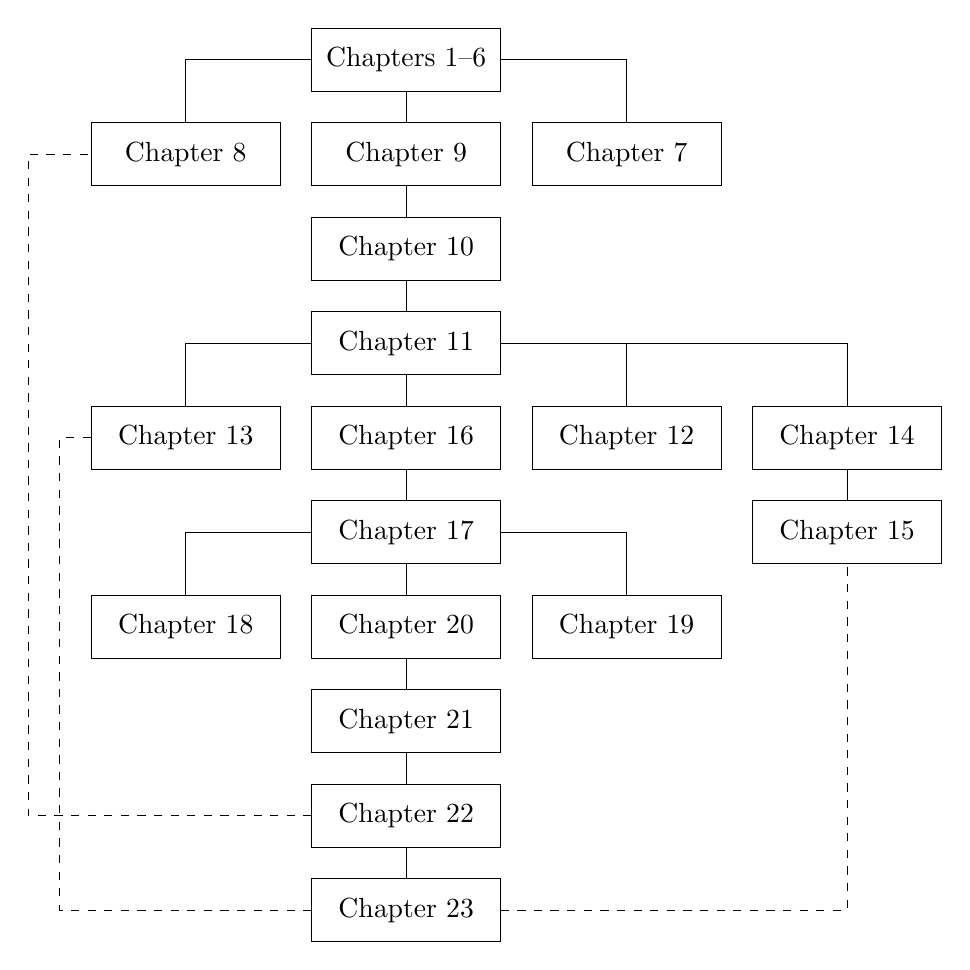
\begin{tikzpicture}[scale=0.8]  %Replaced figure with tikz figure - TWJ 6/14/2010

\draw (3.5,0) rectangle (6.5,1);
\node at (5,0.5) {Chapter 23};

\draw (3.5,1.5) rectangle (6.5,2.5);
\node at (5,2) {Chapter 22};

\draw (3.5,3) rectangle (6.5,4);
\node at (5,3.5) {Chapter 21};

\draw (0,4.5) rectangle (3,5.5);
\node at (1.5,5) {Chapter 18};

\draw (3.5,4.5) rectangle (6.5,5.5);
\node at (5,5) {Chapter 20};

\draw (7,4.5) rectangle (10,5.5);
\node at (8.5,5) {Chapter 19};

\draw (3.5,6) rectangle (6.5,7);
\node at (5,6.5) {Chapter 17};

\draw (10.5,6) rectangle (13.5,7);
\node at (12,6.5) {Chapter 15};

\draw (0,7.5) rectangle (3,8.5);
\node at (1.5,8) {Chapter 13};

\draw (3.5,7.5) rectangle (6.5,8.5);
\node at (5,8) {Chapter 16};

\draw (7,7.5) rectangle (10,8.5);
\node at (8.5,8) {Chapter 12};

\draw (10.5,7.5) rectangle (13.5,8.5);
\node at (12,8) {Chapter 14};

\draw (3.5,9) rectangle (6.5,10);
\node at (5,9.5) {Chapter 11};

\draw (3.5,10.5) rectangle (6.5,11.5);
\node at (5,11) {Chapter 10};

\draw (0,12) rectangle (3,13);
\node at (1.5,12.5) {Chapter 8};

\draw (3.5,12) rectangle (6.5,13);
\node at (5,12.5) {Chapter 9};

\draw (7,12) rectangle (10,13);
\node at (8.5,12.5) {Chapter 7};

\draw (3.5,13.5) rectangle (6.5,14.5);
\node at (5,14) {Chapters 1--6};

\draw (5,1) -- (5,1.5) (5,2.5) -- (5,3)  (5,4) -- (5,4.5)  (5,5.5) -- (5,6)  (5,7) -- (5,7.5)  (5,8.5) -- (5,9)  (5,10) -- (5,10.5)  (5,11.5) -- (5,12)  (5,13) -- (5,13.5);

\draw [dashed] (6.5,0.5) -- (12,0.5) -- (12,6);

\draw (12,7) -- (12,7.5) (12,8.5) -- (12,9.5) -- (6.5,9.5) (8.5,8.5) -- (8.5,9.5);

\draw (8.5,5.5) -- (8.5,6.5) -- (6.5,6.5);

\draw (8.5,13) -- (8.5,14) -- (6.5,14);

\draw [dashed] (3.5,0.5) -- (-0.5,0.5) -- (-0.5,8) -- (0,8);

\draw [dashed] (3.5,2) -- (-1,2) -- (-1,12.5) -- (0,12.5);

\draw (1.5,5.5) -- (1.5,6.5) -- (3.5,6.5);

\draw (1.5,8.5) -- (1.5,9.5) -- (3.5,9.5);

\draw (1.5,13) -- (1.5,14) -- (3.5,14);

\end{tikzpicture}

\end{center}
\end{figure}

Though there are no specific prerequisites for a course in abstract
algebra, students who have had other higher-level courses in
mathematics will generally be more prepared than those who have not,
because they will possess a bit more mathematical sophistication.
Occasionally, we shall assume some basic linear algebra; that is, we
shall take for granted an elementary knowledge of matrices and
determinants. This should present no great problem, since most
students taking a course in abstract algebra have been introduced to
matrices and determinants elsewhere in their career, if they have not
already taken a sophomore- or junior-level course in linear algebra.

Exercise sections are the heart of any mathematics text. An exercise
set appears at the end of each chapter. The nature of the exercises
ranges over several categories; computational,  conceptual, and
theoretical problems are included. A section presenting hints and
solutions to many of the exercises appears at the end of the text.
Often in the solutions a proof is only sketched, and it is up to the
student to provide the details. The exercises range in difficulty from
very easy to very challenging. Many of the more substantial problems
require careful thought, so the student should not be discouraged if
the solution is not forthcoming after a few minutes of work. 
% A complete solutions manual is available for the instructor's use. 
% Removed reference to the solutions manual.  TWJ 8/19/2010

There are additional exercises or computer projects at the ends of
many of the chapters. The computer projects usually require a
knowledge of programming. All of these exercises and projects are more
substantial in nature and allow the exploration of new results and
theory.

% Added Sage blurb, RAB 2011/07/28
Sage (\url{sagemath.org}) is a free, open source, software system
for advanced mathematics, which is ideal for assisting with a study
of abstract algebra. Comprehensive discussion about Sage, and a
selection of relevant exercises, are provided in an electronic
format that may be used with the Sage Notebook in a web browser,
either on your own computer, or at a public server such as
\url{sagenb.org}.  Look for this supplement at the book's
website: \url{abstract.pugetsound.edu}.  In printed
versions of the book, we include a brief description of Sage's
capabilities at the end of each chapter, right after the references.

The open source version of this book has received support from the National Science Foundation (Award \# 1020957).
%Added NSF support statement.  TWJ 8/9/2012

\section*{Acknowledgements}

I would like to acknowledge the following reviewers for their helpful
comments and suggestions. 
\begin{itemize}
 
\item
David Anderson,
University of Tennessee, Knoxville

\item
Robert Beezer,
University of Puget Sound

\item
Myron Hood,
California Polytechnic State University

\item
Herbert Kasube,
Bradley University

\item
John Kurtzke,
University of Portland
 
\item
Inessa Levi,
University of Louisville
 
\item
Geoffrey Mason,
University of California, Santa Cruz

\item
Bruce Mericle,
Mankato State University
 
\item
Kimmo Rosenthal,
Union College

\item
Mark Teply,
University of Wisconsin

\end{itemize}
I would also like to thank Steve Quigley, Marnie Pommett, Cathie
Griffin, Kelle Karshick, and the rest of the staff at PWS for their
guidance throughout this project. It has been a pleasure to work with
them. 

 
\begin{flushright}
Thomas W. Judson
\end{flushright}
 
 
\pagestyle{headings}
 
 
 
 

%
\aatatableofcontents
%
\mainmatter
%
%% TWJ, 2010/03/31
%% Chapters now begin with Chapter 1
%% \setcounter{chapter}{-1}
%
%%%%(c)
%%%%(c)  This file is a portion of the source for the textbook
%%%%(c)
%%%%(c)    Abstract Algebra: Theory and Applications
%%%%(c)    by Thomas W. Judson
%%%%(c)
%%%%(c)    Sage Material
%%%%(c)    Copyright 2011 by Robert A. Beezer
%%%%(c)
%%%%(c)  See the file COPYING.txt for copying conditions
%%%%(c)
%%%%(c)
Sage is free, open source, mathematical software, which has very impressive capabilities for the study of abstract algebra.  See the Preface for more information about obtaining Sage and the supplementary material describing how to use Sage in the study of abstract algebra.  At the end of chapter, we will have a brief explanation of Sage's capabilities relevant to that chapter.     %Set Theory
%%%%(c)
%%%%(c)  This file is a portion of the source for the textbook
%%%%(c)
%%%%(c)    Abstract Algebra: Theory and Applications
%%%%(c)    Copyright 1997 by Thomas W. Judson
%%%%(c)
%%%%(c)  See the file COPYING.txt for copying conditions
%%%%(c)
%%%%(c)
\chap{The Integers}{integers}


 
 
The integers are the building blocks of mathematics. In this chapter we will investigate  the fundamental properties of the integers, including mathematical induction, the division algorithm, and the Fundamental Theorem of Arithmetic.


\section{Mathematical Induction}\label{integers:math_induction}

Suppose we wish to show that
\[
1 + 2 + \cdots + n = \frac{n(n + 1)}{2}
\]
for any natural number $n$. This formula is easily  verified for small numbers such as $n = 1$, 2, 3, or 4, but it is impossible to verify for all natural numbers on a case-by-case basis.  To prove the formula true in general, a more generic method is required.

Suppose we have verified the equation for the first $n$ cases.  We will attempt to show that we can generate the formula for the $(n + 1)$th case from this knowledge.  The formula is true for $n = 1$ since 
\[
1 = \frac{1(1 + 1)}{2}.
\]
If we have verified the first $n$ cases, then
\begin{align*}
1 + 2 + \cdots + n + (n + 1) & = \frac{n(n + 1)}{2} + n + 1 \\
& = \frac{n^2 + 3n + 2}{2} \\
& = \frac{(n + 1)[(n + 1) + 1]}{2}.
\end{align*}
This is exactly the formula for the $(n + 1)$th case.
 
This method of proof is known as \boldemph{mathematical induction}.  Instead of attempting to verify a statement about some subset $S$ of the positive integers ${\mathbb N}$ on a case-by-case basis, an impossible task if $S$ is an infinite set, we give a specific proof for the smallest integer being considered, followed by a generic argument showing that if the statement holds for a given case, then it must also hold for the next  case in the sequence.  We summarize mathematical induction in the following axiom. 

\medskip

\noindent
{\bf First Principle of Mathematical Induction.}\index{Induction!first principle of} 
Let $S(n)$ be a statement about integers for  $n \in {\mathbb N}$ and suppose $S(n_0)$ is true for some integer $n_0$.  If for all integers $k$ with $k \geq n_0$ $S(k)$ implies that $S(k+1)$ is true, then $S(n)$ is true for all integers $n$ greater than or equal to $n_0$.  

%wording change.  Suggested by P. Diethelm.  TWJ 22/4/2013

\begin{example}{induction_greater_than}
For all integers $n \geq 3$, $2^n > n + 4$. Since
\[
8 = 2^3 > 3 + 4 = 7,
\]
the statement is true for $n_0 = 3$.  Assume that $2^k > k + 4$ for $k \geq 3$.  Then $2^{k + 1} = 2 \cdot 2^{k} > 2(k + 4)$.  But 
\[
2(k + 4) = 2k + 8 > k + 5 = (k + 1) + 4
\]
since $k$ is positive.  Hence, by induction, the statement holds for all integers $n \geq 3$. 
\end{example}

\begin{example}{induction_divisible}
Every integer $10^{n + 1} + 3 \cdot 10^n + 5$ is divisible by 9 for $n \in {\mathbb N}$.  For $n = 1$, 
\[
10^{1 + 1} + 3 \cdot 10 + 5 = 135 = 9 \cdot 15
\]
is divisible by 9.  Suppose that $10^{k + 1} + 3 \cdot 10^k + 5$ is divisible by 9 for $k \geq 1$.  Then 
\begin{align*}
10^{(k + 1) + 1} + 3 \cdot 10^{k + 1} + 5
& =
10^{k + 2} + 3 \cdot 10^{k + 1} + 50 - 45 \\
& =
10 (10^{k + 1} + 3 \cdot 10^{k} + 5) - 45
\end{align*}
is divisible by 9.
\end{example}

\begin{example}{binomial_theorem}
We will prove the binomial theorem using mathematical induction; that is, 
\[
(a + b)^n = \sum_{k = 0}^{n} \binom{n}{k} a^k b^{n - k},
\]
where $a$ and $b$ are real numbers, $n \in \mathbb{N}$, and
\[
\binom{n}{k}
= \frac{n!}{k! (n - k)!}\label{factorial}
\]
is the binomial coefficient.\label{binomial}  We first show that
\[
\binom{n + 1}{k}
=
\binom{n}{k} + \binom{n}{k - 1}.
\]
This result follows from
\begin{align*}
\binom{n}{k} + \binom{n}{k - 1}
& =
\frac{n!}{k!(n - k)!}
+\frac{n!}{(k-1)!(n - k + 1)!} \\
& =
\frac{(n + 1)!}{k!(n + 1 - k)!} \\
& =
\binom{n + 1}{k}.
\end{align*}
If $n = 1$, the binomial theorem is easy to verify. Now assume that the result is true for $n$ greater than or equal to 1.  Then
\begin{align*}
(a + b)^{n + 1}
& = 
(a + b)(a + b)^n \\
& =
(a + b) 
\left(
\sum_{k = 0}^{n} \binom{n}{k} a^k b^{n - k}
\right) \\
& = 
\sum_{k = 0}^{n} \binom{n}{k} a^{k + 1} b^{n - k}   +
\sum_{k = 0}^{n} \binom{n}{k} a^k b^{n + 1 - k} \\
& = 
a^{n + 1} + \sum_{k = 1}^{n} \binom{n}{k - 1} a^{k} b^{n + 1 - k} 
 +
\sum_{k = 1}^{n} \binom{n}{k}  a^k b^{n + 1 - k} + b^{n + 1}\\
&  = 
a^{n + 1} + \sum_{k = 1}^{n} \left[ \binom{n}{k - 1}
+
\binom{n}{k} \right]
a^k b^{n + 1 - k} + b^{n + 1} \\
&  = 
\sum_{k = 0}^{n + 1}   \binom{n + 1}{k} a^k b^{n + 1- k}.
\end{align*}
\end{example}
 
We have an equivalent statement of the Principle of Mathematical Induction that is often very useful.
 
\medskip

\noindent 
{\bf Second Principle of Mathematical Induction.}\index{Induction!second principle of}  
Let $S(n)$ be a statement about integers for  $n \in {\mathbb N}$ and suppose $S(n_0)$ is true for some integer $n_0$.  If $S(n_0), S(n_0 + 1), \ldots, S(k)$ imply that $S(k + 1)$ for $k \geq n_0$, then the statement $S(n)$ is true for all integers $n \geq n_0$.   

%wording change.  Suggested by P. Diethelm.  TWJ 22/4/2013
 
\medskip

A  nonempty subset $S$ of ${\mathbb Z}$ is \boldemph{well-ordered\/}\index{Well-ordered set} if $S$ contains a least element.  Notice that the set ${\mathbb Z}$ is not well-ordered since it does not contain a smallest element.  However, the natural numbers are well-ordered. 
 
\medskip
 
\noindent {\bf Principle of Well-Ordering.} 
Every nonempty subset of the natural numbers is well-ordered. 

\medskip
 
The Principle of Well-Ordering is equivalent to the Principle  of Mathematical Induction. 
 
\begin{lemma}\label{integers:smallest_number_lemma}
The Principle of Mathematical Induction implies that $1$ is the least positive natural number. 
\end{lemma}

\begin{proof}
Let $S = \{ n \in {\mathbb N} : n \geq 1 \}$. Then $1 \in S$.  Now assume that $n \in S$; that is, $n \geq 1$.  Since $n+1 \geq 1$, $n+ 1 \in S$; hence, by induction, every natural number is greater than or equal to 1. 
\end{proof}

% Theorem reworded for clarity.  TWJ 12/17/2011
% Suggested by K. Halasz and R. Beezer.
\begin{theorem}\label{integers_PMI_implies_PWO}
The Principle of Mathematical Induction implies the Principle of Well-Ordering.  That is, every nonempty subset of $\mathbb N$ contains a least element.
\end{theorem}
 
\begin{proof}
We must show that if $S$ is a nonempty subset of the natural numbers, then $S$ contains a least element.  If $S$ contains 1, then the theorem is true by Lemma~\ref{integers:smallest_number_lemma}.  Assume that if $S$ contains an integer $k$ such that $1 \leq k \leq n$, then $S$ contains a least element.  We will show that if a set $S$ contains an integer less than or equal to $n + 1$, then $S$ has a least element.  If $S$ does not contain an integer less than $n+1$, then $n+1$ is the smallest integer in $S$.  Otherwise, since $S$ is nonempty, $S$ must contain an integer less than or equal to $n$. In this case, by induction, $S$ contains a least element. 
\hspace*{1in} 
\end{proof}

%wording change.  Suggested by P. Diethelm.  TWJ 22/4/2013
 
\medskip
 
Induction can also be very useful in formulating definitions.  For instance, there are two ways to define $n!$, the factorial of a positive integer $n$. 
\begin{itemize}
 
\item 
The \emph{explicit} definition: $n! = 1 \cdot 2 \cdot 3 \cdots (n - 1)
\cdot n$. 
 
\item 
The \emph{inductive} or \emph{recursive} definition: $1! = 1$ and
$n! = n(n - 1)!$ for $n > 1$. 
 
\end{itemize}
Every good mathematician or computer scientist knows that looking at problems recursively, as opposed to explicitly, often results in better understanding of complex issues.  

 
\section{The Division Algorithm}

An application of the Principle of Well-Ordering that we will use often is the division algorithm. 

\begin{theorem}[Division Algorithm]\label{integers:division_algorithm}\index{Division algorithm!for integers}
Let $a$ and $b$ be integers, with $b > 0$.  Then there exist unique integers $q$ and $r$ such that 
\[
a = bq + r
\]
where $0 \leq r < b$.
\end{theorem}

\begin{proof}
This is a perfect example of the existence-and-uniqueness type of proof.  We must first prove that the numbers $q$ and $r$ actually  exist. Then we must show that if  $q'$ and $r'$ are two other such numbers, then $q = q'$ and $r = r'$. 
 
\emph{Existence of q and r}.
Let
\[
S = \{ a - bk : k \in {\mathbb Z} \text{ and } a - bk \geq 0 \}.
\]
If $0 \in S$, then $b$ divides $a$, and  we can let $q = a/b$ and $r = 0$.  If $0 \notin S$, we can use the Well-Ordering Principle.  We must first show that $S$ is nonempty.  If $a > 0$, then $a - b \cdot 0 \in S$. If $a < 0$, then $a - b(2a) = a(1 - 2b) \in S$.  In either case $S \neq \emptyset$.  By the Well-Ordering Principle, $S$ must have a smallest member, say $r = a - bq$. Therefore, $a = bq + r$, $r \geq 0$. We now show that $r < b$. Suppose that $r > b$. Then   
\[
a - b(q + 1)= a - bq - b = r - b > 0.
\]
In this case we would have $a - b(q + 1)$ in the set $S$. But then $a - b(q + 1) < a - bq$, which would contradict the fact that $r = a - bq$ is the smallest member  of $S$. So $r \leq b$.  Since $0 \notin S$, $r \neq b$ and so $r < b$. 
 
\emph{Uniqueness of q and r}.
Suppose there exist integers $r$, $r'$, $q$, and $q'$ such that
\[
a = bq + r, 0 \leq r < b 
\qquad
\text{and}
\qquad
a = bq' + r', 0 \leq r' < b.
\]
Then $ bq + r =  bq' + r'$.  Assume that $r' \geq r$.  From the last equation we have $b(q - q') = r' - r$; therefore, $b$ must divide $r' - r$ and $0 \leq r'- r \leq r' < b$.  This is possible only if $r' - r = 0$.  Hence, $r = r'$ and  $q = q'$. 
\end{proof}

\medskip

Let $a$ and $b$ be integers.  If $b = ak$ for some integer $k$, we write $a \mid b$\label{divides}.  An integer $d$ is called a \boldemph{common divisor} of $a$ and $b$ if $d \mid a$ and $d \mid b$.  The \boldemph{greatest common divisor}\index{Greatest common divisor!of two integers} of integers $a$ and $b$ is a positive integer $d$ such that $d$ is a common divisor  of $a$ and $b$ and if $d'$ is any other common divisor of $a$ and $b$, then $d' \mid d$.  We write $d = \gcd(a, b)$\label{greatestcd}; for example, $\gcd( 24, 36) = 12$ and $\gcd(120, 102) = 6$.  We say that two integers $a$ and $b$ are \boldemph{relatively prime} if $\gcd( a, b ) = 1$. 

\begin{theorem}\label{integers:gcd_theorem}
Let $a$ and $b$ be nonzero integers. Then there exist integers $r$ and $s$ such that
\[
\gcd( a, b) = ar + bs.
\]
Furthermore, the greatest common divisor of $a$ and $b$ is unique.
\end{theorem}
 
\begin{proof} %Notation error in proof fixed (pointed out by Rocco Rossi) - TWJ 9/13/2010
Let
\[
S = \{ am + bn : m, n \in {\mathbb Z} \text{ and } am + bn > 0 \}.
\]
Clearly, the set $S$ is nonempty; hence, by the Well-Ordering Principle $S$ must have a smallest member, say $d = ar + bs$.  We claim that $d = \gcd( a, b)$.  Write $a = dq + r'$ where $0 \leq r' < d$ . If $r' > 0$, then %r changed to r' - TWJ 1/31/2011
\begin{align*}
r '
& = a - dq \\
& = a - (ar + bs)q \\
& = a - arq - bsq \\
& = a( 1 - rq ) + b( -sq ),
\end{align*}
which is in $S$.  But this would contradict the fact that $d$ is the smallest member of $S$.  Hence, $r' = 0$ and $d$ divides $a$.  A similar argument shows that $d$ divides $b$.  Therefore, $d$ is a common divisor of $a$ and $b$.

Suppose that $d'$ is another common divisor of $a$ and $b$, and we want to show that $d' \mid d$. If we let $a = d'h$ and $b = d'k$, then
\[
d = ar + bs = d'hr + d'ks = d'(hr + ks).
\]
So $d'$ must divide $d$. Hence, $d$ must be the unique greatest common divisor of $a$ and $b$. 
\end{proof}

\begin{corollary}\label{integers:coprime_corollary}
Let $a$ and $b$ be two integers that are relatively prime. Then there exist  integers $r$ and $s$ such that $ar + bs = 1$. 
\end{corollary}
 
 
\subsection*{The Euclidean Algorithm}

Among other things, Theorem~\ref{integers:gcd_theorem} allows us to compute the greatest common divisor of two integers. 

\medskip

\begin{example}{gcd}
Let us compute the greatest common divisor of $945$ and $2415$.  First observe that 
\begin{align*}
2415 & = 945 \cdot 2 + 525 \\
945 & = 525 \cdot 1 + 420 \\
525 & = 420 \cdot 1 + 105 \\
420 & = 105 \cdot 4 + 0.
\end{align*}
Reversing our steps, 105 divides 420, 105 divides 525, 105 divides 945, and 105 divides 2415.  Hence, 105 divides both 945 and 2415.  If $d$ were another common divisor of 945 and 2415, then $d$ would also have to divide 105.  Therefore, $\gcd( 945, 2415 ) = 105$.

If we work backward through the above sequence of equations, we can also obtain numbers $r$ and $s$ such that $945 r + 2415 s = 105$.  Observe that 
\begin{align*}
105 & = 525 + (-1) \cdot 420 \\
& = 525 + (-1) \cdot [945 + (-1) \cdot 525] \\
& = 2 \cdot 525 + (-1) \cdot 945 \\
& = 2 \cdot [2415 + (-2) \cdot 945] + (-1) \cdot 945 \\
& = 2 \cdot 2415 + (-5) \cdot 945.
\end{align*}
So $r = -5$ and $s= 2$.  Notice that $r$ and $s$ are not unique, since $r = 41$ and $s = -16$ would also work.
\end{example}

To compute $\gcd(a,b) = d$, we are using repeated divisions to obtain a decreasing sequence of positive integers $r_1 > r_2 > \cdots > r_n = d$; that is,
\begin{align*}
b & = a q_1 + r_1 \\
a & = r_1 q_2 + r_2 \\
r_1 & = r_2 q_3 + r_3 \\
& \vdots  \\
r_{n - 2} & = r_{n - 1} q_{n} + r_{n} \\
r_{n - 1} & = r_n q_{n + 1}.
\end{align*}
To find $r$ and $s$ such that $ar + bs = d$, we begin with this last equation and substitute results obtained from the previous equations:
\begin{align*}
d & = r_n \\
& = r_{n - 2} - r_{n - 1} q_n \\
& = r_{n - 2} - q_n( r_{n - 3} - q_{n - 1} r_{n - 2} ) \\
& = -q_n r_{n - 3} + ( 1+ q_n q_{n-1} ) r_{n - 2}  \\
& \vdots  \\
& = ra + sb.
\end{align*}
The algorithm that we have just used to find the greatest common divisor $d$ of two integers $a$ and $b$ and to write $d$ as the linear combination of $a$ and $b$ is known as the \boldemph{Euclidean algorithm}\index{Euclidean algorithm}\index{Algorithm!Euclidean}.  
 
 
\subsection*{Prime Numbers}

Let $p$ be an integer such that $p > 1$.  We say that $p$ is a \boldemph{prime number}\index{Prime integer}, or simply $p$ is \boldemph{prime}, if the only positive numbers that divide $p$ are 1 and $p$ itself.  An integer $n > 1$ that is not prime is said to be \boldemph{composite}\index{Composite integer}.  

\begin{lemma}[Euclid]\label{integers:prime_divisor_theorem}
Let $a$ and $b$ be integers and $p$ be a prime number.  If $p \mid ab$, then either $p \mid a$ or $p \mid b$. 
\end{lemma}

\begin{proof}
Suppose that $p$ does not divide $a$.  We must show that $p \mid b$. Since $\gcd( a, p ) = 1$, there exist integers $r$ and $s$ such that $ar + ps = 1$.  So 
\[
b = b(ar + ps) = (ab)r + p(bs).
\]
Since $p$ divides both $ab$ and itself, $p$ must divide $b = (ab)r + p(bs)$. 
\end{proof}

\begin{theorem}[Euclid]\label{integers_inifinite_primes}
There exist an infinite number of primes.
\end{theorem}

\begin{proof}
We will prove this theorem by contradiction.  Suppose that there are only a finite number of primes, say $p_1, p_2, \ldots, p_n$.  Let $P = p_1  p_2  \cdots  p_n + 1$.    Then $P$ must be divisible by some $p_i$ for $1 \leq i \leq n$. In this  case, $p_i$ must divide $P - p_1 p_2 \cdots p_n = 1$, which is a contradiction.  Hence, either $P$ is prime or there exists an additional prime number $p \neq p_i$ that divides $P$.
\end{proof}
%Error in proof fixed.  Suggested by R. Rossi.  TWJ 12/19/2011

\begin{theorem}[Fundamental Theorem of Arithmetic]\label{integers_theorem_FTA}\index{Fundamental Theorem!of Arithmetic}
Let $n$ be an integer such that $n > 1$.  Then
\[
n = p_1 p_2 \cdots p_k,
\]
where $p_1, \ldots, p_k$ are  primes (not necessarily distinct).  Furthermore, this factorization is unique; that is, if 
\[
n = q_1 q_2 \cdots q_l,
\]
then $k = l$ and the $q_i$'s are just the $p_i$'s rearranged.
\end{theorem}

\begin{proof}
\emph{Uniqueness}.
To show uniqueness we will use induction on $n$. The theorem is certainly true for $n = 2$ since in this case $n$ is prime.  Now assume that the result holds for all integers $m$ such that $1 \leq m < n$, and 
\[
n = p_1 p_2 \cdots p_k = q_1 q_2 \cdots q_l,
\]
where $p_1 \leq p_2 \leq \cdots \leq p_k$ and $q_1 \leq q_2 \leq \cdots \leq q_l$. By Lemma~\ref{integers:prime_divisor_theorem}, $p_1  \mid  q_i$ for some $i = 1, \ldots, l$ and $q_1  \mid  p_j$ for some $j = 1, \ldots, k$.  Since all of the $p_i$'s and $q_i$'s are prime, $p_1 = q_i$ and  $q_1 = p_j$. Hence, $p_1 = q_1$ since $p_1 \leq p_j = q_1 \leq q_i = p_1$.  By the induction hypothesis, 
\[
n' = p_2 \cdots p_k = q_2 \cdots q_l
\]
has a unique factorization.  Hence, $k=l$ and $q_i = p_i$ for $i = 1, \ldots, k$. 

\emph{Existence}.
To show existence, suppose that there is some integer that cannot be written as the product of primes.  Let $S$ be the set of all such numbers.  By the Principle of Well-Ordering, $S$ has a smallest number, say $a$.  If the only positive factors of $a$ are $a$ and 1, then $a$ is prime, which is a contradiction.  Hence, $a = a_1 a_2$ where $1 < a_1 < a$ and $1 < a_2 < a$.  Neither $a_1\in S$ nor $a_2 \in S$, since $a$ is the smallest element in $S$.  So 
\begin{align*}
a_1 & = p_1 \cdots p_r \\
a_2 & = q_1 \cdots q_s.
\end{align*}
Therefore,
\[
a = a_1 a_2 = p_1 \cdots p_r q_1 \cdots q_s.
\]
So $a \notin S$, which is a contradiction.
\end{proof}
 
\histhead

\noindent
\parbox{\textwidth}
{\small \histf
Prime numbers were first studied by the ancient Greeks.  Two important results from antiquity are Euclid's proof that an infinite number of primes exist and the Sieve of Eratosthenes, a method of computing all of the prime numbers less than a fixed positive integer $n$.  One problem in number theory is to find a function $f$ such that $f(n)$ is prime for each integer $n$. Pierre Fermat (1601?--1665) conjectured that $2^{2^n} + 1$ was prime for all $n$, but later it was shown by Leonhard Euler (1707--1783) that 
\[
2^{2^5} + 1 = \text{4,294,967,297}
\]
is a composite number. One of the many unproven conjectures about prime numbers is Goldbach's Conjecture.  In a letter to Euler in 1742, Christian Goldbach stated the conjecture that every even integer with the exception of 2 seemed to be the sum of two primes:  $4 = 2 + 2$, $6 = 3 + 3$, $8 =3 + 5$, $\ldots$.  Although the conjecture has been verified for the numbers up through 100 million, it has yet to be proven in general.  Since prime numbers play an important role in public key cryptography, there is currently a great deal of interest in determining whether or not a large number is prime.
\histbox
}


\markright{EXERCISES}
\section*{Exercises}
\exrule

{\small
 
\begin{enumerate}
 
\item
Prove that
\[
1^2 + 2^2 + \cdots + n^2 = \frac{n(n + 1)(2n + 1)}{6}
\]
for $n \in {\mathbb N}$.

\item
Prove that
\[
1^3 + 2^3 + \cdots + n^3 = \frac{n^2(n + 1)^2}{4}
\]
for $n \in {\mathbb N}$.

\item
Prove that $n! > 2^n$ for $n \geq 4$.

\item
Prove that
\[
x + 4x + 7x + \cdots + (3n-2)x = \frac{n(3n - 1)x}{2}
\]
for $n \in {\mathbb N}$.

\item
Prove that $10^{n + 1} + 10^n + 1$ is divisible by 3 for $n \in {\mathbb N}$.

\item
Prove that $4 \cdot 10^{2n} + 9 \cdot 10^{2n - 1} + 5$ is divisible by 99 for $n \in {\mathbb N}$.

\item
Show that
\[
\sqrt[n]{a_1 a_2 \cdots a_n} \leq \frac{1}{n} \sum_{k = 1}^{n} a_k.
\]

\item
Prove the Leibniz rule for $f^{(n)} (x)$, where $f^{(n)}$ is the $n$th derivative of $f$; that is, show that 
\[
(fg)^{(n)} (x) = \sum_{k=0}^{n} \binom{n}{k} f^{(k)}(x) g^{(n-k)} (x).
\]

\item
Use induction to prove that $1 + 2 + 2^2 + \cdots + 2^n = 2^{n + 1} - 1$ for $n \in {\mathbb N}$. 

\item 
Prove that
\[
\frac{1}{2}+ \frac{1}{6} + \cdots + \frac{1}{n(n + 1)} = \frac{n}{n + 1} 
\]
for $n \in {\mathbb N}$.

\item 
If $x$ is a nonnegative real number, then show that $(1 + x)^n - 1 \geq nx$ for $n = 0, 1, 2, \ldots$. 
 
\item
\textbf{Power Sets.} 
Let $X$ be a set.  Define the \boldemph{power set}\index{Power set} of $X$, denoted ${\mathcal P}(X)$\label{powerset}, to be the set of all subsets  of $X$.  For example,  
\[
{\mathcal P}( \{a, b\} ) = \{ \emptyset, \{a\}, \{b\}, \{a, b\} \}.
\]
For every positive integer $n$, show that a set with exactly $n$ elements has a power set with exactly $2^n$ elements.

\item
Prove that the two principles of mathematical induction stated in Section~\ref{integers:math_induction} are equivalent. 

\item
Show that the Principle of Well-Ordering for the natural numbers implies that 1 is the smallest natural number.  Use this result to show that the Principle of Well-Ordering implies the Principle of Mathematical Induction; that is, show that if $S \subset {\mathbb N}$ such that $1 \in S$ and $n + 1 \in S$ whenever $n \in S$, then $S = {\mathbb N}$.  

\item
For each of the following pairs of numbers $a$ and $b$, calculate $\gcd(a,b)$ and find integers $r$ and $s$ such that  $\gcd(a,b) = ra + sb$. 
\begin{multicols}{2}
\begin{enumerate}

\item 
14 and 39

\item
234 and 165

\item
1739 and 9923

\item
471 and 562

\item
23,771 and 19,945

\item
$-4357$ and 3754

\end{enumerate}
\end{multicols}
 
\item 
Let $a$ and $b$ be nonzero integers. If there exist integers $r$ and $s$ such that $ar +bs =1$, show that $a$ and $b$ are relatively prime. 
 
 
\item
\textbf{Fibonacci Numbers.}
The Fibonacci numbers are
\[
1, 1, 2, 3, 5, 8, 13, 21, \ldots.
\]
We can define them inductively by $f_1 = 1$, $f_2 = 1$, and $f_{n + 2} = f_{n + 1} + f_n$ for $n \in {\mathbb N}$. 
\begin{enumerate}
 
 \item
Prove that $f_n < 2^n$.
 
 \item
Prove that $f_{n + 1} f_{n - 1} = f^2_n + (-1)^n$, $n \geq 2$.
 
 \item
Prove that $f_n = [(1 + \sqrt{5}\, )^n - (1 - \sqrt{5}\, )^n]/ 2^n \sqrt{5}$.
 
 \item
Show that $\lim_{n \rightarrow \infty} f_n / f_{n + 1} = (\sqrt{5} - 1)/2$. 
 
 \item
Prove that $f_n$ and $f_{n + 1}$ are relatively prime.
 
\end{enumerate}

\item
Let $a$ and $b$ be integers such that $\gcd(a,b) = 1$.  Let $r$ and $s$ be integers such that $ar + bs =1$.  Prove that 
\[
\gcd(a,s) = \gcd(r,b) = \gcd(r,s) =  1.
\]

\item
Let $x, y \in {\mathbb N}$ be relatively prime.  If $xy$ is a perfect square, prove that $x$ and $y$ must both be perfect squares.

\item
Using the division algorithm, show that every perfect square is of the form $4k$ or $4k + 1$ for some nonnegative integer $k$.

\item
Suppose that $a, b, r, s$ are pairwise relatively prime and that
\begin{align*}
a^2 + b^2 & = r^2 \\
a^2 - b^2 & = s^2.
\end{align*}
Prove that $a$, $r$, and $s$ are odd and $b$ is even.

%% TWJ 9/15/2011
%% Changed "coprime" to "pairwise relatively prime"
%% Suggested by R. Beezer
 
\item
Let $n \in {\mathbb N}$.  Use the division algorithm to prove that every integer is congruent mod $n$ to precisely one of the integers $0, 1, \ldots, n-1$.  Conclude that if $r$ is an integer, then there is exactly one $s$ in ${\mathbb Z}$ such that $0 \leq s < n$ and $[r] = [s]$.   Hence, the integers are indeed partitioned by congruence mod $n$. 

\item
Define the \boldemph{least common multiple} of two nonzero integers $a$ and $b$, denoted by $\lcm(a,b)$\label{leastcm}, to be the nonnegative integer $m$ such that both $a$ and $b$ divide $m$, and if $a$ and $b$  divide any other integer $n$, then $m$ also divides $n$.  Prove that any two integers $a$ and $b$ have a unique least common multiple. 

\item
If $d= \gcd(a, b)$ and $m = \lcm(a, b)$, prove that $dm = |ab|$.

\item
Show that $\lcm(a,b) = ab$ if and only if $\gcd(a,b) = 1$.

\item
Prove that $\gcd(a,c) = \gcd(b,c) =1$ if and only if $\gcd(ab,c) = 1$ for integers $a$, $b$, and $c$.

\item
Let $a, b, c \in {\mathbb Z}$.  Prove that if $\gcd(a,b) = 1$ and $a  \mid bc$, then $a  \mid  c$. 
 
\item
Let $p \geq 2$.  Prove that if $2^p-1$ is prime, then $p$ must also be prime.

\item
Prove that there are an infinite number of primes of the form $6n + 1$. 

\item
Prove that there are an infinite number of primes of the form $4n - 1$.

\item
Using the fact that 2 is prime, show that there do not exist integers $p$ and $q$ such that $p^2 = 2 q^2$.  Demonstrate that therefore $\sqrt{2}$ cannot be a rational number.  

\end{enumerate}
}
 
 
\subsection*{Programming Exercises}
 
{\small
\begin{enumerate}
 
\item
\textbf{The Sieve of Eratosthenes.}\index{Sieve of Eratosthenes}  
One method of computing all of the prime numbers less than a certain fixed positive integer $N$ is to list all of the numbers $n$ such that $1 < n < N$.  Begin by eliminating all of the multiples of 2.  Next eliminate all of the multiples of 3. Now eliminate all of the  multiples of 5.  Notice that 4 has already been crossed out.  Continue in this manner, noticing that we do not have to go all the way to $N$; it suffices to stop at $\sqrt{N}$.  Using this method, compute all of the prime numbers less than $N = 250$.  We can also use this method to find all of the integers that are relatively prime to an integer $N$.  Simply eliminate the prime factors of $N$ and all of their multiples.  Using this method, find all of the numbers that are relatively prime to $N= 120$.  Using the Sieve of Eratosthenes, write a program that will compute all of the primes less than an integer $N$. 

\item
Let ${\mathbb N}^0 = {\mathbb N} \cup \{ 0 \}$. Ackermann's function\index{Ackermann's function} is the function $A :{\mathbb N}^0 \times {\mathbb N}^0 \rightarrow {\mathbb N}^0$ defined by the equations 
\begin{align*}
A(0, y) & = y + 1, \\
A(x + 1, 0) & = A(x, 1), \\
A(x + 1, y + 1) & = A(x, A(x + 1, y)).
\end{align*}
Use this definition to compute $A(3, 1)$.  Write a program to evaluate Ackermann's function.  Modify the  program to count the number of statements executed in the program when Ackermann's function is evaluated.  How many statements are executed in the evaluation of $A(4, 1)$?  What about $A(5, 1)$?

\item
Write a computer program that will implement the Euclidean algorithm.  The program should accept two positive integers $a$ and $b$ as input and should output $\gcd( a,b)$ as well as integers $r$ and $s$ such that 
\[
\gcd( a,b) = ra + sb.
\]
 
\end{enumerate}
}
 
 
\subsection*{References and Suggested Readings} %rReferences updated - TWJ 5/4/2010

{\small
References [2], [3], and [4] are good sources for elementary number
theory. 
\begin{itemize}
 
\item[\textbf{[1]}]
Brookshear, J. G. \textit{Theory of Computation: Formal Languages,
Automata, and Complexity}.  Benjamin/Cummings, Redwood City, CA, 1989.
Shows the relationships of the theoretical aspects of computer science
to set theory and the integers.
 
\item[\textbf{[2]}] %Updated - TWJ 5/4/2010
Hardy, G. H. and Wright, E. M. \textit{An Introduction to the Theory of
Numbers}.  6th ed. Oxford University Press, New York, 2008. 
 
 
\item[\textbf{[3]}] %Checked reference - TWJ 5/4/2010
Niven, I. and Zuckerman, H. S. \textit{An Introduction to the Theory of
Numbers}.  5th ed. Wiley, New York, 1991. 
 
\item[\textbf{[4]}] %Updated - TWJ 5/4/2010
Vanden Eynden, C. \textit{Elementary Number Theory}. 2nd ed.  Waveland Press, Long Grove IL, 2001. 
\end{itemize}
 
}
 
\sagesection %Integers
%%%%(c)
%%%%(c)  This file is a portion of the source for the textbook
%%%%(c)
%%%%(c)    Abstract Algebra: Theory and Applications
%%%%(c)    by Thomas W. Judson
%%%%(c)
%%%%(c)    Sage Material
%%%%(c)    Copyright 2011 by Robert A. Beezer
%%%%(c)
%%%%(c)  See the file COPYING.txt for copying conditions
%%%%(c)
%%%%(c)
These exercises are about becoming comfortable working with groups in Sage.
\begin{sageverbatim}\end{sageverbatim}
%
\sageexercise{1}%
Create the groups \verb?CyclicPermutationGroup(8)? and \verb?DihedralGroup(4)? and give the two groups names of your choosing.  We will understand these constructions better shortly, but for now just understand that they are both groups.
\begin{sageverbatim}\end{sageverbatim}
%
\sageexercise{2}%
Check that the groups have the same size with the \verb?.order()? method.  Determine which is abelian, and which is not, by using the \verb?.is_abelian()? method.
\begin{sageverbatim}\end{sageverbatim}
%
\sageexercise{3}%
Use the \verb?.cayley_table()? method to create the Cayley table for each group.
\begin{sageverbatim}\end{sageverbatim}
%
\sageexercise{4}%
Write a nicely formatted discussion (Shift-click on a blue bar to bring up the mini-word-processor, use dollar signs to embed bits of \TeX) identifying differences between the two groups that are discernible in properties of their Cayley tables.  In other words, what is {\em different} about these two groups that you can ``see'' in the Cayley tables?
\begin{sageverbatim}\end{sageverbatim}
%
\sageexercise{5}%
For each group, use the \verb?.subgroups()? method to locate a largest subgroup that is not the entire group, and then use the \verb?.list()? method of the subgroup to get a list of elements (which you might save as \verb?elts?).\par
%
Now, \verb?.cayley_table(elements=elts)? for the original group will produce the Cayley table of the subgroup.  What properties of this table would you check to see if the output is correct?
\begin{sageverbatim}\end{sageverbatim}
%
\sageexercise{6}%
The \verb?.subgroup(elt_list)? method of the original group will create the smallest subgroup containing specified elements of the group, when given the elements as a list \verb?elt_list?.  Discover the shortest list of elements necessary to recreate the subgroup you used in the previous exercise.  The equality comparison, \verb?==?, can be used to test if two subgroups are equal.
\begin{sageverbatim}\end{sageverbatim}
%
   %Groups
%%%%(c)
%%%%(c)  This file is a portion of the source for the textbook
%%%%(c)
%%%%(c)    Abstract Algebra: Theory and Applications
%%%%(c)    by Thomas W. Judson
%%%%(c)
%%%%(c)    Sage Material
%%%%(c)    Copyright 2011 by Robert A. Beezer
%%%%(c)
%%%%(c)  See the file COPYING.txt for copying conditions
%%%%(c)
%%%%(c)
Cyclic groups are very important, so it is no surprise that they appear in many different forms in Sage.  Each is slightly different, and no one implementation is ideal for an introduction, but together they can illustrate most of the important ideas.  Here is a guide to the various ways to construct, and study, a cyclic group in Sage.
%
\sagesubsection{Infinite Cyclic Groups}
%
In Sage, the integers $\mathbb Z$ are constructed with \verb?ZZ?.  To build the infinite cyclic group such as $3\mathbb Z$ from Example~\ref{example:cyclic:Cyclic_Z3}, simply use \verb?3*ZZ?.  As an infinite set, there is not a whole lot you can do with this.  You can test if integers are in this set, or not.  You can also recall the generator with the \verb?.gen()? command.
%
\begin{sageexample}
sage: G = 3*ZZ
sage: -12 in G
True
sage: 37 in G
False
sage: G.gen()
3
\end{sageexample}
%
\sagesubsection{Additive Cyclic Groups}
%
The additive cyclic group $\mathbb Z_n$ can be built as a special case of a more general Sage construction.  First we build $\mathbb Z_{14}$ and capture its generator.  Throughout, pay close attention to the use of parentheses and square brackets for when you experiment on your own.
%
\begin{sageexample}
sage: G = AdditiveAbelianGroup([14])
sage: G.order()
14
sage: G.list()
[(0), (1), (2), (3), (4), (5), (6), (7),
 (8), (9), (10), (11), (12), (13)]
sage: a = G.gen(0)
sage: a
(1)
\end{sageexample}
%
You can compute in this group, by using the generator, or by using new elements formed by coercing integers into the group, or by taking the result of operations on other elements.  And we can compute the order of elements in this group.  Notice that we can perform repeated additions with the shortcut of taking integer multiples of an element.
%
\begin{sageexample}
sage: a + a
(2)
sage: a + a + a + a
(4)
sage: 4*a
(4)
sage: 37*a
(9)
sage: b = G([2]); b
(2)
sage: b + b
(4)
sage: 2*b == 4*a
True
sage: 7*b
(0)
sage: b.order()
7
sage: c = a - 6*b; c
(3)
sage: c + c + c + c
(12)
sage: c.order()
14
\end{sageexample}
%
It is possible to create cyclic subgroups, from an element designated to be the new generator.  Unfortunately, to do this requires the \verb?.submodule()? method (which should be renamed in Sage).
%
\begin{sageexample}
sage: H = G.submodule([b]); H
Additive abelian group isomorphic to Z/7
sage: H.list()
[(0), (2), (4), (6), (8), (10), (12)]
sage: H.order()
7
sage: e = H.gen(0); e
(2)
sage: 3*e
(6)
sage: e.order()
7
\end{sageexample}
%
The cyclic subgroup \verb?H? just created has more than one generator.  We can test this by building a new subgroup and comparing the two subgroups.
%
\begin{sageexample}
sage: f = 12*a; f
(12)
sage: f.order()
7
sage: K = G.submodule([f]); K
Additive abelian group isomorphic to Z/7
sage: K.order()
7
sage: K.list()
[(0), (2), (4), (6), (8), (10), (12)]
sage: K.gen(0)
(2)
sage: H == K
True
\end{sageexample}
%
Certainly the list of elements, and the common generator of \verb?(2)? lead us to belive that \verb?H? and \verb?K? are the same, but the comparison in the last line leaves no doubt.\par
%
Results in this section, especially Theorem~\ref{cyclic:orders} and Corollary~\ref{cyclic:modngenerators}, can be investigated by creating generators of subgroups from a generator of one additive cyclic group, creating the subgroups, and computing the orders of both elements and orders of groups.
%
\sagesubsection{Abstract Multiplicative Cyclic Groups}
%
We can create an abstract cyclic group in the style of Theorems~\ref{cyclic:cyclicsubgroup}, \ref{cyclic:cyclicabelian}, \ref{cyclic:subgroups}.  In the syntax below \verb?a? is a name for the generator, and \verb?14? is the order of the element.  Notice that the notation is now multiplicative, so we multiply elements, and repeated products can be written as powers.
%
\begin{sageexample}
sage: G.<a> = AbelianGroup([14])
sage: G.order()
14
sage: G.list()
(1, a, a^2, a^3, a^4, a^5, a^6, a^7, a^8, a^9, a^10, a^11, a^12, a^13)
sage: a.order()
14
\end{sageexample}
%
Computations in the group are similar to before, only with different notation.  Now products, with repeated products written as exponentiation.
%
\begin{sageexample}
sage: b = a^2
sage: b.order()
7
sage: b*b*b
a^6
sage: c = a^7
sage: c.order()
2
sage: c^2
1
sage: b*c
a^9
sage: b^37*c^42
a^4
\end{sageexample}
%
Subgroups can be formed with a \verb?.subgroup()? command.  But do not try to list the contents of a subgroup, it'll look strangely unfamiliar.  Also, comparison of subgroups is not implemented.
%
\begin{sageexample}
sage: H = G.subgroup([a^2])
sage: H.order()
7
sage: K = G.subgroup([a^12])
sage: K.order()
7
\end{sageexample}
%
One advantage of this implementation is the possibility to create all possible subgroups.  Here we create the list of subgroups, extract one in particular (the third), and check its order.
%
\begin{sageexample}
sage: allsg = G.subgroups(); allsg
[Multiplicative Abelian subgroup isomorphic to C2 x C7 generated by {a},
 Multiplicative Abelian subgroup isomorphic to C7 generated by {a^2},
 Multiplicative Abelian subgroup isomorphic to C2 generated by {a^7},
 Trivial Abelian subgroup]
sage: sub = allsg[2]
sage: sub.order()
2
\end{sageexample}
%
\sagesubsection{Cyclic Permutation Groups}
%
We will learn more about permutation groups in the next chapter.  But we will mention here that it is easy to create cyclic groups as permutation groups, and a variety of methods are available for working with them, even if the actual elements get a bit cumbersome to work with.  As before, notice that the notation and syntax is multiplicative.
%
\begin{sageexample}
sage: G=CyclicPermutationGroup(14)
sage: a = G.gen(0); a
(1,2,3,4,5,6,7,8,9,10,11,12,13,14)
sage: b = a^2
sage: b = a^2; b
(1,3,5,7,9,11,13)(2,4,6,8,10,12,14)
sage: b.order()
7
sage: a*a*b*b*b
(1,9,3,11,5,13,7)(2,10,4,12,6,14,8)
sage: c = a^37*b^26; c
(1,6,11,2,7,12,3,8,13,4,9,14,5,10)
sage: c.order()
14
\end{sageexample}
%
We can create subgroups, check their orders, and list their elements.
%
\begin{sageexample}
sage: H = G.subgroup([a^2])
sage: H.order()
7
sage: H.gen(0)
(1,3,5,7,9,11,13)(2,4,6,8,10,12,14)
sage: H.list()
[(),
 (1,3,5,7,9,11,13)(2,4,6,8,10,12,14),
 (1,5,9,13,3,7,11)(2,6,10,14,4,8,12),
 (1,7,13,5,11,3,9)(2,8,14,6,12,4,10),
 (1,9,3,11,5,13,7)(2,10,4,12,6,14,8),
 (1,11,7,3,13,9,5)(2,12,8,4,14,10,6),
 (1,13,11,9,7,5,3)(2,14,12,10,8,6,4)]
\end{sageexample}
%
It could help to visualize this group, and the subgroup, as rotations of a regular 12-gon with the vertices labeled with the integers 1 through 12.  This is not the full group of symmetries, since it does not include reflections, just the 12 rotations.
%
\sagesubsection{Cayley Tables}
%
As groups, each of the examples above (groups and subgroups) should have Cayley tables implemented.  Since the groups are cyclic, and their subgroups are therefore cyclic, the Cayley tables should have a similar ``cyclic'' pattern.  Note that the letters used in the default table are generic, and are not related to the letters used above for specific elements --- they just match up with the group elements in the order given by \verb?.list()?.
%
\begin{sageexample}
sage: G.<a> = AbelianGroup([14])
sage: G.cayley_table()
*  a b c d e f g h i j k l m n
 +----------------------------
a| a b c d e f g h i j k l m n
b| b c d e f g h i j k l m n a
c| c d e f g h i j k l m n a b
d| d e f g h i j k l m n a b c
e| e f g h i j k l m n a b c d
f| f g h i j k l m n a b c d e
g| g h i j k l m n a b c d e f
h| h i j k l m n a b c d e f g
i| i j k l m n a b c d e f g h
j| j k l m n a b c d e f g h i
k| k l m n a b c d e f g h i j
l| l m n a b c d e f g h i j k
m| m n a b c d e f g h i j k l
n| n a b c d e f g h i j k l m
\end{sageexample}
%
If the real names of the elements are not too complicated, the table could be more informative using these names.
%
\begin{sageexample}
sage: K.<b> = AbelianGroup([10])
sage: K.cayley_table(names='elements')
  *    1   b b^2 b^3 b^4 b^5 b^6 b^7 b^8 b^9
   +----------------------------------------
  1|   1   b b^2 b^3 b^4 b^5 b^6 b^7 b^8 b^9
  b|   b b^2 b^3 b^4 b^5 b^6 b^7 b^8 b^9   1
b^2| b^2 b^3 b^4 b^5 b^6 b^7 b^8 b^9   1   b
b^3| b^3 b^4 b^5 b^6 b^7 b^8 b^9   1   b b^2
b^4| b^4 b^5 b^6 b^7 b^8 b^9   1   b b^2 b^3
b^5| b^5 b^6 b^7 b^8 b^9   1   b b^2 b^3 b^4
b^6| b^6 b^7 b^8 b^9   1   b b^2 b^3 b^4 b^5
b^7| b^7 b^8 b^9   1   b b^2 b^3 b^4 b^5 b^6
b^8| b^8 b^9   1   b b^2 b^3 b^4 b^5 b^6 b^7
b^9| b^9   1   b b^2 b^3 b^4 b^5 b^6 b^7 b^8
\end{sageexample}
%
\sagesubsection{Complex Roots of Unity}
%
The finite cyclic subgroups of ${\mathbb T}$, generated by a primitive $n$th root of unity are implemented as a more general construction in Sage, known as a cyclotomic field.  If you concentrate on just the multiplication of powers of a generator (and ignore the infinitely many other elements) then this is a finite cyclic group.  Since this is not implemented directly in Sage as a group, {\it per se}, it is a bit harder to construct things like subgroups, but it is an excellent exercise to try.  It is a nice example since the complex numbers are a concrete and familiar construction.  Here are a few sample calculations to provide you with some exploratory tools.  See the notes following the computations.
%
\begin{sageexample}
sage: G = CyclotomicField(14)
sage: w = G.gen(0); w
zeta14
sage: wc = CDF(w)
sage: wc.abs()
1.0
sage: wc.arg()/N(2*pi/14)
1.0
sage: b = w^2
sage: b.multiplicative_order()
7
sage: bc = CDF(b); bc
0.623489801859 + 0.781831482468*I
sage: bc.abs()
1.0
sage: bc.arg()/N(2*pi/14)
2.0
sage: sg = [b^i for i in range(7)]; sg
[1, zeta14^2, zeta14^4,
zeta14^5 - zeta14^4 + zeta14^3 - zeta14^2 + zeta14 - 1,
-zeta14, -zeta14^3, -zeta14^5]
sage: c = sg[3]; d = sg[5]
sage: c*d
zeta14^2
sage: c = sg[3]; d = sg[6]
sage: c*d in sg
True
sage: c*d == sg[2]
True
sage: sg[5]*sg[6] == sg[4]
True
sage: G.multiplication_table(elements=sg)
*  a b c d e f g
 +--------------
a| a b c d e f g
b| b c d e f g a
c| c d e f g a b
d| d e f g a b c
e| e f g a b c d
f| f g a b c d e
g| g a b c d e f
\end{sageexample}
%
Notes:
\begin{enumerate}
%
\item \verb?zeta14? is the name of the generator used for the cyclotomic field, it is a primitive root of unity (a $14$th root of unity in this case).  We have captured it as \verb?w?.
%
\item The syntax \verb?CDF(w)? will convert the complex number \verb?w? into the more familiar form with real and imaginary parts.
%
\item The method \verb?.abs()? will return the modulus of a complex number, $r$ as described in the text.  For elements of ${\mathbb C}^\ast$ this should always equal $1$.
%
\item The method \verb?.arg()? will return the argument of a complex number, $\theta$ as described in the text.  Every element of the cyclic group in this example should have an argument that is an integer multiple of $\frac{2\pi}{14}$.  The \verb?N()? syntax converts the symbolic value of \verb?pi? to a numerical approximation.
%
\item \verb?sg? is a list of elements that form a cyclic subgroup of order 7, composed of the first 7 powers of \verb?b = w^2?.  So, for example, the last comparison multiplies the fifth power of \verb?b? with the sixth power of \verb?b?, which would be the eleventh power of \verb?b?.  But since \verb?b? has order 7, this reduces to the fourth power.
%
If you know a subset of an infinite group forms a subgroup, then you can produce its Cayley table by specifying the list of elements you want to use.  Here we ask for a multiplication table, since that is the relevant operation.
%
\end{enumerate}
%
   %Cyclic Groups
%%%%(c)
%%%%(c)  This file is a portion of the source for the textbook
%%%%(c)
%%%%(c)    Abstract Algebra: Theory and Applications
%%%%(c)    by Thomas W. Judson
%%%%(c)
%%%%(c)    Sage Material
%%%%(c)    Copyright 2011 by Robert A. Beezer
%%%%(c)
%%%%(c)  See the file COPYING.txt for copying conditions
%%%%(c)
%%%%(c)
These exercises are designed to help you become familiar with permutation groups in Sage.
%
\begin{sageverbatim}\end{sageverbatim}
%
\sageexercise{1}%
Create the full symmetric group $S_{10}$ with the command \verb?G = SymmetricGroup(10)?.
\begin{sageverbatim}\end{sageverbatim}
%
\sageexercise{2}
Create elements of \verb?G? with the following (varying) syntax.  Pay attention to commas, quotes, brackets, parentheses.  The first two use a string (characters) as input, mimicking the way we write permuations (but with commas).  The second two use a list of tuples.\par\noindent
\verb?a = G("(5,7,2,9,3,1,8)")?\\
\verb?b = G("(1,3)(4,5)")?\\
\verb?c = G([(1,2),(3,4)])?\\
\verb?d = G([(1,3),(2,5,8),(4,6,7,9,10)])?\par\noindent
%
(a)  Compute $a^3$, $bc$, $ad^{-1}b$.\par\noindent
%
(b)  Compute the orders of each of these four individual elements (\verb?a? through \verb?d?) using a single permutation group element method.\par\noindent
%
(c)  Use the permutation group element method \verb?.sign()? to determine if $a,b,c,d$ are even or odd permutations.\par\noindent
%
(d)  Create two cyclic subgroups of $G$ with the commands:
%
\begin{itemize}
\item\verb?H = G.subgroup([a])?
\item\verb?K = G.subgroup([d])?
\end{itemize}
%
List, and study, the elements of each subgroup.  Without using Sage, list the order of each subgroup of $K$.  Then use Sage to construct a subgroup of $K$ with order 10.\par\noindent
%
(e)  More complicated subgroups can be formed by using two or more generators.  Construct a subgroup $L$ of $G$ with the command \verb?L = G.subgroup([b,c])?.  Compute the order of $L$ and list all of the elements of $L$.
\begin{sageverbatim}\end{sageverbatim}
%
\sageexercise{3}
Construct the group of symmetries of the tetrahedron (also the alternating group on 4 symbols, $A_4$) with the command \verb?A=AlternatingGroup(4)?.  Using tools such as orders of elements, and generators of subgroups, see if you can find \emph{all of} the subgroups of $A_4$ (each one exactly once).  Do this without using the \verb?.subgroups()? method to justify the correctness of your answer (though it might be a convenient way to check your work).\par
%
Provide a nice summary as your answer - not just piles of output.  So use Sage as a tool, as needed, but basically your answer will be a concise paragraph and/or table.  This is the one part of this assignment without clear, precise directions, so spend some time on this portion to get it right.  Hint: no subgroup of $A_4$ requires more than two generators.
\begin{sageverbatim}\end{sageverbatim}
%
\sageexercise{4}
Save your work, and then see if you can crash your Sage session with the commands.  Do not submit the list of elements of \verb?N? as part of your submitted worksheet.
%
\begin{itemize}
\item\verb?N = G.subgroup([b,d])?
\item\verb?N.list()?
\end{itemize}
%
How big is $N$?
\begin{sageverbatim}\end{sageverbatim}
%
\sageexercise{5}
Answer the five questions above about the permutations of the cube expressed as permutations of the 8 vertices.
\begin{sageverbatim}\end{sageverbatim}
%
  %Permutation Groups
%%%%(c)
%%%%(c)  This file is a portion of the source for the textbook
%%%%(c)
%%%%(c)    Abstract Algebra: Theory and Applications
%%%%(c)    by Thomas W. Judson
%%%%(c)
%%%%(c)    Sage Material
%%%%(c)    Copyright 2011 by Robert A. Beezer
%%%%(c)
%%%%(c)  See the file COPYING.txt for copying conditions
%%%%(c)
%%%%(c)
Sage can create all of the cosets of a subgroup, and all of the subgroups of a group.  While these methods can be somewhat slow, they are in many, many ways much better than experimenting with pencil and paper, and can greatly assist us in understanding the structure of finite groups.\par
%
\sagesubsection{Cosets}
%
Sage will create all the right (or left) cosets of a subgroup.  Written mathematically, cosets are sets, and the order of the elements within the set is irrelevant.  With Sage, lists are more natural, and here it is to our advantage.\par
%
Sage creates the cosets of a subgroup as a list of lists.  Each inner list is a single coset.  The first coset is always the coset that is the subgroup itself, and the first element of this coset is the identity.  Each of the other cosets can be construed to have their first element as their representative, and if you use this element as the representative, the elements of the coset are in the same order they would be created by multiplying this representative by the elements of the first coset (the subgroup).\par
%
The keyword \verb?side? can be \verb?'right'? or \verb?'left'?, and if not given, then the default is right cosets.  The options refer to which side of the product has the representative.  Notice that now Sage's results will be ``backwards'' compared with the text.  Here is Example~\ref{example:cosets:S3_Cosets} reprised, but in a slightly different order.
%
\begin{sageexample}
sage: G = SymmetricGroup(3)
sage: a = G("(1,2)")
sage: H = G.subgroup([a])
sage: rc = G.cosets(H, side='right'); rc
[[(), (1,2)], [(2,3), (1,3,2)], [(1,2,3), (1,3)]]
sage: lc = G.cosets(H, side='left'); lc
[[(), (1,2)], [(2,3), (1,2,3)], [(1,3,2), (1,3)]]
\end{sageexample}
%
So if we work our way through the brackets carefully we can see the difference between the right cosets and the left cosets.  Compare these cosets with the ones in the text and see that left and right are reversed.  Shouldn't be a problem --- just keep it in mind.
%
\begin{sageexample}
sage: G = SymmetricGroup(3)
sage: b = G("(1,2,3)")
sage: H = G.subgroup([b])
sage: rc = G.cosets(H, side='right'); rc
[[(), (1,2,3), (1,3,2)], [(2,3), (1,3), (1,2)]]
sage: lc = G.cosets(H, side='left'); lc
[[(), (1,2,3), (1,3,2)], [(2,3), (1,2), (1,3)]]
\end{sageexample}
%
If we study the backeting, we can see that the left and right cosets are equal.  Let's see what Sage thinks:
%
\begin{sageexample}
sage: rc == lc
False
\end{sageexample}
%
Mathematically, we need sets, but Sage is working with ordered lists, and the order matters.  However, if we know our lists do not have duplicates (the \verb?.cosets()? method will never produce duplicates) then we can sort the lists and a test for equality will perform as expected.  The elements of a permutation group have an ordering defined for them --- it is not so important \emph{what} this is, just that \emph{some} ordering is defined.  The \verb?sorted()? function will take any list and return a sorted version.  So for each list of cosets, we will sort the individual cosets and then sort the list of sorted cosets.  This is a typical maneuver, though a bit complicated with the nested lists.
%
\begin{sageexample}
sage: rc_sorted = sorted([sorted(coset) for coset in rc])
sage: rc_sorted
[[(), (1,2,3), (1,3,2)], [(2,3), (1,2), (1,3)]]
sage: lc_sorted = sorted([sorted(coset) for coset in lc])
sage: lc_sorted
[[(), (1,2,3), (1,3,2)], [(2,3), (1,2), (1,3)]]
sage: rc_sorted == lc_sorted
True
\end{sageexample}
%
The list of all cosets can be quite long (it will include every element of the group) and can take a few seconds to complete, even for small groups.  There are more sophisticated, and faster, ways to study cosets (such as just using their representatives), but to understand these techniques you also need to understand more theory.
%
\sagesubsection{Subgroups}
%
Sage can compute all of the subgroups of a group.  This can produce even more output than the coset method and can sometimes take much longer, depending on the structure of the group.  The list is in order of the size of the subgroups, with smallest first.  As a demonstration we will first compute and list all of the subgroups of a small group, and then extract just one of these subgroups from the list for some futher study.
%
\begin{sageexample}
sage: G = SymmetricGroup(3)
sage: sg = G.subgroups(); sg
[Permutation Group with generators [()],
 Permutation Group with generators [(2,3)],
 Permutation Group with generators [(1,2)],
 Permutation Group with generators [(1,3)],
 Permutation Group with generators [(1,2,3)],
 Permutation Group with generators [(2,3), (1,2,3)]]
sage: H = sg[4]; H
Permutation Group with generators [(1,2,3)]
sage: H.order()
3
sage: H.list()
[(), (1,2,3), (1,3,2)]
sage: H.is_cyclic()
True
\end{sageexample}
%
The output of the \verb?.subgroups()? method can be voluminous, so sometimes we are interested in properties of specific subgroups (as in the previous example) or broader questions of the group's ``subgroup structure.''  Here we expand on Corollary~\ref{cosets_theorem_10}.  Notice that just because Sage does not \emph{compute} a subgroup of order 6 in $A_4$, this is no substitute whatsoever for a \emph{proof} such as given for the corollary.  But the computational result emboldens us to search for the theoretical result with confidence.
%
\begin{sageexample}
sage: G = AlternatingGroup(4)
sage: sg = G.subgroups()
sage: [H.order() for H in sg]
[1, 2, 2, 2, 3, 3, 3, 3, 4, 12]
\end{sageexample}
%
So we see no subgroup of oder 6 in the list of subgroups of $A_4$.  Notice how Lagrange's Theorem (Theorem~\ref{LagrangeTheorem} is in evidence --- all the subgroup orders divide $12$, the order of $A_4$.  Be patient, the next subgroup computation may take a while.
%
\begin{sageexample}
sage: G = SymmetricGroup(4)
sage: sg = G.subgroups()
sage: [H.order() for H in sg]
[1, 2, 2, 2, 2, 2, 2, 2, 2, 2, 3, 3, 3, 3, 4, 4, 4, 4, 4, 4, 4,
 6, 6, 6, 6, 8, 8, 8, 12, 24]
\end{sageexample}
%
Again, note Lagrange's Theorem in action.  But more interestingly, $S_4$ has a subgroup of order 6.  Four of them, to be precise.  these four subgroups of order 6 are similar to each other, can you describe them simply (\emph{before} digging into the \verb?sg? list for more information)?  If you were curious how many subgroups $S_4$ has, you could simply count the number of subgroups in the \verb?sg? list.  The \verb?len()? function does this for \emph{any} list and is often an easy way to count things.
%
\begin{sageexample}
sage: len(sg)
30
\end{sageexample}
%
\sagesubsection{Subgroups of Cyclic Groups}
%
Now that we are more familiar with permutation groups, and know about the \verb?.subgroups()? method, we can revisit an idea from Chapter~\ref{cyclic}.  The subgroups of a cyclic group are always cyclic, but how many are there and what are their orders?
%
\begin{sageexample}
sage: G = CyclicPermutationGroup(20)
sage: [H.order() for H in G.subgroups()]
[1, 2, 4, 5, 10, 20]
\end{sageexample}
%
\begin{sageexample}
sage: G = CyclicPermutationGroup(19)
sage: [H.order() for H in G.subgroups()]
[1, 19]
\end{sageexample}
%
We could do this all day, but you have Sage at your disposal, so vary the order of \verb?G? by changing \verb?n? and study the output across many runs.  Maybe try a cyclic group of order 24 and compare with the symmetric group $S_4$ (above) which also has order 24.  Do you feel a conjecture coming on?
%
\begin{sageexample}
sage: n = 8
sage: G = CyclicPermutationGroup(n)
sage: [H.order() for H in G.subgroups()]
[1, 2, 4, 8]
\end{sageexample}
%
\sagesubsection{Euler Phi Function}
%
To add to our number-theoretic functions from Chapter~\ref{integers}, we note that Sage makes the Euler $\phi$-function available as the function \verb?euler_phi()?.
%
\begin{sageexample}
sage: euler_phi(345)
176
\end{sageexample}
%
Here's an interesting experiment that you can try running several times.
%
\begin{sageverbatim}
sage: m = random_prime(10000)
sage: n = random_prime(10000)
sage: m, n, euler_phi(m*n) == euler_phi(m)*euler_phi(n)  # random
(5881, 1277, True)
\end{sageverbatim}
%
Feel another conjecture coming on?  Can you generalize this result?
%
\begin{sageverbatim}
\end{sageverbatim}
%
   %Cosets and Lagrange's Theorem
%%%%(c)
%%%%(c)  This file is a portion of the source for the textbook
%%%%(c)
%%%%(c)    Abstract Algebra: Theory and Applications
%%%%(c)    by Thomas W. Judson
%%%%(c)
%%%%(c)    Sage Material
%%%%(c)    Copyright 2011 by Robert A. Beezer
%%%%(c)
%%%%(c)  See the file COPYING.txt for copying conditions
%%%%(c)
%%%%(c)
With Sage's excellent implementations of basic number-theory computations, it is easy to work non-trivial examples of RSA and the exercises about primality and factoring.    %Cryptography
%%%%(c)
%%%%(c)  This file is a portion of the source for the textbook
%%%%(c)
%%%%(c)    Abstract Algebra: Theory and Applications
%%%%(c)    Copyright 1997 by Thomas W. Judson
%%%%(c)
%%%%(c)  See the file COPYING.txt for copying conditions
%%%%(c)
%%%%(c)
\chap{Algebraic Coding Theory}{algcodes}
 

Coding theory is an application of algebra that has become
increasingly important over the last several decades. When we transmit
data, we are concerned about sending a message over a channel that
could be affected by ``noise.'' We wish to be able to encode and
decode the information in a manner that will allow the detection, and
possibly the correction, of errors caused by noise. This situation
arises in many areas of communications, including radio, telephone,
television, computer communications, and even compact disc player
technology. Probability, combinatorics, group theory, linear algebra,
and polynomial rings over finite fields all play important roles in
coding theory.  
 

\section{Error-Detecting and Correcting Codes}

Let us examine a simple model of a communications system for
transmitting and receiving coded messages (Figure~\ref{encoding}).  

\begin{figure}[htb] %Replaced figure with tikz figure - TWJ 5/10/2010
\begin{center}
\tikzpreface{algcode_encode_decode}
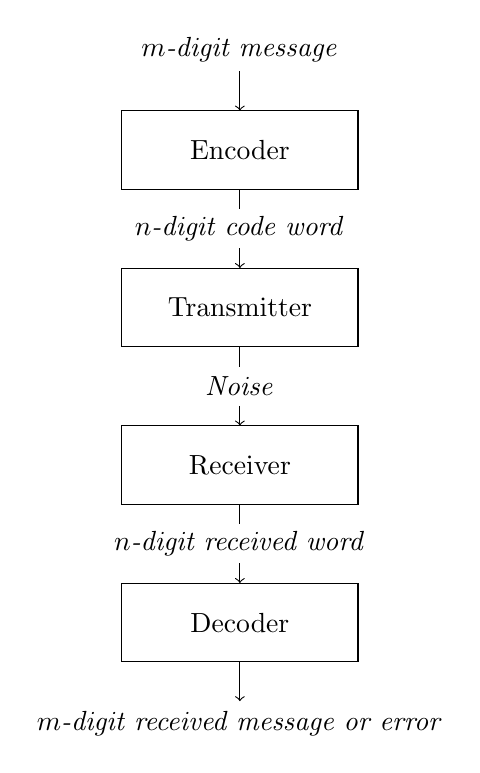
\begin{tikzpicture}[scale=1]

\draw [->] (0,8)  node [above] {\emph{$m$-digit message}} -- (0,7.5);

\node at (0,7) {Encoder};
\draw (-1.5,6.5) rectangle (1.5,7.5);
\draw (0,6.5)  -- (0,6.25);
\draw [->] (0,5.75)  -- (0,5.5);
\node at (0,6) {\emph{$n$-digit code word}};

\node at (0,5) {Transmitter};
\draw (-1.5,4.5) rectangle (1.5,5.5);
\draw (0,4.5)  -- (0,4.25);
\draw [->] (0,3.75)  -- (0,3.5);
\node at (0,4) {\emph{Noise}};

\node at (0,3) {Receiver};
\draw (-1.5,2.5) rectangle (1.5,3.5);
\draw (0,2.5)  -- (0,2.25);
\draw [->] (0,1.75)  -- (0,1.5);
\node at (0,2) {\emph{$n$-digit received word}};

\node at (0,1) {Decoder};
\draw (-1.5,0.5) rectangle (1.5,1.5);
\draw [->] (0,0.5)  -- (0,0) node [below] {\emph{$m$-digit received message or error}};

\end{tikzpicture}

\caption{Encoding and decoding messages}
\end{center}
\label{encoding}
\end{figure}

Uncoded messages may be composed of letters or characters, but
typically they consist of binary $m$-tuples. These messages are
encoded into codewords, consisting of binary $n$-tuples, by a device
called an \boldemph{encoder}. The message is transmitted and then decoded.
We will consider the occurrence of errors during transmission. An
\boldemph{error} occurs if there is a change in one or more bits in the
codeword. A \boldemph{decoding scheme} is a method that either converts
an arbitrarily received $n$-tuple into a meaningful decoded message or
gives an error message for that $n$-tuple. If the received message is
a codeword (one of the special $n$-tuples allowed to be transmitted),
then the decoded message must be the unique message that was encoded
into the codeword. For received non-codewords, the decoding scheme will
give an error indication, or, if we are more clever, will actually try
to correct the error and reconstruct the original message. Our goal is
to transmit error-free messages as cheaply and quickly as possible.
 
 
\begin{example}{repeat}
One possible coding scheme would be to send a message several
times and to compare the received copies with one another. Suppose
that the message to be encoded is a binary $n$-tuple $(x_{1}, x_{2},
\ldots, x_{n})$. The message is encoded into a binary $3n$-tuple by
simply repeating the message three times: 
\[
(x_{1}, x_{2}, \ldots, x_{n})
\mapsto
(x_{1}, x_{2}, \ldots, x_{n}, x_{1}, x_{2}, \ldots, x_{n},
x_{1}, x_{2}, \ldots, x_{n}).
\]
To decode the message, we choose as the $i$th digit the one that
appears in the $i$th place in at least two of the three transmissions.
For example, if the original message is $(0110)$, then the transmitted
message will be \mbox{$(0110\;  0110\;  0110)$}. If there is a transmission error
in the fifth digit, then the received codeword will be
$(0110\;  1110\;  0110)$, which will be correctly decoded as
$(0110)$.\footnote{We will adopt the convention that bits are numbered
left to right in binary $n$-tuples.} 
This triple-repetition method will automatically detect and correct
all single errors, but it is slow and inefficient: to send a message
consisting of $n$ bits, $2n$ extra bits are required, and we can only
detect and correct single errors. We will see that it is possible to
find an encoding scheme that will encode a message of $n$ bits into
$m$ bits with $m$ much smaller than $3n$.
\end{example}
 
 
\begin{example}{even_parity}
\boldemph{Even parity}, a  commonly  used coding scheme, is much
more efficient than the simple repetition scheme. The ASCII (American
Standard Code for Information Interchange) coding system uses binary
8-tuples, yielding $2^{8} = 256$ possible 8-tuples. However, only seven
bits are needed since there are only $2^7 = 128$ ASCII characters.
What can or should be done with the extra bit? Using the full eight
bits, we can detect single transmission errors. For example, the ASCII
codes for A, B, and C are 
\begin{align*}
\mbox{A} & = 65_{10} = 01000001_{2}, \\
\mbox{B} & = 66_{10} = 01000010_{2}, \\
\mbox{C} & = 67_{10} = 01000011_{2}.
\end{align*}
Notice that the leftmost bit is always set to 0; that is, the 128 ASCII
characters have codes 
\begin{align*}
00000000_{2} & = 0_{10}, \\
& \vdots \\
01111111_{2} & = 127_{10}.
\end{align*}
The bit can be used for error checking on the other seven bits. It is
set to either 0 or 1 so that the total number of 1 bits in the
representation of a character is even. Using even parity, the codes
for A, B, and C now become 
\begin{align*}
\mbox{A} & = 01000001_{2}, \\
\mbox{B} & = 01000010_{2}, \\
\mbox{C} & = 11000011_{2}.
\end{align*}
Suppose an A is sent and a transmission error in the sixth
bit is caused by noise over the communication channel so that 
(0100\; 0101) is received. We know an error has occurred since the
received word has an odd number of 1's, and we can now request that the
codeword be transmitted again. When used for error checking, the
leftmost bit is called a \boldemph{parity check bit}.  
 
 
By far the most common error-detecting
codes used in computers are based on the addition of a parity bit.
Typically, a computer stores information in $m$-tuples called \boldemph{
words}. Common word lengths are 8, 16, and 32 bits. One bit in the 
word is set aside as the parity check bit, and is not used to store
information. This bit is set to either 0 or 1, depending on the
number of 1's in the word. 
 
 
Adding a parity check bit allows the detection of all single errors
because changing a single bit either increases or decreases the number
of 1's by one, and in either case the parity has been changed from
even to odd, so the new word is not a codeword. (We could also
construct an error detection scheme based on \boldemph{odd parity}; that
is, we could set the parity check bit so that a codeword always has an
odd number of 1's.)  
\end{example}
 
 
The even parity system is easy to implement, but has two drawbacks.
First, multiple errors are not detectable. Suppose an A is sent and 
the first and seventh bits are changed from 0 to 1. The received word
is a codeword, but will be decoded into a C instead of an A.
Second, we do not have the ability to correct errors.  If the 8-tuple
(1001\; 1000) is received, we know that an error has occurred, but we
have no idea which bit has been changed. We will now investigate a
coding scheme that will not only allow us to detect transmission
errors but will actually correct the errors. 

 
 
\begin{table}[htb]\label{repetition_code}
\begin{center}{\small
\begin{tabular}{|lc|cccccccc|}
\hline
& & \multicolumn{8}{|c|}{Received Word}    \\
            &     & 000 & 001 & 010 & 011 & 100 & 101 & 110
& 111 \\ \hline
Transmitted & 000 & 0   & 1   & 1   & 2   & 1   & 2   & 2
& 3 \\
Codeword   & 111 & 3   &  2  & 2   &  1  &  2  &   1 &  1
&  0 \\ \hline
\end{tabular}
}
\caption{A repetition code}
\end{center}
\end{table}

 
\begin{example}{nearest}
Suppose that our original message is either a 0 or a 1, and that 0
encodes to (000) and 1 encodes to (111). If only a single
error occurs during transmission, we can detect and correct the
error. For example, if a 101 is received, then the second bit must
have been changed from a 1 to a 0.  The originally transmitted
codeword must have been (111). 	This method will detect and correct 
all single errors. 
 
 
In Table~\ref{repetition_code}, we present all possible words that might be received
for the transmitted codewords (000) and (111). Table~\ref{repetition_code} also shows 
the number of bits by which each received 3-tuple differs from each
original codeword. 
\end{example}
 
 
 
\subsection*{Maximum-Likelihood Decoding}

%% Footnote in subsection header undigestable by tex4ht
%%   it can follow just outside the {},
%%   but formats weirdly in both PDF and XHTML
%% \footnote{This section
%% requires a knowledge of probability, but can be
%% skipped without loss of continuity.}

%Label repaired.  Suggested by R. Beezer.
%TWJ - 12/19/2011
The coding scheme presented in Example~\ref{example:algcodes:nearest} is not a complete solution to
the problem because it does not account for the possibility of
multiple errors. For example, either a (000) or a (111) could be sent
and a (001) received. We have no means of deciding from the received
word whether there was a single error in the third bit or two errors,
one in the first bit and one in the second.  No matter what coding 
scheme is used, an incorrect message could
be received: we could transmit a (000), have errors in all three
bits, and receive the codeword (111). It is important to make explicit
assumptions about the likelihood and distribution of transmission
errors so that, in a particular application, it will be known whether
a given
error detection scheme is appropriate. We will assume that
transmission errors are rare, and, that when they do occur, they occur
independently in each bit; that is, if $p$ is the probability of an
error in one bit and $q$ is the probability of an error in a different
bit, then the probability of errors occurring in both of these bits at
the same time is $pq$. We will also assume that a received $n$-tuple 
is
decoded into a codeword that is closest to it; that is, we assume that
the receiver uses \boldemph{maximum-likelihood
decoding}\index{Maximum-likelihood decoding}.
 
 
\begin{figure}[htb]  %Replaced figure with tikz figure - TWJ 5/10/2010
\begin{center}
\tikzpreface{algcode_binary_channel}
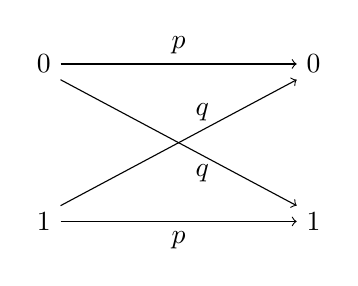
\begin{tikzpicture}[scale=1]

\node at (1.5,0) [below] {$p$};
\draw [->] (0,0)  node [left] {1} -- (3,0) node [right] {1};
\node at (1.5,2) [above] {$p$};
\draw [->] (0,2)  node [left] {0} -- (3,2) node [right] {0};

\draw [->] (0,0.2) -- (3,1.8);
\draw [->] (0,1.8) -- (3,0.2);

\node at (1.8,1.15) [above] {$q$};
\node at (1.8,0.85) [below] {$q$};


\end{tikzpicture}

\end{center}
\caption{Binary symmetric channel}
\label{channel}
\end{figure}
 
 
 
A \boldemph{binary symmetric channel}\index{Binary symmetric channel}
is a model that consists of a transmitter capable of sending a binary 
signal, either a 0 or a 1, together with a receiver. Let $p$ be the 
probability that the signal is correctly
received. Then $q=1-p$ is the probability of an incorrect reception.
If a 1 is sent, then the probability that a 1 is received is $p$ and
the probability that a 0 is received is $q$ (Figure~\ref{channel}).
The probability that no errors occur during the transmission of a binary
codeword of length $n$ is $p^{n}$. For example, if $p=0.999$ and a
message consisting of 10,000 bits is sent, then the probability of a
perfect transmission is 
\[
(0.999)^{10,000} \approx 0.00005.
\]
 
 
\begin{theorem}
If a binary $n$-tuple $(x_{1}, \ldots, x_{n})$ is transmitted across a
binary symmetric channel with probability $p$ that no error will occur
in each coordinate, then the probability that there are errors in
exactly $k$ coordinates~is
\[
\binom{n}{k} q^kp^{n-k}.
\]
\end{theorem}
 
 
\begin{proof}
Fix $k$ different coordinates. We first compute the probability that
an error has occurred in this fixed set of coordinates. The
probability of an error occurring in a particular one of these $k$
coordinates is $q$; the probability that an error will not occur
in any of the remaining $n-k$ coordinates is $p$. The
probability of each of these $n$ independent events is
$q^{k}p^{n-k}$. The number of possible error patterns with exactly $k$
errors occurring is equal to 
\[
\binom{n}{k} 
= \frac{n!}{k!(n-k)!},
\]
the number of combinations of $n$ things taken $k$ at a time. Each of
these error patterns has probability $q^{k}p^{n-k}$ of occurring;
hence, the probability of all of these error patterns is
\[
\binom{n}{k} 
q^{k}p^{n-k}.
\]
\end{proof}
 
 
\begin{example}{probability}
Suppose that $p = 0.995$ and a 500-bit message is sent. The
probability that the message was sent error-free is 
\[
p^{n} = (0.995)^{500} \approx 0.082.
\]
The probability of exactly one error occurring is
\[
\binom{n}{1} 
qp^{n-1}= 500(0.005)(0.995)^{499}
\approx 0.204.
\]
The probability of exactly two errors is
\[
\binom{n}{2} 
q^{2}p^{n-2}=
\frac{500 \cdot 499}{2}(0.005)^{2}(0.995)^{498} \approx
0.257.
\]
The probability of more than two errors is approximately
\[
1-0.082-0.204 -0.257=0.457.
\]
\end{example}
 
 
\subsection*{Block Codes}
 
 
If we are to develop efficient error-detecting and error-correcting
codes, we will need more sophisticated mathematical tools.  Group
theory  will allow faster methods of encoding and decoding messages. A
code is an $(n, m)$-\boldemph{block code} if the information that is to be
coded can be divided into blocks of $m$ binary digits, each of which
can be encoded into $n$ binary digits. More specifically, an $(n,
m)$-block code consists of an \boldemph{encoding function} 
\[
E:{\mathbb Z}^{m}_{2} \rightarrow {\mathbb Z}^{n}_{2}
\]
and a \boldemph{decoding function}
\[
D:{\mathbb Z}^{n}_{2} \rightarrow {\mathbb Z}^{m}_{2}.
\]
A \boldemph{codeword} is any element in the image of $E$. We also require
that $E$ be one-to-one so that two information blocks will not be
encoded into the same codeword. If our code is to be error-correcting,
then $D$ must be onto.
 
 
\begin{example}{BlockCode}
The even-parity coding system developed to detect single errors in
ASCII characters is an $(8,7)$-block code. The encoding function is
\[
E(x_7, x_6, \ldots, x_1) = (x_8, x_7,  \ldots, x_1),
\]
where $x_8 = x_7 + x_6 + \cdots + x_1$ with addition in ${\mathbb Z}_2$. 
\end{example}
 

 
Let ${\mathbf x} = (x_1, \ldots, x_n)$ and ${\mathbf y} = (y_1, \ldots,
y_n)$ be binary $n$-tuples. The \boldemph{Hamming distance}\index{Hamming
distance} or \boldemph{distance}, $d({\mathbf x}, {\mathbf
y})$\label{noteHammingdist}, between ${\mathbf x}$ and ${\mathbf y}$ is
the number of bits in which ${\mathbf x}$ and ${\mathbf y}$ differ. The
distance between two codewords is the minimum number of transmission
errors required to change one codeword into the other. The
\boldemph{minimum distance}\index{Code!minimum distance of} for a code,
$d_{\min}$\label{notemindist}, is the minimum of all distances
$d({\mathbf x}, {\mathbf y})$, where ${\mathbf x}$ and ${\mathbf y}$ are
distinct codewords. The \boldemph{weight}\index{Weight of a codeword},
$w({\mathbf x})$\label{noteweight}, of a binary codeword ${\mathbf x}$ is
the number of 1's in ${\mathbf x}$. Clearly, $w({\mathbf x}) = d({\mathbf
x}, {\mathbf 0})$, where ${\mathbf 0} = (00 \cdots 0)$. 
 
 
\begin{example}{min_distance}
Let ${\mathbf x} = (10101)$, ${\mathbf y} = (11010)$, and ${\mathbf z} =
(00011)$ be all of the codewords in some code $C$. Then we have the
following Hamming distances: 
\[
d({\mathbf x},{\mathbf y}) = 4, \qquad
d({\mathbf x},{\mathbf z}) = 3, \qquad
d({\mathbf y},{\mathbf z}) = 3.
\]
The minimum distance  for this code is 3. We also have the
following weights: 
\[
w({\mathbf x}) = 3, \qquad
w({\mathbf y}) = 3, \qquad
w({\mathbf z}) = 2.
\]
\end{example}
 
 
The following proposition lists some basic properties about the weight
of a codeword and the distance between two codewords. The proof is
left as an exercise.
 
 
\begin{proposition}
Let ${\mathbf x}$, ${\mathbf y}$, and ${\mathbf z}$ be binary $n$-tuples.
Then 
\begin{enumerate}
 
\rm \item \it
$w({\mathbf x}) = d( {\mathbf x}, {\mathbf 0})$; 
 
\rm \item \it
$d( {\mathbf x}, {\mathbf y}) \geq 0$; 
 
\rm \item \it
$d( {\mathbf x}, {\mathbf y}) = 0$ exactly when ${\mathbf x} = {\mathbf y}$; 
 
\rm \item \it
$d( {\mathbf x}, {\mathbf y})= d( {\mathbf y}, {\mathbf x})$; 
 
\rm \item \it
$d( {\mathbf x}, {\mathbf y}) \leq d( {\mathbf x}, {\mathbf z}) + d( {\mathbf
z}, {\mathbf y})$. 
 
\end{enumerate}
\end{proposition}
 
 
The weights in a particular code are usually much easier to compute
than the Hamming distances between all codewords in the code. If a
code is set up carefully, we can use this fact to our advantage.
 
 
Suppose that ${\mathbf x} = (1101)$ and ${\mathbf y} = (1100)$ are
codewords in some code. If we transmit (1101) and an error occurs in
the rightmost bit, then (1100) will be received. Since (1100) is a
codeword, the decoder will decode (1100) as the transmitted message.
This code is clearly not very appropriate for error detection. The
problem is that $d({\mathbf x}, {\mathbf y}) = 1$. If ${\mathbf x} = (1100)$
and ${\mathbf y} = (1010)$ are codewords, then $d({\mathbf x}, {\mathbf y})
= 2$. If ${\mathbf x}$ is transmitted and a single error occurs, then
${\mathbf y}$ can never be received. Table~\ref{4-bit_words} gives the distances
between all 4-bit codewords in which the first three bits carry
information and the fourth is an even parity check bit. We can see
that the minimum distance here is 2; hence, the code is suitable as
a single error-correcting code. 
 
 
\begin{table}[hbt]
{\small
\begin{center}
\begin{tabular}{|c|cccccccc|}
\hline
    & 0000 & 0011 & 0101 & 0110 & 1001 & 1010 & 1100 & 1111
\\ \hline
0000 & 0 & 2 & 2 & 2 & 2 & 2 & 2 & 4 \\
0011 & 2 & 0 & 2 & 2 & 2 & 2 & 4 & 2 \\
0101 & 2 & 2 & 0 & 2 & 2 & 4 & 2 & 2 \\
0110 & 2 & 2 & 2 & 0 & 4 & 2 & 2 & 2 \\
1001 & 2 & 2 & 2 & 4 & 0 & 2 & 2 & 2 \\
1010 & 2 & 2 & 4 & 2 & 2 & 0 & 2 & 2 \\
1100 & 2 & 4 & 2 & 2 & 2 & 2 & 0 & 2 \\
1111 & 4 & 2 & 2 & 2 & 2 & 2 & 2 & 0 \\
\hline
\end{tabular}
\caption{Distances between 4-bit codewords}\label{4-bit_words}
\end{center}
}
\end{table}
 
 
 
To determine exactly what the error-detecting and error-correcting
capabilities for a code are, we need to analyze the minimum distance
for the code. Let ${\mathbf x}$ and ${\mathbf y}$ be codewords. If
$d({\mathbf x}, {\mathbf y}) = 1$ and an error occurs where ${\mathbf x}$
and ${\mathbf y}$ differ, then ${\mathbf x}$ is changed to ${\mathbf y}$.
The received codeword is ${\mathbf y}$ and no error message is given.
Now suppose $d({\mathbf x}, {\mathbf y}) = 2$. Then a single error cannot
change ${\mathbf x}$ to ${\mathbf y}$. Therefore, if $d_{\min} = 2$, we
have the ability to detect single errors. However, suppose that
$d({\mathbf x}, {\mathbf y}) = 2$, ${\mathbf y}$ is sent, and a noncodeword
${\mathbf z}$ is received such that
\[
d({\mathbf x}, {\mathbf z}) = d({\mathbf y}, {\mathbf z}) = 1.
\]
Then the decoder cannot decide between ${\mathbf x}$ and ${\mathbf y}$. Even
though we are aware that an error has occurred, we do not know what
the error is.
 
 
Suppose $d_{\min} \geq 3$. Then the maximum-likelihood decoding scheme
corrects all single errors. Starting with a codeword ${\mathbf x}$, an
error in the transmission of a single bit gives ${\mathbf y}$ with
$d({\mathbf x}, {\mathbf y}) = 1$, but $d({\mathbf z}, {\mathbf y}) \geq 2$
for any other codeword ${\mathbf z} \neq {\mathbf x}$. If we do not
require the correction of errors, then we can detect multiple errors
when a code has a minimum distance that is greater than 3.  
 
 
\begin{theorem}\label{algecodes:min_distance_theorem}
Let $C$ be a code with $d_{\min} = 2n + 1$. Then $C$ can correct any
$n$ or fewer errors.  Furthermore, any $2n$ or fewer errors can be
detected in~$C$. 
\end{theorem}
 
 
\begin{proof}
Suppose that a codeword ${\mathbf x}$ is sent and the word ${\mathbf y}$
is received with at most $n$ errors. Then $d( {\mathbf x}, {\mathbf y})
\leq n$. If ${\mathbf z}$ is any codeword other than ${\mathbf x}$, then
\[
2n+1
\leq
d( {\mathbf x}, {\mathbf z})
\leq
d( {\mathbf x}, {\mathbf y}) + d( {\mathbf y}, {\mathbf z})
\leq
n + d( {\mathbf y}, {\mathbf z}).
\]
Hence, $d({\mathbf y}, {\mathbf z} ) \geq n+1$ and ${\mathbf y}$ will be
correctly decoded as ${\mathbf x}$. Now suppose that ${\mathbf x}$ is
transmitted and ${\mathbf y}$ is received and that at least one error 
has occurred, but not more than $2n$ errors. Then $1 \leq d( {\mathbf x},
{\mathbf y} ) \leq 2n$.  Since the minimum distance between codewords is
$2n +1$, ${\mathbf y}$ cannot be a codeword.  Consequently, the code can
detect between 1 and $2n$ errors. 
\end{proof}
 
 
\begin{example}{single_correct}
In Table~\ref{Hamming_dist}, the codewords ${\mathbf c}_1 = (00000)$, ${\mathbf c}_2 = (00111)$,
${\mathbf c}_3 = (11100)$, and ${\mathbf c}_4 = (11011)$ determine a
single error-correcting code.  
\end{example}
 
 
\begin{table}[htb]

\begin{center}
{\small
\begin{tabular}{|c|cccc|}
\hline
      & 00000 & 00111 & 11100 & 11011 \\ \hline
00000 & 0     & 3     & 3     & 4 \\
00111 & 3     & 0     & 4     & 3 \\
11100 & 3     & 4     & 0     & 3 \\
11011 & 4     & 3     & 3     & 0 \\
\hline
\end{tabular}
}
\caption{ Hamming distances for an error-correcting code}\label{Hamming_dist}
\end{center}
\end{table}
 
 
 
 
 
\histhead
 
 
\noindent{\small \histf
Modern coding theory began in 1948 with C. Shannon's\index{Shannon,
C.} paper, ``A Mathematical Theory of Information'' [7]. This paper offered
an example of an algebraic code, and Shannon's Theorem proclaimed
exactly how good codes could be expected to be. Richard
Hamming\index{Hamming, R.} began working with linear codes at Bell
Labs in the late 1940s and early 1950s after becoming frustrated
because the programs that he was running could not recover from simple
errors generated by noise. Coding theory has grown tremendously in the
past several years. \textit{The Theory of Error-Correcting Codes}, by 
MacWilliams and Sloane [5], published in 1977, already
contained over 1500 references. Linear codes (Reed-Muller $(32,
6)$-block codes) were used on NASA's Mariner space probes.  More recent
space probes such as Voyager have used what are called convolution
codes.  Currently, very active research is being done with Goppa
codes, which are heavily dependent on algebraic geometry.
\histbox
} 
 
 
\section{Linear Codes}
 
 
To gain more knowledge of a particular code and develop more efficient
techniques of encoding, decoding, and error detection, we need to add
additional structure to our codes. One way to accomplish this is to
require that the code also be a group. A \boldemph{group
code}\index{Code!group} is a code that is also a subgroup of ${\mathbb
Z}_2^n$.  
 
 
To check that a code is a group code, we need only verify one thing.
If we add any two elements in the code, the result must be an $n$-tuple
that is again in the code. It is not necessary to check that the
inverse of the $n$-tuple is in the code, since every codeword is its own
inverse, nor is it necessary to check that ${\mathbf 0}$ is a codeword.
For instance,
\[
(11000101) + (11000101) = (00000000).
\]
 
 
\begin{example}{weights}
Suppose that we have a code that consists of the following 7-tuples: 
\[
\begin{array}{cccc}
(0000000) & (0001111) & (0010101) & (0011010) \\
(0100110) & (0101001) & (0110011) & (0111100) \\
(1000011) & (1001100) & (1010110) & (1011001) \\
(1100101) & (1101010) & (1110000) & (1111111).
\end{array}
\]
It is a straightforward though tedious task to verify that this code
is also a subgroup of ${\mathbb Z}_2^7$ and, therefore, a group code.
This code is a single error-detecting and single error-correcting 
code, but
it is a long and tedious process to compute all of the distances
between  pairs of codewords to determine that $d_{\min} = 3$. It is
much easier to see that the minimum weight of all the nonzero
codewords is 3. As we will soon see, this is no coincidence.
However, the relationship between weights and distances in a
particular code is heavily dependent on the fact that the code is a
group. 
\end{example}
 
 
\begin{lemma}
Let ${\mathbf x}$ and ${\mathbf y}$ be  binary $n$-tuples. Then $w({\mathbf
x} + {\mathbf y}) = d({\mathbf x}, {\mathbf y})$. 
\end{lemma}
 
 
\begin{proof}
Suppose that ${\mathbf x}$ and ${\mathbf y}$ are binary $n$-tuples. Then
the distance between ${\mathbf x}$ and ${\mathbf y}$ is exactly the number
of places in which ${\mathbf x}$ and ${\mathbf y}$ differ. But ${\mathbf x}$
and ${\mathbf y}$ differ in a particular coordinate exactly when the sum
in the coordinate is 1, since
\begin{align*}
1 + 1 & = 0 \\
0 + 0 & = 0 \\
1 + 0 & = 1 \\
0 + 1 & = 1.
\end{align*}
Consequently, the weight of the sum must be the distance between the two
codewords.
\end{proof}
 
 
\begin{theorem}
Let $d_{\min}$ be the minimum distance for a group code $C$. Then
$d_{\min}$ is the minimum of all the nonzero weights of the nonzero
codewords in $C$. That is, 
\[
d_{\min} = \min\{ w({\mathbf x}) : { {\mathbf x} \neq {\mathbf 0} } \}.
\]
\end{theorem}
 
 
\begin{proof}
Observe that
\begin{align*}
d_{\min} & =  \min \{ d({\mathbf x},{\mathbf y}) : {\mathbf x}
\neq
{\mathbf y} \} \\
&=  \min \{ d({\mathbf x},{\mathbf y}) : {\mathbf x}+{\mathbf y}
\neq {\mathbf 0} \} \\
&= \min\{ w({\mathbf x} + {\mathbf y}) : {\mathbf x}+{\mathbf y}
\neq {\mathbf 0} \} \\
& =  \min\{ w({\mathbf z}) : {\mathbf z} \neq {\mathbf 0} \}.
\end{align*}
\end{proof}
 
 
\subsection*{Linear Codes}
 
 
From Example~\ref{example:algcodes:weights}, it is now easy to check that the minimum nonzero
weight is 3; hence, the code does indeed detect and correct all
single errors. We have now reduced the problem of finding ``good''
codes to that of generating group codes. One easy way to generate
group codes is to employ a bit of matrix theory. 
 
 
Define the \boldemph{inner product}\index{Inner product} of two binary
$n$-tuples to be 
\[
{\mathbf x} \cdot {\mathbf y} = x_1 y_1 + \cdots + x_n y_n,
\]
where ${\mathbf x} = (x_1, x_2, \ldots, x_n)^{\rm t}$ and ${\mathbf y} =
(y_1, y_2, \ldots, y_n)^{\rm t}$ are column vectors.\footnote{Since we
will be working with matrices, we will write binary $n$-tuples as
column vectors for the remainder of this chapter.} For example, if
${\mathbf x} = (011001)^{\rm t}$ and ${\mathbf y} = (110101)^{\rm t}$,
then ${\mathbf x} \cdot {\mathbf y} = 0$. We can also look at an inner
product as the product of a row matrix with a column matrix; that is, 
\begin{align*}
{\mathbf x} \cdot {\mathbf y} & = {\mathbf x}^{\rm t}  {\mathbf y}
\\
& =
\begin{pmatrix}
x_1 & x_2 & \cdots & x_n
\end{pmatrix}
\begin{pmatrix}
y_1 \\
y_2 \\
\vdots \\
y_n
\end{pmatrix} \\
& =
x_{1}y_{1} + x_{2}y_{2} + \cdots + x_{n}y_{n}.
\end{align*}
 
 
\begin{example}{matrix_codes}
Suppose that the words to be encoded consist of all binary
\mbox{3-tuples}
and that our encoding scheme is even-parity. To encode an arbitrary
3-tuple, we add a fourth bit to obtain an even number of 1's. Notice
that an arbitrary $n$-tuple ${\mathbf x} = (x_1, x_2, \ldots, x_n)^{\rm
t}$ has an even number of 1's exactly when $x_1 + x_2 + \cdots + x_n =
0$; hence, a 4-tuple ${\mathbf x} = (x_1, x_2, x_3, x_4)^{\rm t}$ has an
even number of 1's if $ x_1+ x_2+ x_3+ x_4 = 0$, or 
\[
{\mathbf x} \cdot {\mathbf 1} 
= 
{\mathbf x}^{\rm t} {\mathbf 1} 
=
\begin{pmatrix}
x_1 & x_2 & x_3 & x_4
\end{pmatrix}
\begin{pmatrix}
1 \\ 1 \\ 1 \\ 1
\end{pmatrix} = 0.
\]
This example leads us to hope that there is a connection between
matrices and coding theory. 
\end{example}
 
 
Let ${\mathbb M}_{m \times n}({\mathbb Z}_2)$\label{notembyn} denote the set
of all $m \times n$ matrices with entries in ${\mathbb Z}_2$. We do
matrix operations as usual except that all our addition and multiplication
operations occur in ${\mathbb Z}_2$. Define the \boldemph{null
space}\index{Matrix!null space of}\index{Null space!of a matrix} of 
a matrix $H \in {\mathbb M}_{m \times n}({\mathbb Z}_2)$ to be the set of
all binary $n$-tuples ${\mathbf x}$ such that $H{\mathbf x} = {\mathbf 0}$.
We denote the null space of a matrix $H$ by ${\rm Null}(H)$\label{notenull}.  
 
 
\begin{example}{group_code}
Suppose that
\[
H =
\begin{pmatrix}
0 & 1 & 0 & 1 & 0 \\
1 & 1 & 1 & 1 & 0 \\
0 & 0 & 1 & 1 & 1
\end{pmatrix}.
\]
For a 5-tuple ${\mathbf x} = (x_1, x_2, x_3, x_4, x_5)^{\rm t}$ to be in
the null space of $H$, $H{\mathbf x} = {\mathbf 0}$. Equivalently, the
following system of equations must be satisfied:   
\begin{align*}
  x_2 +  x_4  & =  0 \\
x_1 +  x_2 + x_3  + x_4   & =  0 \\
  x_3  + x_4  +  x_5 & =  0.
\end{align*}
The set of binary 5-tuples satisfying these equations is
\[
(00000) \qquad (11110) \qquad (10101) \qquad (01011).
\]
This code is easily determined to be a group code.
\end{example}
 
 
\begin{theorem}
Let $H$ be in ${\mathbb M}_{m \times n}({\mathbb Z}_2)$. Then the null space of
$H$ is a group~code. 
\end{theorem}
 
 
\begin{proof}
Since each element of ${\mathbb Z}_2^n$ is its own inverse, the only
thing that really needs to be checked here is closure. Let ${\mathbf x},
{\mathbf y} \in {\rm Null}(H)$ for some matrix $H$ in ${\mathbb M}_{m \times
n}({\mathbb Z}_2)$. Then $H{\mathbf x} = {\mathbf 0}$ and $H{\mathbf y} =
{\mathbf 0}$. So 
\[
H({\mathbf x}+{\mathbf y}) 
=
H{\mathbf x} + H{\mathbf y} = {\mathbf 0}
+
{\mathbf 0}
= {\mathbf 0}.
\]
Hence, ${\mathbf x}+{\mathbf y}$ is in the null space of $H$ and
therefore must be a codeword. 
\hspace*{1in}
\end{proof}
 
%typo correction.  Suggested by J. Buller.
%TWJ - 12/20/2011

\medskip
 
 
A code is a \boldemph{linear code}\index{Code!linear} if it is
determined by the null space of some matrix $H \in {\mathbb M}_{m \times
n}({\mathbb Z}_2)$.  
 
 
 
\begin{example}{linear_code}
Let $C$ be the code given by the matrix
\[
H =
\begin{pmatrix}
0 & 0 & 0 & 1 & 1 & 1 \\
0 & 1 & 1 & 0 & 1 & 1 \\
1 & 0 & 1 & 0 & 0 & 1
\end{pmatrix}.
\]
Suppose that the 6-tuple ${\mathbf x} = (010011)^{\rm t}$ is received.
It is a simple matter of matrix multiplication to determine whether or
not ${\mathbf x}$ is a codeword. Since 
\[
H{\mathbf x} =
\begin{pmatrix} 
0 \\ 1 \\ 1
\end{pmatrix},
\]
the received word is not a codeword.  We must either attempt to
correct the word or request that it be transmitted again.
\end{example}

%typo correction.  Suggested by J. Buller.
%TWJ - 12/20/2011
 
 
 
\section{Parity-Check and Generator Matrices}
 
 
We need to find a systematic way of generating linear codes as well as
fast methods of decoding. By examining the properties of a matrix $H$
and by carefully choosing $H$, it is possible to develop very
efficient methods of encoding and decoding messages. To this end, we 
will introduce standard generator and canonical parity-check
matrices.
 
 
Suppose that $H$ is an $m \times n$ matrix with entries in
${\mathbb Z}_2$ and $n > m$. If the last $m$ columns of the
matrix form the $m \times m$ identity matrix, $I_m$, then
the matrix is a \boldemph{canonical parity-check
matrix}\index{Matrix!parity-check}. More specifically, $H= (A \mid I_m
)$, where $A$ is the $m \times (n-m)$ matrix
\[
\begin{pmatrix}
a_{11} & a_{12} & \cdots & a_{1,n-m} \\
a_{21} & a_{22} & \cdots & a_{2,n-m} \\
\vdots & \vdots \ddots & \vdots    \\
a_{m1} & a_{m2} & \cdots & a_{m,n-m}
\end{pmatrix}
\]
and $I_m$ is the $m \times m$ identity matrix
\[
\begin{pmatrix}
1 & 0 & \cdots & 0 \\
0 & 1 & \cdots & 0 \\
\vdots & \vdots \ddots & \vdots \\
0 & 0 & \cdots & 1
\end{pmatrix}.
\]
With each canonical parity-check matrix we can associate an $n \times
(n-m)$ \boldemph{standard generator matrix}\index{Matrix!generator} 
\[
G =
\left(
\frac{I_{n-m}}{A}
\right).
\]
Our goal will be to show that $G {\mathbf x} = {\mathbf y}$ if and only if
$H{\mathbf y} = {\mathbf 0}$.  Given a message block ${\mathbf x}$ to be
encoded, $G$ will allow us to quickly encode it into a linear
codeword ${\mathbf y}$. 
 
 
\begin{example}{ParityCheck}
Suppose that we have the following eight words to be
encoded:
\[
(000), (001), (010), \ldots, (111).
\]
For
\[
A =
\begin{pmatrix}
0 & 1 & 1 \\
1 & 1 & 0 \\
1 & 0 & 1
\end{pmatrix},
\]
the associated standard generator and canonical parity-check matrices
are 
\[
G=
\begin{pmatrix}
1 & 0 & 0 \\
0 & 1 & 0 \\
0 & 0 & 1 \\
0 & 1 & 1 \\
1 & 1 & 0 \\
1 & 0 & 1
\end{pmatrix}
\]
and
\[
H =
\begin{pmatrix}
0 & 1 & 1 & 1 & 0 & 0 \\
1 & 1 & 0 & 0 & 1 & 0 \\
1 & 0 & 1 & 0 & 0 & 1
\end{pmatrix},
\]
respectively.
 
 
Observe that the rows in $H$  represent the parity checks on certain
bit positions in a 6-tuple. The 1's in the identity matrix serve as
parity checks for the 1's in the same row. If ${\mathbf x} = (x_1, x_2,
x_3, x_4, x_5, x_6)$, then 
\[
{\mathbf 0}
=
H{\mathbf x}
=
\begin{pmatrix}
x_2 + x_3 + x_4 \\
x_1 + x_2 + x_5\\
x_1 + x_3 + x_6
\end{pmatrix},
\]
which yields a system of equations:
\begin{align*}
x_2 + x_3 + x_4 & = 0 \\
x_1 + x_2 + x_5 & = 0 \\
x_1 + x_3 + x_6 & = 0.
\end{align*}
Here $x_4$ serves as a check bit for $x_2$ and $x_3$; $x_5$ is a check
bit for $x_1$ and $x_2$; and $x_6$ is a check bit for $x_1$ and $x_3$.
The identity matrix keeps $x_4$, $x_5$, and $x_6$ from having to check
on each other. Hence, $x_1$, $x_2$, and $x_3$ can be arbitrary but
$x_4$, $x_5$, and $x_6$ must be chosen to ensure parity. The null
space of $H$ is easily computed to be
\[
\begin{array}{cccc}
 (000000) & (001101) & (010110) & (011011) \\
 (100011) & (101110) & (110101) & (111000).
\end{array}
\]
An even easier way to compute the null space is with the generator
matrix $G$ (Table~\ref{matrix_gen_code}). 
\end{example}
 
 
\begin{table}[htb]
{\small
\begin{center}
\begin{tabular}{|c|c|}
\hline
Message Word  & Codeword \\
${\mathbf x}$ & $G {\mathbf x}$ \\ \hline
000 & 000000 \\
001 & 001101 \\
010 & 010110 \\
011 & 011011 \\
100 & 100011 \\
101 & 101110 \\
110 & 110101 \\
111 & 111000 \\
\hline
\end{tabular}
\end{center}
}
\caption{A matrix-generated code}\label{matrix_gen_code}
\end{table}
 
 
\begin{theorem}
If $H \in {\mathbb M}_{m \times n}({\mathbb Z}_2)$ is a canonical
parity-check matrix, then ${\rm Null}(H)$ consists of all 
${\mathbf x} \in {\mathbb Z}_2^n$ whose first $n-m$ bits are arbitrary but whose last $m$ bits
are determined by $H{\mathbf x} = {\mathbf 0}$. Each of
the last $m$ bits serves as an even parity check bit for some of the
first $n-m$ bits. Hence, $H$ gives rise to an $(n, n-m)$-block code. 
\end{theorem}


 
 
We leave the proof of this theorem as an exercise. In light of the
theorem, the first $n - m$ bits in ${\mathbf x}$ are called \boldemph{
information bits} and the last $m$ bits are called \boldemph{check bits}.
In Example~\ref{example:algcodes:ParityCheck},  the first three bits are the information bits
and the last three are the check bits.
 
 
\begin{theorem}
Suppose that $G$ is an $n \times k$  standard generator matrix.  Then
$C = \left\{{\mathbf y} : G{\mathbf x} ={\mathbf y}\text{ for }{\mathbf x}\in
{\mathbb  Z}_2^k\right\}$ is an  $(n,k)$-block code. More specifically, $C$
is a group code.  
\end{theorem}
 
 
\begin{proof}
Let $G {\mathbf x}_1 = {\mathbf y}_1$ and $G {\mathbf
x}_2 ={\mathbf y}_2$ be two codewords. Then ${\mathbf y}_1
+ {\mathbf y}_2$ is in $C$ since 
\[
G( {\mathbf x}_1 + {\mathbf x}_2)
=
G {\mathbf x}_1 + G {\mathbf x}_2
=
{\mathbf y}_1 + {\mathbf y}_2.
\]
We must also show that two message blocks cannot be encoded into the
same codeword. That is, we must show that if $G {\mathbf x} = G
{\mathbf y}$, then ${\mathbf x} = {\mathbf y}$.  Suppose that $G
{\mathbf x} = G {\mathbf y}$. Then
\[
G {\mathbf x} - G {\mathbf y}
=
G( {\mathbf x} - {\mathbf y})
=
{\mathbf 0}.
\]
However, the first $k$ coordinates in $G( {\mathbf x} - {\mathbf
y})$ are exactly $x_1 -y_1, \ldots, x_k - y_k$, since they are
determined by the identity matrix, $I_k$, part of $G$. Hence, $G(
{\mathbf x} - {\mathbf y}) = {\mathbf 0}$ exactly when
${\mathbf x} = {\mathbf y}$.
\end{proof}
 
 \medskip
 
 
Before we can prove the relationship between canonical parity-check
matrices and standard generating matrices, we need to prove a lemma.
 
 
\begin{lemma}\label{ParityCheckLemma}
Let $H = (A \mid I_m )$ be an $m \times n$ canonical parity-check
matrix and $G = \left( \frac{I_{n-m} }{A} \right)$ be the
corresponding $n \times (n-m)$ standard generator matrix. Then $HG =
{\mathbf 0}$. 
\end{lemma}
 
 
\begin{proof}
Let $C = HG$.  The $ij$th entry in $C$ is
\begin{align*}
c_{ij}
& = 
\sum_{k=1}^n h_{ik} g_{kj} \\
& =  \sum_{k=1}^{n-m} h_{ik} g_{kj} + \sum_{k=n-m+1}^n h_{ik} g_{kj} \\
& = \sum_{k=1}^{n-m} a_{ik} \delta_{kj} + \sum_{k=n-m+1}^n \delta_{i-(m-n),k} a_{kj} \\
& =  a_{ij} + a_{ij} \\
& = 0,
\end{align*}
where
\[
\delta_{ij}\label{notekron}
=
\begin{cases}
1, & i = j \\
0, & i \neq j
\end{cases}
\]
is the Kronecker delta\index{Kronecker delta}.
\end{proof}
 
 
\begin{theorem}
Let $H = (A \mid I_m )$ be an $m \times n$ canonical parity-check
matrix and let $G = \left( \frac{I_{n-m} }{A} \right) $ be the $n
\times (n-m)$ standard generator matrix associated with $H$. Let $C$
be the code generated by $G$. Then ${\mathbf y}$ is in $C$ if and only
if $H {\mathbf y} = {\mathbf 0}$. In particular, $C$ is a linear code with
canonical parity-check matrix $H$. 
\end{theorem}
 
 
\begin{proof}
First suppose that ${\mathbf y} \in C$. Then $G {\mathbf x} = {\mathbf y}$
for some ${\mathbf x} \in {\mathbb Z}_2^m$. By Lemma~\ref{ParityCheckLemma}, $H {\mathbf y} = HG
{\mathbf x} = {\mathbf 0}$. 
 
 
Conversely, suppose that ${\mathbf y} = (y_1, \ldots, y_n)^{\rm t}$ is
in the null space of $H$.  We need to find an ${\mathbf x}$ in ${\mathbb
Z}_2^{n-m}$ such that $G {\mathbf x}^{\rm t} = {\mathbf y}$. Since $H
{\mathbf y} = {\mathbf 0}$, the following set of equations must be
satisfied:  
\begin{align*}
a_{11} y_1 + a_{12} y_2 + \cdots + a_{1, n-m} y_{n-m} + y_{n-m+1}
& = 0 \\
a_{21} y_1 + a_{22} y_2 + \cdots + a_{2, n-m} y_{n-m} + y_{n-m+1}
& = 0 \\
& \vdots   \\
a_{m1} y_1 + a_{m2} y_2 + \cdots + a_{m, n-m} y_{n-m} + y_{n-m+1}
& = 0.
\end{align*}
Equivalently, $y_{n-m+1}, \ldots, y_n$ are determined by $y_1, \ldots,
y_{n-m}$: 
\begin{align*}
y_{n-m+1}
& = a_{11} y_1 + a_{12} y_2 + \cdots + a_{1, n-m} y_{n-m} \\
y_{n-m+1}
& = a_{21} y_1 + a_{22} y_2 + \cdots + a_{2, n-m} y_{n-m} \\
& \vdots \\
y_{n-m+1}
& = a_{m1} y_1 + a_{m2} y_2 + \cdots + a_{m, n-m} y_{n-m}.
\end{align*}
Consequently, we can let $x_i = y_i$ for $i= 1, \ldots, n - m$.
\end{proof}
 
 
\medskip
 
 
It would be helpful if we could compute the minimum distance of a
linear code directly from its matrix $H$ in order to determine the
error-detecting and error-correcting capabilities of the code. Suppose
that  
\begin{align*}
{\mathbf e}_1 & = (100 \cdots 00)^{\rm t} \\
{\mathbf e}_2 & = (010 \cdots 00)^{\rm t} \\
 & \vdots \\
{\mathbf e}_n & = (000 \cdots 01)^{\rm t}
\end{align*}
are the $n$-tuples in ${\mathbb Z}_2^n$ of weight 1. For an $m \times
n$ binary matrix $H$, $H{\mathbf e}_i$ is exactly the $i$th column of
the matrix $H$. 
 
 
\begin{example}{ith_column}
Observe that
\[
\begin{pmatrix}
1 & 1 & 1 & 0 & 0 \\
1 & 0 & 0 & 1 & 0 \\
1 & 1 & 0 & 0 & 1
\end{pmatrix}
\begin{pmatrix}
 0 \\ 1 \\ 0 \\ 0 \\ 0
\end{pmatrix}
=
\begin{pmatrix}
1 \\ 0 \\ 1
\end{pmatrix}.
\]
\end{example}
 
 
We state this result in the following proposition and leave the proof
as an exercise. 
 
\begin{proposition}\label{ColumnProp}
Let ${\mathbf e}_i$ be the binary $n$-tuple with a $1$ in the $i$th
coordinate and $0$'s elsewhere and suppose that $H \in {\mathbb M}_{m
\times n}({\mathbb Z}_2)$. Then $H{\mathbf e}_i$ is the $i$th column of
the matrix $H$.  
\end{proposition}
 
 
\begin{theorem}\label{SingleErrorTheorem}
Let $H$ be an $m \times n$ binary matrix. Then the null space of $H$
is a single error-detecting code if and only if no column of $H$
consists entirely of zeros. 
\end{theorem}
 
 
\begin{proof}
Suppose that ${\rm Null}(H)$ is a single error-detecting code. Then the minimum
distance of the code must be at least 2. Since the null space is a
group code, it is sufficient to require that the code contain no
codewords of less than weight 2 other than the zero codeword. That
is, ${\mathbf e}_i$ must not be a codeword for $i = 1, \ldots, n$. Since
$H{\mathbf e}_i$ is the $i$th column of $H$, the only way in which
${\mathbf e}_i$ could be in the null space of $H$ would be if the $i$th
column were all zeros, which is impossible; hence, the code must have
the capability to detect at least single errors.
 
 
Conversely, suppose that no column of $H$ is the zero column. By 
Proposition~\ref{ColumnProp}, $H{\mathbf e}_i \neq {\mathbf 0}$.
\end{proof}
 
 
\begin{example}{null_space}
If we consider the matrices
\[
H_1 =
\begin{pmatrix}
1 & 1 & 1 & 0 & 0 \\
1 & 0 & 0 & 1 & 0 \\
1 & 1 & 0 & 0 & 1
\end{pmatrix}
\]
and
\[
H_2 =
\begin{pmatrix}
1 & 1 & 1 & 0 & 0 \\
1 & 0 & 0 & 0 & 0 \\
1 & 1 & 0 & 0 & 1
\end{pmatrix},
\]
then the null space of $H_1$ is a single error-detecting code and the
null space of $H_2$ is not. 
\end{example}
 
 
We can even do better than Theorem~\ref{SingleErrorTheorem}. This theorem gives us
conditions on a matrix $H$ that tell us when the minimum weight of
the code formed by the null space of $H$ is 2.  We can also
determine when the minimum distance of a linear code is 3 by
examining the corresponding matrix.
 
 
\begin{example}{check_matrix}
If we let
\[
H =
\begin{pmatrix}
1 & 1 & 1 & 0 \\
1 & 0 & 0 & 1 \\
1 & 1 & 0 & 0
\end{pmatrix}
\]
and  want to determine whether or not $H$ is the canonical
parity-check matrix for an error-correcting code, it is necessary to
make certain that ${\rm Null}(H)$ does not contain any 4-tuples of weight
2. That is, $(1100)$, $(1010)$, $(1001)$, $(0110)$, $(0101)$, and
$(0011)$ must not be in ${\rm Null}(H)$.  The next theorem states that 
we can
indeed determine that the code generated by $H$ is error-correcting by
examining the columns of $H$. Notice in this example that not only
does $H$ have no zero columns, but also that no two columns are the
same. 
\end{example}
 
 
\begin{theorem}
Let $H$ be a binary matrix. The null space of $H$ is a single
error-correcting code if and only if $H$ does not contain any zero
columns and no two columns of $H$ are identical.
\end{theorem}
 
 
\begin{proof}
The $n$-tuple ${\mathbf e}_{i} +{\mathbf e}_{j}$ has 1's in the $i$th and
$j$th entries and 0's elsewhere, and $w( {\mathbf e}_{i} +{\mathbf
e}_{j}) = 2$ for $i \neq j$. Since
\[
{\mathbf 0}
= H({\mathbf e}_{i} +{\mathbf e}_{j})
= H{\mathbf e}_{i} + H{\mathbf e}_{j}
\]
can only occur if the $i$th and $j$th columns are identical, the
null space of $H$ is a single error-correcting code.
\end{proof}
 
 
\medskip
 
 
Suppose now that we have a canonical parity-check matrix $H$ with
three rows. Then we might ask how many more columns we can add to
the matrix and still have a null space that is a single
error-detecting and single error-correcting code. Since each column
has three entries, there are $2^3 = 8$ possible distinct columns. We
cannot add the columns 
\[
\begin{pmatrix}
 0 \\ 0 \\ 0 
\end{pmatrix},
\begin{pmatrix}
 1 \\ 0 \\ 0 
\end{pmatrix},
\begin{pmatrix}
 0 \\ 1 \\ 0 
 \end{pmatrix},
\begin{pmatrix}
 0 \\ 0 \\ 1 
 \end{pmatrix}.
\]
So we can add as many as four columns and still maintain a minimum
distance of 3. 
 
 
In general, if $H$ is an $m \times n$ canonical parity-check matrix,
then there are $n-m$ information positions in each codeword. Each
column has $m$ bits, so there are $2^m$ possible distinct columns.
It is necessary that the columns ${\mathbf 0}, {\mathbf e}_1, \ldots,
{\mathbf e}_m$ be excluded, leaving $2^m - (1 + m)$ remaining columns for
information if we are still to maintain the ability not only to detect
but also to correct single errors. 
 
%typo correction.  Suggested by G. Cheng.
%TWJ - 10/1/2014
 
 
\section{Efficient Decoding}
 
 
We are now at the stage where we are able to generate linear codes
that detect and correct errors fairly easily, but it is still a 
time-consuming process to decode a received $n$-tuple and determine which
is the closest codeword, because the received $n$-tuple must be compared 
to each possible codeword to determine the proper decoding.
This can be a serious impediment if the code is very large.
 
\begin{example}{syndrome}
Given the binary matrix
\[
H =
\begin{pmatrix}
1 & 1 & 1 & 0 & 0 \\
0 & 1 & 0 & 1 & 0 \\
1 & 0 & 0 & 0 & 1
\end{pmatrix}
\]
and the 5-tuples ${\mathbf x} = (11011)^{\rm t}$ and ${\mathbf y} =
(01011)^{\rm t}$, we can compute
\[
H{\mathbf x} =
\begin{pmatrix}
0 \\ 0 \\ 0 
\end{pmatrix}
\qquad
\text{and}
\qquad
H{\mathbf y} =
\begin{pmatrix}
1 \\ 0 \\ 1 
\end{pmatrix}.
\]
Hence, ${\mathbf x}$ is a codeword and ${\mathbf y}$ is not, since
${\mathbf x}$ is in the null space and ${\mathbf y}$ is not. Notice that
$H{\mathbf y}$ is identical to the first column of $H$. In fact, this is
where the error occurred. If we flip the first bit in ${\mathbf y}$ from
0 to 1, then we obtain ${\mathbf x}$.  
\hspace*{0.5in}
\end{example}


%typo correction.  Suggested by E. Martin.
%TWJ - 1/2/2013
 
 
If $H$ is an $m \times n$ matrix and ${\mathbf x} \in {\mathbb Z}_2^n$,
then we say that the \boldemph{syndrome}\index{Syndrome of a code} of
${\mathbf x}$ is $H{\mathbf x}$. The following proposition allows
the quick detection and correction of errors.
 
 
\begin{proposition}\label{SyndromeProp}
Let the $m \times n$ binary matrix $H$ determine a linear code and let
${\mathbf x}$ be the received $n$-tuple. Write ${\mathbf x}$ as ${\mathbf x}
=  {\mathbf c} +{\mathbf e}$, where ${\mathbf c}$ is the transmitted codeword
and ${\mathbf e}$ is the transmission error. Then the syndrome  $H{\mathbf
x}$ of the received codeword ${\mathbf x}$ is also the syndrome
of the error ${\mathbf e}$.
\end{proposition}
 
 
\begin{proof}
$H{\mathbf x} = H({\mathbf c} +{\mathbf e}) = H{\mathbf c} + H{\mathbf e} =
{\mathbf 0} + H{\mathbf e} = H{\mathbf e}$.  
\end{proof}
 
 
\medskip
 
 
This proposition tells us that the syndrome of a received word depends
solely on the error and not on the transmitted codeword. The proof of the
following theorem follows immediately from Proposition~\ref{SyndromeProp} and from
the fact that $H{\mathbf e}$ is the $i$th column of the matrix $H$.
 
 
\begin{theorem}
Let $H \in {\mathbb M}_{ m \times n} ( {\mathbb Z}_2)$ and suppose that the
linear code corresponding to $H$ is single error-correcting. Let
${\mathbf r}$ be a received $n$-tuple that was transmitted with at most
one error. If the syndrome of ${\mathbf r}$ is ${\mathbf 0}$, then no
error has occurred; otherwise, if the syndrome of ${\mathbf r}$ is equal
to some column of $H$, say the $i$th column, then the error has
occurred in the $i$th bit.  
\end{theorem}
 
 
\begin{example}{detecting_errors}
Consider the matrix
\[
H =
\begin{pmatrix}
1 & 0 & 1 & 1 & 0 & 0 \\
0 & 1 & 1 & 0 & 1 & 0 \\
1 & 1 & 1 & 0 & 0 & 1
\end{pmatrix}
\]
and suppose that the  6-tuples ${\mathbf x} = (111110)^{\rm t}$,
${\mathbf y} = (111111)^{\rm t}$, and ${\mathbf z} = (010111)^{\rm t}$
have been received. Then  
\[
H{\mathbf x} =
\begin{pmatrix}
1 \\ 1 \\ 1 
\end{pmatrix},
H{\mathbf y} =
\begin{pmatrix}
1 \\ 1 \\ 0 
\end{pmatrix},
H{\mathbf z} =
\begin{pmatrix}
1 \\ 0 \\ 0
\end{pmatrix}.
\]
Hence, ${\mathbf x}$ has an error in the third bit and ${\mathbf z}$ has
an error in the fourth bit. The transmitted codewords for ${\mathbf x}$
and ${\mathbf z}$ must have been $(110110)$ and $(010011)$,
respectively. The syndrome of ${\mathbf y}$ does not occur in any of the
columns of the matrix $H$, so multiple
errors must have occurred to produce~${\mathbf y}$.
\end{example}
 
 
\subsection*{Coset Decoding}
 
 
We can use group theory to obtain another way of decoding messages.  A
linear code $C$ is a subgroup of ${\mathbb Z}_2^n$. \boldemph{
Coset}\index{Coset decoding} or \boldemph{standard
decoding}\index{Standard decoding} uses the cosets of $C$ in ${\mathbb
Z}_2^n$ to implement maximum-likelihood decoding. Suppose that $C$ is
an $(n,m)$-linear code. A coset of $C$ in ${\mathbb Z}_2^n$ is written in
the form ${\mathbf x} + C$, where ${\mathbf x} \in {\mathbb Z}_2^n$. By
Lagrange's Theorem (Theorem~\ref{LagrangeTheorem}), there are $2^{n-m}$ distinct cosets of $C$ in 
${\mathbb Z}_2^n$.
 
 
\begin{example}{CosetDecoding}
Let $C$ be the $(5,3)$-linear code given by the parity-check matrix
\[
H =
\begin{pmatrix}
0 & 1 & 1 & 0 & 0 \\
1 & 0 & 0 & 1 & 0 \\
1 & 1 & 0 & 0 & 1
\end{pmatrix}.
\]
The code consists of the codewords
\[
(00000) \quad (01101) \quad (10011) \quad (11110).
\]
There are $2^{5-2} = 2^3$ cosets of $C$ in ${\mathbb Z}_2^5$, each with
order $2^2 =4$.  These cosets are listed in Table~\ref{CosetsofC}. 
\end{example}


\begin{table}
{\small
\begin{center}
\medskip
\begin{tabular}{|c|c|}
\hline
 & Cosets \\
\hline
          $C$ & (00000)  (01101)  (10011)  (11110) \\
(10000) + $C$ & (10000)  (11101)  (00011)  (01110) \\
(01000) + $C$ & (01000)  (00101)  (11011)  (10110) \\
(00100) + $C$ & (00100)  (01001)  (10111)  (11010) \\
(00010) + $C$ & (00010)  (01111)  (10001)  (11100) \\
(00001) + $C$ & (00001)  (01100)  (10010)  (11111) \\
(10100) + $C$ & (00111)  (01010)  (10100)  (11001) \\
(00110) + $C$ & (00110)  (01011)  (10101)  (11000) \\
\hline
\end{tabular}
\end{center}
}
\caption{Cosets of $C$}\label{CosetsofC}
\end{table}
 
 

 
 
Our task is to find out how knowing the cosets might help us to 
decode a
message. Suppose that ${\mathbf x}$ was the original codeword sent and
that ${\mathbf r}$ is the \mbox{$n$-tuple received}. If ${\mathbf e}$ is the
transmission error, then ${\mathbf r} = {\mathbf e} + {\mathbf x}$ or,
equivalently, ${\mathbf x} = {\mathbf e} + {\mathbf r}$. However, this is
exactly the statement that ${\mathbf r}$ is an element in the coset 
${\mathbf e} + C$. In maximum-likelihood decoding we expect the error
${\mathbf e}$ to be as small as possible; that is, ${\mathbf e}$ will have
the least weight. An $n$-tuple of least weight in a coset is called a
\boldemph{coset leader}\index{Coset!leader}. Once we have determined a
coset leader for each coset, the decoding process becomes a task
of calculating ${\mathbf r} + {\mathbf e}$ to obtain ${\mathbf x}$.
 
\begin{example}{representative}
In Table~\ref{CosetsofC}, notice that we have chosen a representative of the least
possible weight for each coset.  These representatives are coset
leaders. Now suppose that ${\mathbf r} = (01111)$ is the received word.
To decode ${\mathbf r}$, we find that it is in the coset $(00010) + C$;
hence, the originally transmitted codeword must have been $(01101) =
(01111) + (00010)$. 
\end{example}
 
 
A potential problem with this method of decoding is that we might have
to examine every coset for the received codeword. The following
proposition gives a method of implementing coset decoding. It states
that we can associate a syndrome with each coset; hence, we can make a
table that designates a coset leader corresponding to each syndrome. Such
a list is called a \boldemph{decoding table}\index{Decoding table}.
 
 
 \begin{table}[htb]
{\small
\begin{center}
\begin{tabular}{|c|c|}
\hline
Syndrome & Coset Leader \\
\hline
(000) & (00000) \\
(001) & (00001) \\
(010) & (00010) \\
(011) & (10000) \\
(100) & (00100) \\
(101) & (01000) \\
(110) & (00110) \\
(111) & (10100) \\
\hline
\end{tabular}
\end{center}
}
\caption{Syndromes for each coset}\label{SyndromeTable}
\end{table}
 
\begin{proposition}
Let $C$ be an $(n,k)$-linear code given by the matrix $H$ and suppose
that ${\mathbf x}$ and ${\mathbf y}$ are in ${\mathbb Z}_2^n$. Then ${\mathbf
x}$ and ${\mathbf y}$ are in the same coset of $C$ if and only if
$H{\mathbf x} = H{\mathbf y}$. That is, two $n$-tuples are in the same
coset if and only if their syndromes are the same.
\end{proposition}
 
 
\begin{proof}
Two $n$-tuples ${\mathbf x}$ and ${\mathbf y}$ are in the same coset of
$C$ exactly when ${\mathbf x} - {\mathbf y} \in C$; however, this is
equivalent to $H({\mathbf x} - {\mathbf y}) = 0$ or $H {\mathbf x} = H
{\mathbf y}$. 
\end{proof}
 
 
\begin{example}{decoding_table}
Table~\ref{SyndromeTable} is a decoding table for the code $C$ given in Example~\ref{example:algcodes:CosetDecoding}. 
If ${\mathbf x} = (01111)$ is received, then its syndrome can be computed to be
\[
H {\mathbf x} =
\begin{pmatrix}
0 \\ 1 \\ 1
\end{pmatrix}.
\]
Examining the decoding table, we determine that the coset leader is
$(00010)$. It is now easy to decode the received codeword. 
\end{example}
 
 
Given an $(n,k)$-block code, the question arises of whether or not
coset decoding is a manageable scheme.  A decoding table requires a
list of cosets and syndromes, one for each of the $2^{n-k}$ cosets of
$C$.  Suppose that we have a $(32, 24)$-block code.  We have a huge
number of codewords, $2^{24}$, yet there are only $2^{32-24} = 2^{8} =
256$ cosets.  
 

 
 
 
 
\markright{EXERCISES}
\section*{Exercises}
\exrule
 
 
 
{\small
\begin{enumerate}
 
 
\item
Why is the following encoding scheme not acceptable?
\begin{center}
\begin{tabular}{lcccccccccc}
\hline
Information: & 0 & 1 & 2 & 3 & 4 & 5 & 6 & 7 & 8 &
\\ \hline
Codeword: & 000 & 001 & 010 & 011 & 101 & 110
& 111 & 000 & 001 \\ \hline
\end{tabular}
\end{center}
 
 
\item
Without doing any addition, explain why the following set of 4-tuples in
${\mathbb Z}_2^4$ cannot be a group code. 
\[
(0110) \quad (1001) \quad (1010) \quad (1100)
\]
 
 
\item    %%%%%%%%%%%%%%%%
Compute the Hamming distances between the following pairs of
$n$-tuples. 
\begin{multicols}{2}
\begin{enumerate}

\item
$(011010), (011100)$

\item
$(11110101), (01010100)$

\item
$(00110), (01111)$

\item
$(1001), (0111)$

\end{enumerate}
\end{multicols}


 
\item
Compute the weights of the following $n$-tuples.
\begin{multicols}{2}
\begin{enumerate}

\item
$(011010)$

\item
$(11110101)$

\item
$(01111)$

\item
$(1011)$

\end{enumerate}
\end{multicols}

 
 
 
\item  %%%%%%%%%%%%%%%%%%%%%%%%%%%
Suppose that a linear code $C$ has a minimum weight of 7. What are the
error-detection and error-correction capabilities of $C$?
 
 
\item
In each of the following codes, what is the minimum distance for the
code? What is the best situation we might hope for in connection with
error detection and error correction? 
\begin{enumerate}
 
 \item
$(011010) \; (011100) \; (110111) \; (110000)$
 
 \item
$(011100) \; (011011) \; (111011) \; (100011)$ \\
$(000000) \; (010101) \; (110100) \; (110011)$
 
 \item
$(000000) \; (011100) \; (110101) \; (110001)$
 
 \item
$(0110110) \; (0111100) \; (1110000) \; (1111111)$ \\
$(1001001) \; (1000011) \; (0001111) \; (0000000)$
 
\end{enumerate}
 

 
\item
Compute the null space of each of the following matrices.  What type
of $(n,k)$-block codes are the null spaces? Can you find a matrix (not
necessarily a standard generator matrix) that generates each code?
Are your generator matrices unique?
\begin{multicols}{2}
\begin{enumerate}

\item
\[
\begin{pmatrix}
0 & 1 & 0 & 0 & 0 \\
1 & 0 & 1 & 0 & 1 \\
1 & 0 & 0 & 1 & 0
\end{pmatrix}
\]

\item
\[
\begin{pmatrix}
1 & 0 & 1 & 0 & 0 & 0 \\
1 & 1 & 0 & 1 & 0 & 0 \\
0 & 1 & 0 & 0 & 1 & 0 \\
1 & 1 & 0 & 0 & 0 & 1
\end{pmatrix}
\]

\item
\[
\begin{pmatrix}
1 & 0 & 0 & 1 & 1 \\
0 & 1 & 0 & 1 & 1
\end{pmatrix}
\]

\item
\[
\begin{pmatrix}
0 & 0 & 0 & 1 & 1 & 1 & 1 \\
0 & 1 & 1 & 0 & 0 & 1 & 1 \\
1 & 0 & 1 & 0 & 1 & 0 & 1 \\
0 & 1 & 1 & 0 & 0 & 1 & 1
\end{pmatrix}
\]


\end{enumerate}
\end{multicols}

 
\item %%%%%%%%%%%%%%%%%%%%%%%%%%%
Construct a $(5,2)$-block code. Discuss both the error-detection and
error-correction capabilities of your code.
 
 
\item
Let $C$ be the code obtained from the null space of the matrix
\[
H =
\begin{pmatrix}
0 & 1 & 0 & 0 & 1 \\
1 & 0 & 1 & 0 & 1 \\
0 & 0 & 1 & 1 & 1
\end{pmatrix}.
\]
Decode the message
\[
01111 \quad 10101 \quad 01110 \quad 00011  \\
\]
if possible.
 
 
\item
Suppose that a 1000-bit binary message is transmitted. Assume that the
probability of a single error is $p$ and that the errors occurring in
different bits are independent of one another. If $p = 0.01$, what is
the probability of more than one error occurring? What is the
probability of exactly two errors occurring?  Repeat this problem for
$p = 0.0001$.
 
 
 \item
Which matrices are canonical parity-check matrices? For those matrices
that are canonical parity-check matrices, what are the corresponding
standard generator matrices? What are the error-detection and
error-correction capabilities of the code generated by each of these
matrices? 
\begin{multicols}{2}
\begin{enumerate}

\item
\[
\begin{pmatrix}
1 & 1 & 0 & 0 & 0 \\
0 & 0 & 1 & 0 & 0 \\
0 & 0 & 0 & 1 & 0 \\
1 & 0 & 0 & 0 & 1
\end{pmatrix}
\]

\item
\[
\begin{pmatrix}
0 & 1 & 1 & 0 & 0 & 0 \\
1 & 1 & 0 & 1 & 0 & 0 \\
0 & 1 & 0 & 0 & 1 & 0 \\
1 & 1 & 0 & 0 & 0 & 1
\end{pmatrix}
\]

\item
\[
\begin{pmatrix}
1 & 1 & 1 & 0 \\
1 & 0 & 0 & 1
\end{pmatrix}
\]

\item
\[
\begin{pmatrix}
0 & 0 & 0 & 1 & 0 & 0 & 0 \\
0 & 1 & 1 & 0 & 1 & 0 & 0 \\
1 & 0 & 1 & 0 & 0 & 1 & 0 \\
0 & 1 & 1 & 0 & 0 & 0 & 1
\end{pmatrix}
\]

\end{enumerate}
\end{multicols}
 

\item %%%%%%%%%%%%%%%%%%%%%%%%%
List all possible syndromes for the codes generated by each of the
matrices in the previous exercise. 
 
 
\item
Let
\[
H =
\begin{pmatrix}
0 & 1 & 1 & 1 & 1 \\
0 & 0 & 0 & 1 & 1 \\
1 & 0 & 1 & 0 & 1
\end{pmatrix}.
\]
Compute the syndrome caused by each of the following transmission
errors. 
\begin{enumerate}
 
 \item 
An error in the first bit
 
 \item 
An error in the third bit
 
 \item 
An error in the last bit
 
 \item 
Errors in the third and fourth bits
 
\end{enumerate}
 
 
\item
Let $C$ be the group code in ${\mathbb Z}_2^3$ defined by the codewords
$(000)$ and $(111)$. Compute the cosets of $H$ in ${\mathbb Z}_2^3$. Why
was there no need to specify right or left cosets? Give the
single transmission error, if any, to which each coset corresponds.
 

 
\item
For each of the following matrices, find the cosets of the
corresponding code $C$. Give a decoding table for each code if
possible. 
\begin{multicols}{2}
\begin{enumerate}

\item
\[
\begin{pmatrix}
0 & 1 & 0 & 0 & 0 \\
1 & 0 & 1 & 0 & 1 \\
1 & 0 & 0 & 1 & 0
\end{pmatrix}
\]

\item
\[
\begin{pmatrix}
0 & 0 & 1 & 0 & 0  \\
1 & 1 & 0 & 1 & 0 \\
0 & 1 & 0 & 1 & 0 \\
1 & 1 & 0 & 0 & 1
\end{pmatrix}
\]

\item
\[
\begin{pmatrix}
1 & 0 & 0 & 1 & 1 \\
0 & 1 & 0 & 1 & 1
\end{pmatrix}
\]

\item
\[
\begin{pmatrix}
1 & 0 & 0 & 1 & 1 & 1 & 1 \\
1 & 1 & 1 & 0 & 0 & 1 & 1 \\
1 & 0 & 1 & 0 & 1 & 0 & 1 \\
1 & 1 & 1 & 0 & 0 & 1 & 0
\end{pmatrix}
\]

\end{enumerate}
\end{multicols}
 
 

 
%**********************Theory
 
 
\item
Let ${\mathbf x}$, ${\mathbf y}$, and ${\mathbf z}$ be binary $n$-tuples.
Prove each of the following statements. 
\begin{enumerate}
 
 \item
$w({\mathbf x}) = d( {\mathbf x}, {\mathbf 0})$
 
 \item
$d( {\mathbf x}, {\mathbf y}) = d( {\mathbf x} + {\mathbf z}, {\mathbf
y} + {\mathbf z} )$
 
 \item
$d({\mathbf x}, {\mathbf y}) = w({\mathbf x}- {\mathbf y})$
 
\end{enumerate}
 
 
\item
A \boldemph{metric}\index{Metric} on a set $X$ is a map $d: X \times X
\rightarrow {\mathbb R}$ satisfying the following conditions. 
\begin{enumerate}
 
 \item
$d( {\mathbf x}, {\mathbf y}) \geq 0$ for all ${\mathbf x}, {\mathbf y} \in
X$; 
 
 \item
$d( {\mathbf x}, {\mathbf y}) = 0$ exactly when ${\mathbf x} = {\mathbf y}$; 
 
 \item
$d( {\mathbf x}, {\mathbf y})= d( {\mathbf y}, {\mathbf x})$;
 
 \item
$d( {\mathbf x}, {\mathbf y}) \leq d( {\mathbf x}, {\mathbf z}) + d( {\mathbf
z}, {\mathbf y})$. 
 
\end{enumerate}
In other words, a metric is simply a generalization of the notion of
distance. Prove that Hamming distance is a metric on ${\mathbb Z}_2^n$.
Decoding a message actually reduces to deciding which is the closest
codeword in terms of distance.
 
 
\item
Let $C$ be a linear code. Show that either the $i$th coordinates in the
codewords of $C$ are all zeros or exactly half of them are zeros. 
 
 
\item
Let $C$ be a linear code. Show that either every codeword has even
weight or exactly half of the codewords have even weight.
 
 
\item
Show that the codewords of even weight in a linear code $C$ are also a
linear code. 
 
 
%***************Calculations--parity-check matrices
 
 
\item
If we are to use an error-correcting linear code to transmit the 128
ASCII characters, what size matrix must be used? What size matrix must
be used to transmit the extended ASCII character set of 256
characters?  What if we require only error detection in both cases?
 
 
\item
Find the canonical parity-check matrix that gives the even
parity check bit code with three information positions. What is the
matrix for seven information positions?  What are the corresponding
standard generator matrices? 
 
 
\item
How many check positions are needed for a single error-correcting code
with 20 information positions? With 32 information positions?
 
 
%***************Theory
 
\item
Let ${\mathbf e}_i$ be the binary $n$-tuple with a 1 in the $i$th
coordinate and $0$'s elsewhere and suppose that $H \in {\mathbb M}_{m
\times n}({\mathbb Z}_2)$. Show that $H{\mathbf e}_i$ is the $i$th
column of the matrix $H$. 
 
 
\item
Let $C$ be an $(n,k)$-linear code. Define the \boldemph{
dual}\index{Code!dual} or \boldemph{orthogonal code} of $C$  to be 
\[
C^\perp = \{ {\mathbf x} \in {\mathbb Z}_2^n :  {\mathbf x} \cdot {\mathbf y} =
0 \mbox{ for all } {\mathbf y} \in C \}. 
\]
\begin{enumerate}
 
 \item
Find the dual code of the linear code $C$ where $C$ is given by the
matrix 
\[
\begin{pmatrix}
1 & 1 & 1 & 0 & 0 \\
0 & 0 & 1 & 0 & 1 \\
1 & 0 & 0 & 1 & 0
\end{pmatrix}.
\]
 
 \item
Show that $C^\perp$ is an $(n, n-k)$-linear code.
 
 \item
Find the standard generator and parity-check matrices of $C$ and
$C^\perp$. What happens in general? Prove your conjecture. 
 
\end{enumerate}
 
 
\item
Let $H$ be an $m \times n$ matrix over ${\mathbb Z}_2$, where the $i$th
column is the number $i$ written in binary with $m$ bits. The null
space of such a matrix is called a \boldemph{Hamming
code}\index{Code!Hamming!definition of}. 
\begin{enumerate}
 
 \item
Show  that the matrix
\[
H =
\begin{pmatrix}
0 & 0 & 0 & 1 & 1 & 1 \\
0 & 1 & 1 & 0 & 0 & 1 \\
1 & 0 & 1 & 0 & 1 & 0
\end{pmatrix}
\]
generates a Hamming code. What are the error-correcting properties of
a Hamming code? 
 
 \item
The column corresponding to the syndrome also marks the bit that was
in error; that is, the $i$th column of the matrix is $i$ written as a
binary number, and the syndrome 
immediately tells us which bit is in error. If the received word is 
$(101011)$, compute the syndrome.  In
which bit did the error occur in this case, and what codeword was
originally transmitted?
 
 \item
Give a binary matrix $H$ for the Hamming code with six information
positions and four check positions. What are the check positions and
what are the information positions? Encode the messages $(101101)$ and
$(001001)$. Decode the received words $(0010000101)$ and
$(0000101100)$.  What are the possible syndromes for this code?
 
 \item
What is the number of check bits and the number of information bits in an
$(m,n)$-block Hamming code? Give both an upper and a lower bound on the
number of information bits in terms of the number of check bits.
Hamming codes having the maximum possible number of information bits
with $k$ check bits are called \boldemph{
perfect}\index{Code!Hamming!perfect}. Every possible syndrome except
${\mathbf 0}$ occurs as a column. If the number of information bits is
less than the maximum, then the code is called \boldemph{
shortened}\index{Code!Hamming!shortened}. In this case, give an example
showing that some syndromes can represent multiple errors.  
 
\end{enumerate}
 
 
\end{enumerate}
}
 
 
\subsection*{Programming Exercises}
 
 
{\small
Write a program to implement a $(16, 12)$-linear code.  Your program
should be able to encode and decode messages using coset decoding.
Once your program is written, write a program to simulate a binary
symmetric channel with transmission noise.  Compare the results of
your simulation with the theoretically predicted error probability. 
}
 
 
\subsection*{References and Suggested Readings}
 
{\small
\begin{itemize}
 
\item[\textbf{[1]}]
Blake, I. F. ``Codes and Designs,'' \textit{Mathematics Magazine} \textbf{
52} (1979), 81--95. 
 
\item[\textbf{[2]}] %Reference updated - TWJ 6/1/2010
Hill, R. \textit{A First Course in Coding Theory}. Oxford University
Press, Oxford, 1990. 
 
\item[\textbf{[3]}]
Levinson, N. ``Coding Theory: A Counterexample to G. H. Hardy's
Conception of Applied Mathematics,'' \textit{American Mathematical
Monthly} \textbf{77} (1970), 249--58. 
 
\item[\textbf{[4]}]  %Reference updated - TWJ 6/1/2010
Lidl, R. and Pilz, G. 
\textit{Applied Abstract Algebra}. 2nd ed. Springer,
New York, 1998. 
 
\item[\textbf{[5]}] %Reference updated - TWJ 6/1/2010
MacWilliams, F. J. and Sloane, N. J. A. 
\textit{The Theory of Error-Correcting Codes}. 
North-Holland Mathematical Library, 16,
Elsevier, Amsterdam, 1983. 
 
 
\item[\textbf{[6]}]
Roman, S. \textit{Coding and Information Theory}. Springer-Verlag,
New York, 1992. 
 
 
\item[\textbf{[7]}]
Shannon, C. E. ``A Mathematical Theory of Communication,'' \textit{Bell
System Technical Journal} \textbf{27} (1948), 379--423, 623--56.
 
\item[\textbf{[8]}]
Thompson, T. M. \textit{From Error-Correcting Codes through Sphere
Packing to Simple Groups}. Carus Monograph Series, No. 21. Mathematical
Association of America, Washington, DC, 1983. 
 
\item[\textbf{[9]}] %Reference updated - TWJ 6/1/2010
van Lint, J. H. \textit{Introduction to Coding Theory}. Springer,
New York, 1999. 
 
\end{itemize}
}
 
 
 
 
 
 
 %Coding Theory
%%%%(c)
%%%%(c)  This file is a portion of the source for the textbook
%%%%(c)
%%%%(c)    Abstract Algebra: Theory and Applications
%%%%(c)    by Thomas W. Judson
%%%%(c)
%%%%(c)    Sage Material
%%%%(c)    Copyright 2011 by Robert A. Beezer
%%%%(c)
%%%%(c)  See the file COPYING.txt for copying conditions
%%%%(c)
%%%%(c)
\begin{sageverbatim}\end{sageverbatim}
%
\sageexercise{1}%
This exercise is about putting Cayley's Theorem into practice.  First, read and study the theorem.  Realize that this result by itself is primarily of theoretical interest, but with some more theory we could get into some subtler aspects of this (a subject known as ``representation theory'').\par
%
You should create these representations mostly with pencil-and-paper work, using Sage as a fancy calculator and assistant.  You do not need to include all these computations in your worksheet.  Build the requested group representations and then include enough verifications in Sage to prove that that your representation correctly represents the group.\par
%
Begin by building a permutation representation of the quaternions, $Q$.  There are eight elements in $Q$ ($\pm 1, \pm I, \pm J, \pm K$), so you will be constructing a subgroup of $S_8$.  For each $a\in Q$ form the function $\lambda_a$, as defined in the proof of Cayley's theorem.  To do this, the two-line version of writing permutations could be useful as an intermediate step.  You will probably want to ``code'' each element of $Q$ with an integer in $\{1,2,\dots,8\}$.\par
%
One such representation is included in Sage as \verb?QuaternionGroup()? --- your answer should look very similar, but perhaps not identical.  Do not submit your answer to this, but I strongly suggest working this particular group representation until you are sure you have it right --- the problems below might be very difficult otherwise.  You can use Sage's \verb?.is_isomorphic()? method to check if your representations are correct.  However, do not use this as a substitute for the part of each question that asks you to investigate properties of your representation towards this end.\par
%
(a) Build a permutation representation of ${\mathbb Z}_2\times{\mathbb Z}_4$ (remember this group is additive, while the theorem uses multiplicative notation).  Then construct the group as a subgroup of a full symmetric group generated by exactly two generators.  Hint: which two elements of ${\mathbb Z}_2\times{\mathbb Z}_4$ might you use to generate all of ${\mathbb Z}_2\times{\mathbb Z}_4$?  Use commands in Sage to investigate various properties of your group, other than just \verb?.list()?, to provide evidence that your subgroup is correct --- include these in your submitted worksheet.\par
%
(b) Build a permutation representation of $U(24)$, the group of units mod 24.  Then construct the group as a subgroup of a full symmetric group created with three generators.  To determine these three generators, you will likely need to understand $U(24)$ as an internal direct product.  Use commands in Sage to investigate various properties of your group, other than just \verb?.list()?, to provide evidence that your subgroup is correct --- include these in your submitted worksheet.
\begin{sageverbatim}\end{sageverbatim}
%
\sageexercise{2}%
Consider the symmetries of a 10-gon, $D_{10}$ in your text, \verb?DihedralGroup(10)? in Sage.  Identify the permutation that is a 180 degree rotation and use it to generate a subgroup $R$ of order 2.  Then identify the permutation that is a 72 degree rotation, and any permutation that is a reflection of the 10-gon about a line.  Use these two permutations to generate a subgroup $S$ of order 10.  Use Sage to verify that the full dihedral group is the internal direct product of the subgroups $R$ and $S$.\par
%
We have a theorem which says that if a group is an internal direct product, then it is isomorphic to some external direct product.  Understand that this does not mean that you can use the converse in this problem.  In other words, establishing an isomorphism of $G$ with an external direct product does not prove that $G$ is an internal direct product.
\begin{sageverbatim}\end{sageverbatim}
%
 %Isomorphisms
%
% TWJ, 2010/03/31
% The chapter HOMOMORPHISMS AND FACTOR GROUPS is now
% two chapters: (10) NORMAL SUBGROUPS AND FACTOR GROUPS
% (11) HOMOMORPHISMS
%
%%%%(c)
%%%%(c)  This file is a portion of the source for the textbook
%%%%(c)
%%%%(c)    Abstract Algebra: Theory and Applications
%%%%(c)    by Thomas W. Judson
%%%%(c)
%%%%(c)    Sage Material
%%%%(c)    Copyright 2011 by Robert A. Beezer
%%%%(c)
%%%%(c)  See the file COPYING.txt for copying conditions
%%%%(c)
%%%%(c)
Sage can easily determine if a subgroup is normal or not.  If so, it can create the quotient group.  However, the construction creates a new permuation group, isomorphic to the quotient group, so its utility is limited.
   %Normal Subgroups
%%%%(c)
%%%%(c)  This file is a portion of the source for the textbook
%%%%(c)
%%%%(c)    Abstract Algebra: Theory and Applications
%%%%(c)    by Thomas W. Judson
%%%%(c)
%%%%(c)    Sage Material
%%%%(c)    Copyright 2011 by Robert A. Beezer
%%%%(c)
%%%%(c)  See the file COPYING.txt for copying conditions
%%%%(c)
%%%%(c)
\begin{sageverbatim}\end{sageverbatim}
%
\sageexercise{1}%
An automorphism is an isomorphism between a group and itself.  The identity function ($x\mapsto x$) is always an isomorphism, which we consider trivial.  Use Sage to construct a nontrivial automorphism of the cyclic group of order 12.  Check that the mapping is both onto and one-to-one by computing the image and kernel and performing the proper tests on these subgroups.  Now construct all of the possible automorphisms of the cyclic group of order 12.
\begin{sageverbatim}\end{sageverbatim}
%
\sageexercise{2}%
The four homomorphisms created by the direct product construction are each an example of a more general construction of homomorphisms involving groups $G$, $H$ and $G\times H$.  By using the same groups as in the example above, see if you can discover and describe these constructions with exact definitions of the four homomorphisms in general.\par
%
Your tools for investigating a Sage group homomorphism are limited, you might take each generator of the domain and see what its image is.  Here is an example of the type of computation you might do repeatedly.  We'll investigate the second homomorphism.  The domain is the dihedral group, and we will compute the image of the first generator.
%
\begin{sageexample}
sage: G = CyclicPermutationGroup(3)
sage: H = DihedralGroup(4)
sage: results = G.direct_product(H)
sage: phi = results[2]
sage: H.gens()
[(1,2,3,4), (1,4)(2,3)]
sage: a = H.gen(0); a
(1,2,3,4)
sage: phi(a)
(4,5,6,7)
\end{sageexample}
%
\begin{sageverbatim}\end{sageverbatim}
%
\sageexercise{3}%
Consider two permutation groups.  The first is the subgroup of $S_7$ generated by $(1, 2, 3)$ and $(4, 5, 6, 7)$.  The second is a subgroup of $S_{12}$ generated by $(1, 2, 3)(4, 5, 6)(7, 8, 9)(10, 11, 12)$ and $(1, 10, 7, 4)(2, 11, 8, 5)(3, 12, 9, 6)$.  Build these two groups and use the proper Sage command to see that they are isomorphic.  Then construct a homomorphism between these two groups that is an isomorphism and include enough details to verify that the mapping is really an isomorphism.
\begin{sageverbatim}\end{sageverbatim}
%
\sageexercise{4}%
The second paragraph of this chapter informally describes a homomorphism from $S_n$ to ${\mathbb Z}_2$, where the even permutations all map to the one of the elements and the odd permutations all map to the other element.  Replace $S_n$ by $S_6$ and replace ${\mathbb Z}_2$ by the permutation version of the cyclic subgroup of order 2, and construct a nontrivial homomorphism between these two groups.  Evaluate your homomorphism with enough even and odd permutations to be convinced that it is correct.  Then construct the kernel and verify that it is the group you expect.\par
%
Hints:  First, decide which element of the group of order 2 will be associated with even permutations and which will be associated with odd permutations.  Then examine the generators of $S_6$ to help decide just how to build the homomorphism.
\begin{sageverbatim}\end{sageverbatim}
%
\sageexercise{5}%
The dihedral group $D_{20}$ has several normal subgroups, as seen below.  Each of these is the kernel of a homomorphism with $D_{20}$ as the domain.  For each normal subgroup of $D_{20}$ construct a homomorphism from $D_{20}$ to $D_{20}$ that has the normal subgroup as the kernel.  There is a pattern to many of these, but the three of order 20 will be a challenge.
%
\begin{sageexample}
sage: G = DihedralGroup(20)
sage: [H.order() for H in G.normal_subgroups()]
[1, 2, 4, 5, 10, 20, 20, 20, 40]
\end{sageexample}
%
%% Other isomorphism theorems, once have intersection of groups
%
\begin{sageverbatim}\end{sageverbatim}
%Homomorphisms
% !TEX root = aata.tex
%%%%(c)
%%%%(c)  This file is a portion of the source for the textbook
%%%%(c)
%%%%(c)    Abstract Algebra: Theory and Applications
%%%%(c)    Copyright 1997 by Thomas W. Judson
%%%%(c)
%%%%(c)  See the file COPYING.txt for copying conditions
%%%%(c)
%%%%(c)
\chap{Matrix Groups and Symmetry}{matrix}

When Felix Klein\index{Klein, Felix} (1849--1925) accepted a chair at
the University of Erlangen, he outlined in his inaugural address a
program to classify different geometries. Central to Klein's
program was the theory of groups: he considered geometry to be the
study of properties that are left invariant under transformation
groups. Groups, especially matrix groups, have now become important in
the study of symmetry and have found applications in such disciplines
as chemistry and physics. In the first part of this chapter, we will
examine some of the classical matrix groups, such as the general linear
group, the special linear group, and the orthogonal group. We will
then use these matrix groups to investigate some of the ideas behind
geometric symmetry.  


\section{Matrix Groups}

\subsection*{Some Facts from Linear Algebra}
 
Before we study matrix groups, we must recall some basic facts from
linear algebra.  One of the most fundamental ideas of linear algebra
is that of a linear transformation. A \boldemph{linear
transformation}\index{Linear transformation!definition of} or \boldemph{
linear map}\index{Linear map} $T : {\mathbb R}^n \rightarrow {\mathbb R}^m$
is a map that preserves vector addition and scalar multiplication;
that is, for vectors ${\mathbf x}$ and ${\mathbf y}$ in ${\mathbb R}^n$ and a
scalar $\alpha \in {\mathbb R}$, 
\begin{align*}
T({\mathbf x}+{\mathbf y}) & = T({\mathbf x}) + T({\mathbf y}) \\
T(\alpha {\mathbf y}) & = \alpha T({\mathbf y}).
\end{align*}
An $m \times n$ matrix with entries in ${\mathbb R}$ represents a linear
transformation from ${\mathbb R}^n$ to ${\mathbb R}^m$. If we write vectors
${\mathbf x} = (x_1, \ldots, x_n)^{\rm t}$ and ${\mathbf y} = (y_1,
\ldots, y_n)^{\rm t}$ in ${\mathbb R}^n$ as column matrices, then an $m
\times n$ matrix 
\[
A
=
\begin{pmatrix}
a_{11} & a_{12} & \cdots & a_{1n} \\
a_{21} & a_{22} & \cdots & a_{2n} \\
\vdots & \vdots & \ddots & \vdots \\
a_{m1} & a_{m2} & \cdots & a_{mn}
\end{pmatrix}
\]
maps the vectors to ${\mathbb R}^m$ linearly by matrix
multiplication.  Observe that if $\alpha$ is a real number,
\[
A({\mathbf x} + {\mathbf y} ) 
 = 
A {\mathbf x }+ A {\mathbf y} 
\qquad \text{and} \qquad
\alpha A {\mathbf x} 
 = 
A ( \alpha {\mathbf x}),
\]
where
\[
{\mathbf x}
=
\begin{pmatrix}
x_1 \\
x_2 \\
\vdots \\
x_n
\end{pmatrix}.
\]
We will often abbreviate the matrix $A$ by writing
$(a_{ij})$\label{matrixnote}.  
 
 
Conversely, if $T : {\mathbb R}^n \rightarrow {\mathbb R}^m$ is a linear
map, we can associate a matrix $A$ with $T$ by considering what $T$
does to the vectors 
\begin{align*}
{\mathbf e}_1 & = (1, 0, \ldots, 0)^{\rm t} \\
{\mathbf e}_2 & = (0, 1, \ldots, 0)^{\rm t} \\
            &  \vdots &  \\
{\mathbf e}_n & = (0, 0, \ldots, 1)^{\rm t}.
\end{align*}
We can write any vector ${\mathbf x} = (x_1, \ldots, x_n)^{\rm t}$ as
\[
x_1 {\mathbf e}_1 + x_2 {\mathbf e}_2 + \cdots + x_n {\mathbf e}_n.
\]
Consequently, if
\begin{align*}
T({\mathbf e}_1) & = (a_{11}, a_{21}, \ldots, a_{m1})^{\rm t}, \\
T({\mathbf e}_2) & = (a_{12}, a_{22}, \ldots, a_{m2})^{\rm t}, \\
            &  \vdots &  \\
T({\mathbf e}_n) & = (a_{1n}, a_{2n}, \ldots, a_{mn})^{\rm t},
\end{align*}
then
\begin{align*}
T({\mathbf x} )
& =
T(x_1 {\mathbf e}_1 + x_2 {\mathbf e}_2 + \cdots + x_n {\mathbf e}_n) \\
& =
x_1 T({\mathbf e}_1) + x_2 T({\mathbf e}_2) + \cdots + x_n T({\mathbf e}_n)
\\ 
& =
\left(
\sum_{k=1}^{n} a_{1k} x_k, \ldots,  \sum_{k=1}^{n} a_{mk} x_k
\right)^{\rm t} \\ 
& = 
A {\mathbf x}.
\end{align*}
 
 
\begin{example}{linear_transform}
If we let $T : {\mathbb R}^2 \rightarrow {\mathbb R}^2$ be the map given by 
\[
T(x_1, x_2) = (2 x_1 + 5 x_2, - 4 x_1 + 3 x_2),
\]
the axioms that $T$ must satisfy to be a linear transformation are
easily verified. The column vectors $T {\mathbf e}_1 = (2, -4)^{\rm t}$
and $T {\mathbf e}_2 = (5,3)^{\rm t}$  tell us that $T$ is given by the
matrix 
\[
A =
\begin{pmatrix}
2 & 5 \\
-4 & 3
\end{pmatrix}.
\]
\end{example}
 
 
Since we are interested in groups of matrices, we need to know
which matrices have multiplicative inverses. Recall that an $n \times
n$ matrix $A$ is \boldemph{invertible}\index{Matrix!invertible} exactly
when there exists another matrix $A^{-1}$ such that $A A^{-1} = A^{-1}
A = I$, where 
\[
I =
\begin{pmatrix}
1 & 0 & \cdots & 0 \\
0 & 1 & \cdots & 0 \\
\vdots & \vdots & \ddots & \vdots \\
0 & 0 & \cdots & 1
\end{pmatrix}
\]
is the $n \times n$ identity matrix. From linear algebra we know that
$A$ is invertible if and only if the determinant of $A$ is nonzero.
Sometimes an invertible matrix is said to be \boldemph{
nonsingular}\index{Matrix!nonsingular}. 
 
 
\begin{example}{inverse_matrix}
If $A$ is the matrix
\[
\begin{pmatrix}
2 & 1 \\
5 & 3
\end{pmatrix},
\]
then the inverse of $A$ is
\[
A^{-1} =
\begin{pmatrix}
3 & -1 \\
-5 & 2
\end{pmatrix}.
\]
We are guaranteed  that $A^{-1}$ exists, since $\det(A) = 2 \cdot 3 - 5
\cdot 1 = 1$ is nonzero. \mbox{\hspace*{1in}}
\end{example}
 
 
Some other facts about determinants will also prove useful in the
course of this chapter.   Let $A$ and $B$ be $n \times n$ matrices.
From linear algebra we have the following properties of determinants.
\begin{itemize}
 
\item
The determinant is a homomorphism into the multiplicative group of
real numbers; that is, $\det( A B) = (\det A )(\det B)$. 
 
\item
If $A$ is an invertible matrix, then $\det(A^{-1}) = 1 / \det A$.
 
\item
If we define the transpose  of a matrix $A = (a_{ij})$ to be $A^{\rm
t} = (a_{ji})$, then $\det(A^{\rm t}) = \det A$. 
 
\item
Let $T$ be the linear transformation associated with an $n \times n$
matrix $A$. Then $T$ multiplies volumes by a factor of $|\det A|$. In
the case of ${\mathbb R}^2$, this means that $T$ multiplies areas by
$|\det A|$.
 
\end{itemize}
 
 
Linear maps, matrices, and determinants are covered in any elementary
linear algebra text; however, if you have not had a course in linear
algebra, it is a straightforward process to verify these properties
directly for $2 \times 2$ matrices, the case with which we are most
concerned. 
 
 
 
\subsection*{The General and Special Linear Groups}
 
The set of all $n \times n$  invertible matrices forms a group called
the \boldemph{general linear group}\index{Group!general linear}.  We will
denote this group by $GL_n({\mathbb R})$.  The general linear group has
several important subgroups. The multiplicative properties of the
determinant imply that the set of matrices with determinant one is a
subgroup of the general linear group.  Stated another way, suppose
that $\det(A) =1$ and $\det(B) = 1$. Then $\det(AB) = \det(A) \det (B)
= 1$ and $\det(A^{-1}) = 1 / \det A = 1$. This subgroup is called the
\boldemph{special linear group}\index{Group!special linear} and is
denoted by $SL_n({\mathbb R})$. 
 
 
\begin{example}{determinant}
Given a $2 \times 2$ matrix
\[
A =
\begin{pmatrix}
a & b \\
c & d
\end{pmatrix},
\]
the determinant of $A$ is \mbox{$ad-bc$}. The group $GL_2({\mathbb R})$
consists of those matrices in which $ad-bc \neq 0$. The inverse of $A$
is 
\[
A^{-1} =
\frac{1}{ad-bc}
\begin{pmatrix}
d & -b \\
-c & a
\end{pmatrix}.
\]
If $A$ is in $SL_2({\mathbb R})$, then
\[
A^{-1} =
\begin{pmatrix}
d & -b \\
-c & a
\end{pmatrix}.
\]
Geometrically, $SL_2({\mathbb R})$ is the group that preserves the areas
of parallelograms.  Let 
\[
A =
\begin{pmatrix}
1 & 1 \\
0 & 1
\end{pmatrix}
\]
be in $SL_2({\mathbb R})$. In Figure~\ref{SL2}, the unit square
corresponding to the vectors ${\mathbf x} = (1,0)^{\rm t}$ and ${\mathbf
y} =  (0,1)^{\rm t}$ is taken  by $A$ to the parallelogram with sides
$(1,0)^{\rm t}$ and $(1, 1)^{\rm t}$; that is, $A {\mathbf x} =
(1,0)^{\rm t}$ and $A {\mathbf y} = (1, 1)^{\rm t}$. Notice that these
two parallelograms have the same area.   
\end{example}
 
 
\begin{figure}[htb] %Replaced figure with tikz figure - TWJ 6/11/2010

\begin{center}
\tikzpreface{matrix_SL2R}
\begin{tikzpicture}[scale=1.5]

\draw [->]  (0,-0.5) -- (0,2);
\draw  [->] (-0.5,0) -- (2,0);
\node [right] at (0,2) {$y$};
\node [below] at (2,0) {$x$};
\draw [->, very thick, black]  (0,0) -- (0,1) node [left] {$(0,1)$};
\draw  [->, very thick, black] (0,0) -- (1,0) node [below] {$(1,0)$};
\draw (0,1) -- (1,1) -- (1,0);

\draw [->]  (4,-0.5) -- (4,2);
\draw  [->] (3.5,0) -- (6,0);
\node [right] at (4,2) {$y$};
\node [below] at (6,0) {$x$};
\draw [->, very thick, black]  (4,0) -- (5,1) node [above] {$(1,1)$};
\draw  [->, very thick, black] (4,0) -- (5,0) node [below] {$(1,0)$};
\draw (5,1) -- (6,1) -- (5,0);

\end{tikzpicture}
\end{center}

\caption{$SL_2({\mathbb R})$ acting on the unit square}
\label{SL2}
\end{figure}


 
\subsection*{The Orthogonal Group $O(n)$}
 
 
 
Another subgroup of $GL_n({\mathbb R})$ is the orthogonal group. A matrix
$A$ is \boldemph{
orthogonal}\index{Orthogonal matrix}\index{Matrix!orthogonal} if
$A^{-1} = A^{\rm t}$. The \boldemph{orthogonal
group}\index{Group!orthogonal}\index{Orthogonal group} consists of
the set of all orthogonal matrices. We write
$O(n)$\label{noteorthogonal} for the $n \times n$ orthogonal group. We
leave as an exercise the proof that $O(n)$ is a subgroup of $GL_n(
{\mathbb R})$.
 
 
\begin{example}{orthogonal}
The following matrices are orthogonal:
\[
\begin{pmatrix}
3/5 & -4/5 \\
4/5 & 3/5
\end{pmatrix}, 
\quad
\begin{pmatrix}
1/2 & -\sqrt{3}/2 \\
\sqrt{3}/2 & 1/2
\end{pmatrix}, 
\quad
\begin{pmatrix}
-1/\sqrt{2} & 0 & 1/ \sqrt{2} \\
1/\sqrt{6} & -2/\sqrt{6} & 1/\sqrt{6} \\
1/ \sqrt{3} & 1/ \sqrt{3} & 1/ \sqrt{3} 
\end{pmatrix}.
\]
\end{example}

 
There is a more geometric way of viewing the group $O(n)$. The
orthogonal matrices are exactly those matrices that preserve the
length of vectors. We can define the length of a vector using the
\boldemph{Euclidean inner product},\index{Euclidean inner product} or
\boldemph{dot product}, of two vectors. The Euclidean inner product of
two vectors ${\mathbf x}=(x_1, \ldots, x_n)^{\rm t}$ and ${\mathbf
y}=(y_1, \ldots, y_n)^{\rm t}$ is
\[
\langle  {\mathbf x}, {\mathbf y} \rangle
=
{\mathbf x}^{\rm t}  {\mathbf y}
=
(x_1, x_2, \ldots, x_n)
\begin{pmatrix}
y_1 \\ y_2 \\ \vdots \\ y_n
\end{pmatrix}
=
x_1 y_1 + \cdots + x_n y_n.
\]
We define the length of a vector ${\mathbf x}=(x_1, \ldots, x_n)^{\rm
t}$ to be 
\[
\| {\mathbf x} \|\label{notelengthvect} 
= \sqrt{\langle  {\mathbf x}, {\mathbf x} \rangle} 
= \sqrt{x_1^2 + \cdots + x_n^2}.
\]
Associated with the notion of the length of a vector is the idea of
the distance between two vectors. We define the \boldemph{distance}
between two vectors ${\mathbf x}$ and ${\mathbf y}$ to be $\| {\mathbf
x}-{\mathbf y} \|$. We leave as an exercise the proof of the following
proposition about the properties of Euclidean inner products.  
 
 
\begin{proposition}
Let ${\mathbf x}$, ${\mathbf y}$, and ${\mathbf w}$ be vectors in ${\mathbb
R}^n$ and $\alpha \in {\mathbb R}$. Then 
\begin{enumerate}
 
\rm \item \it
$\langle {\mathbf x}, {\mathbf y} \rangle = \langle {\mathbf y}, {\mathbf x}
\rangle$. 
 
\rm \item \it
$\langle {\mathbf x}, {\mathbf y} + {\mathbf w} \rangle = \langle {\mathbf x},
{\mathbf y} \rangle + \langle {\mathbf x}, {\mathbf w} \rangle$.
 
\rm \item \it
$\langle \alpha {\mathbf x}, {\mathbf y} \rangle = \langle {\mathbf x},
\alpha {\mathbf y} \rangle = \alpha \langle  {\mathbf x}, {\mathbf y}
\rangle$. 
 
\rm \item \it
$\langle {\mathbf x}, {\mathbf x} \rangle \geq 0$ with equality exactly
when ${\mathbf x} = 0$. 
 
\rm \item \it
If $\langle {\mathbf x}, {\mathbf y} \rangle = 0$  for all ${\mathbf x}$ in
${\mathbb R}^n$, then ${\mathbf y} = 0$. 
 
\end{enumerate}
\end{proposition}
 
 
\begin{example}{}
The vector ${\mathbf x} =(3,4)^{\rm t}$ has length $\sqrt{3^2 + 4^2} = 5$.  We
can also see that the orthogonal matrix 
\[
A=
\begin{pmatrix}
3/5 & -4/5 \\
4/5 & 3/5
\end{pmatrix}
\]
preserves the length of this vector. The vector $A{\mathbf x} =
(-7/5,24/5)^{\rm t}$ also has length 5. 
\end{example}
 
 
Since $\det(A A^{\rm t}) = \det(I) = 1$ and $\det(A) = \det( A^{\rm t}
)$, the determinant of any orthogonal matrix is either 1 or $-1$.
Consider the column vectors 
\[
{\mathbf a}_j
=
\begin{pmatrix}
a_{1j} \\ a_{2j} \\ \vdots \\ a_{nj}
\end{pmatrix}
\]
of the orthogonal matrix
$A= (a_{ij})$. Since
$AA^{\rm t} = I$,
$\langle {\mathbf a}_r, {\mathbf a}_s \rangle = \delta_{rs}$,
where
\[
\delta_{rs}
=
\left\{
\begin{array}{cc}
1 & r = s \\
0 & r \neq s
\end{array}
\right.
\]
is the Kronecker delta\index{Kronecker delta}. Accordingly, column
vectors of an orthogonal matrix all have length 1; and the Euclidean
inner product of distinct column vectors is zero. Any set of vectors
satisfying these properties is called an \boldemph{orthonormal
set}\index{Orthonormal set}. Conversely, given an $n \times n$ matrix
$A$ whose columns form an orthonormal set, $A^{-1} = A^{\rm t}$.
 
 
We say that a matrix $A$ is \boldemph{
distance-preserving}\index{Matrix!distance-preserving}, \boldemph{
length-preserving}\index{Matrix!length-preserving}, or \boldemph{inner
product-preserving}\index{Matrix!inner product-preserving} when $\|
T{\mathbf x}- T{\mathbf y} \| =\| {\mathbf x}- {\mathbf y} \|$, $\| T{\mathbf x}
\| =\| {\mathbf x} \|$, or $\langle  T{\mathbf x}, T{\mathbf y} \rangle =
\langle {\mathbf x},{\mathbf y} \rangle$, respectively. The following
theorem, which characterizes the orthogonal group, says that these
notions are the same.
 
 
\begin{theorem}\label{matrix:orthnormal_theorem}
Let $A$ be an $n \times n$ matrix.  The following statements are
equivalent. 
\begin{enumerate}
 
\rm \item \it
The columns of the matrix $A$ form an orthonormal set.
 
\rm \item \it
$A^{-1} = A^{\rm t}$.
 
\rm \item \it
For vectors ${\mathbf x}$ and ${\mathbf y}$, $\langle  A{\mathbf x}, A
{\mathbf y} \rangle = \langle  {\mathbf x}, {\mathbf y} \rangle$.
 
\rm \item \it
For vectors ${\mathbf x}$ and ${\mathbf y}$, $\| A{\mathbf x}- A{\mathbf y} \|
=\| {\mathbf x}- {\mathbf y} \|$. 
 
\rm \item \it
For any vector ${\mathbf x}$, $\| A{\mathbf x} \| = \| {\mathbf x}\|$.
 
\end{enumerate}
\end{theorem}
 
 
\begin{proof}
We have already shown (1) and (2) to be equivalent.
 
$(2) \Rightarrow (3)$.
\begin{align*}
\langle A{\mathbf x}, A{\mathbf y} \rangle
& =
(A {\mathbf x})^{\rm t} A {\mathbf y} \\
& =
{\mathbf x}^{\rm t} A^{\rm t} A {\mathbf y} \\
& =
{\mathbf x}^{\rm t} {\mathbf y} \\
& =
\langle {\mathbf x}, {\mathbf y} \rangle.
\end{align*}
 
$(3) \Rightarrow (2)$.
Since
\begin{align*}
\langle {\mathbf x}, {\mathbf x} \rangle
& =
\langle A{\mathbf x}, A{\mathbf x} \rangle \\
& =
{\mathbf x}^{\rm t} A^{\rm t} A {\mathbf x} \\
& =
\langle {\mathbf x}, A^{\rm t} A{\mathbf x} \rangle,
\end{align*}
we know that $\langle {\mathbf x}, (A^{\rm t} A - I){\mathbf x} \rangle =
0$ for all ${\mathbf x}$.  Therefore, $A^{\rm t} A -I = 0$ or $A^{-1} =
A^{\rm t}$.

%Replaced y with x in $(2) \Rightarrow (3)$.
%Suggested by M. Huggins
%TWJ 24/4/2013
 
 
$(3) \Rightarrow (4)$.
If $A$ is inner product-preserving, then $A$ is distance-preserving,
since 
\begin{align*}
\| A{\mathbf x} - A{\mathbf y} \|^2
& =
\| A({\mathbf x} - {\mathbf y}) \|^2 \\
& =
\langle
A({\mathbf x} - {\mathbf y}), A({\mathbf x} - {\mathbf y})
\rangle \\
& =
\langle
{\mathbf x} - {\mathbf y}, {\mathbf x} - {\mathbf y}
\rangle \\
& =
\| {\mathbf x} - {\mathbf y} \|^2.
\end{align*}
 
 
$(4) \Rightarrow (5)$.
If $A$ is distance-preserving, then $A$ is length-preserving. Letting
${\mathbf y} = 0$, we have
\[
\| A{\mathbf x}\|
= \| A{\mathbf x}- A{\mathbf y} \|
= \| {\mathbf x}- {\mathbf y} \|
= \| {\mathbf x} \|.
\]
 
 
$(5) \Rightarrow (3)$.
We use the following identity to show that length-preserving implies
inner product-preserving: 
\[
\langle {\mathbf x}, {\mathbf y} \rangle
=
\frac{1}{2}
\left[
\|{\mathbf x} +{\mathbf y}\|^2 -
 \|{\mathbf x}\|^2 - \|{\mathbf y}\|^2
\right].
\]
Observe that
\begin{align*}
\langle A {\mathbf x}, A {\mathbf y} \rangle
& =
\frac{1}{2}
\left[
\|A {\mathbf x} + A {\mathbf y} \|^2
- \|A {\mathbf x} \|^2 -  \|A {\mathbf y} \|^2
\right] \\
& =
\frac{1}{2}
\left[
\|A ( {\mathbf x} + {\mathbf y} ) \|^2
- \|A {\mathbf x} \|^2 -  \|A {\mathbf y} \|^2
\right] \\
& =
\frac{1}{2}
\left[
\|{\mathbf x} + {\mathbf y}\|^2
- \|{\mathbf x}\|^2 - \|{\mathbf y}\|^2
\right] \\
& =
\langle {\mathbf x}, {\mathbf y} \rangle.
\end{align*}
\end{proof}
 

 
 
\begin{figure}[htb]

%Replaced figure with tikz figure - TWJ 6/11/2010
%Fixed tikz figure - TWJ 12/8/2011

\begin{center}
\tikzpreface{matrix_O2}
\begin{tikzpicture}[scale=1.5]

\draw [->]  (0,-1) -- (0,1.75);
\draw  [->] (-1,0) -- (1.75,0);
\node [right] at (0,2) {$y$};
\node [below] at (2,0) {$x$};
\draw [->, very thick, black]  (0,0) -- (30:1.25) node [right] {$(a,b)$};
\draw  [->, very thick, black] (0,0) -- (330:1.25) node [right] {$(a,-b)$};


\draw [->]  (4,-1) -- (4,1.75);
\draw  [->] (3,0) -- (5.75,0);
\node [right] at (4,2) {$y$};
\node [below] at (6,0) {$x$};
\draw [->, very thick, black]  (4,0) -- ++(120:1.25);
\draw  [->, very thick, black] (4,0) -- ++(30:1.25) node [right] {$(\cos \theta, \sin \theta)$};
\node at (3.15,1.3) {$(\sin \theta, - \cos \theta)$};
\draw (4.5,0) arc (0:30:0.5);
\node at (4.6,0.2) {$\theta$};


\end{tikzpicture}
\end{center}

\caption{$O(2)$ acting on ${\mathbb R}^2$}
\label{O2}
\end{figure}
 
 
%Clarified what it means to be a reflection - TWJ 12/8/2011
 
\begin{example}{O2}
Let us examine the orthogonal group  on ${\mathbb R}^2$ a bit more
closely.  An element $T \in O(2)$ is determined by its action on
${\mathbf e}_1 = (1, 0)^{\rm t}$ and ${\mathbf e}_2 = (0, 1)^{\rm t}$. If
$T({\mathbf e}_1) = (a,b)^{\rm t}$, then $a^2 + b^2 = 1$ and $T({\mathbf
e}_2) = (-b, a)^{\rm t}$. Hence, $T$ can be represented by 
\[
A
=
\begin{pmatrix}
a & -b \\
b & a
\end{pmatrix}
=
\begin{pmatrix}
\cos \theta & - \sin \theta \\
\sin \theta & \cos \theta
\end{pmatrix},
\]
where $0 \leq \theta < 2 \pi$. A matrix $T$ in $O(2)$ either reflects
or rotates a vector in ${\mathbb R}^2$ (Figure~\ref{O2}). A reflection about the horizontal axis is
given by the matrix 
\[
\begin{pmatrix}
1 & 0 \\
0 & -1
\end{pmatrix},
\]
whereas a rotation by an angle $\theta$ in a counterclockwise direction
must come from a matrix of the form 
\[
\begin{pmatrix}
\cos \theta & \sin \theta \\
\sin \theta & -\cos \theta
\end{pmatrix}.
\]
A reflection about a line $\ell$ is simply a reflection about the horizontal axis followed by a rotation.  If $\det A =-1$, then $A$ gives a reflection.
\end{example}
 
 
 
Two of the other matrix or matrix-related groups that we will consider
are the special orthogonal group  and the group of Euclidean motions.
The \boldemph{special orthogonal group}\index{Group!special orthogonal},
$SO(n)$\label{notespecialorthog}, is just the intersection of $O(n)$
and $SL_n({\mathbb R})$; that is, those elements in $O(n)$ with determinant
one. The \boldemph{Euclidean
group}\index{Euclidean group}\index{Group!Euclidean},
$E(n)$\label{noteeuclidgroup}, can be written as ordered pairs $(A,
{\mathbf x})$, where $A$ is in $O(n)$ and ${\mathbf x}$ is in ${\mathbb
R}^n$. We define multiplication by
\[
(A, {\mathbf x}) (B, {\mathbf y})
=
(AB, A {\mathbf y} +{\mathbf x}).
\]
The identity of the group is $(I,{\mathbf 0})$; the inverse of $(A,
{\mathbf x})$ is $(A^{-1}, -A^{-1} {\mathbf x})$. In Exercise~\ref{matrix:En_group_exercise}, you 
are asked to check that $E(n)$ is indeed a group under this operation.
 
 
 
 
\begin{figure}[hbt]

%Replaced figure with tikz figure - TWJ 6/11/2010
\begin{center}
\tikzpreface{matrix_R2_translations}
\begin{tikzpicture}[scale=1.5]

\draw [->]  (0,-1) -- (0,1.75);
\draw  [->] (-1,0) -- (1.75,0);
\node [right] at (0,2) {$y$};
\node [below] at (2,0) {$x$};
\draw [->, very thick, black]  (0,0) -- (30:1.25) node [right] {$\mathbf x$};

\draw [->]  (4,-1) -- (4,1.75);
\draw  [->] (3,0) -- (5.75,0);
\node [right] at (4,2) {$y$};
\node [below] at (6,0) {$x$};
\draw [->, very thick, black]  (4.5,1) -- +(30:1.25) node [right] {${\mathbf x} + {\mathbf y}$};

\end{tikzpicture}
\end{center}
\caption{Translations in ${\mathbb R}^2$}
\label{Isometries}
\end{figure}
 
 
 
 
 
\section{Symmetry}
 
 
 
 
An \boldemph{isometry}\index{Isometry} or \boldemph{rigid
motion}\index{Rigid motion} in ${\mathbb R}^n$  is a
distance-preserving function $f$ from ${\mathbb R}^n$ to ${\mathbb R}^n$.
This means that $f$ must satisfy 
\[
\| f({\mathbf x}) - f({\mathbf y}) \| =
\|{\mathbf x} - {\mathbf y} \|
\]
for all ${\mathbf x}, {\mathbf y} \in {\mathbb R}^n$. It is not difficult to
show that $f$ must be a one-to-one map. By Theorem~\ref{matrix:orthnormal_theorem}, any element in
$O(n)$ is an isometry on ${\mathbb R}^n$; however, $O(n)$ does not
include all possible isometries on ${\mathbb R}^n$. Translation by a
vector ${\mathbf x}$, $T_{\mathbf y}({\mathbf x}) = {\mathbf x} + {\mathbf y}$
is also an isometry (Figure~\ref{Isometries}); however, $T$ cannot be
in $O(n)$ since it is not a linear map. 
 
 
 
We are mostly interested in isometries in ${\mathbb R}^2$. In fact, the
only isometries in ${\mathbb R}^2$ are rotations and reflections  about
the origin, translations, and combinations of the two. For example, a
\boldemph{glide reflection}\index{Glide reflection} is a translation
followed by a reflection (Figure~\ref{Glide}).   In ${\mathbb R}^n$ all
isometries are given in the same manner. The proof is very easy to
generalize. 
 
 
\begin{figure}[htb]

%Replaced figure with tikz figure - TWJ 6/11/2010
\begin{center}
\tikzpreface{matrix_glide_reflections}
\begin{tikzpicture}[scale=1.5]

\draw [->]  (0,-1.5) -- (0,1.5);
\draw  [->] (-1,0) -- (1.75,0);
\node [right] at (0,2) {$y$};
\node [below] at (2,0) {$x$};
\draw [->, very thick, black]  (0,0) -- (30:1.25) node [right] {$\mathbf x$};

\draw [->]  (4,-1.5) -- (4,1.5);
\draw  [->] (3,0) -- (5.75,0);
\node [right] at (4,2) {$y$};
\node [below] at (6,0) {$x$};
\draw [->, very thick, black]  (4.5,0) -- +(330:1.25) node [right] {$T({\mathbf x})$};

\end{tikzpicture}
\end{center}
\caption{Glide reflections}
\label{Glide}
\end{figure}
 
 
\begin{lemma}
An isometry $f$ that fixes the origin in ${\mathbb R}^2$ is a linear
transformation.  In particular, $f$ is given by an element in $O(2)$. 
\end{lemma}
 
 
\begin{proof}
Let $f$ be an isometry in ${\mathbb R}^2$ fixing the origin. We will
first show that $f$ preserves inner products. Since $f(0) = 0$, $\|
f({\mathbf x})\| = \| {\mathbf x} \|$; therefore,
\begin{align*}
\| {\mathbf x} \|^2 - 2 \langle f({\mathbf x}), f({\mathbf y}) \rangle + \|
{\mathbf y} \|^2 
& =
\| f({\mathbf x}) \|^2 - 2 \langle f({\mathbf x}), f({\mathbf y}) \rangle +
\| f({\mathbf y}) \|^2 \\ 
& =
\langle
f({\mathbf x}) -  f({\mathbf y}), f({\mathbf x}) -  f({\mathbf y})
\rangle \\
& =
\| f({\mathbf x}) -  f({\mathbf y}) \|^2 \\
& =
\| {\mathbf x} -  {\mathbf y} \|^2 \\
& =
\langle
{\mathbf x} -  {\mathbf y}, {\mathbf x} -  {\mathbf y} \rangle \\
& =
\| {\mathbf x} \|^2 - 2 \langle {\mathbf x}, {\mathbf y} \rangle + \| {\mathbf
y} \|^2. 
\end{align*}
Consequently,
\[
\langle f({\mathbf x}), f({\mathbf y}) \rangle
=
\langle {\mathbf x}, {\mathbf y} \rangle.
\]
Now let ${\mathbf e}_1$ and ${\mathbf e_2}$ be $(1, 0)^{\rm t}$ and $(0,
1)^{\rm t}$, respectively. If 
\[
{\mathbf x} = (x_1, x_2) = x_1 {\mathbf e}_1 + x_2 {\mathbf e}_2,
\]
then
\[
f({\mathbf x})
=
\langle
f({\mathbf x}), f({\mathbf e}_1)
\rangle
f({\mathbf e}_1)
+\langle
f({\mathbf x}), f({\mathbf e}_2)
\rangle
f({\mathbf e}_2)
=
x_1 f({\mathbf e}_1)+x_2 f({\mathbf e}_2).
\]
The linearity of $f$ easily follows.
\end{proof}
 
 
\medskip
 
 
For any arbitrary isometry, $f$,  $T_{\mathbf x} f$ will fix the origin
for some vector ${\mathbf x}$ in ${\mathbb R}^2$; hence, $T_{\mathbf x}
f({\mathbf y}) = A {\mathbf y}$ for some matrix $A \in O(2)$.
Consequently, $f({\mathbf y}) = A {\mathbf y} + {\mathbf x}$.  Given the
isometries 
\begin{align*}
f({\mathbf y}) & = A {\mathbf y} + {\mathbf x}_1 \\
g({\mathbf y}) & = B {\mathbf y} + {\mathbf x}_2,
\end{align*}
their composition is
\[
f(g({\mathbf y})) =
f(B {\mathbf y} + {\mathbf x}_2) =
AB {\mathbf y} + A{\mathbf x}_2 + {\mathbf x}_1.
\]
This last computation allows us to identify the group of isometries on
${\mathbb R}^2$ with~$E(2)$. 
 
 
\begin{theorem}
The group of isometries on ${\mathbb R}^2$ is the Euclidean group,
$E(2)$. 
\end{theorem}
 
 
A \boldemph{symmetry group}\index{Group!symmetry} in ${\mathbb R}^n$ is a
subgroup of the group of isometries on ${\mathbb R}^n$ that fixes a set
of points $X \subset {\mathbb R}^2$.  It is important to realize that the
symmetry group of $X$ depends \emph{both} on ${\mathbb R}^n$ and on
$X$. For example, the symmetry group of the origin in ${\mathbb R}^1$ is
${\mathbb Z}_2$, but the symmetry group of the origin in ${\mathbb R}^2$ is
$O(2)$. 
 
 
\begin{theorem}
The only finite symmetry groups in ${\mathbb R}^2$ are ${\mathbb Z}_n$ and
$D_n$. 
\end{theorem}
 
 
\begin{proof}
Any finite symmetry group $G$ in ${\mathbb R}^2$ must be a finite
subgroup of $O(2)$; otherwise, $G$ would have an element in $E(2)$ of
the form $(A, {\mathbf x})$, where ${\mathbf x} \neq 0$.  Such an element
must have infinite order. 
 
 
%Fixed proof.  Suggested by S. Engle, - TWJ 6/11/2010
 
 
By Example~\ref{example:matrix:O2}, elements in $O(2)$ are either rotations of the form
\[
R_{\theta}
=
\begin{pmatrix}
\cos \theta & - \sin \theta \\
\sin \theta & \cos \theta
\end{pmatrix}
\]
or reflections of the form
\[T_{\phi}
=
\begin{pmatrix}
\cos \phi &  - \sin \phi \\
\sin \phi & \cos \phi
\end{pmatrix}
\begin{pmatrix}
1 & 0 \\
0 & -1
\end{pmatrix}
=
\begin{pmatrix}
\cos \phi &  \sin \phi \\
\sin \phi & - \cos \phi
\end{pmatrix}.
\]
Notice that $\det(R_{\theta})=1$,  $\det(T_{\phi})=-1$,
and $T_{\phi}^2=I$. We can divide the proof up into two cases.  In
the first case, all of the elements in $G$ have determinant one. In the
second case, there exists at least one element in $G$ with 
determinant~$-1$.  
 
 
\emph{Case 1.}  
The determinant of every element in $G$ is one. In this case every
element in $G$ must be a rotation. Since $G$ is finite, there is a
smallest angle, say $\theta_0$, such that the corresponding element
$R_{\theta_0}$ is the smallest rotation in the positive direction.  We
claim that $R_{\theta_0}$ generates $G$.  If not, then for some
positive integer $n$ there is an angle $\theta_1$ between $n \theta_0$
and $(n+1) \theta_0$. If so, then $(n+1) \theta_0 - \theta_1$
corresponds to a rotation smaller than $\theta_0$, which contradicts
the minimality of $\theta_0$.   
 
 
 
\emph{Case 2.}  
The group $G$ contains a reflection $T$.  The kernel of the
homomorphism $\phi : G \rightarrow \{-1, 1\}$ given by $A \mapsto
\det(A)$ consists of elements whose determinant is 1.  Therefore, $|G/
\ker \phi|=2$.  We know that the kernel is cyclic by the first case
and is a subgroup of $G$ of, say, order $n$. Hence, $|G| = 2n$. The
elements of $G$ are
\[
R_{\theta}, \ldots, R_{\theta}^{n-1},  TR_{\theta}, \ldots,
TR_{\theta}^{n-1}.
\]
These elements satisfy the relation
\[
TR_{\theta}T = R_{\theta}^{-1}.
\]
Consequently, $G$ must be isomorphic to $D_n$ in this case.
\end{proof}
 
 
 
 
\begin{figure}[thb]

%Replaced figure with tikz figure - TWJ 6/11/2010
\begin{center}
\tikzpreface{matrix_wallpaper_R2}
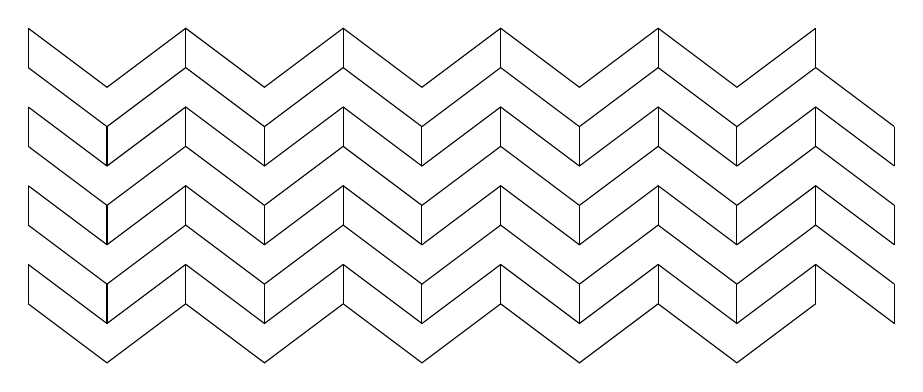
\begin{tikzpicture}[scale=1]


\draw  (0,0) -- (1,-0.75) -- (2,0) -- (3,-0.75) -- (4, 0) -- (5,-0.75)-- (6, 0) -- (7,-0.75)-- (8, 0) -- (9,-0.75)-- (10, 0);
\draw  (0,0.5) -- (1,-0.25) -- (2,0.5) -- (3,-0.25) -- (4, 0.5) -- (5,-0.25)-- (6, 0.5) -- (7,-0.25)-- (8, 0.5) -- (9,-0.25)-- (10, 0.5) -- (11,-0.25);
\draw  (0,1) -- (1,0.25) -- (2,1) -- (3,0.25) -- (4, 1) -- (5,0.25)-- (6, 1) -- (7,0.25)-- (8, 1) -- (9,0.25)-- (10, 1) -- (11,0.25);
\draw  (0,1.5) -- (1,0.75) -- (2,1.5) -- (3,0.75) -- (4, 1.5) -- (5,0.75)-- (6, 1.5) -- (7,0.75)-- (8, 1.5) -- (9,0.75)-- (10, 1.5) -- (11,0.75);
\draw  (0,2) -- (1,1.25) -- (2,2) -- (3,1.25) -- (4, 2) -- (5,1.25)-- (6, 2) -- (7,1.25)-- (8, 2) -- (9,1.25)-- (10, 2) -- (11,1.25);
\draw  (0,2.5) -- (1,1.75) -- (2,2.5) -- (3,1.75) -- (4, 2.5) -- (5,1.75)-- (6, 2.5) -- (7,1.75)-- (8, 2.5) -- (9,1.75)-- (10, 2.5) -- (11,1.75);
\draw  (0,3) -- (1,2.25) -- (2,3) -- (3,2.25) -- (4, 3) -- (5,2.25)-- (6, 3) -- (7,2.25)-- (8, 3) -- (9,2.25)-- (10, 3) -- (11,2.25);
\draw  (0,3.5) -- (1,2.75) -- (2,3.5) -- (3,2.75) -- (4, 3.5) -- (5,2.75)-- (6, 3.5) -- (7,2.75)-- (8,3.5) -- (9,2.75)-- (10, 3.5);


\draw (0,0) -- (0,0.5)   (0,1) -- (0,1.5)  (0,2) -- (0,2.5)  (0,3) -- (0,3.5);
\draw (2,0) -- (2,0.5)   (2,1) -- (2,1.5)  (2,2) -- (2,2.5)  (2,3) -- (2,3.5);
\draw (4,0) -- (4,0.5)   (4,1) -- (4,1.5)  (4,2) -- (4,2.5)  (4,3) -- (4,3.5);
\draw (6,0) -- (6,0.5)   (6,1) -- (6,1.5)  (6,2) -- (6,2.5)  (6,3) -- (6,3.5);
\draw (8,0) -- (8,0.5)   (8,1) -- (8,1.5)  (8,2) -- (8,2.5)  (8,3) -- (8,3.5);
\draw (10,0) -- (10,0.5)   (10,1) -- (10,1.5)  (10,2) -- (10,2.5)  (10,3) -- (10,3.5);

\draw (1,-0.25)  -- (1,0.25)  (1,0.75) -- (1,1.25) (1,1.75) -- (1,2.25);
\draw (3,-0.25) --  (3,0.25)  (3,0.75) -- (3,1.25) (3,1.75) -- (3,2.25);
\draw (5,-0.25)  -- (5,0.25)  (5,0.75) --  (5,1.25)  (5,1.75) -- (5,2.25);
\draw (7,-0.25) --  (7,0.25) (7,0.75)  --(7,1.25) (7,1.75) -- (7,2.25);
\draw (9,-0.25)  -- (9,0.25) (9,0.75) -- (9,1.25) (9,1.75)  --(9,2.25);
\draw (11,-0.25)  -- (11,0.25) (11,0.75) -- (11,1.25)  (11,1.75) -- (11,2.25);




\end{tikzpicture}
\end{center}
\caption{A wallpaper pattern in ${\mathbb R}^2$}
\label{Wallpaper}
\end{figure}
 
 
 
\subsection*{The Wallpaper Groups}
 
 
 
Suppose that we wish to study wallpaper patterns in the plane or
crystals in three dimensions. Wallpaper patterns are simply repeating
patterns in the plane (Figure~\ref{Wallpaper}). The analogs of
wallpaper patterns in ${\mathbb R}^3$ are crystals, which we can think of
as repeating patterns of molecules in three dimensions
(Figure~\ref{Crystals}). The mathematical equivalent of a wallpaper or
crystal pattern is called a  lattice. 
 
 
 
\begin{figure}[hbt]


%Replaced figure with tikz figure - TWJ 6/11/2010
\begin{center}
\tikzpreface{matrix_crystal_R3}
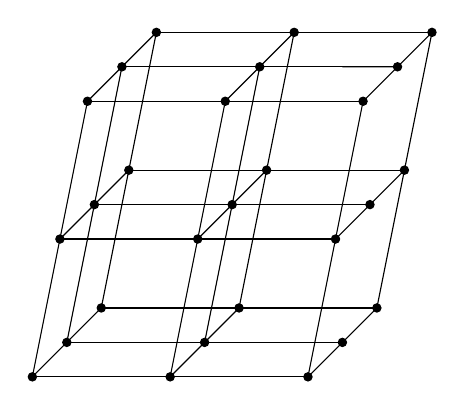
\begin{tikzpicture}[scale=1.75]


\draw  (0,0) -- (2,0)  (0.25,0.25) -- (2.25,0.25)  (0.5,0.5) -- (2.5,0.5);

\foreach \x in {0,1,2} \filldraw[fill=black, draw=black] (\x,0) circle (0.03);
\foreach \x in {0.25,1.25,2.25} \filldraw[fill=black, draw=black] (\x,0.25) circle (0.03);
\foreach \x in {0.5,1.5,2.5} \filldraw[fill=black, draw=black] (\x,0.5) circle (0.03);

\draw  (0.2,1) -- (2.2,1)  (0.45,1.25) -- (2.45,1.25)  (0.7,1.5) -- (2.7,1.5) ;

\foreach \x in {0.2,1.2,2.2} \filldraw[fill=black, draw=black] (\x,1) circle (0.03);
\foreach \x in {0.45,1.45,2.45} \filldraw[fill=black, draw=black] (\x,1.25) circle (0.03);
\foreach \x in {0.7,1.7,2.7} \filldraw[fill=black, draw=black] (\x,1.5) circle (0.03);

\draw  (0.4,2) -- (2.4,2)  (0.65,2.25) -- (2.65,2.25)  (0.9,2.5) -- (2.9,2.5) ;

\foreach \x in {0.4,1.4,2.4} \filldraw[fill=black, draw=black] (\x,2) circle (0.03);
\foreach \x in {0.65,1.65,2.65} \filldraw[fill=black, draw=black] (\x,2.25) circle (0.03);
\foreach \x in {0.9,1.9,2.9} \filldraw[fill=black, draw=black] (\x,2.5) circle (0.03);

\draw (0,0) -- (0.4,2)  (0.25,0.25) -- (0.65,2.25) (0.5,0.5) -- (0.9,2.5);
\draw (1,0) -- (1.4,2)  (1.25,0.25) -- (1.65,2.25) (1.5,0.5) -- (1.9,2.5);
\draw (2,0) -- (2.4,2)  (2.25,2.25) -- (2.65,2.25) (2.5,0.5) -- (2.9,2.5);

\draw (0,0) -- (0.5,0.5)  (1,0) -- (1.5,0.5)  (2,0) -- (2.5,0.5);

\draw  (0.2,1) -- (0.7,1.5)  (1.2,1) -- (1.7,1.5)  (2.2,1) -- (2.7,1.5);

\draw  (0.4,2) -- (0.9,2.5) (1.4,2) -- (1.9,2.5)   (2.4,2) -- (2.9,2.5);


\end{tikzpicture}
\end{center}
\caption{A crystal structure in ${\mathbb R}^3$}
\label{Crystals}
\end{figure}
 
 

Let us examine wallpaper patterns in the plane a
little more closely. Suppose that ${\mathbf x}$ and ${\mathbf y}$ are
linearly independent vectors in ${\mathbb R}^2$; that is, one vector
cannot be a scalar multiple of the other. A \boldemph{
lattice}\index{Lattice of points} of ${\mathbf x}$ and ${\mathbf y}$ is
the set of all linear combinations $m {\mathbf x} + n {\mathbf y}$, where
$m$ and $n$ are integers. The vectors ${\mathbf x}$ and ${\mathbf y}$ are
said to be a \boldemph{basis}\index{Basis of a lattice} for the lattice.
 
 
\begin{figure}[htb]


%Replaced figure with tikz figure - TWJ 6/11/2010
\begin{center}
\tikzpreface{matrix_lattice_R2}
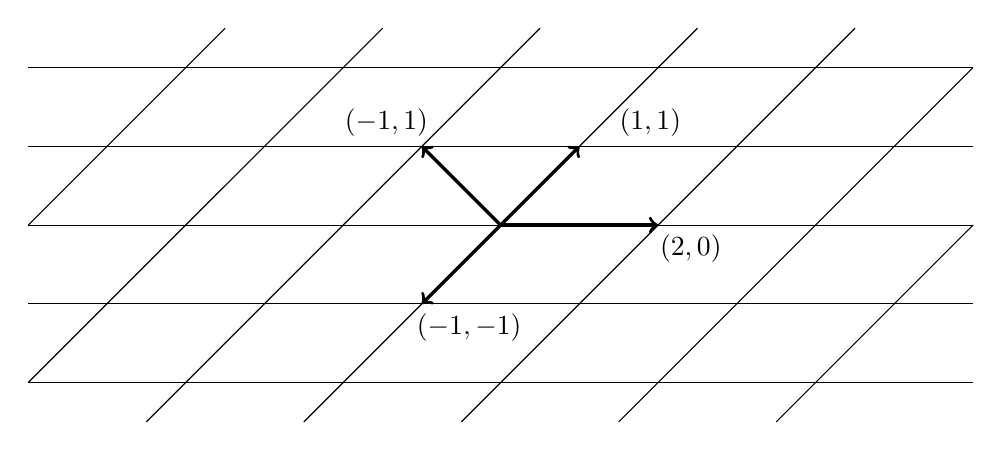
\begin{tikzpicture}[scale=1]



\foreach \x in {-2, -1, 0, 1, 2} \draw  (-6,\x) -- (6,\x); 

\draw (3.5,-2.5) -- (6,0);
\draw (1.5,-2.5) -- (6,2);
\draw (-0.5,-2.5) -- (4.5,2.5);
\draw (-2.5,-2.5) -- (2.5,2.5);
\draw (-4.5,-2.5) -- (0.5,2.5);
\draw (-6,-2) -- (-1.5,2.5);
\draw (-6,0) -- (-3.5,2.5);

\draw [->, very thick, black]  (0,0) -- (2,0);
\draw [->, very thick, black]  (0,0) -- (1,1);
\draw [->, very thick, black]  (0,0) -- (-1,1);
\draw [->, very thick, black]  (0,0) -- (-1,-1); 

\node [right] at (1.9,-0.3) {$(2,0)$};
\node [above] at (1.9,1) {$(1,1)$};
\node [above] at (-1.45,1) {$(-1,1)$};
\node [below] at (-0.4,-1) {$(-1,-1)$};

\end{tikzpicture}
\end{center}
\caption{A lattice in  ${\mathbb R}^2$}
\label{lattice}
\end{figure}
 
 
Notice that a lattice can have several bases. For example, the vectors
$(1,1)^{\rm t}$ and $(2,0)^{\rm t}$ have the  same lattice as the
vectors $(-1, 1)^{\rm t}$ and $(-1, -1)^{\rm t}$
(Figure~\ref{lattice}). However, any lattice is completely determined
by a basis. Given two bases for the same lattice, say $\{ {\mathbf x}_1,
{\mathbf x}_2 \}$ and $\{ {\mathbf y}_1, {\mathbf y}_2 \}$, we can write 
\begin{align*}
{\mathbf y}_1 & = \alpha_1  {\mathbf x}_1 + \alpha_2 {\mathbf x}_2 \\
{\mathbf y}_2 & = \beta_1  {\mathbf x}_1 + \beta_2 {\mathbf x}_2,
\end{align*}
where $\alpha_1$, $\alpha_2$, $\beta_1$, and $\beta_2$ are integers.
The matrix corresponding to this transformation is 
\[
U
=
\begin{pmatrix}
\alpha_1 & \alpha_2 \\
\beta_1 & \beta_2
\end{pmatrix}.
\]
If we wish to give ${\mathbf x}_1$ and ${\mathbf x}_2$ in terms of ${\mathbf
y}_1$ and ${\mathbf y}_2$, we need only calculate $U^{-1}$; that is, 
\[
U^{-1}
\begin{pmatrix}
{\mathbf y}_1 \\ {\mathbf y}_2
\end{pmatrix}
=
\begin{pmatrix}
{\mathbf x}_1 \\ {\mathbf x}_2
\end{pmatrix}.
\]
Since $U$ has integer entries, $U^{-1}$ must also have integer
entries; hence the determinants of both $U$ and $U^{-1}$ must be
integers. Because $U U^{-1} = I$,  
\[
\det(U U^{-1}) =\det(U) \det( U^{-1}) = 1;
\]
consequently, $\det(U) = \pm 1$. A matrix with determinant $\pm 1$ and
integer entries is called \boldemph{unimodular}\index{Matrix!unimodular}.
For example, the matrix 
\[
\begin{pmatrix}
3 & 1 \\
5 & 2
\end{pmatrix}
\]
is unimodular. It should be clear that there is a minimum length for
vectors in a lattice.  
 
 
We can classify lattices by studying their symmetry groups. The
symmetry group of a lattice is the subgroup of $E(2)$ that maps the
lattice to itself. We consider two lattices in ${\mathbb R}^2$ to be
equivalent if they have the same symmetry group.  Similarly,
classification of crystals in ${\mathbb R}^3$ is accomplished by
associating a symmetry group, called a \boldemph{space group}, with each
type of crystal\index{Group!space}. Two lattices are considered
different if their space groups are not the same.  The natural
question that now arises is how many space groups exist. 
 
 
A space group is composed of two parts: a \boldemph{translation
subgroup}\index{Subgroup!translation} and a \boldemph{point
group}\index{Group!point}.  The translation subgroup is an infinite
abelian subgroup of the space group made up of the translational
symmetries of the crystal; the point group is a finite group 
consisting  of rotations and reflections of the crystal about a point.
More specifically, a space group is a subgroup of $G \subset E(2)$
whose translations are a set of the form $\{ (I, t) : t \in L \}$,
where $L$ is a lattice. Space groups are, of course, infinite. Using
geometric arguments, we can prove the following theorem (see [5] or [6]).
 
 
 
 
\begin{theorem}
Every translation group in ${\mathbb R}^2$ is isomorphic to ${\mathbb Z}
\times {\mathbb Z}$.
\end{theorem}
 
 
\begin{figure}[bht]

\begin{center}
\tikzpreface{matrix_lattices_R2}
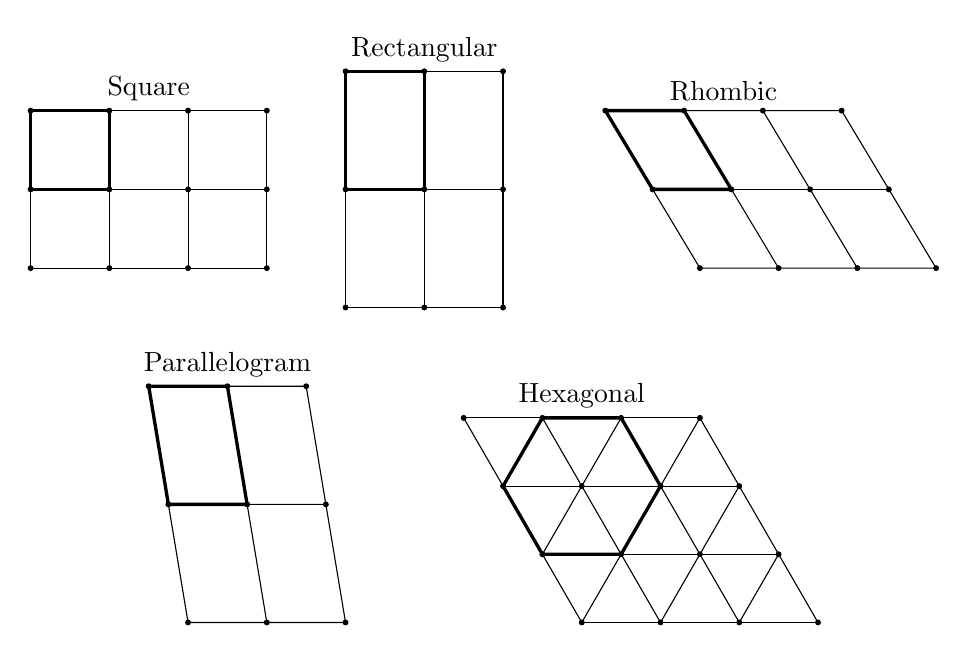
\begin{tikzpicture}[scale=1] %Replaced figure with tikz figure - TWJ 6/14/2010

\node [above] at (0,7) {Rectangular};
\draw (-1,4) -- (1,4) -- (1,7) -- (-1,7) -- cycle;
\draw  (0,4) -- (0,7)  (-1,5.5) -- (1,5.5);
\draw [very thick] (-1,5.5) -- (-1,7) -- (0,7) -- (0,5.5) -- cycle;
\foreach \x in {-1,0,1} \filldraw[fill=black, draw=black] (\x,4) circle (0.03);
\foreach \x in {-1,0,1} \filldraw[fill=black, draw=black] (\x,5.5) circle (0.03);
\foreach \x in {-1,0,1} \filldraw[fill=black, draw=black] (\x,7) circle (0.03);

\node [above] at (-3.5,6.5) {Square};
\draw (-2,4.5) -- (-5,4.5) -- (-5,6.5) -- (-2,6.5) -- cycle;
\draw  (-2,5.5) -- (-5,5.5)  (-3,4.5) -- (-3,6.5) (-4,4.5) -- (-4,6.5);
\draw [very thick] (-5,5.5) -- (-5,6.5) -- (-4,6.5) -- (-4,5.5) -- cycle;
\foreach \x in {-2, -3, -4, -5} \filldraw[fill=black, draw=black] (\x,4.5) circle (0.03);
\foreach \x in {-2, -3, -4, -5} \filldraw[fill=black, draw=black] (\x,5.5) circle (0.03);
\foreach \x in {-2, -3, -4, -5} \filldraw[fill=black, draw=black] (\x,6.5) circle (0.03);

\node [above] at (3.8,6.5) {Rhombic};
\draw (3.5,4.5)   -- (6.5,4.5) -- (5.3,6.5) -- (2.3,6.5) -- cycle;
\draw (2.9,5.5) -- (5.9,5.5);
\draw (4.5,4.5) -- (3.3,6.5);
\draw  (5.5,4.5) -- (4.3,6.5);
\draw [very thick] (2.3,6.5) -- (3.3,6.5) -- (3.9,5.5) -- (2.9,5.5) -- cycle;
\foreach \x in {3.5,4.5,5.5,6.5} \filldraw[fill=black, draw=black] (\x,4.5) circle (0.03);
\foreach \x in {2.9,3.9,4.9,5.9} \filldraw[fill=black, draw=black] (\x,5.5) circle (0.03);
\foreach \x in {2.3,3.3,4.3,5.3} \filldraw[fill=black, draw=black] (\x,6.5) circle (0.03);

\node [above] at (-2.5,3) {Parallelogram};
\draw (-1,0) -- (-3,0) -- (-3.5,3) -- (-1.5,3) -- cycle;
\draw  (-2,0) -- (-2.5,3)  (-3.25,1.5) -- (-1.25,1.5);
\draw [very thick] (-3.25,1.5) -- (-3.5,3) -- (-2.5,3) -- (-2.25,1.5) -- cycle;
\foreach \x in {-1,-2,-3} \filldraw[fill=black, draw=black] (\x,0) circle (0.03);
\foreach \x in {-1.25,-2.25,-3.25} \filldraw[fill=black, draw=black] (\x,1.5) circle (0.03);
\foreach \x in {-1.5,-2.5,-3.5} \filldraw[fill=black, draw=black] (\x,3) circle (0.03);

\node [above] at (2,2.6) {Hexagonal}; %Couldn't figure out an elegant way to do the hexagonal lattice - TWJ 6/14/2010
\draw (2,0) -- (5,0);
\draw (1.5,0.866) -- (4.5,0.866);
\draw (1,1.732) -- (4,1.732);
\draw (0.5,2.598) -- (3.5,2.598);
\draw (2,0) -- (0.5,2.598);
\draw (3,0) -- (1.5,2.598);
\draw (4,0) -- (2.5,2.598);
\draw (5,0) -- (3.5,2.598);
\draw (2,0) -- (3.5,2.598);
\draw (3,0) -- (4,1.732);
\draw (4,0) -- (4.5,0.866);
\draw (1.5,0.866) -- (2.5,2.598);
\draw (1,1.732) -- (1.5,2.598);
\draw [very thick] (1.5,0.866) -- (1,1.732) -- (1.5,2.598) -- (2.5,2.598) -- (3,1.732) --  (2.5,0.866) -- cycle;
\foreach \x in {2,3,4,5} \filldraw[fill=black, draw=black] (\x,0) circle (0.03);
\foreach \x in {1.5,2.5,3.5,4.5} \filldraw[fill=black, draw=black] (\x,0.866) circle (0.03);
\foreach \x in {1,2,3,4} \filldraw[fill=black, draw=black] (\x,1.732) circle (0.03);
\foreach \x in {0.5, 1.5,2.5,3.5} \filldraw[fill=black, draw=black] (\x,2.598) circle (0.03);

\end{tikzpicture}
\end{center}
\caption{Types of lattices in  ${\mathbb R}^2$}
\label{Types}
\end{figure}
 
 
The point group of $G$ is $G_0 = \{A : (A,b) \in G \text{ for some }
b \}$. In particular, $G_0$ must be a subgroup of $O(2)$. Suppose
that ${\mathbf x}$ is a vector in a lattice $L$ with space group $G$,
translation group $H$, and point group $G_0$. For any element $(A,
{\mathbf y})$ in $G$,   
\begin{align*}
(A, {\mathbf y}) (I, {\mathbf x}) (A, {\mathbf y})^{-1}
& =
(A,A {\mathbf x} + {\mathbf y}) (A^{-1},-A^{-1} {\mathbf y}) \\
& =
(A A^{-1},-A A^{-1} {\mathbf y} + A {\mathbf x} + {\mathbf y}) \\
& =
(I, A {\mathbf x});
\end{align*}
hence, $(I, A {\mathbf x})$ is in the translation group of $G$. More
specifically, $A {\mathbf x}$ must be in the lattice $L$. It is
important to note that $G_0$ is not usually a subgroup of the space
group $G$; however, if $T$ is the translation subgroup of $G$, then
$G/T \cong G_0$. The proof of the following theorem can be found in
[2], [5], or~[6].
 
 
 
\begin{theorem}
The point group in the wallpaper groups is isomorphic to ${\mathbb Z}_n$
or $D_n$, where $n = 1, 2, 3, 4, 6$. 
\end{theorem}
 
 
To answer the question of how the point groups and the translation
groups can be combined, we must look at the different types of
lattices. Lattices can be classified by the structure of a single
lattice cell. The possible cell shapes are parallelogram, rectangular,
square, rhombic, and hexagonal (Figure~\ref{Types}). The wallpaper
groups can now be classified according to the types of reflections
that occur in each group: these are ordinarily reflections, glide
reflections, both, or none.
 
 
 
\begin{table}[htb]
\caption{The 17 wallpaper groups}{\small
\begin{center}
\begin{tabular}{|l|l|l|l|}
\hline
Notation and &             &              & Reflections  \\
Space Groups & Point Group & Lattice Type & or Glide Reflections? \\
\hline
p1 & ${\mathbb Z}_1$ & parallelogram & none \\
p2 & ${\mathbb Z}_2$ & parallelogram & none \\
p3 & ${\mathbb Z}_3$ & hexagonal & none \\
p4 & ${\mathbb Z}_4$ & square & none \\
p6 & ${\mathbb Z}_6$ & hexagonal & none \\
pm & $D_1$ & rectangular & reflections \\
pg & $D_1$ & rectangular & glide reflections\\
cm & $D_1$ & rhombic & both \\
pmm & $D_2$ & rectangular & reflections \\
pmg & $D_2$ & rectangular & glide reflections \\
pgg & $D_2$ & rectangular & both \\
c2mm & $D_2$ & rhombic & both \\
p3m1, p31m & $D_3$ & hexagonal & both \\
p4m, p4g & $D_4$ & square & both \\
p6m & $D_6$ & hexagonal & both \\
\hline
\end{tabular} \label{table:wallpaper}
\end{center}
}
\end{table}
 
 
\begin{theorem}
There are exactly 17 wallpaper groups.
\end{theorem}
 
 
\begin{figure}[htb]


\begin{center}
\tikzpreface{matrix_p4m_p4g}
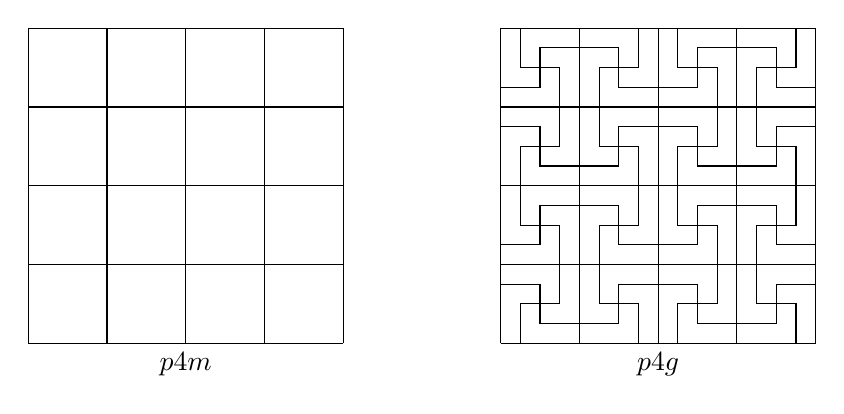
\begin{tikzpicture}[scale=1] %Replaced figure with tikz figure - TWJ 6/14/2010

\draw[step=1] (-5,0) grid (-1,4);
\node [below] at (-3,0) {$p4m$};

\draw[step=1] (1,0) grid (5,4);
\node [below] at (3,0) {$p4g$};
\draw (1.25,0) -- (1.25,0.5) -- (1.75,0.5) -- (1.75,1.5) -- (1.25,1.5) -- (1.25,2.5) -- (1.75,2.5) -- (1.75,3.5) -- (1.25,3.5) -- (1.25,4);
\draw  (2.75,0) -- (2.75,0.5) -- (2.25,0.5) -- (2.25,1.5) -- (2.75,1.5) -- (2.75,2.5) -- (2.25,2.5) -- (2.25,3.5) -- (2.75,3.5) -- (2.75,4);
\draw   (3.25,0) -- (3.25,0.5) -- (3.75,0.5) -- (3.75,1.5) -- (3.25,1.5) -- (3.25,2.5) -- (3.75,2.5) -- (3.75,3.5) -- (3.25,3.5) -- (3.25,4);
\draw   (4.75,0) -- (4.75,0.5) -- (4.25,0.5) -- (4.25,1.5) -- (4.75,1.5) -- (4.75,2.5) -- (4.25,2.5) -- (4.25,3.5) -- (4.75,3.5) -- (4.75,4);

\draw  (1,0.75) -- (1.5,0.75) -- (1.5,0.25) -- (2.5,0.25) -- (2.5,0.75) -- (3.5,0.75) -- (3.5,0.25) -- (4.5,0.25) -- (4.5,0.75) -- (5, 0.75);
\draw  (1,1.25) -- (1.5,1.25) -- (1.5,1.75) -- (2.5,1.75) -- (2.5,1.25) -- (3.5,1.25) -- (3.5,1.75) -- (4.5,1.75) -- (4.5,1.25) -- (5, 1.25);

\draw  (1,2.75) -- (1.5,2.75) -- (1.5,2.25) -- (2.5,2.25) -- (2.5,2.75) -- (3.5,2.75) -- (3.5,2.25) -- (4.5,2.25) -- (4.5,2.75) -- (5, 2.75);
\draw (1,3.25) -- (1.5,3.25) -- (1.5,3.75) -- (2.5,3.75) -- (2.5,3.25) -- (3.5,3.25) -- (3.5,3.75) -- (4.5,3.75) -- (4.5,3.25) -- (5, 3.25);


\end{tikzpicture}
\end{center}
\caption{The wallpaper groups p4m and  p4g}
\label{p4m}
\end{figure}
 
 
 
The 17 wallpaper groups are listed in Table~\ref{table:wallpaper}. The groups p3m1 and
p31m can be distinguished by whether or not all of their threefold
centers lie on the reflection axes: those of p3m1 must, whereas those
of p31m may not. Similarly, the fourfold centers of p4m must lie on
the reflection axes whereas those of p4g need not (Figure~\ref{p4m}).
The complete proof of this theorem can be found in several of the
references at the end of this chapter, including [5], [6], [10],
and~[11]. 
 
 
 
\histhead
 
 
\noindent{\small \histf
Symmetry groups have intrigued mathematicians for a long time.
Leonardo da Vinci was probably the first person to know all of the
point groups.  At the International Congress of Mathematicians in
1900, David Hilbert\index{Hilbert, David} gave a now-famous address
outlining 23 problems to guide mathematics in the twentieth
century.  Hilbert's eighteenth problem asked whether or not
crystallographic groups in $n$ dimensions were always finite.  In
1910, L.~Bieberbach\index{Bieberbach, L.} proved that crystallographic
groups are finite in every dimension.  Finding out how many of these
groups there are in each dimension is another matter. In ${\mathbb R}^3$
there are 230 different space groups; in ${\mathbb R}^4$ there are 4783.
No one has been able to compute the number of space groups for ${\mathbb
R}^5$ and beyond. It is interesting to note that the crystallographic
groups were found mathematically for ${\mathbb R}^3$ before the 230
different types of crystals were actually discovered in nature.
\histbox
}
 
 
 
\markright{EXERCISES}
\section*{Exercises}
\exrule
 
 
{\small
\begin{enumerate}
 
 
 
\item
Prove the identity
\[
\langle {\mathbf x}, {\mathbf y} \rangle = \frac{1}{2}
\left[
\|{\mathbf x} + {\mathbf y}\|^2 - \|{\mathbf x}\|^2 - \| {\mathbf y}\|^2
\right].
\]
 
 
\item
Show that $O(n)$ is a group.
 
 
\item
Prove that the following matrices are orthogonal. Are any of
these matrices in $SO(n)$?
\begin{multicols}{2}
\begin{enumerate}

\item
\[
\begin{pmatrix}
1/\sqrt{2} & -1/\sqrt{2} \\
1/\sqrt{2} & 1/\sqrt{2}
\end{pmatrix}
\]

\item
\[
\begin{pmatrix}
1 / \sqrt{5} & 2 / \sqrt{5} \\
- 2 /\sqrt{5} & 1/ \sqrt{5}
\end{pmatrix}
\]

\item
\[
\begin{pmatrix}
4/ \sqrt{5} & 0 & 3 / \sqrt{5} \\
-3 / \sqrt{5} & 0 & 4 / \sqrt{5} \\
0 & -1 & 0
\end{pmatrix}
\]

\item
\[
\begin{pmatrix}
1/3 & 2/3 & - 2/3 \\
- 2/3 & 2/3 & 1/3 \\
-2/3 & 1/3 & 2/3
\end{pmatrix}
\]


\end{enumerate}
\end{multicols}
 

 
\item %%%%%%%%%%%%%%%%%%%%%%
Determine the symmetry group of each of the figures in
Figure~\ref{Determine}. 
\begin{figure}[htb]

\begin{center}
\tikzpreface{matrix_group_exercise}
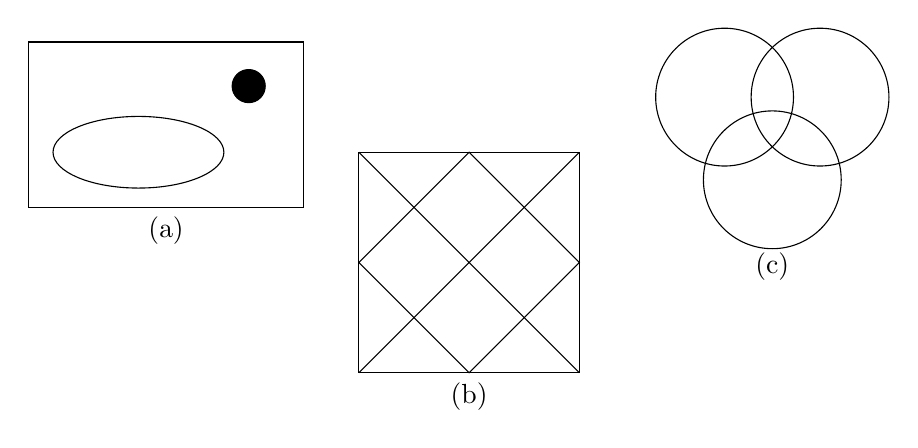
\begin{tikzpicture}[scale=0.7] %Replaced figure with tikz figure - TWJ 6/14/2010

\draw (-2,0) -- (2,0) -- (2,4) -- (-2,4) -- cycle;
\draw (0,0) -- (2,2) -- (0,4) -- (-2,2) -- cycle;
\draw (-2,0) -- (2,4) (2,0) -- (-2,4);
\node [below] at (0,0) {(b)};

\draw (-3,3) -- (-8,3) -- (-8,6) -- (-3,6) -- cycle;
\draw (-6,4) ellipse (1.55 and 0.65);
\filldraw[fill=black, draw=black] (-4,5.2) circle (0.3);
\node [below] at (-5.5,3) {(a)};



\draw (5.5,4.5)  +(270:1) circle (1.25);
\draw (5.5,4.5)  +(30:1) circle (1.25);
\draw (5.5,4.5)  +(150:1) circle (1.25);
\node [below] at (5.5,2.35) {(c)};


\end{tikzpicture}
\end{center}
\caption{}
\label{Determine}
\end{figure}
 
 
\item
Let ${\mathbf x}$, ${\mathbf y}$, and ${\mathbf w}$ be vectors in ${\mathbb
R}^n$ and $\alpha \in {\mathbb R}$.  Prove each of the following
properties of inner products.
\begin{enumerate}
 
 \item
$\langle {\mathbf x}, {\mathbf y} \rangle = \langle {\mathbf y}, {\mathbf x}
\rangle$. 
 
 \item
$\langle {\mathbf x}, {\mathbf y} + {\mathbf w} \rangle = \langle
{\mathbf x}, {\mathbf y} \rangle + \langle {\mathbf x}, {\mathbf w}
\rangle$.
 
 \item
$\langle \alpha {\mathbf x}, {\mathbf y} \rangle = \langle
{\mathbf x}, \alpha {\mathbf y} \rangle = \alpha \langle  {\mathbf
x}, {\mathbf y} \rangle$.
 
 \item
$\langle {\mathbf x}, {\mathbf x} \rangle \geq 0$ with equality exactly
when ${\mathbf x} = 0$. 
 
 \item
If $\langle {\mathbf x}, {\mathbf y} \rangle = 0$  for all ${\mathbf x}$ in
${\mathbb R}^n$, then ${\mathbf y} = 0$. 
 
\end{enumerate}
 
 
\item \label{matrix:En_group_exercise}
Verify that
\[
E(n)
=
\{(A, {\mathbf x}) : A \in O(n) \mbox{ and } {\mathbf x} \in
{\mathbb R}^n \}
\]
is a group.
 
 
\item
Prove that $\{ (2,1), (1,1) \}$  and $\{ ( 12, 5), ( 7, 3) \}$ are bases
for the same lattice. 
 
 
\item
Let $G$ be a subgroup of $E(2)$ and suppose that $T$ is the
translation subgroup of $G$.  Prove that the point group of $G$ is
isomorphic to $G/T$. 
 
 
\item
Let $A \in SL_2({\mathbb R})$ and suppose that the vectors ${\mathbf x}$
and ${\mathbf y}$ form two sides of a parallelogram in ${\mathbb R}^2$.
Prove that the area of this parallelogram is the same as the area of
the parallelogram with sides $A{\mathbf x}$ and $A{\mathbf y}$. 
 
 
\item
Prove that $SO(n)$ is a normal subgroup of $O(n)$.
 
 
\item
Show that any isometry $f$ in ${\mathbb R}^n$ is a one-to-one map.
 
 
\item
Show that an element in $E(2)$ of the form $(A, {\mathbf x})$,
where ${\mathbf x} \neq 0$, has infinite order.
 
 
\item
Prove or disprove: There exists an infinite abelian subgroup of 
$O(n)$.
 
 
\item
Let ${\mathbf x} = (x_1, x_2)$ be a point on the unit circle in ${\mathbb
R}^2$; that is, $x_1^2 + x_2^2 = 1$. If $A \in O(2)$, show that $A
{\mathbf x}$ is also a point on the unit circle. 
 
 
 
\item
Let $G$ be a group with a subgroup $H$ (not necessarily normal) and a
normal subgroup $N$. Then $G$ is a \boldemph{semidirect
product}\index{Semidirect product} of $N$ by $H$ if  
\begin{itemize}
 
 \item
$H \cap N = \{ id \}$;
 
 \item
$HN=G$.
 
\end{itemize}
Show that each of the following is true.
\begin{enumerate}
 
 \item
$S_3$ is the semidirect product of $A_3$ by $H = \{(1), (12) \}$.
 
 \item
The quaternion group, $Q_8$, cannot be written as a semidirect product. 
 
 \item
$E(2)$ is the semidirect product of $O(2)$ by $H$, where $H$ consists
of all translations in ${\mathbb R}^2$. 
 
\end{enumerate}
 
 
 
\item
Determine which of the 17 wallpaper groups preserves the symmetry of
the pattern in Figure~\ref{Wallpaper}.  
 
\begin{figure}[htb]

\begin{center}
\tikzpreface{matrix_wallpaper_exercise}
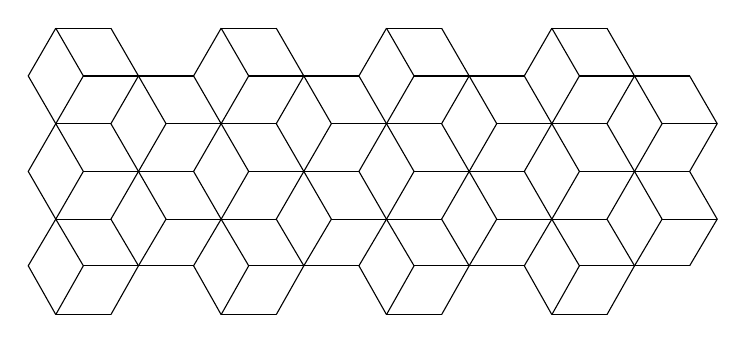
\begin{tikzpicture}[scale=0.7] %Replaced figure with tikz figure - TWJ 6/14/2010

\draw (0.5,0) -- (1.5,0)  (3.5,0) -- (4.5,0) (6.5,0) -- (7.5,0) (9.5,0) -- (10.5,0);
\draw (1,0.886) -- (3,0.886) (4,0.886) -- (6,0.886) (7,0.886) -- (9,0.886) (10,0.886) -- (12,0.886);
\draw (0.5,1.732) -- (1.5,1.732)  (2.5,1.732) -- (4.5,1.732) (5.5,1.732) -- (7.5,1.732) (8.5,1.732) -- (10.5,1.732) (11.5,1.732) -- (12.5,1.732);
\draw (1,2.598) -- (3,2.598) (4,2.598) -- (6,2.598) (7,2.598) -- (9,2.598) (10,2.598) -- (12,2.598);
\draw (0.5,3.464) -- (1.5,3.464)  (2.5,3.464) -- (4.5,3.464) (5.5,3.464) -- (7.5,3.464) (8.5,3.464) -- (10.5,3.464) (11.5,3.464) -- (12.5,3.464);
\draw (1,4.33) -- (3,4.33) (4,4.33) -- (6,4.33) (7,4.33) -- (9,4.33) (10,4.33) -- (12,4.33);
\draw (0.5,5.196) -- (1.5,5.196)  (3.5,5.196) -- (4.5,5.196) (6.5,5.196) -- (7.5,5.196) (9.5,5.196) -- (10.5,5.196);

\draw (0.5,0) -- (0,0.886) -- (0.5,1.732) -- (0,2.598) -- (0.5,3.464) -- (0,4.33) -- (0.5,5.196);
\draw (0.5,0) -- (1,0.886) -- (0.5,1.732) -- (1,2.598) -- (0.5,3.464) -- (1,4.33) -- (0.5,5.196);
\draw (1.5,0) -- (2,0.886) -- (1.5,1.732) -- (2,2.598) -- (1.5,3.464) -- (2,4.33) -- (1.5,5.196);
\draw (2,0.886) -- (2.5,1.732) -- (2,2.598) -- (2.5,3.464) -- (2,4.33);
\draw (3,0.886) -- (3.5,1.732) -- (3,2.598) -- (3.5,3.464) -- (3,4.33);
\draw (3.5,0) -- (3,0.886) (3,4.33) -- (3.5,5.196);
\draw (3.5,0) -- (4,0.886) -- (3.5,1.732) -- (4,2.598) -- (3.5,3.464) -- (4,4.33) -- (3.5,5.196);
\draw (4.5,0) -- (5,0.886) -- (4.5,1.732) -- (5,2.598) -- (4.5,3.464) -- (5,4.33) -- (4.5,5.196);
\draw (5,0.886) -- (5.5,1.732) -- (5,2.598) -- (5.5,3.464) -- (5,4.33);
\draw (6.5,0) -- (6,0.886) -- (6.5,1.732) -- (6,2.598) -- (6.5,3.464) -- (6,4.33) -- (6.5,5.196);
\draw (6.5,0) -- (7,0.886) -- (6.5,1.732) -- (7,2.598) -- (6.5,3.464) -- (7,4.33) -- (6.5,5.196);
\draw (7.5,0) -- (8,0.886) -- (7.5,1.732) -- (8,2.598) -- (7.5,3.464) -- (8,4.33) -- (7.5,5.196);
\draw (8,0.886) -- (8.5,1.732) -- (8,2.598) -- (8.5,3.464) -- (8,4.33);
\draw (9.5,0) -- (9,0.886) -- (9.5,1.732) -- (9,2.598) -- (9.5,3.464) -- (9,4.33) -- (9.5,5.196);
\draw (9.5,0) -- (10,0.886) -- (9.5,1.732) -- (10,2.598) -- (9.5,3.464) -- (10,4.33) -- (9.5,5.196);
\draw (10.5,0) -- (11,0.886) -- (10.5,1.732) -- (11,2.598) -- (10.5,3.464) -- (11,4.33) -- (10.5,5.196);
\draw (11,0.886) -- (11.5,1.732) -- (11,2.598) -- (11.5,3.464) -- (11,4.33);
\draw (12,0.886) -- (12.5,1.732) -- (12,2.598) -- (12.5,3.464) -- (12,4.33);



\end{tikzpicture}
\end{center}
\caption{}
\label{For17}
\end{figure}
 
\item
Determine which of the 17 wallpaper groups preserves the symmetry of
the pattern in Figure~\ref{For17}.  
 
 
 
\item
Find the rotation group of a dodecahedron.
 
  
 
\item
For each of the 17 wallpaper groups, draw a wallpaper pattern having
that group as a symmetry group.  
 
\end{enumerate}
}
 
 
 
\subsection*{References and Suggested Readings}
 
 
 
{\small
\begin{itemize} %%References checked -- TWJ 6/14/2010
 
\item[\textbf{[1]}]
Coxeter, H. M. and Moser, W. O. J. \textit{Generators and
Relations for Discrete Groups}, 3rd ed. Springer-Verlag, New
York, 1972.
 
\item[\textbf{[2]}]
Grove, L. C. and Benson, C. T. \textit{Finite Reflection
Groups}. 2nd ed. Springer-Verlag, New York, 1985.
 
\item[\textbf{[3]}]
Hiller, H. ``Crystallography and Cohomology of Groups,''
\textit{American Mathematical Monthly} \textbf{93} (1986), 765--79.
 
\item[\textbf{[4]}]
Lockwood, E. H. and Macmillan, R. H. \textit{Geometric
Symmetry}. Cambridge University Press, Cambridge, 1978.
 
\item[\textbf{[5]}]
Mackiw, G. \textit{Applications of Abstract Algebra}. Wiley,
New York, 1985.
 
 
\item[\textbf{[6]}]
Martin,  G.  \textit{Transformation  Groups:  An Introduction to
Symmetry}.  Springer-Verlag, New York, 1982.
 
  
\item[\textbf{[7]}]
Milnor, J. ``Hilbert's Problem 18: On Crystallographic
Groups, Fundamental Domains, and Sphere Packing,'' {\it
Proceedings of Symposia in Pure Mathematics} \textbf{18},
American Mathematical Society, 1976.
 
\item[\textbf{[8]}]
Phillips, F. C. \textit{An Introduction to Crystallography}.
4th ed. Wiley, New York, 1971.
 
\item[\textbf{[9]}]
Rose, B. I. and Stafford, R. D. ``An Elementary Course in
Mathematical Symmetry,'' \textit{American Mathematical Monthly} \textbf{
88} (1980), 54--64.
 
 
\item[\textbf{[10]}]
Schattschneider, D. ``The Plane Symmetry Groups: Their
Recognition and Their Notation,'' \textit{American Mathematical 
Monthly} \textbf{85} (1978), 439--50.
 
 
\item[\textbf{[11]}]
Schwarzenberger, R. L. ``The 17 Plane Symmetry Groups,'' {\it
Mathematical  Gazette} \textbf{58} (1974), 123--31. 
 
 
\item[\textbf{[12]}]
Weyl, H. \textit{Symmetry}. Princeton University Press, Princeton, NJ,
1952. 
 
 
\end{itemize}
}
 
 
 
 
   %Groups of Symmetries
%%%%(c)
%%%%(c)  This file is a portion of the source for the textbook
%%%%(c)
%%%%(c)    Abstract Algebra: Theory and Applications
%%%%(c)    by Thomas W. Judson
%%%%(c)
%%%%(c)    Sage Material
%%%%(c)    Copyright 2011 by Robert A. Beezer
%%%%(c)
%%%%(c)  See the file COPYING.txt for copying conditions
%%%%(c)
%%%%(c)
Sage is able to create direct products of cyclic groups, though they are realized as permutation groups.  This is a situation that should improve.  However, with a classification of finite abelian groups, we can describe how to construct in Sage every group of order less than 16.   %Abelian and Solvable Groups
%%%%(c)
%%%%(c)  This file is a portion of the source for the textbook
%%%%(c)
%%%%(c)    Abstract Algebra: Theory and Applications
%%%%(c)    by Thomas W. Judson
%%%%(c)
%%%%(c)    Sage Material
%%%%(c)    Copyright 2011 by Robert A. Beezer
%%%%(c)
%%%%(c)  See the file COPYING.txt for copying conditions
%%%%(c)
%%%%(c)
Sage has many commands related to conjugacy, which is a group action.  It also has commands for orbits and stabilizers of permutation groups.  In the supplement, we illustrate the automorphism group of a (combinatorial) graph as another example of a group action on the vertex set of the graph.  %Group Actions
%%%%(c)
%%%%(c)  This file is a portion of the source for the textbook
%%%%(c)
%%%%(c)    Abstract Algebra: Theory and Applications
%%%%(c)    by Thomas W. Judson
%%%%(c)
%%%%(c)    Sage Material
%%%%(c)    Copyright 2011 by Robert A. Beezer
%%%%(c)
%%%%(c)  See the file COPYING.txt for copying conditions
%%%%(c)
%%%%(c)
Sage will compute a single Sylow $p$-subgroup for each prime divisor $p$ of the order of the group.  Then, with conjugacy, all of the Sylow $p$-subgroups can be enumerated.  It is also possible to compute the normalizer of a subgroup.    %Sylow Theorems
%%%%(c)
%%%%(c)  This file is a portion of the source for the textbook
%%%%(c)
%%%%(c)    Abstract Algebra: Theory and Applications
%%%%(c)    by Thomas W. Judson
%%%%(c)
%%%%(c)    Sage Material
%%%%(c)    Copyright 2011 by Robert A. Beezer
%%%%(c)
%%%%(c)  See the file COPYING.txt for copying conditions
%%%%(c)
%%%%(c)
\begin{sageverbatim}\end{sageverbatim}
%
\sageexercise{1}%
Define the two rings ${\mathbb Z}_{11}$ and ${\mathbb Z}_{12}$ with the commands \verb?R = Integers(11)? and \verb?S = Integers(12)?.  For each ring, use the relevant command to determine:  if the ring is finite, if it is commutative, if it is an integral domain and if it is a field.  Then use single Sage commands to find the order of the ring, list the elements, and output the multiplicative identity (i.e.\ $1$, if it exists).
\begin{sageverbatim}\end{sageverbatim}
%
\sageexercise{2}%
Define \verb?R? to be the ring of integers, ${\mathbb Z}$, by executing \verb?R = ZZ? or \verb?R = Integers()?.  A command like \verb?R.ideal(4)? will create the principal ideal $\langle 4\rangle$.  The same command can accept more than one generator, so for example, \verb?R.ideal(3, 5)? will create the ideal $\{a\cdot 3+ b\cdot 5\mid a,b\in{\mathbb Z}\}$.  Create several ideals of ${\mathbb Z}$ with two generators and ask Sage to print each as you create it.  Explain what you observe and then create code that will test your observation for thousands of different examples.
\begin{sageverbatim}\end{sageverbatim}
%
\sageexercise{3}%
Create a finite field $F$ of order 81 with \verb?F.<t>=FiniteField(3^4)?.\\
(a) List the elements of $F$. \\
(b) Obtain the generators of $F$ with \verb?F.gens()?. \\
(c) Obtain the first generator of $F$ and save it as \verb?u? with \verb?u = F.0? (alternatively, \verb?u = F.gen(0)?). \\
(d) Compute the first 80 powers of \verb?u? and comment. \\
(e) The generator you have worked with above is a root of a polynomial over ${\mathbb Z}_3$.  Obtain this polynomial with \verb?F.modulus()? and use this observation to explain the entry in your list of powers that is the fourth power of the generator.
\begin{sageverbatim}\end{sageverbatim}
%
\sageexercise{4}%
Build and analyze a quotient ring as follows:\\
(a) Use \verb?P.<z>=(Integers(7))[]? to construct a ring $P$ of polynomials in $z$ with coefficients from ${\mathbb Z}_7$.\\
(b) Use \verb?K = P.ideal(z^2+z+3)? to build a principal ideal $K$ generated by the polynomial $z^2+z+3$.\\
(c) Use \verb?H = P.quotient(K)? to build $H$, the quotient ring of $P$ by $K$.\\
(d) Use Sage to verify that $H$ is a field. \\
(e) As in the previous exercise, obtain a generator and examine the proper collection of powers of that generator.
\begin{sageverbatim}\end{sageverbatim}
    %Introduction to Rings
%%%%(c)
%%%%(c)  This file is a portion of the source for the textbook
%%%%(c)
%%%%(c)    Abstract Algebra: Theory and Applications
%%%%(c)    by Thomas W. Judson
%%%%(c)
%%%%(c)    Sage Material
%%%%(c)    Copyright 2011 by Robert A. Beezer
%%%%(c)
%%%%(c)  See the file COPYING.txt for copying conditions
%%%%(c)
%%%%(c)
\begin{sageverbatim}\end{sageverbatim}
%
\sageexercise{1}%
Consider the polynomial $x^3-3x+4$.  Compute the most thorough factorization of this polynomial over each of the following fields:  (a) the finite field ${\mathbb Z}_5$, (b) a finite field with 125 elements, (c) the rationals, (d) the real numbers and (e) the complex numbers.  To do this, build the appropriate polynomial ring, and construct the polynomial as a member of this ring, and use the \verb?.factor()? method.
\begin{sageverbatim}\end{sageverbatim}
%
\sageexercise{2}%
``Conway polynomials'' are irreducible polynomials over ${\mathbb Z}_p$ that Sage (and other software) uses to build maximal ideals in polynomial rings, and thus quotient rings that are fields. Roughly speaking, they are ``canonical'' choices for each degree and each prime.  The command \verb?conway_polynomial(p, n)? will return a database entry that is an irreducible polynomial of degree $n$ over ${\mathbb Z}_p$.\par
%
Execute the command \verb?conway_polynomial(5, 4)? to obtain an allegedly irreducible polynomial of degree 4 over ${\mathbb Z}_5$:  $p = x^{4} + 4x^{2} + 4x + 2$.  First determine that p has no linear factors.  The only possibility left is that \verb?p? factors as two quadratic polynomials over ${\mathbb Z}_5$.  Use a list comprehension with \emph{three} \verb?for? statements to create \emph{every} possible quadratic polynomial over ${\mathbb Z}_5$.  Now use this list to create every possible product of two quadratic polynomials and check to see if \verb?p? is in this list.\par
%
More on Conway polynomials is available at
\url{http://www.math.rwth-aachen.de/~Frank.Luebeck/data/ConwayPol/index.html}
\begin{sageverbatim}\end{sageverbatim}
%
\sageexercise{3}%
Construct a finite field of order $729$ as a quotient of a polynomial ring by a principal ideal generated with a Conway polynomial.
\begin{sageverbatim}\end{sageverbatim}
%
\sageexercise{4}%
Define the polynomials $p = x^3 + 2x^2 + 2x + 4$ and $q = x^4 + 2x^2$ as polynomials with coefficients from the integers.  Compute \verb?gcd(p, q)? and verify that the result divides both \verb?p? and \verb?q? (just form a fraction in Sage and see that it simplifies cleanly, or use the \verb?.quo_rem()? method).\par
%
Proposition~\extref{poly:gcd_ther}{17.7}{existence of polynomial gcd} says there are polynomials $r(x)$ and $s(x)$ such that the greatest common divisor equals $r(x)p(x)+s(x)q(x)$, \emph{if the coefficients come from a field}.  Since here we have two polynomials over the integers, investigate the results returned by Sage for the extended gcd, \verb?xgcd(p, q)?.  In particular, show that the first result of the returned triple is a multiple of the gcd.  Then verify the ``linear combination'' property of the result.
\begin{sageverbatim}\end{sageverbatim}
%
\sageexercise{5}%
For a polynomial ring over a field, every ideal is principal.  Begin with the ring of polynomials over the rationals.  Experiment with constructing ideals using two generators and then see that Sage converts the ideal to a principal ideal with a single generator.  (You can get this generator with the ideal method \verb?.gen()?.)  Can you explain how this single generator is computed?
\begin{sageverbatim}\end{sageverbatim}
     %Polynomial Rings
%%%%(c)
%%%%(c)  This file is a portion of the source for the textbook
%%%%(c)
%%%%(c)    Abstract Algebra: Theory and Applications
%%%%(c)    by Thomas W. Judson
%%%%(c)
%%%%(c)    Sage Material
%%%%(c)    Copyright 2011 by Robert A. Beezer
%%%%(c)
%%%%(c)  See the file COPYING.txt for copying conditions
%%%%(c)
%%%%(c)
Sage supports distinctions between ``plain'' rings, domains, principal ideal domains and fields.  Support is often very good for constructions and computations with PID's, but sometimes problems get significantly harder (computationally) when a ring has less structure that that of a PID.  So be aware when using Sage that some questions may go unanswered for rings with less structure.  %Integral Domains
%%%%(c)
%%%%(c)  This file is a portion of the source for the textbook
%%%%(c)
%%%%(c)    Abstract Algebra: Theory and Applications
%%%%(c)    by Thomas W. Judson
%%%%(c)
%%%%(c)    Sage Material
%%%%(c)    Copyright 2011 by Robert A. Beezer
%%%%(c)
%%%%(c)  See the file COPYING.txt for copying conditions
%%%%(c)
%%%%(c)
Sage has support for both partially ordered sets (``posets'') and lattices, and does an excellent job of providing visual depictions of both.
%
\sagesubsection{Creating Partially Ordered Sets}
%
Example~\ref{example:boolean:poset_div} in the text is a good example to replicate as a demonstration of Sage commands.  We first define the elements of the set $X$.
%
\begin{sageexample}
sage: X = [1, 2, 3, 4, 6, 8, 12, 24]
\end{sageexample}
%
One approach to creating the relation is to specify \emph{every} instance where one element is comparable to the another.  So we build a list of pairs, where each pair contains comparable elements, with the lesser one first.  This is the set of relations.
%
\begin{sageexample}
sage: R = [(a,b) for a in X for b in X if a.divides(b)]; R
[(1, 1), (1, 2), (1, 3), (1, 4), (1, 6), (1, 8), (1, 12), (1, 24),
 (2, 2), (2, 4), (2, 6), (2, 8), (2, 12), (2, 24), (3, 3), (3, 6),
 (3, 12), (3, 24), (4, 4), (4, 8), (4, 12), (4, 24), (6, 6),
 (6, 12), (6, 24), (8, 8), (8, 24), (12, 12), (12, 24), (24, 24)]
\end{sageexample}
%
We construct the poset by giving the the \verb?Poset? constructor a list containing the elements and the relations.  We can then easily get a ``plot'' of the poset.  Notice the plot just shows the ``cover relations'' --- a minimal set of comparisons which the assumption of transitivity would expand into all the relations.
%
\begin{sageexample}
sage: D = Poset([X, R])
sage: D.plot()    # not tested
\end{sageexample}
%
Another approach to creating a \verb?Poset? is to let the poset constructor run over all the pairs of elements, and all we do is give the constructor a way to test if two elements are comparable.  Our comparison function should expect two elements and then return \verb?True? or \verb?False?.  A ``lambda'' function is one way to quickly build such a function.  This may be a new idea for you, but mastering lambda functions can be a great convenience.  Notice that ``lambda'' is a word reserved for just this purpose.  There are other ways to make functions in Sage, but a lambda function is quickest when the function is simple.
%
\begin{sageexample}
sage: divisible = lambda x, y: x.divides(y)
sage: L = Poset([X, divisible])
sage: L == D
True
sage: L.plot()    # not tested
\end{sageexample}
%
Sage also has a collection of stock posets.  Some are one-shot constructions, while others are members of parameterized families.  Use tab-completion on \verb?Posets.? to see the full list.  Here are some examples.

A one-shot construction.  Perhaps what you would expect, though there might be other, equally plausible, alternatives.
%
\begin{sageexample}
sage: Q = Posets.PentagonPoset()
sage: Q.plot()    # not tested
\end{sageexample}
%
A parameterized family.  This is the classic example where the elements are subsets of a set with $n$ elements and the relation is ``subset of.''
%
\begin{sageexample}
sage: S = Posets.BooleanLattice(4)
sage: S.plot()    # not tested
\end{sageexample}
%
And random posets.  These can be useful for testing and experimenting, but are unlikely to exhibit special cases that may be important.  You might run the following command many times and vary the second argument, which is a rough upper bound on the probability any two elements are comparable. Remember that the plot only shows the cover relations.  The more elements that are comparable, the more ``vertically stretched'' the plot will be.
%
\begin{sageexample}
sage: T = Posets.RandomPoset(20,0.05)
sage: T.plot()    # not tested
\end{sageexample}
%
\sagesubsection{Properties of a Poset}
%
Once you have a poset, what can you do with it?  Let's return to our first example, \verb?D?.  We can of course determine if one element is less than another, which is the fundamental structure of a poset.
%
\begin{sageexample}
sage: D.is_lequal(4, 8)
True
sage: D.is_lequal(4, 4)
True
sage: D.is_less_than(4, 8)
True
sage: D.is_less_than(4, 4)
False
sage: D.is_lequal(6, 8)
False
sage: D.is_lequal(8, 6)
False
\end{sageexample}
%
Notice that \verb?6? and \verb?8? are not comparable in this poset  (it is a \emph{partial} order).  The methods \verb?.is_gequal()?  and \verb?.is_greater_than()? work similarly, but returns \verb?True?  if the first element is greater (or equal).
%
\begin{sageexample}
sage: D.is_gequal(8, 4)
True
sage: D.is_greater_than(4, 8)
False
\end{sageexample}
%
We can find the largest and smallest elements of a poset.  This is a random poset built with a 10\% probability, but copied here to be repeatable.
%
\begin{sageexample}
sage: X = range(20)
sage: C = [[18, 7],  [9, 11], [9, 10], [11, 8], [6, 10],
...        [10, 2],   [0, 2],  [2, 1],  [1, 8], [8, 12],
...         [8, 3],  [3, 15], [15, 7], [7, 16],  [7, 4],
...       [16, 17], [16, 13], [4, 19], [4, 14], [14, 5]]
sage: P = Poset([X, C])
sage: P.plot()    # not tested
\end{sageexample}
%
\begin{sageexample}
sage: P.minimal_elements()
[18, 9, 6, 0]
sage: P.maximal_elements()
[17, 13, 19, 5, 12]
\end{sageexample}
%
Elements of a poset can be partioned into level sets.  In plots of posets, elements at the same level are plotted vertically at the same height.  Each level set is obtained by removing all of the previous level sets and then taking the minimal elements of the result.
%
\begin{sageexample}
sage: P.level_sets()
[[18, 9, 6, 0], [11, 10], [2], [1], [8], [3, 12],
 [15], [7], [16, 4], [17, 13, 19, 14], [5]]
\end{sageexample}
%
If we make two elements in \verb?R? comparable when they had not previously been, this is an extension of \verb?R?.  Consider all possible extensions of one poset --- we can make a poset from all of these, where set inclusion is the relation.  A linear extension is a maximal element in this poset of posets.  Informally, we are adding as many new relations as possible, consistent with the original poset and so that the result is a total order (there is an ordering of the elements  consistent with the order in the poset).  We can build such a thing, but the output is just a list of the elements in the linear order.  A computer scientist would be inclined to call this a ``topological sort.''\par
%
\begin{sageexample}
sage: linear = P.linear_extension(); linear
[18, 9, 11, 6, 10, 0, 2, 1, 8, 3, 15,
  7, 16, 17, 13, 4, 19, 14, 5, 12]
\end{sageexample}
%
We can construct subposets by giving a set of elements to induce the new poset.  Here we take roughly the ``bottom half'' of the random poset \verb?P?  by inducing the subposet on a union of some of the level sets.
%
\begin{sageexample}
sage: level = P.level_sets()
sage: bottomhalf = sum([level[i] for i in range(5)], [])
sage: B = P.subposet(bottomhalf)
sage: B.plot()    # not tested
\end{sageexample}
%
The dual of a poset retains the same set of elements, but reverses any comparisons.
%
\begin{sageexample}
sage: Pdual = P.dual()
sage: Pdual.plot()    # not tested
\end{sageexample}
%
Taking the dual of the divisibility poset from Example~\ref{example:boolean:poset_div} would be like changing the relation to ``is a multiple of.''
%
\begin{sageexample}
sage: Ddual = D.dual()
sage: Ddual.plot()    # not tested
\end{sageexample}
%
\sagesubsection{Lattices}
%
Every lattice is a poset, so all the commands above will work equally well for a lattice.  But how do you create a lattice?  Simple --- first create a poset and then feed it into the \verb?LatticePoset()? constructor.  But realize that just because you give this constructor a poset, it does not mean a lattice will always come back out.  Only if the poset \emph{is already} a lattice will it get upgraded from a poset to a lattice for Sage's purposes.\par
%
An integer composition of $n$ is an ordered list of positive integers that sum to $n$.  One composition covers another if it can be formed by adding two consecutive parts of the larger composition, and possibly re-sorting.  For example, $[2, 1, 2] > [3, 2]$.  This forms a poset that is also a lattice.
%
\begin{sageexample}
sage: CP = Posets.IntegerCompositions(5)
sage: C = LatticePoset(CP)
sage: C.plot()    # not tested
\end{sageexample}
%
A meet or a join is a fundamental operation in a lattice.
%
%% RAB 2012/08/11, Sage 5.2
%% Seems we cannot create lattice elements reliably via __call__ , try again later?
%
\begin{sageexample}
sage: elements = list(C)
sage: a = elements[13]; b = elements[11]
sage: a, b
([1, 1, 1, 2], [2, 1, 1, 1])
sage: C.meet(a, b)
[2, 1, 2]
sage: c = elements[1]; d = elements[8]
sage: c, d
([1, 4], [2, 3])
sage: C.join(c, d)
[1, 1, 3]
\end{sageexample}
%
Once a poset is upgraded to lattice status, then additional commands become available, or the character of their results changes.\par
%
An example of the former is the \verb?.is_distributive()?  method.
%
\begin{sageexample}
sage: C.is_distributive()
True
\end{sageexample}
%
An example of the latter is the \verb?.top()?  method.  What your text calls a largest element and a smallest element of a lattice, Sage calls a top and a bottom.  For a poset, \verb?.top()? and \verb?.bottom()? may return an element or may not (returning \verb?None?), but for a lattice it is guaranteed to return an element.
%
\begin{sageexample}
sage: C.top()
[1, 1, 1, 1, 1]
sage: C.bottom()
[5]
\end{sageexample}
%
Notice that the returned values are elements of the lattice, in this case ordered lists of integers summing to $5$.\par
%
Complements now make sense in a lattice, and the lattice of integer compositions is a complemented lattice.
%
\begin{sageexample}
sage: comp = C.complements()
sage: C[comp[2]]
[1, 1, 1, 2]
sage: C[2]
[4, 1]
\end{sageexample}
%
\begin{sageexample}
sage: C.is_complemented()
True
\end{sageexample}
%
There are many more commands which apply to posets and lattices, so build a few and use tab-completion liberally to explore.  There is more to discover than we can cover in just a single chapter, but you now have the basic tools to profitably study posets and lattices in Sage.
%
  %Lattices and Boolean Algebras
%%%%(c)
%%%%(c)  This file is a portion of the source for the textbook
%%%%(c)
%%%%(c)    Abstract Algebra: Theory and Applications
%%%%(c)    by Thomas W. Judson
%%%%(c)
%%%%(c)    Sage Material
%%%%(c)    Copyright 2011 by Robert A. Beezer
%%%%(c)
%%%%(c)  See the file COPYING.txt for copying conditions
%%%%(c)
%%%%(c)
\begin{sageverbatim}\end{sageverbatim}
%
\sageexercise{1}%
Given two subspaces $U$ and $W$ of a vector space $V$, their sum $U+W$ can be defined as
$U+W=\{u+w\mid u\in U,\ w\in W\}$, in other words, the set of all possible sums of an element from $U$ and an element from $W$.\par
%
Notice this is not the direct sum of your text, nor the \verb?direct_sum()? method in Sage.  However, you can build this subspace in Sage as follows.  Grab the bases of $U$ and $W$ individually, as lists of vectors.  Join the two lists together by just using a plus sign between them.  Now build the sum subspace by creating a subspace of $V$ spanned by this set, by using the \verb?.subspace()? method.\par
%
Build a largish vector space over the rationals (\verb?QQ?), where ``largish'' means perhaps dimension $7$ or $8$ or so.  Construct a few subspaces and compare their individual dimensions with the dimensions of the intersection of $U$ and $W$ ($U\cap W$, \verb?.intersection()? in Sage) and the sum $U+V$.  Form a conjecture relating these dimensions based on your (nontrivial) experiments.
\begin{sageverbatim}\end{sageverbatim}
%
\sageexercise{2}%
We can construct a field that extends the rationals by adding in a fourth-root of two, ${\mathbb Q}[\sqrt[4]{2}]$, in Sage with the command \verb?F.<c> = QQ[2^(1/4)]?.  This is a vector space of dimension 4 over the rationals, with a basis that is the first four powers of $c = \sqrt[4]{2}$ (starting with the zero power).\par
%
The command \verb?F.vector_space()? will return three items.  The first is a vector space over the rationals that is isomorphic to \verb?F?.  The next two are isomorphisms between the two vector spaces (one in each direction).  These two isomorphisms can then be used like functions.  Notice that this is different behavior than for the same command applied to finite fields.  Create non-trivial examples that show that these vector space isomorphisms behave as an isomorphism should.  (You will have at least four such examples in a complete solution.)
\begin{sageverbatim}\end{sageverbatim}
%
\sageexercise{3}%
Build a finite field $F$ of order $p^n$ in the usual way.  Then construct the (multiplicative) group of all invertible (nonsingular) $m\times m$ matrices over this field with the command \verb?G = GL(m, F)? (``the general linear group'').  What is the order of this group?  In other words, what is a general expression for the order of this group?  So your answer should be a function of $m$, $p$ and $n$ and should include an explanation of how you come by your formula (i.e.\ something resembling a proof).\par
%
Hints:  \verb?G.order()? will help you test and verify your hypotheses.  Small examples in Sage (listing all the elements of the group) might aid your intuition---which is why this is a Sage exercise.  Small means $2\times 2$ and $3\times 3$ matrices and finite fields with $2,3,4,5$ elements, at most.  Results don't really depend on each of $p$ and $n$, but rather just on $p^n$.\par
%
Realize this group is interesting because it contains representations of all the invertible (i.e.\ 1-1 and onto) linear transformations from the (finite) vector space $F^m$ to itself.
\begin{sageverbatim}\end{sageverbatim}
%
\sageexercise{4}%
What happens if we try to do linear algebra over a \emph{ring} that is not also a \emph{field}?  The object that resembles a vector space, but with this one distinction, is known as a ``module.''  You can build one easily with a construction like \verb?ZZ^3?.  Evaluate the following to create a module and a submodule.
%
\begin{sageexample}
sage: M = ZZ^3
sage: u = M([1, 0, 0])
sage: v = M([2, 2, 0])
sage: w = M([0, 0, 4])
sage: N = M.submodule([u, v, w])
\end{sageexample}
%
Examine the bases and dimensions (aka ``rank'') of the module and submodule, and check the equality of the module and submodule.  How is this different than the situation for vector spaces?  Can you create a third module, \verb?P?, that is a proper subset of \verb?M? and properly contains \verb?N??
\begin{sageverbatim}\end{sageverbatim}
%
\sageexercise{5}%
A finite field, $F$, of order $5^3$ is a vector space of dimension 3 over ${\mathbb Z}_5$.  Suppose $a$ is a generator of $F$.  Let $M$ be any $3\times 3$ matrix with entries from ${\mathbb Z}_5$.  If we convert an element $x\in F$ to a vector (relative to the basis $\{1,a,a^2\}$), then we can multiply it by $M$ (with $M$ on the left) to create another vector, which we can interpret as a linear combination of the basis elements, and hence another element of $F$.  This function is a vector space homomorphism, better known as a linear transformation.  Read each of the three parts below and give an example in each part that does not qualify as an example in the subsequent parts.\\
%
(a) Create a ``random'' matrix $M$ and give examples to show that the mapping described is a vector space homomorphism of $F$ into $F$.\\
%
(b) Create an invertible matrix $M$.  The mapping will now be an invertible homomorphism.  Determine the inverse function and give examples to verify its properties.\\
%
(c)   Since $a$ is a generator of the field, the mapping $a\mapsto a^5$ can be extended to a vector space homomorphism (i.e.\ a linear transformation). Find a matrix $M$ which effects this linear transformation, and from this, determine that the homomorphism is invertible.\\
%
(d)  None of the previous three parts applies to properties of multiplication in the field.  However, the mapping from part (c) also preserves multiplication in the field, though a proof of this may not be obvious right now.  So we are saying this mapping is a field automorphism, preserving both addition and multiplication.  Give a nontrivial example of the multiplication-preserving properties of this mapping.
\begin{sageverbatim}\end{sageverbatim}
%
     %Vector Spaces
%%%%(c)
%%%%(c)  This file is a portion of the source for the textbook
%%%%(c)
%%%%(c)    Abstract Algebra: Theory and Applications
%%%%(c)    by Thomas W. Judson
%%%%(c)
%%%%(c)    Sage Material
%%%%(c)    Copyright 2011 by Robert A. Beezer
%%%%(c)
%%%%(c)  See the file COPYING.txt for copying conditions
%%%%(c)
%%%%(c)
Extensions of the field of rational numbers are a central object of study in number theory, so with Sage's roots in this discipline, it is no surprise that there is extensive support for fields and for extensions of the rationals.  Sage also contains an implementation of the entire field of algebraic numbers, with exact representations.   %Extension Fields
%%%%(c)
%%%%(c)  This file is a portion of the source for the textbook
%%%%(c)
%%%%(c)    Abstract Algebra: Theory and Applications
%%%%(c)    by Thomas W. Judson
%%%%(c)
%%%%(c)    Sage Material
%%%%(c)    Copyright 2011 by Robert A. Beezer
%%%%(c)
%%%%(c)  See the file COPYING.txt for copying conditions
%%%%(c)
%%%%(c)
You have noticed in this chapter that finite fields have a great deal of structure.  We have also seen finite fields in Sage regularly as examples of rings and fields.  Now we can combine the two, mostly using commands we already know, plus a few new ones.
%
\sagesubsection{Creating Finite Fields}
%
By Theorem~\ref{finite:splitting_field_theorem} we know that all finite fields of a given order are isomorphic and that possible orders are limited to powers of primes.  We can use the \verb?FiniteField()? command, as before, or a shorter equivalent is \verb?GF()?.  Optionally, we can specify an irreducible polynomial for the contruction of the field.  We can view this polynomial as the generator of the principal ideal of a polynomial ring, or we can view it as a ``re-writing'' rule for powers of the field's generator that allow us to multiply elements and reformulate them as linear combinations of lesser powers.\par
%
Absent providing an irreducible polynomial, Sage will use a Conway polynomial.  You can determine these with the \verb?conway_polynomial()? command, or just build a finite field and request the defining polynomial with the \verb?.polynomial()? method.
%
\begin{sageexample}
sage: F.<a> = GF(7^15); F
Finite Field in a of size 7^15
sage: F.polynomial()
a^15 + 5*a^6 + 6*a^5 + 6*a^4 + 4*a^3 + a^2 + 2*a + 4
sage: a^15 + 5*a^6 + 6*a^5 + 6*a^4 + 4*a^3 + a^2 + 2*a + 4
0
sage: conway_polynomial(7, 15)
x^15 + 5*x^6 + 6*x^5 + 6*x^4 + 4*x^3 + x^2 + 2*x + 4
sage: y = polygen(Integers(7), 'y')
\end{sageexample}
%
Just to be more readable, we coerce a list of coefficients into the set of polynomials (obtained with the \verb?.parent()? method on a simple polynomial) to define a polynomial.
%
\begin{sageexample}
sage: y = polygen(Integers(7), 'y')
sage: P = y.parent()
sage: p = P([4, 5, 2, 6, 3, 3, 6, 2, 1, 1, 2, 5, 6, 3, 5, 1]); p
y^15 + 5*y^14 + 3*y^13 + 6*y^12 + 5*y^11 + 2*y^10 + y^9 +
y^8 + 2*y^7 + 6*y^6 + 3*y^5 + 3*y^4 + 6*y^3 + 2*y^2 + 5*y + 4
sage: p.is_irreducible()
True
sage: T.<b> = GF(7^15, modulus=p); T
Finite Field in b of size 7^15
\end{sageexample}
%
One useful command we have not described is the \verb?.log()? method for elements of a finite field.  Since we now know that the multiplicative group of nonzero elements is cyclic, we can express every element as a power of the generator.  The \verb?log? method will return that power.\par
%
Usually we will want to use the generator as the base of a lograithm computation in a finite field.  However, other bases may be used, wih the understanding that if the base is not a generator, then the logarithm may note exist (i.e.\ there may not be a solution to the relevant equation).
%
\begin{sageexample}
sage: F.<a> = GF(5^4)
sage: a^458
3*a^3 + 2*a^2 + a + 3
sage: (3*a^3 + 2*a^2 + a + 3).log(a)
458
sage: exponent = (3*a^3 + 2*a^2 + a + 3).log(2*a^3 + 4*a^2 + 4*a)
sage: exponent
211
sage: (2*a^3 + 4*a^2 + 4*a)^exponent == 3*a^3 + 2*a^2 + a + 3
True
sage: (3*a^3 + 2*a^2 + a + 3).log(a^2 + 4*a + 4)
Traceback (most recent call last):
...
ValueError: No discrete log of 3*a^3 + 2*a^2 + a + 3 found
to base a^2 + 4*a + 4
\end{sageexample}
%
Since we already know many Sage commands, there is nothing else to introduce before we can work profitably with finite fields.  The exercises explore the ways we can examine and exploit the structure of finite fields in Sage.
%
   %Finite Fields
% !TEX root = aata.tex
%%%%(c)
%%%%(c)  This file is a portion of the source for the textbook
%%%%(c)
%%%%(c)    Abstract Algebra: Theory and Applications
%%%%(c)    Copyright 1997 by Thomas W. Judson
%%%%(c)
%%%%(c)  See the file COPYING.txt for copying conditions
%%%%(c)
%%%%(c)
\chap{Galois Theory}{galois}
 
 
A classic problem of algebra has been to find the solutions of a polynomial equation.  The solution to the quadratic equation was known in antiquity.  Italian mathematicians found general solutions to the
general cubic and quartic equations in the sixteenth century; however,  attempts to solve the general fifth-degree, or quintic, polynomial were repulsed for the next three hundred years. Certainly, equations such as $x^5 - 1 = 0$ or $x^6 - x^3 - 6 = 0$ could be solved, but no solution like the quadratic formula was found for the general quintic, 
\[
a x^5 + b x^4 +c x^3 + d x^2 + e x + f = 0.
\]
Finally, at the beginning of the nineteenth century, Ruffini and Abel both found quintics that could not be solved with any formula.  It was Galois, however, who provided the full explanation by showing which
polynomials could and could not be solved by formulas.  He discovered the connection between groups and field extensions.  Galois theory demonstrates the strong interdependence of group and field theory, and has had far-reaching implications beyond its original purpose.  
 
In this chapter we will prove the Fundamental Theorem of Galois Theory.  This result will be used to establish the insolvability of the quintic and to prove the Fundamental Theorem of Algebra. 


\section{Field Automorphisms}
 
Our first task is to establish a link between group theory and field theory by examining automorphisms of fields.
 
\begin{proposition}
The set of all automorphisms of a field $F$ is a group under composition of functions.
\end{proposition}
 
\begin{proof}
If $\sigma$ and $\tau$ are automorphisms of $E$, then so are $\sigma \tau$ and $\sigma^{-1}$.  The identity is certainly an automorphism; hence, the set of all automorphisms of a field $F$ is indeed a group.
\end{proof}

\begin{proposition}
Let $E$ be a field extension of $F$.  Then the set of all automorphisms of $E$ that fix $F$ elementwise is a group; that is, the set of all automorphisms $\sigma : E \rightarrow E$ such that $\sigma( \alpha ) =
\alpha$ for all $\alpha \in F$ is a group.  
\end{proposition}

\begin{proof}
We need only show that the set of automorphisms of $E$ that fix $F$ elementwise is a subgroup of the group of all automorphisms of $E$.  Let $\sigma$ and $\tau$ be two automorphisms of $E$ such that $\sigma( \alpha ) = \alpha$ and $\tau( \alpha ) = \alpha$ for all $\alpha \in F$.  Then $\sigma \tau( \alpha ) = \sigma( \alpha) = \alpha$ and  $\sigma^{-1}( \alpha ) = \alpha$.   Since the identity fixes every  element of $E$, the set of automorphisms of $E$ that leave elements of  $F$ fixed is a subgroup of the entire group of automorphisms of $E$. 
\end{proof}

\medskip

Let $E$ be a field extension of $F$.  We will denote the full group of automorphisms of $E$ by $\aut(E)$.  We define the \boldemph{Galois group\/}\index{Group!Galois}\index{Galois group} of $E$ over $F$ to be
the group of automorphisms of $E$ that fix $F$ elementwise; that is,
\[
G(E/F)\label{notegalois} = \{ \sigma \in \aut(E) : \sigma(\alpha)
=
\alpha \mbox{ for all $\alpha \in F$} \}.
\]
If $f(x)$ is a polynomial in $F[x]$ and $E$ is the splitting field of $f(x)$ over $F$, then we define the Galois group of $f(x)$ to be $G(E/F)$. 


\begin{example}{complex_conj}
Complex conjugation, defined by $\sigma : a + bi \mapsto a - bi$, is an automorphism of the complex numbers.  Since 
\[
\sigma(a) = \sigma(a + 0i) = a - 0i = a,
\]
the automorphism defined by complex conjugation must be in $G( {\mathbb C} / {\mathbb R} )$. 
\end{example}


\begin{example}{Q_sqrt5}
Consider the fields ${\mathbb Q} \subset {\mathbb Q}(\sqrt{5}\, ) \subset {\mathbb Q}( \sqrt{3}, \sqrt{5}\, )$.  Then for $a, b \in {\mathbb Q}( \sqrt{5}\, )$,
\[
\sigma( a + b \sqrt{3}\, ) = a - b \sqrt{3}
\]
is an automorphism of ${\mathbb Q}(\sqrt{3}, \sqrt{5}\, )$ leaving ${\mathbb Q}( \sqrt{5}\, )$ fixed.  Similarly,
\[
\tau( a + b \sqrt{5}\, ) = a - b \sqrt{5}
\]
is an automorphism of ${\mathbb Q}(\sqrt{3}, \sqrt{5}\, )$ leaving ${\mathbb Q}( \sqrt{3}\, )$ fixed. The automorphism $\mu = \sigma \tau$ moves both $\sqrt{3}$ and $\sqrt{5}$.  It will soon be clear that $\{ id, \sigma, \tau, \mu  \}$ is the Galois group of ${\mathbb Q}(\sqrt{3}, \sqrt{5}\, )$ over ${\mathbb Q}$. The following table shows that this group is isomorphic to ${\mathbb Z}_2 \times {\mathbb Z}_2$.  
\begin{center}
\begin{tabular}{c|cccc}
   & $id$ & $\sigma$ & $\tau$ & $\mu$ \\
\hline
$id$  & $id$ & $\sigma$ & $\tau$ & $\mu$ \\
$\sigma$ & $\sigma$ & $id$ & $\mu$ & $\tau$ \\
$\tau$ & $\tau$ & $\mu$ & $id$ & $\sigma$ \\
$\mu$ & $\mu$ & $\tau$ & $\sigma$ & $id$
\end{tabular}
\end{center}
We may also regard the field ${\mathbb Q}( \sqrt{3}, \sqrt{5}\, )$ as a vector space over ${\mathbb Q}$ that has basis $\{ 1, \sqrt{3}, \sqrt{5}, \sqrt{15}\, \}$.  It is no coincidence that $|G( {\mathbb Q}( \sqrt{3},
\sqrt{5}\, ) /{\mathbb Q})| = [{\mathbb Q}(\sqrt{3}, \sqrt{5}\, ):{\mathbb Q})] = 4$.
\end{example} 
 
\begin{proposition}\label{galois:roots_permute_prop}
Let $E$ be a field extension of $F$ and $f(x)$ be a polynomial in $F[x]$. Then any automorphism in $G(E/F)$ defines a permutation of the roots of $f(x)$ that lie in $E$. 
\end{proposition}
 
\begin{proof}
Let 
\[
f(x) = a_0 + a_1 x + a_2 x^2 + \cdots + a_n x^n
\]
and suppose that $\alpha \in E$ is a zero of $f(x)$. Then for $\sigma \in G(E/F)$,
\begin{align*}
0 & = \sigma( 0 ) \\
& = \sigma( f( \alpha )) \\
& = \sigma(a_0 + a_1\alpha + a_2 \alpha^2 + \cdots + a_n \alpha^n) \\
& = a_0 + a_1 \sigma(\alpha) + a_2 [\sigma(\alpha)]^2 + \cdots + a_n
[\sigma(\alpha)]^n;
\end{align*} 
therefore, $\sigma( \alpha )$ is also a zero of $f(x)$.
\end{proof}

\medskip
 
Let $E$ be an algebraic extension of a field $F$.  Two elements $\alpha, \beta \in E$ are \boldemph{conjugate}\index{Conjugate elements} over $F$ if they have the same minimal polynomial. For example, in the field ${\mathbb Q}( \sqrt{2}\, )$ the elements $\sqrt{2}$ and $-\sqrt{2}$ are conjugate over ${\mathbb Q}$ since they are both roots of the irreducible polynomial $x^2 - 2$.  
 
A converse of the last proposition exists. The proof follows directly from Lemma~\ref{fields:isomorph_lemma}. 

\begin{proposition}
If $\alpha$ and $\beta$ are conjugate over $F$, there exists an isomorphism $\sigma : F( \alpha ) \rightarrow F( \beta )$ such that $\sigma$ is the identity when restricted to~$F$.
\end{proposition}

\begin{theorem}\label{galois:extension_order_theorem}
Let $f(x)$ be a polynomial in $F[x]$ and suppose that $E$ is the splitting field for $f(x)$ over $F$.  If $f(x)$ has no repeated roots, then 
\[
|G(E/F)| = [E:F].
\]
\end{theorem}
 
\begin{proof}
We will use mathematical induction on the degree of $f(x)$.  If the degree of $f(x)$ is 0 or 1, then $E = F$ and there is nothing to show.  Assume
that the result holds for all polynomials of degree $k$ with $0 \leq k < n$.  Suppose that the degree of $f(x)$ is $n$.  Let $p(x)$ be an irreducible factor of $f(x)$ of degree $r$.  Since all of the roots of $p(x)$ are in $E$, we can choose one of these roots, say $\alpha$, so that $F \subset F( \alpha ) \subset E$.  Then
\[
[E: F(\alpha)] = n/r \quad \text{and} \quad [F(\alpha): F] = r.
\]
If $\beta$ is any other root of $p(x)$, then $F \subset F( \beta ) \subset E$.  By Lemma~\ref{fields:isomorph_lemma}, there exists a unique isomorphism $\sigma: F( \alpha ) \rightarrow F( \beta )$ for each such $\beta$ that fixes $F$ elementwise.  Since $E$ is a splitting field of $F(\beta)$, there are exactly $r$ such isomorphisms.  For each of these automorphisms, we can use our induction hypothesis on $[E: F(\alpha)] = n/r < n$ to conclude that
\[
|G(E/F(\alpha))| = [E:F(\alpha)].
\]
Consequently, there are
\[
[E:F] = [E:F(\alpha)] [F( \alpha):F] = n
\]
possible automorphisms of $E$ that fix $F$, or $|G(E/F)| = [E:F]$.

%\paragraph{Original Proof}
%
%
%The proof is similar to the proof of Theorem~\ref{fields:isomorph_extension_theorem}.  We will use mathematical induction on the degree of $f(x)$.  If the degree of $f(x)$ is 0 or 1, then $E = F$ and there is nothing to show.  Assume
%that the result holds for all polynomials of degree $k$ with $0 \leq k < n$.  Suppose that the degree of $f(x)$ is $n$.  Let $p(x)$ be an irreducible factor of $f(x)$ of degree $r$.  Since all of the roots of $p(x)$ are in $E$, we can choose one of
%these roots, say $\alpha$, so that $F \subset F( \alpha ) \subset E$.  If $\beta$ is any other root of $p(x)$, then $F \subset F( \beta ) \subset E$.  By Lemma~\ref{fields:isomorph_lemma}, there exists a unique isomorphism $\overline{\sigma}: F( \alpha ) \rightarrow F( \beta )$ for each such $\beta$ that fixes $F$ elementwise.  Since $E$ is a splitting field of $F(\beta)$, there are exactly $r$ such isomorphisms.  We can factor
%$p(x)$ in $F(\alpha)$ as $p(x) = (x - \alpha) q(x)$.  The degree of $q(x)$ is less than $r$.  Since we know that $E$ is the  splitting field of $q(x)$ over $F(\alpha)$, we can apply
%the induction  hypothesis to conclude that 
%\[
%|G(E/F(\alpha))| = [E:F(\alpha)].
%\]
%Consequently, there are
%\[
%[E:F] = [E:F(\alpha)] [F( \alpha):F]
%\]
%possible automorphisms of $E$ that fix $F$, or $|G(E/F)| = [E:F]$.
\end{proof}

%Proof fixed---I hope.  TWJ 24/4/2013
 
\begin{corollary}
Let $F$ be a finite field with a finite extension $E$ such that $[E:F]=k$. Then $G(E/F)$ is cyclic of order $k$.
\end{corollary}
%Corrected statement of the corollary.  Suggested by K. Wenholz. - TWJ 5/15/2012

\begin{proof}
Let $p$ be the characteristic of $E$ and $F$ and assume that the orders of $E$ and $F$ are $p^m$ and $p^n$, respectively.  Then $nk = m$.  We can also assume that $E$ is the splitting field of $x^{p^m} - x$
over a subfield of order $p$.  Therefore, $E$ must also be the splitting field of $x^{p^m} - x$ over $F$.  Applying Theorem~\ref{galois:extension_order_theorem}, we find that $|G(E/F)| = k$.     

To prove that $G(E/F)$ is cyclic, we must find a generator for $G(E/F)$.  Let $\sigma : E \rightarrow E$ be defined by $\sigma(\alpha) = \alpha^{p^n}$.  We claim that $\sigma$ is the element in $G(E/F)$ that
we are seeking.  We first need to show that $\sigma$ is in $\aut(E)$.  If $\alpha$ and $\beta$ are in $E$,   
\[
\sigma(\alpha + \beta) = (\alpha + \beta)^{p^n}
= \alpha^{p^n} + \beta^{p^n} = \sigma(\alpha) + \sigma(\beta)
\]
by Lemma \ref{finite:freshmans_dream}.  Also, it is easy to show that $\sigma(\alpha \beta) = \sigma( \alpha ) \sigma( \beta )$. Since $\sigma$ is a nonzero homomorphism of fields, it must be injective.  It must also be onto, since $E$ is a finite field.  We know that $\sigma$ must be in $G(E/F)$, since $F$ is the splitting field of $x^{p^n} - x$ over the base field of order $p$. This means that $\sigma$ leaves every element in $F$ fixed.  Finally, we must show that the order of $\sigma$ is $k$. By Theorem~\ref{galois:extension_order_theorem}, we know that
\[
\sigma^k( \alpha ) = \alpha^{p^{nk}} = \alpha^{p^m} = \alpha
\]
is the identity of $G( E/F)$.  However, $\sigma^r$ cannot be the identity for $1 \leq r < k$; otherwise, $x^{p^{nr}} - x$ would have $p^m$ roots, which is impossible. 
\end{proof}

%Corrected proof.  Suggested by M. Faucette. - TWJ 4/7/2014
 

\begin{example}{galois_group_35}
We can now confirm that the Galois group of ${\mathbb Q}( \sqrt{3},
\sqrt{5}\, )$ over ${\mathbb Q}$ in Example~\ref{example:galois:Q_sqrt5} is indeed isomorphic to
${\mathbb Z}_2 \times {\mathbb Z}_2$.  Certainly the group $H = \{ id,
\sigma, \tau, \mu \}$ is a subgroup of $G({\mathbb Q}( \sqrt{3}, \sqrt{5}\,
)/{\mathbb Q})$; however,  $H$ must be all of $G({\mathbb Q}( \sqrt{3},
\sqrt{5}\, )/{\mathbb Q})$, since  
\[
|H| = [{\mathbb Q}( \sqrt{3}, \sqrt{5}\, ):{\mathbb Q}] = |G({\mathbb Q}(
\sqrt{3}, \sqrt{5}\, )/{\mathbb Q})| = 4.
\]
\end{example}
 

\begin{example}{galois_group_x4}
Let us compute the Galois group of 
\[
f(x) = x^4 + x^3 + x^2 + x + 1
\]
over ${\mathbb Q}$. We know that $f(x)$ is irreducible by Exercise~\ref{poly:Cyclotomic_Polynomials} in
Chapter~\ref{poly}.  Furthermore, since $(x -1)f(x) = x^5 -1$, we can use
DeMoivre's Theorem to determine that the roots of $f(x)$ are
$\omega^i$,  where  $i = 1, \ldots, 4$ and 
\[
\omega = \cos(2 \pi / 5 ) + i \sin(2 \pi / 5 ).
\]
Hence, the splitting field of $f(x)$ must be ${\mathbb Q}(\omega)$.  We 
can define automorphisms $\sigma_i$ of ${\mathbb Q}(\omega )$ by 
$\sigma_i( \omega ) = \omega^i$ for $i = 1, \ldots, 4$.  It is easy to check
that these are indeed distinct automorphisms in $G( {\mathbb Q}( \omega)
/ {\mathbb Q} )$.  Since 
\[
[{\mathbb Q}( \omega) : {\mathbb Q}] = | G( {\mathbb Q}(
\omega) / {\mathbb Q})| = 4,
\]
the $\sigma_i$'s must be all of $G( {\mathbb
Q}( \omega) / {\mathbb Q} )$. Therefore, $G({\mathbb Q}( \omega) / {\mathbb Q})
\cong {\mathbb Z}_4$ since $\omega$ is a generator for the Galois group. 
\end{example}
 
 
 
\subsection*{Separable Extensions}
 
 
Many of the results that we have just proven depend on the fact that a
polynomial $f(x)$ in $F[x]$ has no repeated roots in its splitting
field. It is evident that we need to know exactly when a
polynomial factors into distinct linear factors in its splitting
field. Let $E$ be the splitting field of a polynomial $f(x)$ in $F[x]$.
Suppose that $f(x)$ factors over $E$ as
\[
f(x) = (x - \alpha_1)^{n_1} (x - \alpha_2)^{n_2} \cdots (x -
\alpha_r)^{n_r} = \prod_{i=1}^{r} (x - \alpha_i)^{n_i}.
\]
We define the \boldemph{multiplicity}\index{Multiplicity of a
root}\index{Zero!multiplicity of} of a root $\alpha_i$ of $f(x)$ to be
$n_i$.  A root with multiplicity 1 is called a \boldemph{simple
root}\index{Simple root}. Recall that a polynomial $f(x) \in F[x]$ of
degree $n$ is \boldemph{separable}\index{Polynomial!separable} if it has
$n$ distinct roots in its splitting field $E$. Equivalently, $f(x)$ is
separable if it factors into distinct linear factors over $E[x]$.
An extension $E$ of $F$ is a \boldemph{separable
extension}\index{Extension!separable} of $F$ if every element in $E$
is the root of a separable polynomial in $F[x]$. Also recall that
$f(x)$ is separable if and only if $\gcd( f(x), f'(x)) = 1$
(Lemma~\ref{finite:separable_derivative_lemma}). 
 
% 2010/05/18 R Beezer, replaced "over F[x]" by "over F"
\begin{proposition}
Let $f(x)$ be an irreducible polynomial over $F$. If the
characteristic of $F$ is $0$, then $f(x)$ is separable.  If the
characteristic of $F$ is $p$ and $f(x) \neq g(x^p)$ for some $g(x)$
in $F[x]$, then $f(x)$ is also separable.
\end{proposition}
 
 
\begin{proof}
First assume that ${\rm char } F = 0$. Since $\deg f'(x) < \deg f(x)$ 
and $f(x)$ is irreducible, the only way $\gcd( f(x), f'(x)) \neq 1$ is
if $f'(x)$ is the zero polynomial; however, this is impossible in
a field of characteristic zero. If ${\rm char } F = p$, then $f'(x)$
can be the zero polynomial if every coefficient of $f(x)$ is a
multiple of $p$.  This can happen only if we have a polynomial of the
form $f(x) = a_0 + a_1 x^p + a_2 x^{2p} + \cdots + a_n x^{np}$. 
\end{proof}
 
 
\medskip
 
 
Certainly extensions of a field $F$ of the form $F(\alpha)$ are some
of the easiest to study and understand.  Given a field extension $E$
of $F$, the obvious question to ask is when it is possible to find an
element $\alpha \in E$ such that $E = F( \alpha )$. In this case,
$\alpha$ is called a \boldemph{primitive
element}\index{Element!primitive}\index{Primitive element}. We already
know that primitive elements exist for certain extensions. For example,
\[
{\mathbb Q}( \sqrt{3}, \sqrt{5}\, ) = {\mathbb Q}( \sqrt{3} + \sqrt{5}\, )
\]
and
\[
{\mathbb Q}( \sqrt[3]{5}, \sqrt{5}\, i ) = {\mathbb Q}( \sqrt[6]{5}\, i ).
\]
Corollary~\ref{finite:finite_extension_corollary} tells us that there exists a primitive element for any 
finite extension of a finite field. The next theorem tells us that we 
can often find a primitive element.
 
 
\begin{theorem}[Primitive Element Theorem]\label{galois:primitive_element_theorem}\index{Primitive Element Theorem}
Let $E$ be a finite separable extension of a field $F$. Then there
exists an $\alpha \in E$ such that $E=F( \alpha )$. 
\end{theorem}
 
 
\begin{proof}
We already know that there is no problem if $F$ is a finite field. 
Suppose that $E$ is a finite extension of an infinite field. We will 
prove the result for $F(\alpha, \beta)$.  The general case easily
follows when we use mathematical induction. Let $f(x)$ and $g(x)$ be  the
minimal polynomials of $\alpha$ and $\beta$, respectively. Let $K$ be
the field in which both $f(x)$ and $g(x)$ split. Suppose that $f(x)$
has zeros $\alpha = \alpha_1, \ldots, \alpha_n$ in $K$ and $g(x)$ has
zeros $\beta = \beta_1, \ldots, \beta_m$ in $K$. All of these zeros
have multiplicity 1, since $E$ is separable over $F$. Since $F$ is
infinite, we can find an $a$ in $F$ such that  
\[
a \neq \frac{\alpha_i - \alpha}{\beta - \beta_j}
\]
for all $i$ and $j$ with $j \neq 1$. Therefore, $a( \beta - \beta_j ) 
\neq \alpha_i - \alpha$. Let $\gamma = \alpha +a \beta$. Then
\[
\gamma = \alpha + a \beta \neq \alpha_i + a \beta_j;
\]
hence, $\gamma - a \beta_j \neq \alpha_i$ for all $i, j$ with $j \neq 1$. 
Define $h(x) \in F( \gamma )[x]$ by $h(x) = f( \gamma - ax)$. Then $h(
\beta ) = f( \alpha ) = 0$. However, $h( \beta_j ) \neq 0$ for $j \neq
1$. Hence, $h(x)$ and $g(x)$ have a single common factor in $F( \gamma
)[x]$; that is, the irreducible polynomial of $\beta$ over $F( \gamma
)$ must be linear, since $\beta$ is the only zero common to both $g(x)$
and $h(x)$. So $\beta \in F( \gamma )$ and $\alpha = \gamma - a \beta$
is in $F( \gamma )$. Hence, $F( \alpha, \beta ) = F( \gamma )$. 
\end{proof}
 
 
 
\section{The Fundamental Theorem}
 
 
The goal of this section is to prove the Fundamental Theorem of	Galois 
Theory. This theorem explains the connection between the subgroups of 
$G(E/F)$ and the intermediate fields between $E$ and $F$.  
 
 
\begin{proposition}
Let $\{\sigma_i : i \in I  \}$ be a  collection of automorphisms of a
field $F$.  Then 
\[
F_{ \{\sigma_i \}    } = \{ a \in F : \sigma_i(a) = a \mbox{
for all $\sigma_i$}  \}\label{noteFixedfield}
\]
is a subfield of $F$.
\end{proposition}
 
 
\begin{proof}
Let $\sigma_i(a) = a$ and $\sigma_i(b)=b$. Then
\[
\sigma_i(a \pm b) = \sigma_i(a) \pm \sigma_i(b) = a \pm b
\]
and
\[
\sigma_i(a b) = \sigma_i(a) \sigma_i(b) = a  b.
\]
If $a \neq 0$, then  $\sigma_i(a^{-1}) = [\sigma_i(a)]^{-1} = a^{-1}$.
Finally, $\sigma_i(0) = 0$ and $\sigma_i(1)=1$ since $\sigma_i$ is an
automorphism.  
\end{proof}
 
\begin{corollary}
Let $F$ be a field and let $G$ be a subgroup of $\aut(F)$. Then 
\[
F_G\label{noteFixedG} = \{ \alpha \in F : \sigma( \alpha ) = \alpha
\mbox{ for all $\sigma \in G$} \}
\]
is a subfield of $F$.
\end{corollary}
 
 
%\medskip
 
 
The subfield $F_{ \{\sigma_i \} }$ of $F$ is called the \boldemph{fixed
field\/}\index{Field!fixed} of $\{ \sigma_i \}$. The field fixed for a
subgroup $G$ of $\aut(F)$ will be denoted by $F_G$. 
 

\begin{example}{}
Let $\sigma : {\mathbb Q}(\sqrt{3}, \sqrt{5}\, ) \rightarrow {\mathbb
Q}(\sqrt{3}, \sqrt{5}\, )$ be the automorphism that maps $\sqrt{3}$ to
$-\sqrt{3}$. Then ${\mathbb Q}( \sqrt{5}\, )$ is the subfield of 
${\mathbb Q}(\sqrt{3}, \sqrt{5}\, )$ left fixed by $\sigma$.
\mbox{\hspace{1in}}
\end{example}
 
 
\begin{proposition}\label{galois:fixed_field_prop}
Let $E$ be a splitting field over $F$ of a separable polynomial.
Then $E_{G(E/F)} = F$.
\end{proposition}
 
 
\begin{proof}
Let $G = G(E/F)$. Clearly, $F \subset E_G \subset E$. Also, $E$ 
must be a splitting field of $E_G$ and $G(E/F) = G(E/E_G)$. By
Theorem~\ref{galois:extension_order_theorem},
\[
|G| = [E: E_G] =[ E:F].
\]
Therefore, $[E_G : F ] =1$. Consequently,  $E_G = F$.
\end{proof}
 
 
\medskip
 
 
A large number of mathematicians first learned Galois theory from
Emil Artin's monograph on the subject [1]. The very clever proof of
the following lemma is due to Artin. 
 
 
\begin{lemma}
Let $G$ be a finite group of automorphisms of $E$ and let $F = E_G$.
Then $[E:F] \leq |G|$.
\end{lemma}
 
 
\begin{proof}
Let $|G| = n$. We must show that any set of $n+1$ elements $\alpha_1,
\ldots, \alpha_{n+1}$ in $E$ is linearly dependent over $F$; that is,
we need to find elements $a_i \in F$, not all zero, such that 
\[
a_1 \alpha_1 + a_2 \alpha_2 + \cdots + a_{n+1} \alpha_{n+1} = 0.
\]
Suppose that $\sigma_1 = id, \sigma_2, \ldots, \sigma_n$ are the
automorphisms in $G$. The homogeneous system of linear
equations 
\begin{align*}
\sigma_1( \alpha_1 ) x_1 + \sigma_1(\alpha_2) x_2 + \cdots +
\sigma_1(\alpha_{n+1} ) x_{n+1} & = 0 \\
\sigma_2( \alpha_1 ) x_1 + \sigma_2(\alpha_2) x_2 + \cdots +
\sigma_2(\alpha_{n+1} ) x_{n+1} & = 0 \\
& \vdots & \\
\sigma_n( \alpha_1 ) x_1 + \sigma_n(\alpha_2) x_2 + \cdots +
\sigma_n(\alpha_{n+1} ) x_{n+1} & = 0
\end{align*}
has more unknowns than equations. From linear algebra we know that
this system has a nontrivial solution, say $x_i = a_i$ for $i = 1, 2,
\ldots, n+1$. Since $\sigma_1$ is the identity, the first equation
translates to
\[
a_1 \alpha_1 +  a_2 \alpha_2  + \cdots + a_{n+1} \alpha_{n+1} = 0.
\]
The problem is that some of the $a_i$'s may be in $E$ but not in $F$. 
We must show that this is impossible.
%Corrected typo.  Suggested by K. Brooks. - TWJ 6/15/2012
 
 
Suppose that at least one of the $a_i$'s is in $E$ but not in $F$. By
rearranging the $\alpha_i$'s we may assume that $a_1$ is nonzero.
Since any nonzero multiple of a solution is also a solution, we can
also assume that $a_1 = 1$. Of all possible solutions fitting this
description, we choose the one with the smallest number of nonzero terms.
Again, by rearranging $\alpha_2, \ldots, \alpha_{n+1}$ if necessary,
we can assume that $a_2$ is in $E$ but not in $F$. Since $F$ is the
subfield of $E$ that is fixed elementwise by $G$, there exists a
$\sigma_i$ in $G$ such that $\sigma_i( a_2 ) \neq a_2$. Applying
$\sigma_i$ to each equation in the system, we end up with the same
homogeneous system, since $G$ is a group. Therefore, $x_1 =
\sigma_i(a_1) = 1$, $x_2 = \sigma_i(a_2)$, $\ldots$, $x_{n+1} =
\sigma_i(a_{n+1} )$ is also a solution of the original system. We know
that a linear combination of two solutions of a homogeneous system is
also a solution; consequently,   
\begin{align*}
x_1 & = 1 -1 = 0 \\
x_2 & = a_2 - \sigma_i(a_2) \\
& \vdots & \\
x_{n+1} & = a_{n+1} - \sigma_i(a_{n+1}) 
\end{align*}
must be another solution of the system. This is a nontrivial solution
because $\sigma_i( a_2 ) \neq a_2$, and has fewer nonzero entries than
our original solution. This is a contradiction, since the number of
nonzero solutions to our original solution was assumed to be minimal.
We can therefore conclude that $a_1 = \cdots = a_{n+1} = 0$.
\end{proof}
 
 
\medskip
 
 
Let $E$ be an algebraic extension of $F$. If every irreducible
polynomial in $F[x]$ with a root in $E$ has all of its roots in
$E$, then $E$ is called a \boldemph{normal
extension}\index{Extension!normal}\index{Normal extension} of $F$;
that is, every irreducible polynomial in $F[x]$ containing a root in
$E$ is the product of linear factors in $E[x]$. 
 
 
\begin{theorem}
Let $E$ be a field extension of $F$. Then the following statements are
equivalent.
\begin{enumerate}
 
\rm \item \it
$E$ is a finite, normal, separable extension of $F$.
 
\rm \item \it
$E$ is a splitting field over $F$ of a separable polynomial.
 
\rm \item \it
$F = E_G$ for some finite group of automorphisms of $E$.
 
\end{enumerate}
\end{theorem}
 
 
\begin{proof}
(1) $\Rightarrow$ (2). 
Let $E$ be a finite, normal, separable extension of $F$. By the
Primitive Element Theorem, we can find an  $\alpha$ in $E$ such that
$E = F(\alpha)$. Let $f(x)$ be the minimal polynomial of $\alpha$ over
$F$. The field $E$ must contain all of the roots of $f(x)$ since it is
a normal extension $F$; hence, $E$ is a splitting field for $f(x)$.
 
 
(2) $\Rightarrow$ (3). 
Let $E$ be the splitting field over $F$ of a separable polynomial. By
Proposition~\ref{galois:fixed_field_prop}, $E_{G(E/F)} = F$. Since $| G(E/F)| = [E:F]$, this is
a finite group. 
 
(3) $\Rightarrow$ (1). 
Let $F = E_G$ for some finite group of automorphisms $G$ of $E$. Since
$[E:F] \leq |G|$, $E$ is a finite extension of $F$. To show that $E$
is a finite, normal extension of  $F$, let $f(x) \in F[x]$ be an
irreducible monic polynomial that has a root $\alpha$ in $E$. We must
show that $f(x)$ is the product of distinct linear factors in $E[x]$.
By Proposition \ref{galois:roots_permute_prop}, automorphisms in $G$ permute the roots of $f(x)$
lying in $E$. Hence, if we let $G$ act on $\alpha$, we can obtain
distinct roots $\alpha_1 = \alpha, \alpha_2, \ldots, \alpha_n$ in $E$.
Let $g(x) = \prod_{i=1}^{n} (x -\alpha_i)$. Then $g(x)$ is separable
over $F$ and $g( \alpha ) = 0$. Any automorphism $\sigma$ in $G$
permutes the factors of $g(x)$ since it permutes these roots; hence,
when $\sigma$ acts on $g(x)$, it must fix the coefficients of $g(x)$.
Therefore, the coefficients of $g(x)$ must be in $F$. Since $\deg g(x)
\leq \deg f(x)$ and $f(x)$ is the minimal polynomial of $\alpha$,
$f(x) = g(x)$.
\end{proof}
 
 
\begin{corollary}
Let $K$ be a field extension of $F$ such that $F = K_G$ for some
finite group of automorphisms $G$ of $K$. Then $G = G(K/F)$. 
\end{corollary}
 
 
\begin{proof}
Since $F = K_G$, $G$ is a subgroup of $G(K/F)$. Hence,
\[
[K : F ]  \leq |G| \leq |G(K/F)| = [K:F].
\]
It follows that $G = G(K/F)$, since they must have the same order.
\end{proof}
 
 
\medskip
 
 
Before we determine the exact correspondence between field extensions
and automorphisms of fields, let us return to a familiar example. 
 

\begin{example}{field_lattice}
In Example \ref{example:galois:Q_sqrt5} we examined the automorphisms of ${\mathbb Q}( \sqrt{3},
\sqrt{5}\, )$ fixing ${\mathbb Q}$. Figure~\ref{Galois1}  compares the
lattice of field extensions of ${\mathbb Q}$ with the lattice of
subgroups of $G( {\mathbb Q}( \sqrt{3}, \sqrt{5}\, ) /{\mathbb Q})$.
The Fundamental Theorem of Galois Theory tells us what the 
relationship is between the two lattices.
\end{example} 
 


\begin{figure}[t]
\begin{center}
\tikzpreface{galois_root3_root5}
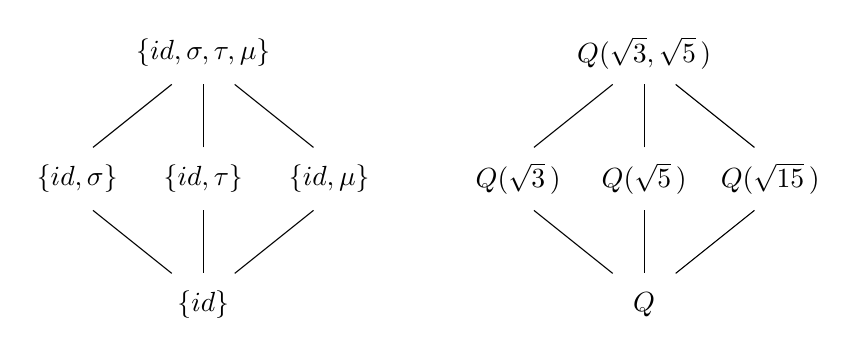
\begin{tikzpicture}[scale=0.8] %Replaced figure with tikz figure and corrected figure - TWJ 8/20/2010

\draw  (2,0.5) -- (2,1.5);
\draw  (2,-0.5) -- (2,-1.5);

\draw  (0.25,0.5) -- (1.5,1.5);
\draw  (0.25,-0.5) -- (1.5,-1.5);
\draw  (3.75,0.5) -- (2.5,1.5);
\draw  (3.75,-0.5) -- (2.5,-1.5);

\draw  (9,0.5) -- (9,1.5);
\draw  (9,-0.5) -- (9,-1.5);

\draw  (7.25,0.5) -- (8.5,1.5);
\draw  (7.25,-0.5) -- (8.5,-1.5);
\draw  (10.75,0.5) -- (9.5,1.5);
\draw  (10.75,-0.5) -- (9.5,-1.5);

\node at (0,0)  {$\{  id, \sigma \}$};
\node at (2,0)  {$\{  id, \tau \}$};
\node at (4,0)  {$\{  id, \mu \}$};
\node at (2,2)  {$\{  id, \sigma, \tau, \mu \}$};
\node at (2,-2)  {$\{  id \}$};

\node at (7,0)  {${\mathbb Q}(\sqrt{3}\, )$};
\node at (9,0)  {${\mathbb Q}(\sqrt{5}\, )$};
\node at (11,0)  {${\mathbb Q}(\sqrt{15}\, )$};
\node at (9,2)  {${\mathbb Q}(\sqrt{3}, \sqrt{5}\, )$};
\node at (9,-2)  {${\mathbb Q}$};


\end{tikzpicture}
\end{center}
\caption{$G({\mathbb Q}( \protect\sqrt{3}, \protect\sqrt{5}\, ) / {\mathbb
Q})$} 
\label{Galois1}
\end{figure}
 
 
We are now ready to state and prove the Fundamental Theorem of Galois
Theory.
 
 
\begin{theorem}
\textbf{(Fundamental Theorem of Galois Theory)}\index{Fundamental
Theorem!of Galois Theory}\label{galois:fundamental_theorem}
Let $F$ be a finite field or a field of characteristic zero. If $E$ is
a finite normal extension of $F$ with Galois group $G(E/F)$, then the
following statements are true. 
\begin{enumerate}
 
\rm \item \it
The map $K \mapsto G(E/K)$ is a bijection of subfields $K$ of $E$
containing $F$ with the subgroups of $G(E/F)$.  
 
\rm \item \it 
If $F \subset K \subset E$, then 
\[
[E:K] = |G(E/K)|
\mbox{ and }
[K:F] = [G(E/F):G(E/K)].
\]
 
\rm \item \it 
$F \subset K \subset L \subset E$ if and only if $\{ id \} \subset
G(E/L) \subset G(E/K) \subset G(E/F)$.
 
 
\rm \item \it 
$K$ is a normal extension of $F$ if and only if $G(E/K)$ is a normal 
subgroup of $G( E/F)$. In this case
\[
G(K/F) \cong G(E/F) / G( E/K ).
\]
 
\end{enumerate}
\end{theorem}
 
 
\begin{proof}
(1)
Suppose that $G(E/K) = G(E/L) = G$. Both $K$ and $L$ are fixed fields 
of $G$; hence, $K=L$ and the map defined by $K \mapsto G(E/K)$ is
one-to-one. To show that the map is onto, let $G$ be a subgroup of
$G(E/F)$ and $K$ be the field fixed by $G$. Then $F \subset K \subset
E$; consequently, $E$ is a normal extension of $K$. Thus, $G(E/K) = G$
and the map $K \mapsto G(E/K)$ is a bijection. 
 
 
(2)
By Theorem \ref{galois:extension_order_theorem}, $|G(E/K)| = [E:K]$; therefore, 
\[
|G(E/F)| = [G(E/F):G(E/K)] \cdot |G(E/K)| = [E:F] = [E:K][K:F].
\]
Thus, $[K:F] = [G(E/F):G(E/K)]$.
 
 
(3)
Statement (3) is illustrated in Figure~\ref{Galois2}.
We leave the proof of this property as an exercise.
 
\begin{figure}[htb]
\begin{center}
\tikzpreface{galois_correspondence}
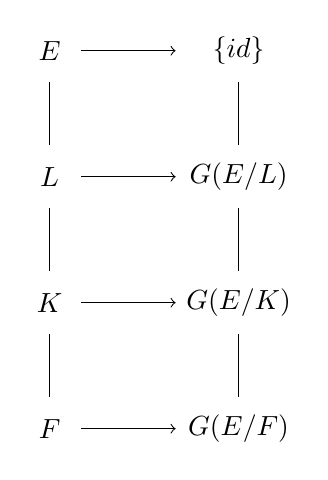
\begin{tikzpicture}[scale=0.8] %Replaced figure with tikz figure and corrected figure - TWJ 8/20/2010

\draw  (0,0.5) -- (0,1.5);
\draw  (0,2.5) -- (0,3.5);
\draw  (0,4.5) -- (0,5.5);

\draw  (3,0.5) -- (3,1.5);
\draw  (3,2.5) -- (3,3.5);
\draw  (3,4.5) -- (3,5.5);

\draw [->] (0.5,0) -- (2,0);
\draw [->] (0.5,2) -- (2,2);
\draw [->] (0.5,4) -- (2,4);
\draw [->] (0.5,6) -- (2,6);

\node at (0,0)  {$F$};
\node at (3,0)  {$G(E/F)$};

\node at (0,2)  {$K$};
\node at (3,2)  {$G(E/K)$};

\node at (0,4)  {$L$};
\node at (3,4)  {$G(E/L)$};

\node at (0,6)  {$E$};
\node at (3,6)  {$\{  id \}$};

\end{tikzpicture}
\end{center}
\caption{Subgroups of $G(E/F)$ and subfields of $E$} 
\label{Galois2}
\end{figure}
 
 
(4)
This part takes a little more work. Let $K$ be a normal extension of
$F$. If $\sigma$ is in $G(E/F)$ and $\tau$ is in $G(E/K)$, we need to
show that $\sigma^{-1} \tau \sigma$ is in $G(E/K)$; that is, we need
to show that $\sigma^{-1} \tau \sigma( \alpha) = \alpha$ for all
$\alpha \in K$.	Suppose that $f(x)$ is the minimal polynomial of
$\alpha$ over $F$. Then $\sigma( \alpha )$ is also a root of
$f(x)$ lying in $K$, since $K$ is a normal extension of $F$. Hence,
$\tau( \sigma( \alpha )) = \sigma( \alpha )$ or $\sigma^{-1} \tau 
\sigma( \alpha) = \alpha$.
 
 
Conversely, let $G(E/K)$ be a normal subgroup of $G(E/F)$. We need to
show that $F = K_{G(K/F)}$. Let $\tau \in G(E/K)$. For all $\sigma
\in G(E/F)$ there exists a $\overline{\tau} \in G(E/K)$ such that
$\tau \sigma = \sigma \overline{\tau}$.  Consequently, for all $\alpha
\in K$
\[
\tau( \sigma( \alpha ) )
= \sigma( \overline{\tau}( \alpha ) )
= \sigma( \alpha );
\]
hence, $\sigma( \alpha )$ must be in the fixed field of $G(E/K)$.
Let $\overline{\sigma}$ be the restriction of $\sigma$ to $K$. Then
$\overline{\sigma}$ is an automorphism of $K$ fixing $F$, since
$\sigma( \alpha ) \in K$ for all $\alpha \in K$; hence,
$\overline{\sigma} \in G(K/F)$. Next, we will show that the fixed
field of $G(K/F)$ is $F$. Let $\beta$ be an element in $K$ that is
fixed by all automorphisms in $G(K/F)$.  In particular,
$\overline{\sigma}(\beta) = \beta$ for all $\sigma \in G(E/F)$. 
Therefore, $\beta$ belongs to the fixed field $F$ of $G(E/F)$.
 
 
Finally, we must show that when $K$ is a normal extension of $F$, 
\[
G(K/F) \cong G(E/F) / G(E/K).
\]
For $\sigma \in G(E/F)$, let $\sigma_K$ be the automorphism of $K$
obtained by restricting $\sigma$ to $K$. Since $K$ is a normal
extension, the argument in the preceding paragraph shows that
$\sigma_K \in G( K/F)$. Consequently, we have a map \mbox{$\phi:G(E/F)
\rightarrow G(K/F)$} defined by $\sigma \mapsto \sigma_K$. This map is
a group homomorphism since
\[
\phi( \sigma \tau ) 
= (\sigma \tau)_K 
= \sigma_K \tau_K 
= \phi( \sigma) \phi( \tau ).
\]
The kernel of $\phi$ is $G(E/K)$.  By (2), 
\[
|G(E/F)| / |G(E/K)| = [K:F] = |G(K/F)|.
\]
Hence, the image of $\phi$ is $G(K/F)$ and $\phi$ is 
onto. Applying the First Isomorphism Theorem, we have
\[
G(K/F) \cong G(E/F) / G( E/K ).
\]
\end{proof}
 
 

\begin{example}{galois_x4-2}
In this example we will illustrate the Fundamental Theorem of Galois
Theory by determining the lattice of subgroups of the Galois group of
$f(x) = x^4 - 2$. We will compare this lattice to the lattice of field
extensions of ${\mathbb Q}$ that are contained in the splitting field of
$x^4-2$. The splitting field of $f(x)$ is ${\mathbb Q}( \sqrt[4]{2}, i
)$. To see this, notice that $f(x)$ factors as $(x^2 +
\sqrt{2}\, )(x^2 - \sqrt{2}\, )$; hence, the roots of $f(x)$ are $\pm
\sqrt[4]{2}$ and $\pm \sqrt[4]{2}\, i$. We first adjoin the root
$\sqrt[4]{2}$ to ${\mathbb Q}$ and then adjoin the root $i$ of $x^2 + 1$
to ${\mathbb Q}(\sqrt[4]{2}\, )$. The splitting field of $f(x)$ is then
${\mathbb Q}(\sqrt[4]{2}\, )(i) = {\mathbb Q}( \sqrt[4]{2}, i )$. 
 
 
Since $[ {\mathbb Q}( \sqrt[4]{2}\, ) : {\mathbb Q}] = 4$ and $i$ is not in
${\mathbb Q}( \sqrt[4]{2}\, )$, it must be the case that $[ {\mathbb Q}(
\sqrt[4]{2}, i ): {\mathbb Q}(\sqrt[4]{2}\, )] = 2$. Hence, $[ {\mathbb Q}(
\sqrt[4]{2}, i ):{\mathbb Q}] = 8$. The set
\[
\{ 1, \sqrt[4]{2}, (\sqrt[4]{2}\, )^2, (\sqrt[4]{2}\, )^3, i, i
\sqrt[4]{2}, i (\sqrt[4]{2}\, )^2, i(\sqrt[4]{2}\, )^3 \}
\]
is a basis of ${\mathbb Q}( \sqrt[4]{2}, i )$ over ${\mathbb Q}$. The
lattice of field extensions of ${\mathbb Q}$ contained in ${\mathbb Q}(
\sqrt[4]{2}, i)$ is illustrated in Figure~\ref{Galois3}(a).
 
%Corrected the automorphism sigma.  Suggested by R. Beezer. - TWJ 4/14/2011
The Galois group $G$ of $f(x)$ must be of order 8. Let $\sigma$ be the
automorphism defined by $\sigma( \sqrt[4]{2}\, ) = i \sqrt[4]{2}$ and
$\sigma( i ) = i$, and $\tau$ be the automorphism defined by complex
conjugation; that is, $\tau(i ) = -i$. Then $G$ has an element of
order 4 and an element of order 2. It is easy to verify by direct
computation that the elements of $G$ are $\{ id, \sigma, \sigma^2, 
\sigma^3, \tau, \sigma \tau, \sigma^2 \tau, \sigma^3 \tau \}$ and that
the relations $\tau^2 = id$, $\sigma^4 = id$, and $\tau \sigma \tau =
\sigma^{-1}$ are satisfied; hence, $G$ must be isomorphic to $D_4$.
The lattice of subgroups of $G$ is illustrated in Figure~\ref{Galois3}(b).
\end{example}
 
\begin{figure}[htb]
\begin{center}

\tikzpreface{galois_fourth_root2}
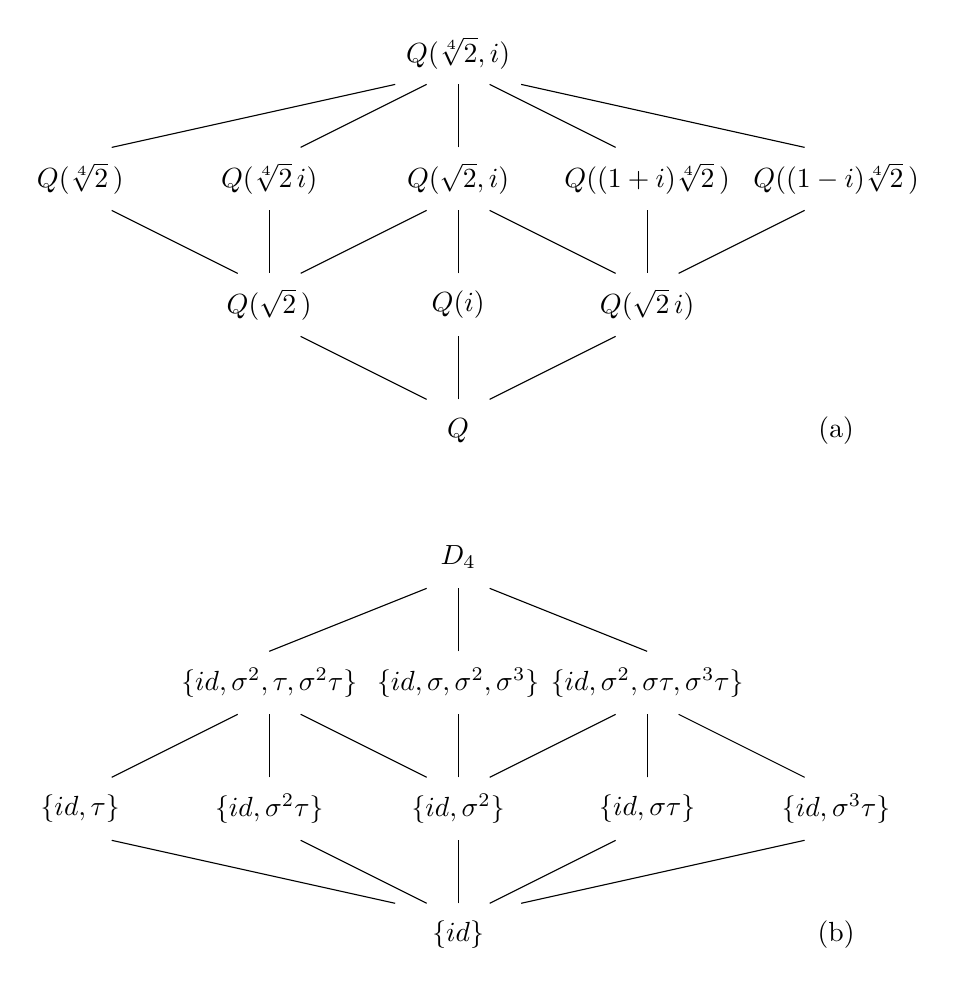
\begin{tikzpicture}[scale=0.8] %Replaced figure with tikz figure and corrected figure - TWJ 8/20/2010

\draw  (-1,0.5) -- (-5.5,1.5);
\draw  (-0.5,0.5) -- (-2.5,1.5);
\draw  (0,0.5) -- (0,1.5);
\draw  (0.5,0.5) -- (2.5,1.5);
\draw  (1,0.5) -- (5.5,1.5);


\draw  (-5.5,2.5) -- (-3.5,3.5);
\draw  (-3,2.5) -- (-3,3.5);
\draw  (-0.5,2.5) -- (-2.5,3.5);
\draw  (0,2.5) -- (0,3.5);
\draw  (5.5,2.5) -- (3.5,3.5);
\draw  (3,2.5) -- (3,3.5);
\draw  (0.5,2.5) -- (2.5,3.5);
\draw  (3,2.5) -- (3,3.5);

\draw  (-3,4.5) -- (-0.5,5.5);
\draw  (0,4.5) -- (0,5.5);
\draw  (3,4.5) -- (0.5,5.5);

\node at (0,0)  {$\{  id \}$};
\node at (-6,2)  {$\{  id, \tau \}$};
\node at (-3,2)  {$\{  id, \sigma^2 \tau \}$};
\node at (0,2)  {$\{  id, \sigma^2 \}$};
\node at (3,2)  {$\{  id, \sigma \tau \}$};
\node at (6,2)  {$\{  id, \sigma^3 \tau \}$};
\node at (-3,4)  {$\{  id, \sigma^2, \tau, \sigma^2 \tau \}$};
\node at (0,4)  {$\{  id, \sigma, \sigma^2, \sigma^3 \}$};
\node at (3,4)  {$\{  id, \sigma^2, \sigma \tau, \sigma^3 \tau \}$};
\node at (0,6)  {$D_4$};
\node at (6,0) {(b)};

\draw  (-0.5,8.5) -- (-2.5,9.5);
\draw  (0,8.5) -- (0,9.5);
\draw  (0.5,8.5) -- (2.5,9.5);

\draw  (-5.5,11.5) -- (-3.5,10.5);
\draw  (-3,11.5) -- (-3,10.5);
\draw  (-0.5,11.5) -- (-2.5,10.5);

\draw  (0,10.5) -- (0,11.5);

\draw  (5.5,11.5) -- (3.5,10.5);
\draw  (3,11.5) -- (3,10.5);
\draw  (0.5,11.5) -- (2.5,10.5);

\draw  (-5.5,12.5) -- (-1,13.5);
\draw  (-2.5,12.5) -- (-0.5,13.5);
\draw  (0,12.5) -- (0,13.5);
\draw  (2.5,12.5) -- (0.5,13.5);
\draw  (5.5,12.5) -- (1,13.5);

\node at (0,8)  {${\mathbb Q}$};
\node at (-3,10)  {${\mathbb Q}(\sqrt{2}\, )$};
\node at (0,10)  {${\mathbb Q}(i)$};
\node at (3,10)  {${\mathbb Q}(\sqrt{2}\, i)$};
\node at (-6,12)  {${\mathbb Q}( \sqrt[4]{2}\, )$};
\node at (-3,12)  {${\mathbb Q}( \sqrt[4]{2}\, i)$};
\node at (0,12)  {${\mathbb Q}( \sqrt{2}, i)$};
\node at (3,12)  {${\mathbb Q}((1 + i) \sqrt[4]{2}\,)$};
\node at (6,12)  {${\mathbb Q}( (1 - i)\sqrt[4]{2}\, )$};
\node at (0,14)  {${\mathbb Q}(\sqrt[4]{2}, i )$};
\node at (6,8) {(a)};


\end{tikzpicture}
\end{center}
\caption{Galois group of $x^4-2$}
\label{Galois3}
\end{figure}

\medskip
 
\histhead
 
 
\noindent{\small \histf
Solutions for the cubic and quartic equations were discovered in the
1500s. Attempts to find solutions for the quintic equations puzzled
some of history's best mathematicians.  In 1798, P.
Ruffini\index{Ruffini, P.} submitted a paper that claimed no such
solution could be found; however, the paper was not well received. In
1826, Niels Henrik Abel\index{Abel, Niels Henrik} (1802--1829) finally
offered the first correct proof that quintics are not always solvable
by radicals. 
 
 
Abel inspired the work of \'{E}variste Galois\index{Galois,
\'{E}variste}. Born in 1811, Galois began to display extraordinary
mathematical talent at the age of 14. He applied for entrance to
the \'{E}cole Polytechnique several times; however, he had great
difficulty meeting the formal entrance requirements, and the examiners
failed to recognize his mathematical genius. He was finally accepted
at the \'{E}cole Normale in 1829.   
 
 
Galois worked to develop a theory of solvability for polynomials.  In
1829, at the age of 17, Galois presented two papers on the
solution of algebraic equations to the Acad\'{e}mie des Sciences de
Paris.  These papers were sent to Cauchy, who subsequently lost them.
A third paper was submitted to Fourier, who died before he could read
the paper.  Another paper was presented, but was not published
until~1846.  
 
 
Galois' democratic sympathies led him into the Revolution of 1830. He
was expelled from school and sent to prison for his part in the
turmoil. After his release in 1832, he was drawn into a duel over
a love affair. Certain that he would be killed, he spent the evening
before his death outlining his work and his basic ideas for research in
a long letter to his friend Chevalier.  He  was indeed dead
the next day, at the age of 20. 
% Age of Galois' death corrected.  Suggested by K. Brooks. - TWJ 5/15/2012
\histbox
} 
 
 
 
\section{Applications}
 
 
 
\subsection*{Solvability by Radicals}

%Major clean up of the section
%TWJ 3/5/2013
 
Throughout this section we shall assume that all fields have
characteristic zero to ensure that irreducible polynomials do not have
multiple roots. The immediate goal of this section is to determine when
the roots of a polynomial $f(x)$ can be computed with a finite number of
operations on the coefficients of $f(x)$. The allowable operations are
addition, subtraction, multiplication, division, and the extraction
of $n$th roots. Certainly the solution to the quadratic equation,
$a x^2 + b x +c=0$, illustrates this process:
\[
x = \frac{-b \pm \sqrt{b^2 - 4ac}}{2a}.
\]
The only one of these operations that might demand a larger field is
the taking of $n$th roots.  We are led to the following definition.
 
 
An extension field $E$ of a field $F$ is an 
\boldemph{extension by radicals\/}\index{Extension!radical} if there exists a chain of subfields
\[
F = F_0 \subseteq F_1 \subseteq F_2 \subseteq \cdots \subseteq F_r = E
\]
such for $i = 1, 2, \ldots, r$, we have  $F_i = F_{i - 1}(\alpha_i)$ and $\alpha_i^{n_i} \in F_{i-1}$ for some positive integer $n_i$.
A polynomial $f(x)$ is \boldemph{solvable by
radicals\/}\index{Solvability by radicals} over $F$ if the splitting
field $K$ of $f(x)$ over $F$ is contained in an extension of $F$ by
radicals. Our goal is to arrive at  
criteria that will tell us whether or not a polynomial $f(x)$ is
solvable by radicals by examining the Galois group $f(x)$.
 
 
The easiest polynomial to solve by radicals is one of the form $x^n -
a$. As we discussed in Chapter~\ref{cyclic}, the roots of $x^n - 1$ are called
the \boldemph{nth roots of unity}\index{$n$th root of unity}.  These
roots are a finite subgroup of the splitting field of $x^n -1$. By
Theorem~\ref{finite:mult_group_theorem}, the $n$th roots of unity form a cyclic group.  Any
generator of this group is called a \boldemph{primitive nth root of
unity}\index{Primitive $n$th root of unity}. 


 
 

\begin{example}{galois_xn-1}
The polynomial $x^n - 1$ is solvable by radicals over ${\mathbb Q}$. The
roots of this polynomial are $1, \omega, \omega^2, \ldots,
\omega^{n-1}$, where
\[
\omega = \cos\left( \frac{2 \pi}{n} \right) + 
i \sin\left( \frac{2 \pi}{n} \right).
\]
The splitting field of $x^n - 1$ over ${\mathbb Q}$ is ${\mathbb Q}(\omega)$.
\end{example}
 
 

 
We shall prove that a polynomial is solvable by radicals if its Galois group is solvable.
Recall that a subnormal series of a group $G$ is a finite sequence
of subgroups
\[
G = H_n \supset H_{n-1} \supset \cdots \supset H_1 \supset
H_0 = \{ e \},
\]
where $H_i$ is normal in $H_{i+1}$.  A group $G$ is solvable 
if it has a subnormal series $\{ H_i \}$ such that all of the factor 
groups $H_{i+1} /H_i$ are abelian.  For example, if we examine the
series $\{ id \} \subset A_3 \subset S_3$, we see that $S_3$ is
solvable.  On the other hand, $S_5$ is not solvable, by Theorem~\ref{normal:An_simple}.
 
%Corrected the definition of a solvable group.  Suggested by K. Halasz.
%TWJ 1/10/2014 

 
\begin{lemma}\label{galois:xn-a_solvable_lemma}
Let $F$ be a field of characteristic zero and $E$ be the splitting
field of $x^n - a$ over $F$ with $a \in F$. Then $G(E/F)$ is a
solvable group.  
\end{lemma}
 
 
\begin{proof}
The roots of $x^n - a$ are $\sqrt[n]{a}, \omega	\sqrt[n]{a}, \ldots,
\omega^{n-1} \sqrt[n]{a}$, where $\omega$ is a primitive $n$th root of
unity.  Suppose that $F$ contains all of its $n$th roots of unity. 
If $\zeta$ is one of the roots of  $x^n - a$, then distinct roots of $x^n
- a$ are $\zeta, \omega \zeta, \ldots, \omega^{n-1} \zeta$, and $E =
F(\zeta)$. Since $G(E/F)$ permutes the roots $x^n - a$, the elements in 
$G(E/F)$ must be determined by their action on these roots. Let $\sigma$ 
and $\tau$ be in $G(E/F)$ and suppose that $\sigma( \zeta ) = \omega^i 
\zeta$ and $\tau( \zeta ) = \omega^j \zeta$. If $F$ contains the
roots of unity, then 
\[
\sigma \tau( \zeta ) = \sigma( \omega^j \zeta) = \omega^j \sigma(
\zeta ) = \omega^{i+j} \zeta = \omega^i \tau( \zeta ) = \tau( \omega^i
\zeta ) = \tau \sigma( \zeta ). 
\]
Therefore, $\sigma \tau = \tau \sigma$ and $G(E/F)$ is abelian, and
$G(E/F)$ must be solvable. 

%typo correction in proof.  Suggested by L.Handricks and K. Kelley.
%TWJ - 5/3/2013
 
 
 
Now suppose that $F$ does not contain a primitive $n$th root of unity.
Let $\omega$ be a generator of the cyclic group of the $n$th roots
of unity.  Let $\alpha$ be a zero of $x^n - a$. Since $\alpha$ and
$\omega \alpha$ are both in the splitting field of $x^n - a$, $\omega
= (\omega \alpha)/ \alpha$ is also in $E$. Let $K = F( \omega)$. Then
$F \subset K \subset E$. Since $K$ is the splitting field of $x^n -
1$, $K$ is a normal extension of $F$.  Therefore, any automorphism $\sigma$ in
$G(F( \omega)/ F)$ is determined by $\sigma( \omega)$.  It must be
the case that $\sigma( \omega ) = \omega^i$ for some integer $i$ since
all of the zeros of $x^n-1$ are powers of $\omega$. If $\tau( \omega
) = \omega^j$ is in $G(F(\omega)/F)$, then
\[
\sigma \tau( \omega ) = \sigma( \omega^j ) = [ \sigma(
\omega )]^j = \omega^{ij} = [\tau( \omega ) ]^i = \tau( \omega^i ) 
= \tau \sigma( \omega ). 
\]
Therefore, $G(F( \omega ) / F)$ is abelian.  By the Fundamental
Theorem of Galois Theory the series 
\[
\{ id \} \subset G(E/ F(\omega)) \subset G(E/F)
\]
is a normal series. By our previous argument, $G(E/F(\omega))$ is abelian.  Since
\[
G(E/F) /G(E/F( \omega)) \cong G(F(\omega)/F)
\]
is also abelian, $G(E/F)$ is solvable.
\end{proof}

 
 
 
\begin{lemma}\label{galois:radical_extension_lemma}
Let $F$ be a field of characteristic zero and let
\[
F = F_0 \subseteq F_1 \subseteq F_2 \subseteq \cdots \subseteq F_r = E
\]
a radical extension of $F$. Then there exists a normal radical extension 
\[
F = K_0 \subseteq K_1 \subseteq K_2 \subseteq \cdots \subseteq K_r = K
\]
such that $K$ that contains $E$ and $K_i$ is a normal extension of $K_{i-1}$.
\end{lemma}
 
 
\begin{proof}
Since $E$ is a radical extension of $F$,  there exists a chain of subfields
\[
F = F_0 \subseteq F_1 \subseteq F_2 \subseteq \cdots \subseteq F_r = E
\]
such for $i = 1, 2, \ldots, r$, we have  $F_i = F_{i - 1}(\alpha_i)$ and $\alpha_i^{n_i} \in F_{i-1}$ for some positive integer $n_i$.  We will build a normal radical extension of $F$,
\[
F = K_0 \subseteq K_1 \subseteq K_2 \subseteq \cdots \subseteq K_r = K
\]
such that $K \supseteq E$.  Define $K_1$ for be the splitting field of $x^{n_1} - \alpha_1^{n_1}$.  The roots of this polynomial are $\alpha_1, \alpha_1 \omega, \alpha_1 \omega^2, \ldots, \alpha_1 \omega^{n_1 - 1}$, where $\omega$ is a primitive  $n_1$th root of unity.  If $F$ contains all of its $n_1$ roots of unity, then  $K_1 = F(\alpha_!)$.   On the other hand, suppose that $F$ does not contain a primitive $n_1$th root of unity.  If $\beta$ is a root of  $x^{n_1} - \alpha_1^{n_1}$, then all of the roots of  $x^{n_1} - \alpha_1^{n_1}$ must be $\beta, \omega \beta, \ldots, \omega^{n_1-1}$, where  $\omega$ is a primitive  $n_1$th root of unity. In this case, $K_1 = F(\omega \beta)$.  Thus, $K_1$ is a normal radical extension of $F$ containing $F_1$.  
Continuing in this manner, we obtain
\[
F = K_0 \subseteq K_1 \subseteq K_2 \subseteq \cdots \subseteq K_r = K
\]
such that $K_i$ is a normal extension of $K_{i-1}$ and $K_i \supseteq F_i$ for $i = 1, 2, \ldots, r$.
\hspace*{0.5in}
\end{proof}


%Major rewrite of the proof.
%TWJ - 3/5/2013

%Proof should be correct now.
%TWJ - 6/5/2013



\medskip


We will now prove the main theorem about solvability by radicals.
 
 
\begin{theorem}\label{galois:solvable_by_radicals_theorem}
Let $f(x)$ be in $F[x]$, where $\chr F = 0$. If $f(x)$ is
solvable by radicals, then the Galois group of $f(x)$ over $F$ is 
solvable.
\end{theorem}
 
 
\begin{proof}
Since $f(x)$ is
solvable by radicals there exists an extension $E$ of $F$ by radicals $F = F_0 \subseteq
F_1 \subseteq \cdots \subseteq F_n = E$. By  Lemma~\ref{galois:radical_extension_lemma}, we can assume that $E$ is a splitting field $f(x)$ and   $F_i$ is normal over $F_{i-1}$.  By
the Fundamental Theorem of Galois Theory, $G(E/F_i)$ is a normal
subgroup of $G(E/F_{i-1})$.  Therefore, we have a subnormal series of
subgroups of $G(E/F)$:  
\[
\{ id \} \subset G(E/F_{n-1}) \subset \cdots \subset G(E/F_1) \subset
G(E/F).
\]
Again by the Fundamental Theorem of Galois Theory, we know that
\[
G(E/F_{i-1})/G(E/F_i) \cong G(F_i/F_{i-1}).
\]
By Lemma~\ref{galois:xn-a_solvable_lemma}, $G(F_i/F_{i-1})$ is solvable; hence, $G(E/F)$ is also
solvable. 
\mbox{\hspace{1in}}
\end{proof}


\medskip


The converse of Theorem~\ref{galois:solvable_by_radicals_theorem} is also true.  For a proof, see any of the
references at the end of this chapter.
 
 
 	   
\subsection*{Insolvability of the Quintic}
 

We are now in a position to find a fifth-degree polynomial that is not
solvable by radicals.  We merely need to find a polynomial whose
Galois group is $S_5$. We begin by proving a lemma.

%Corrected the lemma by requiring that $p$ be prime in $S_p$.  Suggested by R. Beezer and K. Brooks. - TWJ 6/15/2012

\begin{lemma}\label{galois:Sn_generating_lemma}
If $p$ is prime, then any subgroup of $S_p$ that contains a transposition and a cycle of length
$p$ must be all of $S_p$. 
\end{lemma}
 
 
\begin{proof}
Let $G$ be a subgroup of $S_p$ that contains a transposition $\sigma$
and $\tau$ a cycle of length $p$.  We may assume that $\sigma = (1 2)$.  The order of $\tau$ is $p$ and $\tau^n$ must be a cycle of length $p$ for $1 \leq n < p$.  Therefore, we may assume that $\mu = \tau^n = (1 2 i_3 \ldots i_p)$ for some $n$, where $1 \leq n < p$ (see Exercise~\ref{permute:OrderProductCycles} in Chapter~\ref{permute}).
Noting that $(1 2)(12 i_3\ldots i_p) = (2 i_3\ldots i_p)$
and $(2i_3 \ldots i_p)^k(12)(2i_3 \ldots i_p)^{-k} = (1i_k)$, we can obtain all
the transpositions of the form $(1n)$ for $1 \leq n < p$. However, these
transpositions generate all transpositions in $S_p$, since $(1j)(1 i)(1
j) = (i j)$.  The transpositions generate $S_p$. 
\end{proof}
 
 
\medskip
\begin{figure}
\begin{center}
\tikzpreface{galois_quintic}
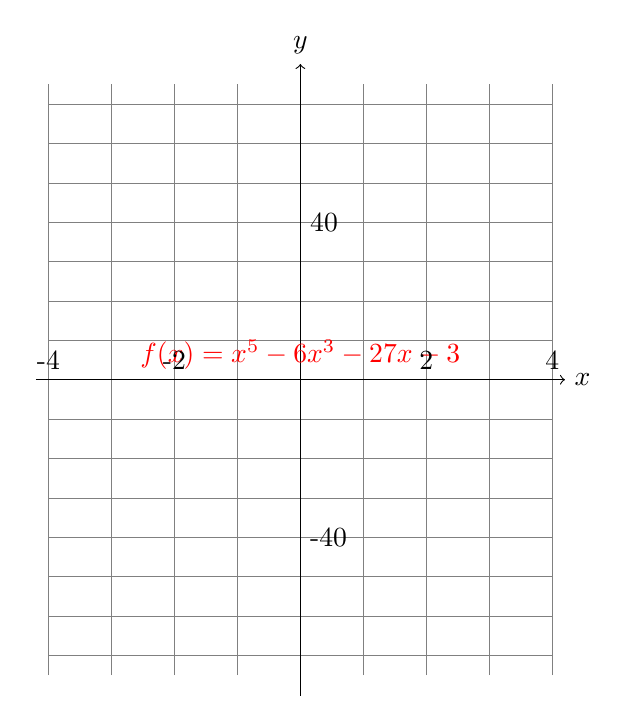
\begin{tikzpicture}[xscale=0.8,yscale=0.05,domain=-3.2:3.2,samples=320]
\draw[very thin,color=gray] (-4,-75) grid [xstep=1,ystep=10] (4,75);

\draw[->] (-4.2,0) -- (4.2,0) node[right] {$x$}; 
\draw[->] (0,-80.2) -- (0,80.2) node[above] {$y$};

\draw[thick,color=red]	plot[smooth,id=quintic]	function{x**5 - 6 *x**3 - 27 *x - 3}	node[above] {$f(x) =x^5 - 6 x^3 - 27 x - 3$};

\node [right] at (0,40)  {40};
\node [right] at (0,-40)  {-40};

\node [above] at (4,0)  {4};
\node [above] at (2,0)  {2};
\node [above] at (-2,0)  {-2};
\node [above] at (-4,0)  {-4};

\end{tikzpicture}


\end{center}
\caption{The graph of $f(x) = x^5 - 6 x^3 - 27 x - 3$}
\label{Galois4}
\end{figure}

 

\begin{example}{galois_x5}
We will show that $f(x) = x^5 - 6 x^3 - 27 x - 3 \in {\mathbb Q}[x]$ is
not solvable. We claim that the Galois group of $f(x)$ over ${\mathbb Q}$
is $S_5$. By Eisenstein's Criterion, $f(x)$ is irreducible and,
therefore, must be separable. The derivative of $f(x)$ is $f'(x) = 5
x^4 - 18 x^2 - 27$; hence, setting $f'(x) = 0$ and solving, we find
that the only real roots of $f'(x)$ are
\[
x = \pm \sqrt{ \frac{6 \sqrt{6} + 9 }{5} }.
\]
Therefore, $f(x)$ can have at most one maximum and one minimum.  It is
easy to show that $f(x)$ changes sign between $-3$ and $-2$, between
$-2$ and $0$, and once again between $0$ and $4$
(Figure~\ref{Galois4}). Therefore, $f(x)$ has exactly three distinct
real roots. The remaining two roots of $f(x)$ must be complex
conjugates. Let $K$ be the splitting field of $f(x)$. Since $f(x)$ has
five distinct roots in $K$ and every automorphism of $K$ fixing ${\mathbb
Q}$ is determined by the way it permutes the roots of $f(x)$, we know
that $G(K/{\mathbb Q})$ is a subgroup of $S_5$. Since $f$ is irreducible,
there is an element in $\sigma \in G(K/{\mathbb Q})$ such that $\sigma(a)
= b$ for two roots $a$ and $b$ of $f(x)$. The automorphism of ${\mathbb
C}$ that takes $a+bi \mapsto a-bi$ leaves the real roots fixed and
interchanges the complex roots; consequently, $G(K/{\mathbb Q} ) \subset
S_5$. By Lemma~\ref{galois:Sn_generating_lemma}, $S_5$ is generated by a transposition and an
element of order 5; therefore, $G(K/{\mathbb Q} )$ must be all of $S_5$. By
Theorem~\ref{normal:An_simple}, $S_5$ is not solvable. Consequently, $f(x)$ cannot be
solved by radicals.  
% Changed $G(K/F )$ to $G(K/{\mathbb Q} )$.  Suggested by Aleks Vlasev. - TWJ 8/10/2011
\end{example}
 
 
 
\subsection*{The Fundamental Theorem of Algebra}
 
 
It seems fitting that the last theorem that we will state and prove
is the Fundamental Theorem of Algebra. This theorem was first proven
by Gauss in his doctoral thesis.  Prior to Gauss's proof, mathematicians 
suspected that there might exist polynomials over the real and complex 
numbers having no solutions. The Fundamental Theorem of Algebra states
that every polynomial over the complex numbers factors into distinct
linear factors. 
 
 
\begin{theorem}[Fundamental Theorem of Algebra]\index{Fundamental Theorem!of Algebra}
The field of complex numbers is algebraically closed; that is, every
polynomial in ${\mathbb C}[x]$ has a root in ${\mathbb C}$. 
\end{theorem}
 
 
For our proof we shall assume two facts from calculus.  We need the
results that every polynomial of odd degree over ${\mathbb R}$ has a real
root and that every positive real number has a square root.  
 
 
\medskip
 
 
\begin{proof}
Suppose that $E$ is a proper finite field extension of the complex 
numbers. Since any finite extension of a field of characteristic zero
is a simple extension, there exists an $\alpha \in E$ such that $E =
{\mathbb C}( \alpha )$ with $\alpha$ the root of an irreducible
polynomial $f(x)$ in ${\mathbb C}[x]$. The splitting field $L$ of $f(x)$ 
is a finite normal separable extension of ${\mathbb C}$ that contains  $E$.
We must show that it is impossible for $L$ to be a proper extension of
${\mathbb C}$. 
 
 
Suppose that $L$ is a proper extension of ${\mathbb C}$. Since $L$ is the
splitting field of $f(x)(x^2 + 1)$ over ${\mathbb R}$, $L$ is a finite
normal separable extension of ${\mathbb R}$. Let $K$ be the fixed field
of a Sylow 2-subgroup $G$ of $G(L/{\mathbb R})$. Then $L \supset  K
\supset {\mathbb R}$ and $|G( L / K )| =[L:K]$. Since $[L : {\mathbb R}] =
[L:K][K:{\mathbb R}]$, we know that $[K:{\mathbb R}]$ must be odd.
Consequently, $K = {\mathbb R}(\beta)$ with $\beta$ having a minimal
polynomial $f(x)$ of odd degree.  Therefore, $K = {\mathbb R}$. 
 
 
We now know that $G(L/{\mathbb R})$ must be a 2-group. It follows that
$G(L / {\mathbb C})$ is a 2-group.  We have assumed that $L \neq {\mathbb
C}$; therefore, $|G(L / {\mathbb C})| \geq 2$.  By the first Sylow
Theorem and the Fundamental Theorem of Galois Theory, there exists a
subgroup $G$ of $G(L/{\mathbb C})$ of index 2 and a field $E$ fixed
elementwise by $G$. Then $[E:{\mathbb C}] = 2$ and there exists an
element $\gamma \in E$ with minimal polynomial $x^2 + b x + c$ in
${\mathbb C}[x]$.  This polynomial has roots $( - b \pm \sqrt{b^2 - 4
c}\, ) / 2$ that are in ${\mathbb C}$, since $b^2 - 4 c$ is in ${\mathbb
C}$.  This is impossible; hence, $L = {\mathbb C}$.
\end{proof}
 
 
\medskip
 
 
Although our proof was strictly algebraic, we were forced to rely on
results from calculus.  It is necessary to assume the completeness
axiom from analysis to show that every polynomial of odd degree has a
real root and that every positive real number has a square root.  It
seems that there is no possible way to avoid this difficulty and
formulate a purely algebraic argument.  It is somewhat amazing that
there are several elegant proofs of the Fundamental Theorem of Algebra
that use complex analysis.  It is also interesting to note that we can
obtain a proof of such an important theorem from two very different
fields of mathematics. 
 
 
 
\markright{EXERCISES}
\section*{Exercises}
\exrule
 
 
{\small
\begin{enumerate}
 
 
\item
Compute each of the following Galois groups. Which of these field
extensions are normal field extensions? If the extension is not
normal, find a normal extension of ${\mathbb Q}$ in which the extension
field is contained.
\begin{multicols}{2}
\begin{enumerate}

\item 
$G({\mathbb Q}(\sqrt{30}\, ) / {\mathbb Q})$

\item 
$G({\mathbb Q}(\sqrt[4]{5}\, ) / {\mathbb Q})$

\item 
$G( {\mathbb Q}(\sqrt{2}, \sqrt{3}, \sqrt{5}\, )/ {\mathbb Q} )$

\item 
$G({\mathbb Q}(\sqrt{2}, \sqrt[3]{2}, i) / {\mathbb Q})$

\item 
$G({\mathbb Q}(\sqrt{6}, i) / {\mathbb Q})$


\end{enumerate}

\end{multicols}
 

 
 
\item
Determine the separability of each of the following polynomials.
\begin{multicols}{2}
\begin{enumerate}

\item 
$x^3 + 2 x^2 - x - 2$ over ${\mathbb Q}$

\item 
$x^4 + 2 x^2 + 1$ over ${\mathbb Q}$

\item 
$x^4 + x^2 + 1$ over ${\mathbb Z}_3$

\item 
$x^3 +x^2 + 1$ over ${\mathbb Z}_2$

\end{enumerate}
\end{multicols}
 

\item
Give the order and describe a generator of the Galois group of
$\gf(729)$ over~$\gf(9)$.

 
\item
Determine the Galois groups of each of the following polynomials in
${\mathbb Q}[x]$; hence, determine the solvability by radicals of each 
of the polynomials.
\begin{multicols}{2}
\begin{enumerate}

\item 
$x^5 - 12 x^2 + 2$

\item 
$x^5 - 4 x^4 + 2 x + 2$

\item 
$x^3 - 5$

\item 
$x^4 - x^2 - 6$

\item 
$x^5 + 1$

\item 
$(x^2 - 2)(x^2 + 2)$

\item 
$x^8 - 1$

\item 
$x^8 + 1$

\item 
$x^4 - 3 x^2 -10$


\end{enumerate}
\end{multicols}
 
 
 
\item
Find a primitive element in the splitting field of each of the
following polynomials in ${\mathbb Q}[x]$.
\begin{multicols}{2}
\begin{enumerate}

\item 
$x^4 - 1$

\item 
$x^4 - 8 x^2 + 15$

\item 
$x^4 - 2 x^2 - 15$

\item 
$x^3 - 2$

\end{enumerate}
\end{multicols}
  
 
%******************************THEORY*****************
 
 
 
 
\item
Prove that the Galois group of an irreducible quadratic polynomial is
isomorphic to ${\mathbb Z}_2$.
 
 
\item
Prove that the Galois group of an irreducible cubic polynomial is
isomorphic to $S_3$ or ${\mathbb Z}_3$.
 
 
\item
Let $F \subset K \subset E$ be fields. If E is a normal extension of
$F$, show that $E$ must also be a normal extension of $K$.
 
 
\item
Let $G$ be the Galois group of a polynomial of degree $n$.  Prove
that $|G|$ divides~$n!$.
 
 
\item
Let $F \subset E$.  If $f(x)$ is solvable over $F$, show that $f(x)$
is also solvable over $E$.
 
 
\item
Construct a polynomial $f(x)$ in ${\mathbb Q}[x]$ of degree 7 that is not
solvable by \linebreak radicals.
 
 
\item
Let $p$ be prime.  Prove that there exists a polynomial $f(x) \in
{\mathbb Q}[x]$ of degree $p$ with Galois group isomorphic to $S_p$.
Conclude that for each prime $p$ with $p \geq 5$ there exists a
polynomial of degree $p$ that is not solvable by radicals. 
 
 
\item
Let $p$ be a prime and ${\mathbb Z}_p(t)$ be the field of rational
functions over ${\mathbb Z}_p$.  Prove that $f(x) = x^p - t$ is an
irreducible polynomial in ${\mathbb Z}_p(t)[x]$.  Show that $f(x)$ is not
separable. 
 
 
\item
Let $E$ be an extension field of $F$. Suppose that $K$ and $L$ are two 
intermediate fields.  If there exists an element $\sigma \in G(E/F)$
such that $\sigma(K) = L$, then $K$ and $L$ are said to be \boldemph{
conjugate fields}\index{Conjugate fields}\index{Field!conjugate}.
Prove that $K$ and $L$ are conjugate if and only if $G(E/K)$ and
$G(E/L)$ are conjugate subgroups of $G(E/F)$. 
 
 
\item 
Let $\sigma \in \aut( {\mathbb R} )$.  If $a$ is a positive real
number, show that $\sigma( a) > 0$.
 
 
\item 
Let $K$ be the splitting field of $x^3 + x^2 + 1 \in {\mathbb Z}_2[x]$.
Prove or disprove that $K$ is an extension by radicals.
 
\item
Let $F$ be a field such that ${\rm char}\, F \neq 2$. Prove that the
splitting field of $f(x) = a x^2 + b x + c$ is $F( \sqrt{\alpha}\, )$,
where $\alpha = b^2 - 4ac$. 
 
 
\item
Prove or disprove: Two different subgroups of a Galois group will
have different fixed fields.
 
 
 
\item
Let $K$ be the splitting field of a polynomial over $F$. If $E$ is a
field extension of $F$ contained in $K$ and $[E:F] = 2$, then $E$ is
the splitting field of some polynomial in $F[x]$.
 
  
 
\item
We know that the cyclotomic polynomial
\[
\Phi_p(x) = \frac{x^p - 1}{x-1} = x^{p-1} + x^{p-2} + \cdots
+ x + 1
\]
is irreducible over ${\mathbb Q}$ for every prime $p$. Let $\omega$ be a
zero of $\Phi_p(x)$, and consider the field ${\mathbb Q}(\omega)$.
\begin{enumerate}
 
 \item
Show that $\omega, \omega^2, \ldots, \omega^{p-1}$ are distinct zeros of
$\Phi_p(x)$, and conclude that they are all the zeros of $\Phi_p(x)$.
 
 \item
Show that $G( {\mathbb Q}( \omega ) / {\mathbb Q} )$ is abelian of order
$p-1$. 
 
 \item
Show that the fixed field of $G( {\mathbb Q}( \omega ) / {\mathbb Q} )$ is
${\mathbb Q}$. 
 
\end{enumerate}
 
  
\item
Let $F$ be a finite field or a field of characteristic zero.
Let $E$ be a finite normal extension of $F$ with Galois group
$G(E/F)$. Prove that $F \subset K \subset L \subset E$ if and 
only if $\{ id \} \subset G(E/L) \subset G(E/K) \subset G(E/F)$.
 
 
\item
Let $F$ be a field of characteristic zero and let $f(x) \in F[x]$ be
a separable polynomial of degree $n$. If $E$ is the splitting field
of $f(x)$, let $\alpha_1, \ldots, \alpha_n$ be the roots of $f(x)$ in
$E$. Let $\Delta = \prod_{i < j} (\alpha_i - \alpha_j)$.  We
define the \boldemph{discriminant\/}\index{Discriminant!of a separable
polynomial}\label{discriminant} of $f(x)$ to be $\Delta^2$. 
\begin{enumerate}
 
 \item
If $f(x) = x^2 + b x + c$, show that $\Delta^2 = b^2 - 4c$.
 
 \item
If $f(x) = x^3 + p x + q$, show that $\Delta^2 = - 4p^3 - 27q^2$.
 
 \item
Prove that $\Delta^2$ is in $F$.
 
 \item
If $\sigma \in G(E/F)$ is a transposition of two roots of $f(x)$, show
that $\sigma( \Delta )~=~-\Delta$.
 
  \item
If $\sigma \in G(E/F)$ is an even permutation of the roots of $f(x)$, show
that $\sigma( \Delta ) = \Delta$.
 
  \item
Prove that $G(E/F)$ is isomorphic to a subgroup of $A_n$ if and
only if $\Delta \in F$.
 
 \item
Determine the Galois groups of $x^3 + 2 x - 4$ and $x^3 + x -3$.
 
\end{enumerate}

%Exercise corrected and revised.
%TWJ 30/4/2013
 
 
\end{enumerate}
}
 
 
 
 
\subsection*{References and Suggested Readings}
 
{\small
\begin{itemize}
 
\item[\textbf{[1]}] %Reference updated - 21 August 2010 - TWJ
Artin, E. \textit{Theory: Lectures Delivered at the University of Notre Dame (Notre Dame Mathematical Lectures, Number 2)}. 
Dover, Mineola, NY, 1997.
 
\item[\textbf{[2]}]
Edwards, H. M. \textit{Galois Theory}. Springer-Verlag, New
York, 1984.
 
\item[\textbf{[3]}] %Reference updated - 21 August 2010 - TWJ
Fraleigh, J. B. 
\textit{A First Course in Abstract Algebra}. 7th ed.
Pearson, Upper Saddle River, NJ, 2003. 
 
\item[\textbf{[4]}] %Reference updated - 21 August 2010 - TWJ
Gaal, L. \textit{Classical Galois Theory with Examples}. 
American Mathematical Society, Providence, 1979. 
 
\item[\textbf{[5]}]
Garling, D. J. H. \textit{A Course in Galois Theory}.
Cambridge University Press, Cambridge, 1986.
 
 
\item[\textbf{[6]}] %Out of print  - 19 August 2010 - TWJ
Kaplansky, I. \textit{Fields and Rings}. 2nd ed. University of Chicago
Press, Chicago, 1972. 
 
\item[\textbf{[7]}]
Rothman, T. ``The Short Life of \'{E}variste Galois,'' {\it
Scientific American}, April 1982, 136--49.
 
\end{itemize}
}
 
\sagesection
 
   %Galois Theory
%
% RAB, 2009/01/28
% Include GFDL as an appendix
%
% To build index with included sectioning info via "style file" execute:
%    makeindex -s aata-index-style.ist aata.idx
% See:  http://www.troubleshooters.com/linux/lyx/makeindex.htm
% Needs "\phantomsection", http://www.tug.org/applications/hyperref/manual.html
%
\backmatter
%%%%(c)
%%%%(c)  This file is a portion of the source for the textbook
%%%%(c)
%%%%(c)    Abstract Algebra: Theory and Applications
%%%%(c)    Copyright 1997 by Thomas W. Judson
%%%%(c)
%%%%(c)  See the file COPYING.txt for copying conditions
%%%%(c)
%%%%(c)
\chapter*{Hints and Solutions}
 
 
\addcontentsline{toc}{chapter}{Hints and Solutions}
\pagestyle{myheadings}
\markboth{HINTS AND SOLUTIONS}{HINTS AND SOLUTIONS}
 
 
 
\subsection*{Chapter 1. Preliminaries}
 
 
{\small
\begin{itemize}
 
\item[1.]
(a) $\{ 2 \}$.
(b) $\{ 5 \}$.
 
\item[2.]
(a) $\{ (a,1), (a,2), (a,3), (b,1), (b,2), (b,3), (c,1), (c,2),
(c,3) \}$. \\
(d) $\emptyset$.
 
\item[6.]
If $x \in A \cup (B \cap C)$, then either $x \in A$ or $x \in B \cap 
C$  $\Rightarrow x \in A \cup B \text{ and } A \cup C \Rightarrow x
\in (A \cup B) \cap (A \cup C) \Rightarrow  A \cup (B \cap C) \subset 
(A \cup B) \cap (A \cup C)$. 
 
Conversely, $x \in (A \cup B) \cap (A \cup C) \Rightarrow  x \in A 
\cup B \text{ and } A \cup C \Rightarrow x \in A  \text{ or } x \text{ is in
both } $B$ \text{ and } $C$  \Rightarrow x \in A \cup (B \cap C) \Rightarrow
(A \cup B) \cap (A \cup C) \subset A \cup (B \cap C)$. Hence, $A \cup 
(B \cap C) = (A \cup B) \cap (A \cup C)$. 
 
\item[10.]
$(A \cap B) \cup (A \setminus B) \cup (B \setminus A) = (A \cap B) \cup 
(A \cap B') \cup (B \cap A') = [A \cap (B \cup B')] \cup (B \cap A')
= A \cup (B \cap A') = (A \cup B) \cap (A \cup A') = A \cup B$.
 
 
\item[14.]
$A \setminus (B \cup C) = A \cap (B \cup C)'
= (A \cap A) \cap (B' \cap C')
= (A \cap B') \cap (A \cap C') = 
(A \setminus B) \cap (A \setminus C)$. 
 
\item[17.]
(a) Not a map. $f(2/3)$ is undefined. \\
(c) Not a map. $f(1/2) =3/4$ and $f(2/4)=3/8$.
 
\item[18.]
(a)  One-to-one but not onto. $f({\mathbb R} ) = \{ x \in {\mathbb R} : x
> 0 \}$. \\
(c) Neither one-to-one nor onto.
 
\item[20.]
(a) $f(n) = n + 1$.
 
\item[22.]
(a) Let $x, y \in A$. Then $g(f(x)) = (g \circ f)(x) = (g \circ
f)(y) = g(f(y)) \Rightarrow f(x) = f(y) \Rightarrow x = y$,  so $g
\circ f$ is one-to-one. \\
(b) Let $c \in C$, then $c = (g \circ f)(x) = g(f(x))$ for some
$x \in A$. Since $f(x) \in B$, $g$ is onto.
 
\item[23.]
$f^{-1}(x) = (x+1)/(x-1)$.
 
\item[24.]
(a)  Let $y \in f(A_1 \cup A_2) \Rightarrow$ there exists an $x
\in A_1 \cup A_2$ such that $f(x) = y \Rightarrow y \in f(A_1)$ or
$f(A_2) \Rightarrow y \in f(A_1) \cup f(A_2) \Rightarrow f(A_1 \cup A_2)
\subset f(A_1) \cup f(A_2)$.
 
Conversely, let $y \in f(A_1) \cup f(A_2) \Rightarrow y \in f(A_1)$ or
$f(A_2) \Rightarrow$ there exists an $x \in A_1$ or there exists an
$x \in A_2$ such that $f(x) = y \Rightarrow$ there exists an $x \in
A_1 \cup A_2$ such that $f(x) = y \Rightarrow f(A_1) \cup f(A_2)
\subset f(A_1 \cup A_2)$. Hence, $f(A_1 \cup A_2) = f(A_1) \cup f(A_2)$. 
 
\item[25.]
(a) Not an equivalence relation. Fails to be symmetric.\\
(b) Not an equivalence relation. Fails to be reflexive since 0 is not equivalent to itself.\\
(c) Not an equivalence relation. Fails to be transitive.

%Solution to (b) corrected.  Suggested by R. Nilange.
%TWJ 8/14/2013 


 
\item[28.]
Let $X = {\mathbb N} \cup \{ \sqrt{2}\, \}$ and define $x \sim y$ if $x + y
\in {\mathbb N}$.
 
\end{itemize}
}
 
 
 
\subsection*{Chapter 2. The Integers}
 
 
{\small
\begin{itemize}
 
 
\item[1.]
$S(1): [1(1+1)(2(1) + 1)]/6 = 1 = 1^2$ is true. Assume $S(k): 1^2 +2^2
+ \cdots + k^2 = [k(k+1)(2k+1)]/6$ is true. Then $1^2 + 2^2 + \cdots +
k^2 + (k+1)^2 = [k(k+1)(2k+1)]/6 + (k+1)^2 = [(k+1)((k+1) +1)(2(k+1) +
1)]/6$, so $S(k+1)$ is true. Thus $S(n)$ is true for all positive
integers $n$. 
 
\item[3.]
$S(4): 4! = 24 > 16 =2^4$ is true. Assume $S(k): k! >2^k$ is true.
Then $(k+1)! = k! (k+1) > 2^k \cdot 2 = 2^{k+1}$, so $S(k+1)$ is true.
Thus $S(n)$ is true for all positive integers $n$. 
 
 
\item[8.]
Look at the proof in Example~\ref{example:integers:binomial_theorem}.
 
\item[11.]
$S(0): (1+x)^0 -1 = 0 \geq 0 = 0 \cdot x$ is true. Assume $S(k):
(1+x)^k -1 \geq kx$ is true. Then $(1+x)^{k+1} - 1 = (1+x)(1+x)^k -1 =
(1+x)^k + x(1+x)^k -1 \geq kx + x(1+x)^k \geq kx + x = (k+1)x$, so
$S(k+1)$ is true. Thus $S(n)$ is true for all positive integers $n$.
 
 
\item[15.]
(a) $(14)14 + (-5)39 = 1$.\\
(c) $(3709) 1739 + (-650) 9923 = 1$.\\
(e) $(881) 23771 + (-1050) 19945 = 1$.
 
 
\item[17.]
(b) Use mathematical induction.
(c) Show that $f_1 = 1$, $f_2 = 1$, and $f_{n + 2}
= f_{n + 1} + f_n$.
(d) Use part (c).
(e) Use part (b) and Problem 16.
 
 
\item[19.]
Use the Fundamental Theorem of Arithmetic.
 
 
\item[23.]
Let $S = \{s \in {\mathbb N} : a \mid s$, $b \mid s \}$. $S \neq \emptyset$,
since $|ab| \in S$. By the Principle of Well-Ordering, $S$ contains a
least element $m$. To show uniqueness, suppose that $a \mid n$ and $b
\mid n$ for some $n \in {\mathbb N}$. By the division algorithm, there
exist unique integers $q$ and $r$ such that $n = mq + r$, where $0
\leq r < m$. $a \mid m$, $b \mid m$, $a \mid n$, $b \mid n \Rightarrow a
\mid r$, $b \mid r \Rightarrow r = 0$ by the minimality of $m$.
Therefore, $m \mid n$. 
 
 
\item[27.]
Since $\gcd(a,b)=1$, there exist integers $r$ and $s$ such that $ar +
bs =1 \Rightarrow acr+bcs =c$. Since $a \mid a$ and $a \mid bc$, $a
\mid c$.
 
 
\item[29.]
Every prime number greater than 3, must be of the form $6 n \pm 1$ for some $n \in \mathbb N$.
Suppose that there are only a finite number of primes of  the form $6n +1$,
\[
p_1 = 6n_1 + 1, p_2 = 6 n_2 + 1, \ldots, p_k = 6n_k + 1.
\]
Let $p = p_1 p_2 \cdots p_k + 1$.  Then $p$ must be of the form $6m + 1$ for some $m \in \mathbb N$.  Since $p$ is not divisible by any prime of the form $6 n -1$ or $p_1, p_2, \ldots, p_k$, it must be prime which contradicts the fact that the only primes of the form $6n + 1$ are $p_1, p_2, \ldots, p_k$.

%Replaced the incorrect hint with a correct solution.
%D. Keeler pointed out the error.  TWJ 1/10/2014
 
\end{itemize}
}
 
 
 
\subsection*{Chapter 3. Groups}
 
 
{\small
\begin{itemize}
 
\item[1.]
(a) $\{ \ldots, -4, 3, 10, \ldots \}$.
(c) $\{ \ldots, -8, 18, 44, \ldots \}$.
(e) $\{ \ldots, -1, 5, 11, \ldots \}$.
 
\item[2.]
(a) Not a group.
(c) A group.
 
 
 
\item[6.] 
\raisebox{-24pt}{\parbox{1.85in}{
\begin{tabular}{c|cccc}
$\cdot$ & 1  & 5  & 7  & 11 \\
\hline
1     & 1  & 5  & 7  & 11 \\
5     & 5  & 1  & 11 & 7 \\
7     & 7  & 11 & 1  & 5 \\
11    & 11 & 7  & 5  & 1
\end{tabular}
}}
 
 
\item[8.]
Pick two matrices. Almost any pair will work.
 
\item[15.]
There is a group of order 6 that is nonabelian.
 
\item[16.]
Look at the symmetry group of an equilateral triangle or a square.
 
\item[17.]
There are actually five different groups of order 8.
 
\item[18.]
Let
\[
\sigma
=
\begin{pmatrix}
1   & 2   & \cdots & n \\
a_1 & a_2 & \cdots & a_n
\end{pmatrix}
\]
be in $S_n$. All of the $a_i$'s must be distinct.  There are $n$ ways
to choose $a_1$, $n-1$ ways to choose $a_2$, $\ldots$, 2 ways to
choose $a_{n-1}$, and only one way to choose $a_n$. Therefore, we can form
$\sigma$ in $n(n-1) \cdots 2 \cdot 1 = n!$ ways.
 
\item[25.]
$(aba^{-1})^n = (aba^{-1})(aba^{-1}) \cdots (aba^{-1}) 
= ab(aa^{-1})b(aa^{-1})b \cdots (aa^{-1})ba^{-1} = ab^na^{-1}$.
 
\item[31.]
$abab = (ab)^2 = e = a^2 b^2 = aabb\Rightarrow  ba = ab$.
 
\item[35.]
$H_1 = \{ id \}$, $H_2 = \{ id, \rho_1, \rho_2  \}$, $H_3 = \{ id,
\mu_1 \}$, $H_4 = \{ id, \mu_2 \}$, $H_5 = \{ id, \mu_3 \}$, $S_3$.
 
\item[41.]
$id = 1 = 1 + 0 \sqrt{2}$, $(a + b \sqrt{2}\, )(c + d \sqrt{2}\, ) = 
(ac + 2bd) + (ad + bc)\sqrt{2}$, and $(a + b \sqrt{2}\, )^{-1} = a/(a^2
-2b^2) - b\sqrt{2}/(a^2 - 2 b^2)$.
 
\item[46.]
Not a subgroup. Look at $S_3$.
 
\item[49.]
$a^4b =ba \Rightarrow b = a^6 b = a^2 b a \Rightarrow ab = a^3 b a =
ba$. 
 
\end{itemize}
}
 
\subsection*{Chapter 4. Cyclic Groups}
 
{\small
\begin{itemize}
 
\item[1.]
(a) False.
(c) False.
(e) True.
 
\item[2.]
(a) 12.
(c) Infinite.
(e) 10.
 
\item[3.]
(a) $7 {\mathbb Z} = \{ \ldots, -7, 0, 7, 14, \ldots \}$. 
(b) $\{ 0, 3, 6, 9, 12, 15, 18, 21 \}$. \\
(c) $\{ 0 \}, \{ 0, 6 \}, \{ 0, 4, 8 \}, \{ 0, 3, 6, 9 \}, \{ 0,
2, 4, 6, 8, 10 \}$. \\
(g) $\{ 1, 3, 7, 9 \}$.
(j) $\{ 1, -1, i, -i \}$.
 
\item[4.]
(a) 
\raisebox{-6.5pt}{\parbox{4in}{
\[
\begin{pmatrix}
1 & 0 \\
0 & 1
\end{pmatrix},
\begin{pmatrix}
-1 & 0 \\
0 & -1
\end{pmatrix},
\begin{pmatrix}
0 & -1 \\
1 & 0
\end{pmatrix},
\begin{pmatrix}
0 & 1 \\
-1 & 0
\end{pmatrix}.
\]
}}

(c) 
\raisebox{-23.5pt}{\parbox{4in}{
\[
\begin{array}{c}
\begin{pmatrix}
1 & 0 \\
0 & 1
\end{pmatrix},
\begin{pmatrix}
1 & -1 \\
1 & 0
\end{pmatrix},
\begin{pmatrix}
-1 & 1 \\
-1 & 0
\end{pmatrix},\\ \\
\begin{pmatrix}
0 & 1 \\
-1 & 1
\end{pmatrix},
\begin{pmatrix}
0 & -1 \\
1 & -1
\end{pmatrix},
\begin{pmatrix}
-1 & 0 \\
0 & -1
\end{pmatrix}.
\end{array}
\]
}}
 
\item[10.]
(a) $0, 1, -1$.
(b) $1, -1$.
 
\item[11.]
1, 2, 3, 4, 6, 8, 12, 24.
 
\item[15.]
(a) $3i -3$.
(c) $43 -18i$.
(e) $i$.
 
\item[16.]
(a) $\sqrt{3} + i$.
(c) $-3$.
 
\item[17.]
(a) $\sqrt{2} \mbox{ cis}( 7 \pi /4)$.
(c) $2 \sqrt{2} \mbox{ cis}( \pi /4)$.
(e) $3 \mbox{ cis}(3 \pi/2)$.
 
\item[18.]
(a) $(1-i)/2$.
(c) $16(i -\sqrt{3}\, )$.
(e) $-1/4$.
 
\item[22.]
(a) 292.
(c) 1523.
 
 
\item[27.]
$|\langle g \rangle \cap \langle h \rangle| = 1$.
 
 
\item[31.]
The identity element in any group has finite order. Let $g, h \in G$
have orders $m$ and $n$, respectively. Since $(g^{-1})^m = e$ and
$(gh)^{mn} = e$, the elements of finite order in $G$ form a subgroup
of $G$.
 
\item[37.]
If $g$ is an element distinct from the identity in $G$, $g$ must
generate $G$; otherwise, $\langle g \rangle$ is a nontrivial proper
subgroup of $G$.
 
\end{itemize}
}
 
\subsection*{Chapter 5. Permutation Groups}
 
{\small
\begin{itemize}
 
 
\item[1.]
(a) $(12453)$.
(c) $(13)(25)$.
 
 
\item[2.]
(a) $(135)(24)$.
(c) $(14)(23)$.
(e) $(1324)$.
(g) $(134)(25)$.
(n) $(17352)$. 
 
 
\item[3.]
(a) $(16)(15)(13)(14)$.
(c) $(16)(14)(12)$.
 
\item[4.]
$(a_1, a_{n}, a_{n-1}, \ldots, a_2)$.
  
 
\item[5.]
(a) $\{ (13), (13)(24), (132), (134), (1324), (1342) \}$. 
Not a subgroup.
 
 
\item[8.]
$(12345)(678)$.
 
 
\item[11.]
Permutations of the form $(1)$, $(a_1, a_2)(a_3, a_4)$, 
$(a_1, a_2, a_3)$, $(a_1, a_2, a_3, a_4, a_5)$ are possible for $A_5$.
 
\item[17.]
$(123)(12) = (13) \neq (23) = (12)(123)$.
 
 
\item[25.]
Use the fact that $(ab)(bc) = (abc)$ and $(ab)(cd) = (abc)(bcd)$.
 
 
\item[30.]
(a) 
Show that $\sigma \tau \sigma^{-1 }(i) = ( \sigma(a_1), 
\sigma(a_2), \ldots, \sigma(a_k))(i)$ for $1 \leq i \leq n$.
 
 
\end{itemize}
}
 
\subsection*{Chapter 6. Cosets and Lagrange's Theorem}
 
{\small
\begin{itemize}
 
\item[1.]
The order of $g$ and the order $h$ must both divide the order of $G$.
The smallest number that 5 and 7 both divide is  $\lcm( 5, 7 ) = 35$.
 
\item[2.] 
$1, 2, 3, 4, 5, 6, 10, 12, 15, 20, 30, 60$.
 
\item[3.] 
False.
 
\item[4.]  
False.
 
\item[5.]
(a) 
\raisebox{-18pt}{\parbox{4in}{
\[
\begin{array}{rclccrcl}
    H & = \{ 0, 8, 16 \} && 4 + H & = \{ 4, 12, 20 \} \\
1 + H & = \{ 1, 9, 17 \} && 5 + H & = \{ 5, 13, 21 \} \\
2 + H & = \{ 2, 10, 18\} && 6 + H & = \{ 6, 14, 22 \} \\
3 + H & = \{ 3, 11, 19\} && 7 + H & = \{ 7, 15, 23 \}. 
\end{array}
\]
}}

(c)
\raisebox{-12.5pt}{\parbox{4in}{
\begin{align*}
3 {\mathbb Z} & = \{ \ldots, -3, 0, 3, 6, \ldots \} \\
1 + 3 {\mathbb Z} & = \{ \ldots, -2, 1, 4, 7, \ldots \} \\
2 + 3 {\mathbb Z} & = \{ \ldots, -1, 2, 5, 8, \ldots \}.
\end{align*}
}}
 
\item[7.]
$4^{\phi(15)} \equiv 4^8 \equiv 1 \pmod{15}$.
 
\item[12.]
Let $g_1 \in gH$. Then there exists an $h \in H$ such that $g_1 = gh
= ghg^{-1} g \Rightarrow g_1 \in Hg \Rightarrow gH \subset Hg$.
Similarly, $Hg \subset gH$. Therefore, $gH = Hg$.
 
\item[17.]
If $a \notin H$, then $a^{-1} \notin H \Rightarrow a^{-1} \in a H =
a^{-1} H = bH \Rightarrow$ there exist $h_1, h_2 \in H$ such that
$a^{-1} h_1 = b h_2 \Rightarrow ab = h_1 h_2^{-1} \in H$.
 
\end{itemize}
}
 
\subsection*{Chapter 7. Introduction to Cryptography}
 
{\small
\begin{itemize}
 
 
\item[1.]
LAORYHAPDWK.
 
 
\item[3.]
Hint: Q = E, F = X, A = R. 
 
\item[4.]
$26! -1$.
 
\item[7.]
(a)  2791.
(c)  112135 25032 442.
 
\item[9.]
(a) 31.
(c) 14.
 
 
 
\item[10.]
(a) $n = 11 \cdot 41$.
(c) $n = 8779 \cdot 4327$.
 
 
\end{itemize}
}
 
\subsection*{Chapter 8. Algebraic Coding Theory}
 
{\small
\begin{itemize}
 
 
\item[2.] 
$(0000) \notin C$. 
 
\item[3.] 
(a) 2. 
(c) 2.
 
\item[4.]
(a) 3. 
(c) 4.
 
 
\item[6.]
(a) $d_{\min} = 2$. 
(c) $d_{\min} = 1$.
 
 
\item[7.]
(a) $(00000), (00101), (10011), (10110)$
\[
G = 
\begin{pmatrix}
0 & 1 \\
0 & 0 \\
1 & 0 \\
0 & 1 \\
1 & 1
\end{pmatrix}.
\]
(b) $(00000), (010111), (101101), (111010)$
\[
G = 
\begin{pmatrix}
1 & 0 \\
0 & 1 \\
1 & 0 \\
1 & 1 \\ 
0 & 1 \\
1 & 1
\end{pmatrix}.
\]
 
\item[9.]
Multiple errors occur in one of the received words.
 
 
\item[11.]
(a) A canonical parity-check matrix with standard generator
matrix
\[
G = 
\begin{pmatrix}
1 \\ 1 \\ 0 \\ 0 \\ 1
\end{pmatrix}.
\]

(c)
A canonical parity-check matrix with standard generator
matrix
\[
G = 
\begin{pmatrix}
1 & 0 \\
0 & 1 \\
1 & 1 \\
1 & 0
\end{pmatrix}.
\]

 
\item[12.]
(a) All possible syndromes occur.
 
 
\item[15.]
(a) The cosets of $C$ are 
\begin{center}
\begin{tabular}{|c|c|}
\hline
 & Cosets \\
\hline
          $C$ & (00000)  (00101)  (10011)  (10110) \\
(10000) + $C$ & (10000)  (10101)  (00011)  (00110) \\
(01000) + $C$ & (01000)  (01101)  (11011)  (11110) \\
(00100) + $C$ & (00100)  (00001)  (10111)  (10010) \\
(00010) + $C$ & (00010)  (00111)  (10001)  (10100) \\
(11000) + $C$ & (11000)  (11101)  (01011)  (01110) \\
(01100) + $C$ & (01100)  (01001)  (11111)  (11010) \\
(01010) + $C$ & (01010)  (01111)  (11001)  (11100) \\
\hline
\end{tabular}
\end{center}
A decoding table does not exist for $C$ since it is only single
error-detecting.  
 
\item[19.]
Let ${\mathbf x} \in C$ have odd weight and define a map from the set of
odd codewords to the set of even codewords by ${\mathbf y} \mapsto
{\mathbf x} + {\mathbf y}$. Show that this map is a bijection.
 
 
\item[23.]
For 20 information positions, at least six check bits are needed to
ensure an error-correcting code.
 
\end{itemize}
}
 
\subsection*{Chapter 9. Isomorphisms}
 
{\small
\begin{itemize}
 
\item[1.] 
The group $n{\mathbb Z}$ is an infinite cyclic group generated by $n$.
Every infinite cyclic group is isomorphic to ${\mathbb Z}$.
 
 
\item[2.] 
Define $\phi: {\mathbb C}^* \rightarrow GL_2( {\mathbb R})$ by 
\[
\phi(a + bi) = 
\begin{pmatrix}
a & b \\
-b & a
\end{pmatrix}.
\]
 
 
\item[3.]
False.
 
\item[6.]
Define a map from ${\mathbb Z}_n$ into the $n$th roots of unity by $k
\mapsto \cis(2k\pi / n)$.
 
\item[8.]
Assume that ${\mathbb Q}$ is cyclic and try to find a generator.
 
 
\item[11.]
$D_4$, $Q_8$, ${\mathbb Z}_8$, ${\mathbb Z}_2 \times {\mathbb Z}_4$,
${\mathbb Z}_2 \times {\mathbb Z}_2 \times {\mathbb Z}_2$.
 
\item[16.]
(a) 12.
(c) 5.
 
 
\item[20.]
True.
 
 
\item[25.]
${\mathbb Z}_2 \times {\mathbb Z}_2 \times {\mathbb Z}_{13}$ is not cyclic. 
 
\item[27.]
Let $a$ be a generator for $G$. If $\phi :G \rightarrow H$ is an
isomorphism, show that $\phi(a)$ is a generator for $H$.
 
\item[38.]
Any automorphism of ${\mathbb Z}_6$ must send 1 to another generator of
${\mathbb Z}_6$.
 
 
\item[45.]
To show that $\phi$ is one-to-one, let $g_1 = h_1 k_1$ and $g_2 = h_2
k_2$. Then $\phi(g_1) = \phi(g_2) \Rightarrow \phi(h_1 k_1) = \phi(h_2
k_2) \Rightarrow (h_1, k_1) = (h_2, k_2) \Rightarrow h_1 = h_2, k_1 =
k_2 \Rightarrow g_1 = g_2$. 
 
 
 
 
\end{itemize}
}
 
\subsection*{Chapter 10. Normal Subgroups and Factor Groups}
 
{\small
\begin{itemize}
 
\item[1.]
(a)
\raisebox{-11.75pt}{\parbox{3in}{
\begin{tabular}{c|cc}
         & $A_4$ & $(12)A_4$  \\
\hline
$A_4$      & $A_4$ & $(12) A_4$
\\
(12) $A_4$ & $(12) A_4$ & $A_4$
\end{tabular}
}}

(c) $D_4$ is not normal in $S_4$.
 
 


 
\item[8.]
If $a \in G$ is a generator for $G$, then $aH$ is a generator for $G/H$.
 
\item[12.]
Since $eg = ge$ for all $g \in G$, the identity is in $C(g)$. If $x,
y \in C(g)$, then $xy g = x g y = g xy \Rightarrow xy \in C(g)$.  If
$x g = g x$, then $x^{-1} g = g x^{-1} \Rightarrow x^{-1} \in C(g)
\Rightarrow C(g)$ is a subgroup of $G$. If $\langle g \rangle$ is
normal in $G$, then $g_1 x g_1^{-1} g = g g_1 x g_1^{-1}$ for all $g_1
\in G$.
 
\item[14.]
(a)
Let $g \in G$ and $h \in G'$. If $h = aba^{-1}b^{-1}$, then $ghg^{-1}
= gaba^{-1}b^{-1}g^{-1} 
= (gag^{-1})(gbg^{-1})(ga^{-1}g^{-1})(gb^{-1}g^{-1}) 
= (gag^{-1})(gbg^{-1})(gag^{-1})^{-1}(gbg^{-1})^{-1}$. We also need to
show that if $h = h_1 \cdots h_n$ with $h_i = a_i b_i a_i^{-1}
b_i^{-1}$, then $ghg^{-1}$ is a product of elements of the same type.
However, $ghg^{-1} = g h_1 \cdots h_n g^{-1} =
(gh_1g^{-1})(gh_2g^{-1}) \cdots (gh_ng^{-1})$.
 
 
 
 
\end{itemize}
}

\subsection*{Chapter 11. Homomorphisms}
 
{\small
\begin{itemize}
 

 
 
\item[2.]
(a) A homomorphism.
(c) Not a homomorphism.
 
 
\item[4.]
$\phi(m + n) = 7(m+n) = 7m + 7n = \phi(m) + \phi(n)$. The kernel of
$\phi$ is $\{ 0 \}$ and the image of $\phi$ is $7{\mathbb Z}$.
 
 
\item[5.]
For any homomorphism $\phi : {\mathbb Z}_{24} \rightarrow {\mathbb
Z}_{18}$, the kernel of $\phi$ must be a subgroup of ${\mathbb Z}_{24}$
and the image of $\phi$ must be a subgroup of ${\mathbb Z}_{18}$.
 
 
\item[9.]
Let $a, b \in G$. Then $\phi(a) \phi(b) = \phi(ab) = \phi(ba) =
\phi(b)\phi(a)$. 
 
 
 
 
\end{itemize}
}

 
\subsection*{Chapter 12. Matrix Groups and Symmetry}
 
{\small
\begin{itemize}
 
\item[1.]
\raisebox{-18pt}{\parbox{4.6in}{
\begin{align*}
\frac{1}{2} \left[ \|{\mathbf x} + {\mathbf y}\|^2 + \|{\mathbf x}\|^2 
- \| {\mathbf y}\|^2 \right]
& = 
\frac{1}{2} \left[ \langle x + y, x + y \rangle - \|{\mathbf x}\|^2
- \| {\mathbf y}\|^2 \right] \\
& = 
\frac{1}{2} \left[ \| {\mathbf x}\|^2  + 
2 \langle x, y \rangle + \| {\mathbf y}\|^2 
- \|{\mathbf x}\|^2 - \| {\mathbf y}\|^2 \right] \\
& = \langle {\mathbf x}, {\mathbf y} \rangle.
\end{align*}
}}
 
\item[3.]
(a) An element of $SO(2)$.
(c) Not in $O(3)$.
 
\item[5.]
(a) 
$\langle {\mathbf x}, {\mathbf y} \rangle = x_1 y_1 + \cdots + x_n y_n =
y_1 x_1 + \cdots + y_n x_n = \langle {\mathbf y}, {\mathbf x} \rangle$.
 
\item[7.]
Use the unimodular matrix 
\[
\begin{pmatrix}
5 & 2 \\
2 & 1
\end{pmatrix}.
\]
 
\item[10.]
Show that the kernel of the map $\det : O(n) \rightarrow {\mathbb R}^*$
is $SO(n)$.
 
\item[13.]
True.
 
\item[17.]
$p6m$.
 
 
 
\end{itemize}
}
 
\subsection*{Chapter 13. The Structure of Groups}
 
{\small
\begin{itemize}
 
\item[1.] 
Since $40 = 2^3 \cdot 5$, the possible abelian groups of order 40 are 
${\mathbb Z}_{40} \cong {\mathbb Z}_{8} \times {\mathbb Z}_{5}$, 
${\mathbb Z}_{5} \times {\mathbb Z}_{4} \times {\mathbb Z}_{2}$, and
${\mathbb Z}_{5} \times {\mathbb Z}_{2} \times {\mathbb Z}_{2} \times {\mathbb
Z}_{2}$. 
 
\item[4.] 
(a) $\{ 0 \} \subset \langle 6 \rangle \subset \langle 3
\rangle \subset {\mathbb Z}_{12}$. \\
(e) 
$\{ ((1), 0)  \} \subset \{ (1), (123), (132) \} \times \{ 0 \}  
\subset S_3 \times \{ 0 \}  \subset 
S_3 \times \langle 2 \rangle \subset S_3 \times {\mathbb Z}_4$.
 
\item[7.]
Use the Fundamental Theorem of Finitely Generated Abelian Groups.
 
\item[12.]
If $N$ and $G/N$ are solvable, then they have solvable series
\[
\begin{array}{c}
N = N_n \supset N_{n-1} \supset \cdots \supset N_1 \supset N_0 
= \{ e \}  \\
G/N = G_n/N \supset G_{n-1}/N \supset \cdots G_1/N \supset G_0/N 
= \{ N \}.
\end{array}
\]
The series
\[
G = G_n \supset G_{n-1}	\supset \cdots \supset G_0 = N = N_n \supset
N_{n-1} \supset \cdots \supset N_1 \supset N_0 = \{ e \} 
\]
is a subnormal series. The factors of this series are abelian since
$G_{i+1}/G_i \cong (G_{i+1}/N)/(G_i/N)$.
 
\item[16.]
Use the fact that $D_n$ has a cyclic subgroup of index 2.
 
\item[21.]
$G/G'$ is abelian.
 
 
\end{itemize}
}
 
\subsection*{Chapter 14. Group Actions}
 
{\small
\begin{itemize}
 
\item[1.] 
Example~\ref{example:actions:GL2_action}. $0$, ${\mathbb R}^2 \setminus \{ 0 \}$. \\
Example~\ref{example:actions:D4_action}. $X = \{ 1, 2, 3, 4 \}$.

%Labels repaired.  Suggested by R. Beezer.
%TWJ - 12/19/2011
 
\item[2.]
(a) $X_{(1)} = \{1, 2, 3  \}$, $X_{(12)} = \{3 \}$, $X_{(13)}=
\{ 2 \}$, $X_{(23)} = \{1 \}$, $X_{(123)} = X_{(132)} = \emptyset$.
$G_1 = \{ (1), (23) \}$, $G_2 = \{(1), (13) \}$, $G_3 = \{ (1),
(12)\}$.
 
\item[3.]
(a) 
${\cal O}_1 = {\cal O}_2 = {\cal O}_3 = \{ 1, 2, 3\}$.
 
 
\item[6.]
(a)
${\cal O}_{(1)} = \{ (1) \}$, 
${\cal O}_{(12)} = \{ (12), (13), (14), (23), (24), (34) \}$, \\
${\cal O}_{(12)(34)} = \{ (12)(34), (13)(24), (14)(23) \}$, \\
${\cal O}_{(123)} = \{ (123), (132), (124), (142), (134), (143),
(234), (243) \}$,  \\
${\cal O}_{(1234)} = \{ (1234), (1243), (1324), (1342), (1423), (1432)
\}$. \\
The class equation is $1 + 3 + 6 + 6 + 8 = 24$.
 
\item[8.]
$(3^4 + 3^1 + 3^2 + 3^1 + 3^2 + 3^2 + 3^3 + 3^3)/8 = 21$.
 
\item[11.]
The group of rigid motions of the cube can be described by the allowable permutations of the six faces and is isomorphic to $S_4$.  There are the identity cycle, 6 permutations with the structure $(abcd)$ that correspond to the quarter turns, 3 permutations with the structure $(ab)(cd)$ that correspond to the half turns,  6 permutations with the structure $(ab)(cd)(ef)$ that correspond to rotating the cube about the centers of opposite edges, and 8 permutations with the structure $(abc)(def)$ that correspond to rotating the cube about opposite vertices.  Thus, there are
\[
\frac{1}{24}(1 \cdot 3^6 + 6 \cdot 3^3 + 3 \cdot 3^4 + 6  \cdot  3^3 + 8 \cdot 3^2)/24 = 57.
\]
possible colorings.
%Solution corrected.  Suggested by A. Oswald.
%TWJ - 5/9/2014
 
\item[15.]
$(1 \cdot 2^6 + 3 \cdot 2^4 + 4 \cdot 2^3 + 2 \cdot 2^2 
+ 2 \cdot 2^1)/12 = 13$.
 
\item[17.]
$(1 \cdot 2^8 + 3 \cdot 2^6 + 2 \cdot 2^4)/6 = 80$.
 
 
\item[22.]
$x \in g C(a) g^{-1} \Longleftrightarrow g^{-1}x g \in C(a) \Longleftrightarrow
a g^{-1} x g = g^{-1} x g a \Longleftrightarrow g a g^{-1} x = x g a
g^{-1} \Longleftrightarrow x \in C(gag^{-1})$. 
 
\end{itemize}
}
 
\subsection*{Chapter 15. The Sylow Theorems}
 
{\small
\begin{itemize}
 
\item[1.]
If $|G| = 18 = 2 \cdot 3^2$, then the order of a Sylow 2-subgroup is 2,
and the order of a Sylow 3-subgroup is 9. \\
If $|G| = 54 = 2 \cdot 3^3$, then the order of a Sylow 2-subgroup is 2,
and the order of a Sylow 3-subgroup is 27. 
 
 
\item[2.]
The four Sylow 3-subgroups of $S_4$ are \\
$P_1 = \{ (1), (123), (132) \}$,\\
$P_2 = \{ (1), (124), (142) \}$,\\
$P_3 = \{ (1), (134), (143) \}$,\\
$P_4 = \{ (1), (234), (243) \}$.
 
 
\item[5.]
Since $|G| = 96 = 2^5 \cdot 3$, $G$ has either one or three Sylow
2-subgroups by the Third Sylow Theorem. If there is only one subgroup,
we are done. If there are three Sylow 2-subgroups, let $H$ and $K$ be two
of them. $|H \cap K| \geq 16$; otherwise, $HK$ would have $(32 \cdot
32)/8 = 128$ elements, which is impossible. $H \cap K$ is normal in
both $H$ and $K$ since it has index 2 in both groups. Hence, $N(H \cap
K)$ contains both $H$ and $K$. Therefore, $|N(H \cap K)|$ must be a
multiple of 32 greater than 1 and still divide 96, so $N( H \cap K)
= G$. 
 
 
\item[8.]
$G$ has a Sylow $q$-subgroup of order $q^2$. Since the number of such
subgroups is congruent to 1 modulo $q$ and divides $p^2 q^2$, there
must be either 1, $p$, or $p^2$ Sylow $q$-subgroups. 
Since $q \notdivide
p^2 -1 = (p-1)(p + 1)$, 
there can be only one Sylow $q$-subgroup, say
$Q$. Similarly, we can show that there is a single Sylow $p$-subgroup
$P$. Every element in $Q$ other than the identity has order $q$ or
$q^2$, so $P \cap Q = \{ e \}$. Now show that $hk = kh$ for $h \in P$
and $k \in Q$. Deduce that $G = P \times Q$ is abelian.
 
 
\item[10.]
False.
 
 
\item[17.]
If $G$ is abelian, then $G$ is cyclic, since $|G| = 3 \cdot 5 \cdot
17$. Now look at Example~\ref{example:sylow:G1645_subgroups}.
 
%Label repaired.  Suggested by R. Beezer.
%TWJ - 12/19/2011
 
\item[23.]
Define a mapping between the right cosets of $N(H)$ in $G$ and the
conjugates of $H$ in $G$ by $N(H) g \mapsto g^{-1} H g$. Prove that
this map is a bijection.
 
 
\item[26.]
Let $a G', b G' \in G/G'$. Then $(a G')( b G') = ab G' =
ab(b^{-1}a^{-1}ba) G' = \\ (abb^{-1}a^{-1})ba G' =  ba G'$.
 
 
 
\end{itemize}
}
 
\subsection*{Chapter 16. Rings}
 
{\small
\begin{itemize}
 
\item[1.]
(a) $7 {\mathbb Z}$ is a ring but not a field.
(c) ${\mathbb Q}(\sqrt{2}\, )$ is a field.
(f) $R$ is not a ring.
 
 
\item[3.]
(a) $\{1, 3, 7, 9 \}$.
(c) $\{ 1, 2, 3, 4, 5, 6 \}$. \\
(e) 
\[
\left\{
\begin{pmatrix}
1 & 0 \\
0 & 1
\end{pmatrix},
\begin{pmatrix}
1 & 1 \\
0 & 1
\end{pmatrix},
\begin{pmatrix}
1 & 0 \\
1 & 1
\end{pmatrix},
\begin{pmatrix}
0 & 1 \\
1 & 0
\end{pmatrix},
\begin{pmatrix}
1 & 1 \\
1 & 0
\end{pmatrix},
\begin{pmatrix}
0 & 1 \\
1 & 1
\end{pmatrix}
\right\}.
\]
 
 
\item[4.]
(a) $\{0 \}$, $\{0, 9 \}$, $\{0, 6, 12 \}$,
 $\{0, 3, 6, 9, 12, 15 \}$,  $\{0, 2, 4, 6, 8, 10, 12, 14, 16 \}$. \\
(c) There are no nontrivial ideals.
 
 
 
\item[7.]
Assume there is an isomorphism $\phi: {\mathbb C} \rightarrow {\mathbb R}$
with $\phi(i) = a$.
 
\item[8.]
False. Assume there is an isomorphism $\phi: {\mathbb Q}(\sqrt{2}\, )
\rightarrow {\mathbb Q}(\sqrt{3}\, )$ such that $\phi(\sqrt{2}\, )~=~a$.
 
\item[13.]
(a) $x \equiv 17 \pmod{55}$. (c) $x \equiv 214 \pmod{2772}$.
 
 
\item[16.]
If $I \neq \{ 0 \}$, show that $1 \in I$.
 
\item[19.]
(a) $\phi(a) \phi(b) = \phi(ab) = \phi(ba) = \phi(b) \phi(a)$.
 
\item[27.] 
Let $a \in R$ with $a \neq 0$. The principal ideal generated by $a$ is $R
\Rightarrow$ there exists a $b \in R$ such that $ab =1$.
 
 
\item[29.]
Compute $(a+b)^2$ and $(-ab)^2$.
 
 
\item[35.]
Let $a/b, c/d \in {\mathbb Z}_{(p)}$. Then \mbox{$a/b + c/d = (ad +
bc)/bd$} and $(a/b) \cdot (c/d) = (ac)/(bd)$ are both in ${\mathbb
Z}_{(p)}$, since $\gcd(bd,p)=1$.  

 
\item[39.]
Suppose that $x^2 = x$ and $x \neq 0$. Since $R$ is an integral
domain, $x = 1$. To find a nontrivial idempotent, look in ${\mathbb
M}_2({\mathbb R})$.
 
 
 
\end{itemize}
}
 
\subsection*{Chapter 17. Polynomials}
 
{\small
\begin{itemize}
 
\item[2.]
(a) $9 x^2 + 2 x + 5$.
(b) $8 x^4 + 7 x^3 + 2 x^2 + 7 x$.
 
\item[3.]
(a) $5 x^3 + 6 x^2 - 3 x + 4 = (5 x^2 2x + 1)(x -2) + 6$. \\
(c) $4x^5 - x^3 + x^2 + 4 = (4x^2 + 4)(x^3 + 3) + 4x^2 + 2$.
 
\item[5.]
(a) No zeros in ${\mathbb Z}_{12}$.
(c) 3, 4.
 
\item[7.]
$(2x+1)^2 = 1$.
 
 
\item[8.]
(a) Reducible.
(c) Irreducible.
 
 
\item[10.]
$x^2 + x + 8 = (x+2)(x+9) = (x+7)(x+4)$.
 
 
\item[13.]
${\mathbb Z}$ is not a field.
 
\item[14.]
False. $x^2 + 1 = (x+1)(x+1)$. 
 
\item[16.]
Let $\phi : R \rightarrow S$ be an isomorphism.  Define
$\overline{\phi} : R[x] \rightarrow S[x]$ by $\overline{\phi}(a_0 +
a_1 x + \cdots + a_n x^n) = \phi(a_0) + \phi(a_1) x + \cdots +
\phi(a_n) x^n$.
 

\item[20.]
Define $g(x)$ by  $g(x) = \Phi_p(x + 1)$ and show that $g(x)$ is
irreducible over ${\mathbb Q}$.


\item[26.]
Find a nontrivial proper ideal in $F[x]$.

%Numbering of solutions adjusted to reflect an additional exercise.  TWJ 11/29/2012

\end{itemize}
}
 
\subsection*{Chapter 18. Integral Domains}
 
{\small
\begin{itemize}
 
\item[1.]
$z^{-1} = 1/(a + b\sqrt{3}\, i) = (a -b \sqrt{3}\, i)/(a^2 + 3b^2)$ is in
${\mathbb Z}[\sqrt{3}\, i]$ if and only if $a^2 + 3 b^2 = 1$.  The only
integer solutions to the equation are $a = \pm 1, b = 0$.

 
\item[2.]
(a) $5 = 1 + 2i)(1 -2i)$.
(c) $6 + 8i = (-1+7i)(1-i)$.
 
\item[4.]
True.

%Exercises below renumbered to correspond with additional exercise in Chapter 18.  TWJ - 5/15/2012

\item[9.]
Let $z=a + bi$ and $w=c + di \neq 0$ be in ${\mathbb Z}[i]$. Prove that
$z/w \in {\mathbb Q}(i)$.



 
\item[15.]
Let $a = ub$ with $u$ a unit. Then $\nu(b) \leq \nu(ub) \leq \nu(a)$.
Similarly, $\nu(a) \leq \nu(b)$.
 

\item[16.]
Show that 21 can be factored in two different ways.



\end{itemize}
}



\subsection*{Chapter 19. Lattices and Boolean Algebras}
 
{\small
\begin{itemize}
 
\item[2.] 
\mbox{\hspace*{1in}}
 
\begin{center}

\tikzpreface{solution_lattice}
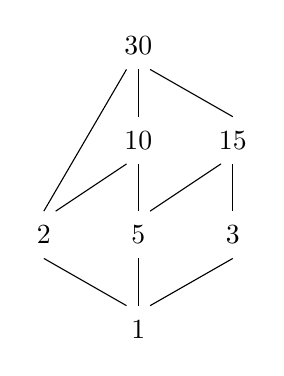
\begin{tikzpicture}[scale=0.6] %Replaced figure with tikz figure - TWJ 8/22/2010

\draw (0,0.5) -- (0,1.5);
\draw (0,2.5) -- (0,3.5);
\draw (2,2.5) -- (2,3.5);
\draw (0,4.5) -- (0,5.5);

\draw (0.25,5.5) -- (2,4.5);
\draw (-0.25,5.5) -- (-2,2.5);

\draw (1.75,3.5) -- (0.25,2.5);
\draw (-0.25,3.5) -- (-1.75,2.5);

\draw (2,1.5) -- (0.25,0.5);
\draw (-2,1.5) -- (-0.25,0.5);

\node at (0,6) {30};
\node at (0,4) {10};
\node at (2,4) {15};
\node at (-2, 2) {2};
\node at (0, 2) {5};
\node at (2, 2) {3};
\node at (0, 0) {1};

\end{tikzpicture}
\end{center}
 
 
 
\item[5.] 
False.
 

 
\item[6.]
(a) $(a \vee b \vee a') \wedge a$.
\begin{center}  
\tikzpreface{solution_circuit_a}
\begin{tikzpicture}[scale=0.8,node distance=5mm, text height=1.5ex,text depth=.25ex] %Replaced figure with tikz figure - TWJ 8/22/2010

\draw  (0,0) -- (2.2,0) (2.8,0) -- (4.7,0)  (5.3,0) -- (6,0);
\draw  (1,0) -- (1,1) -- (2.2,1)  (2.8,1) -- (4,1) -- (4,0);
\draw  (1,0) -- (1,-1) -- (2.2,-1)  (2.8,-1) -- (4,-1) -- (4,0);

\node at (2.5,-1) {$a'$};
\node at (2.5,0) {$b$};
\node at (2.5,1) {$a$};
\node at (5,0) {$a$};



\end{tikzpicture}
\end{center}
 


(c) $a \vee (a \wedge b)$.
\begin{center}  

\tikzpreface{solution_circuit_c}
\begin{tikzpicture}[scale=0.8,node distance=5mm, text height=1.5ex,text depth=.25ex] %Replaced figure with tikz figure - TWJ 8/22/2010

\draw  (0,0) -- (1,0) (4,0) -- (5,0);
\draw  (1,0) -- (1,1) -- (1.7,1)  (2.3,1) -- (2.7,1)  (3.3,1) -- (4,1) -- (4,0);
\draw  (1,0) -- (1,-1) -- (2.2,-1)  (2.8,-1) -- (4,-1) -- (4,0);

\node at (2.5,-1) {$a$};
\node at (2,1) {$a$};
\node at (3,1) {$b$};



\end{tikzpicture}
\end{center}
 
 
 
 
\item[8.]
Not equivalent.
 
\item[10.]
$a' \wedge [(a \wedge b') \vee b] = a \wedge (a \vee b)$.

\item[15.]
Let $I, J$ be ideals in $R$. We need to show that $I + J 
= \{ r + s : r \in
I \mbox{ and } s \in J  \}$ is the smallest ideal in $R$ containing
both $I$ and $J$. If $r_1, r_2 \in I$ and $s_1, s_2 \in J$, then
$(r_1 + s_1) + (r_2 + s_2) = (r_1 + r_2) +(s_1 + s_2)$ is in $I + J$.
For $a \in R$, $a(r_1 + s_1) = ar_1 + as_1 \in I + J$; hence, $I + J$
is an ideal in $R$.


\item[19.]
(a) No.

\item[21.]
$( \Rightarrow)$. $a = b \Rightarrow (a \wedge b') \vee (a' \wedge b)
= (a \wedge a') \vee (a' \wedge a) = O \vee O = O$. \\
$( \Leftarrow)$. $( a \wedge b') \vee (	a' \wedge b) = O \Rightarrow
a \vee b = (a \vee a) \vee b = a \vee (a \vee b) = a \vee [I \wedge
(a \vee b)] = a \vee [(a \vee a') \wedge (a \vee b)] = [a \vee
(a \wedge b')] \vee [a \vee (a' \wedge b)] = a \vee [(a \wedge b') \vee
(a' \wedge b)] = a \vee 0 = a$.  A symmetric argument shows that $a
\vee b = b$.



 
\end{itemize}
}
 
\subsection*{Chapter 20. Vector Spaces}
 
{\small
\begin{itemize}
 
\item[3.] 
${\mathbb Q}(\sqrt{2}, \sqrt{3}\, )$ has basis $\{ 1, \sqrt{2}, \sqrt{3},
\sqrt{6}\, \}$  over ${\mathbb Q}$.
 
\item[5.]
$P_n$ has basis $\{ 1, x, x^2, \ldots, x^{n-1} \}$.
 
\item[7.]
(a) Subspace of dimension 2 with basis $\{(1, 0, -3), (0, 1,
2) \}$.\\
(d) Not a subspace.
 
\item[10.]
$0 =  \alpha 0 = \alpha(-v+v) = \alpha(-v) + \alpha v \Rightarrow 
-\alpha v = \alpha(-v)$.
 
\item[12.]
Let $v_0 = 0, v_1, \ldots, v_n \in V$ and $\alpha_0 \neq 0, \alpha_1,
\ldots, \alpha_n \in F$. Then $\alpha_0 v_0 + \cdots + \alpha_n v_n =
0$.
 
\item[15.]
(a)
Let $u, v \in \ker(T)$ and $\alpha \in F$.  Then
\[
\begin{array}{c}
T(u +v) = T(u) + T(v) = 0 \\
T(\alpha v) = \alpha T(v) = \alpha 0 = 0.
\end{array}
\]
Hence, $u + v, \alpha v \in \ker(T) \Rightarrow \ker(T)$ is 
a subspace of
$V$. \\
(c) 
$T(u) = T(v) \Leftrightarrow T(u-v) = T(u) - T(v) = 0
\Leftrightarrow u-v = 0 \Leftrightarrow u = v$.
 
 
\item[17.]
(a)
Let $u, u' \in U$ and $v, v' \in V$. Then
\[
\begin{array}{c}
(u + v) + (u' + v') = (u + u') + (v + v') \in U + V \\
\alpha(u + v) = \alpha u + \alpha v \in U + V.
\end{array}
\]
 
\end{itemize}
}
 
\subsection*{Chapter 21. Fields}
 
{\small
\begin{itemize}
 
\item[1.] 
(a) $x^4 -\frac{2}{3} x^2 - \frac{62}{9}$.
(c) $x^4 - 2 x^2 + 25$.
 
\item[2.] 
(a) $\{ 1, \sqrt{2}, \sqrt{3}, \sqrt{6}\, \}$.
(c) $\{ 1, i, \sqrt{2}, \sqrt{2}\, i \}$.
(e) $\{1, 2^{1/6}, 2^{1/3}, 2^{1/2}, 2^{2/3}, 2^{5/6}  \}$.
 
\item[3.]
(a) ${\mathbb Q}(\sqrt{3}, \sqrt{7}\, )$.
 

\item[5.]
Use the fact that the elements of ${\mathbb Z}_2[x]/ \langle x^3 + x +
1\rangle$ are 0, 1, $\alpha$, $1 + \alpha$, $\alpha^2$, $1 + \alpha^2$,
$\alpha + \alpha^2$, $1 + \alpha + \alpha^2$ and the fact that
$\alpha^3 + \alpha + 1 = 0$. 


\item[8.]
False.


\item[14.]
Suppose that $E$ is algebraic over $F$ and $K$ is
algebraic over $E$. Let $\alpha \in K$. It suffices to show that
$\alpha$ is algebraic over some finite extension of $F$. Since
$\alpha$ is algebraic over $E$, it must be the zero of some polynomial
$p(x) = \beta_0 + \beta_1 x + \cdots + \beta_n x^n$ in $E[x]$. Hence
$\alpha$ is algebraic over $F(\beta_0, \ldots, \beta_n)$.


\item[22.]
${\mathbb Q}( \sqrt{3}, \sqrt{7}\, ) \supset {\mathbb Q}( \sqrt{3} +\sqrt{7}\,
)$ since $\{ 1, \sqrt{3}, \sqrt{7}, \sqrt{21}\, \}$ is a basis for
${\mathbb Q}( \sqrt{3}, \sqrt{7}\, )$ over ${\mathbb Q}$. Since $[{\mathbb Q}(
\sqrt{3}, \sqrt{7}\, ) : {\mathbb Q}] = 4$, $[{\mathbb Q}( \sqrt{3}
+\sqrt{7}\, ) : {\mathbb Q}] = 2$ or 4. Since the degree of the minimal
polynomial of $\sqrt{3} +\sqrt{7}$ is 4, ${\mathbb Q}( \sqrt{3},
\sqrt{7}\, ) = {\mathbb Q}( \sqrt{3} +\sqrt{7}\, )$.


\item[27.]
Let $\beta \in F(\alpha)$ not in $F$. Then $\beta =
p(\alpha)/q(\alpha)$, where $p$ and $q$ are polynomials in $\alpha$
with $q(\alpha) \neq 0$ and coefficients in $F$. If $\beta$ is
algebraic over $F$, then there exists a polynomial $f(x) \in F[x]$
such that $f(\beta) = 0$. Let $f(x) = a_0 + a_1 x + \cdots + a_n x^n$.
Then  
\[
0 = f(\beta) = f\left( 
\frac{p(\alpha)}{q(\alpha)} \right)
= a_0 + a_1 \left( \frac{p(\alpha)}{q(\alpha)} \right)  + \cdots + a_n
\left( \frac{p(\alpha)}{q(\alpha)} \right)^n. 
\]
Now multiply both sides by $q(\alpha)^n$ to show that there is a
polynomial in $F[x]$ that has $\alpha$ as a zero.




\end{itemize}
}
 
\subsection*{Chapter 22. Finite Fields}
 
{\small
\begin{itemize}

\item[1.]
(a) 2.
(c) 2.
 
\item[4.] 
There are eight elements in ${\mathbb Z}_2(\alpha)$. Exhibit two more
zeros of $x^3 + x^2 + 1$ other than $\alpha$ in these eight elements. 
 
\item[5.] 
Find an irreducible polynomial $p(x)$ in ${\mathbb Z}_3[x]$ of degree
3 and show that ${\mathbb Z}_3[x]/ \langle p(x) \rangle$ has 27
elements. 

\item[7.]
(a) $x^5 -1 = (x+1)(x^4+x^3 + x^2 + x+ 1)$. \\
(c) $x^9 -1 = (x+1)( x^2 + x+ 1)(x^6+x^3+1)$.
 
\item[8.]
True.

\item[11.]
(a) Use the fact that $x^7 -1 = (x+1)( x^3 + x+ 1)(x^3+x^2+1)$.

\item[12.]
False.

\item[17.]
If $p(x) \in F[x]$, then $p(x) \in E[x]$.


\item[18.]
Since $\alpha$ is algebraic over $F$ of degree $n$, we can write any
element $\beta \in F(\alpha)$ uniquely as $\beta = a_0  + a_1 \alpha +
\cdots + a_{n-1} \alpha^{n-1}$ with $a_i \in F$. There are $q^n$
possible $n$-tuples $(a_0, a_1, \ldots, a_{n-1})$.


\item[24.]
Factor $x^{p-1} - 1$ over ${\mathbb Z}_p$.


\end{itemize}
}
 
\subsection*{Chapter 23. Galois Theory}
 
{\small
\begin{itemize}
 
\item[1.]
(a) ${\mathbb Z}_2$.
(c) ${\mathbb Z}_2 \times {\mathbb Z}_2 \times {\mathbb Z}_2$.
 
\item[2.]
(a) Separable.
(c) Not separable.
 
\item[3.]
$[{\rm GF}(729): {\rm GF}(9)] = [{\rm GF}(729): {\rm GF}(3)] /[{\rm
GF}(9): {\rm GF}(3)] = 6/2 = 3 \Rightarrow G({\rm GF}(729)/ {\rm
GF}(9)) \cong {\mathbb Z}_3$. A generator for $G({\rm GF}(729)/ {\rm
GF}(9))$ is $\sigma$, where $\sigma_{3^6}( \alpha) = \alpha^{3^6} =
\alpha^{729}$ for $\alpha \in {\rm GF}(729)$.

\item[4.]
(a) $S_5$.
(c) $S_3$.

\item[5.]
(a) ${\mathbb Q}(i)$.


\item[7.]
Let $E$ be the splitting field of a cubic polynomial in $F[x]$. Show that
\mbox{$[E:F]$} is less than or equal to 6 and is divisible by 3. Since $G(E/F)$ is a subgroup of
$S_3$ whose order is divisible by 3, conclude that this group must be 
isomorphic to ${\mathbb Z}_3$ or $S_3$.
 
\item[9.]
$G$ is a subgroup of $S_n$.

\item[16.]
True.

\item[20.]
(a) Clearly $\omega, \omega^2, \ldots, \omega^{p-1}$ are
distinct since $\omega \neq 1$ or 0. To show that $\omega^i$ is a zero
of $\Phi_p$, calculate $\Phi_p( \omega^i)$. \\
(b) The conjugates of $\omega$ are $\omega, \omega^2, \ldots,
\omega^{p-1}$. Define a map  $\phi_i: {\mathbb Q}(\omega)
\rightarrow {\mathbb Q}(\omega^i)$ by 
\[
\phi_i(a_0 + a_1 \omega +
\cdots + a_{p-2} \omega^{p-2}) = a_0 + a_1 \omega^i + \cdots + c_{p-2} 
(\omega^i)^{p-2},
\]
where $a_i \in {\mathbb Q}$. Prove that $\phi_i$ is an isomorphism of
fields. Show that $\phi_2$ 
generates $G({\mathbb Q}(\omega)/{\mathbb Q})$. \\ 
(c)
Show that $\{ \omega, \omega^2, \ldots, \omega^{p-1} \}$ is a basis
for ${\mathbb Q}( \omega )$ over ${\mathbb Q}$, and consider which linear
combinations of $\omega, \omega^2, \ldots, \omega^{p-1}$ are left
fixed by all elements of $G( {\mathbb Q}( \omega ) / {\mathbb Q})$.
 
 
 
\end{itemize}
}
 
 
 
 
\pagestyle{headings}
 
 
 
 

{\small%%%%(c)
%%%%(c)  This file is a portion of the source for the textbook
%%%%(c)
%%%%(c)    Abstract Algebra: Theory and Applications
%%%%(c)    Copyright 1997 by Thomas W. Judson
%%%%(c)
%%%%(c)  See the file COPYING.txt for copying conditions
%%%%(c)
%%%%(c)
\chapter*{GNU Free Documentation License}

\addcontentsline{toc}{chapter}{GNU Free Documentation License}
\pagestyle{myheadings}
\markboth{GFDL LICENSE}{GFDL LICENSE}

 \begin{center}

       Version 1.2, November 2002

%% RAB, 2010/07/21
%% Copyright symbol ("\copyright") causes trouble in xhtml/jsmath conversion
 Copyright 2000,2001,2002  Free Software Foundation, Inc.
 
 \bigskip
 
     51 Franklin St, Fifth Floor, Boston, MA  02110-1301  USA
  
 \bigskip
 
 Everyone is permitted to copy and distribute verbatim copies
 of this license document, but changing it is not allowed.
\end{center}


\begin{center}
\textbf{\large Preamble}
\end{center}

The purpose of this License is to make a manual, textbook, or other
functional and useful document ``free'' in the sense of freedom: to
assure everyone the effective freedom to copy and redistribute it,
with or without modifying it, either commercially or noncommercially.
Secondarily, this License preserves for the author and publisher a way
to get credit for their work, while not being considered responsible
for modifications made by others.

This License is a kind of ``copyleft'', which means that derivative
works of the document must themselves be free in the same sense.  It
complements the GNU General Public License, which is a copyleft
license designed for free software.

We have designed this License in order to use it for manuals for free
software, because free software needs free documentation: a free
program should come with manuals providing the same freedoms that the
software does.  But this License is not limited to software manuals;
it can be used for any textual work, regardless of subject matter or
whether it is published as a printed book.  We recommend this License
principally for works whose purpose is instruction or reference.

\section*{1.\ Applicability And Definitions}
% \begin{center}
% {\Large\bf 1. APPLICABILITY AND DEFINITIONS\par}
% \phantomsection
% \addcontentsline{toc}{section}{1. APPLICABILITY AND DEFINITIONS}
% \end{center}

This License applies to any manual or other work, in any medium, that
contains a notice placed by the copyright holder saying it can be
distributed under the terms of this License.  Such a notice grants a
world-wide, royalty-free license, unlimited in duration, to use that
work under the conditions stated herein.  The ``\textbf{Document}'', below,
refers to any such manual or work.  Any member of the public is a
licensee, and is addressed as ``\textbf{you}''.  You accept the license if you
copy, modify or distribute the work in a way requiring permission
under copyright law.

A ``\textbf{Modified Version}'' of the Document means any work containing the
Document or a portion of it, either copied verbatim, or with
modifications and/or translated into another language.

A ``\textbf{Secondary Section}'' is a named appendix or a front-matter section of
the Document that deals exclusively with the relationship of the
publishers or authors of the Document to the Document's overall subject
(or to related matters) and contains nothing that could fall directly
within that overall subject.  (Thus, if the Document is in part a
textbook of mathematics, a Secondary Section may not explain any
mathematics.)  The relationship could be a matter of historical
connection with the subject or with related matters, or of legal,
commercial, philosophical, ethical or political position regarding
them.

The ``\textbf{Invariant Sections}'' are certain Secondary Sections whose titles
are designated, as being those of Invariant Sections, in the notice
that says that the Document is released under this License.  If a
section does not fit the above definition of Secondary then it is not
allowed to be designated as Invariant.  The Document may contain zero
Invariant Sections.  If the Document does not identify any Invariant
Sections then there are none.

The ``\textbf{Cover Texts}'' are certain short passages of text that are listed,
as Front-Cover Texts or Back-Cover Texts, in the notice that says that
the Document is released under this License.  A Front-Cover Text may
be at most 5 words, and a Back-Cover Text may be at most 25 words.

A ``\textbf{Transparent}'' copy of the Document means a machine-readable copy,
represented in a format whose specification is available to the
general public, that is suitable for revising the document
straightforwardly with generic text editors or (for images composed of
pixels) generic paint programs or (for drawings) some widely available
drawing editor, and that is suitable for input to text formatters or
for automatic translation to a variety of formats suitable for input
to text formatters.  A copy made in an otherwise Transparent file
format whose markup, or absence of markup, has been arranged to thwart
or discourage subsequent modification by readers is not Transparent.
An image format is not Transparent if used for any substantial amount
of text.  A copy that is not ``Transparent'' is called ``\textbf{Opaque}''.

Examples of suitable formats for Transparent copies include plain
ASCII without markup, Texinfo input format, LaTeX input format, SGML
or XML using a publicly available DTD, and standard-conforming simple
HTML, PostScript or PDF designed for human modification.  Examples of
transparent image formats include PNG, XCF and JPG.  Opaque formats
include proprietary formats that can be read and edited only by
proprietary word processors, SGML or XML for which the DTD and/or
processing tools are not generally available, and the
machine-generated HTML, PostScript or PDF produced by some word
processors for output purposes only.

The ``\textbf{Title Page}'' means, for a printed book, the title page itself,
plus such following pages as are needed to hold, legibly, the material
this License requires to appear in the title page.  For works in
formats which do not have any title page as such, ``Title Page'' means
the text near the most prominent appearance of the work's title,
preceding the beginning of the body of the text.

A section ``\textbf{Entitled XYZ}'' means a named subunit of the Document whose
title either is precisely XYZ or contains XYZ in parentheses following
text that translates XYZ in another language.  (Here XYZ stands for a
specific section name mentioned below, such as ``\textbf{Acknowledgements}'',
``\textbf{Dedications}'', ``\textbf{Endorsements}'', or ``\textbf{History}''.)  
To ``\textbf{Preserve the Title}''
of such a section when you modify the Document means that it remains a
section ``Entitled XYZ'' according to this definition.

The Document may include Warranty Disclaimers next to the notice which
states that this License applies to the Document.  These Warranty
Disclaimers are considered to be included by reference in this
License, but only as regards disclaiming warranties: any other
implication that these Warranty Disclaimers may have is void and has
no effect on the meaning of this License.

\section*{2.\ Verbatim Copying}
% \begin{center}
% {\Large\bf 2. VERBATIM COPYING\par}
% %% \phantomsection
% \addcontentsline{toc}{section}{2. VERBATIM COPYING}
% \end{center}

You may copy and distribute the Document in any medium, either
commercially or noncommercially, provided that this License, the
copyright notices, and the license notice saying this License applies
to the Document are reproduced in all copies, and that you add no other
conditions whatsoever to those of this License.  You may not use
technical measures to obstruct or control the reading or further
copying of the copies you make or distribute.  However, you may accept
compensation in exchange for copies.  If you distribute a large enough
number of copies you must also follow the conditions in section~3.

You may also lend copies, under the same conditions stated above, and
you may publicly display copies.

\section*{3.\ Copying In Quantity}
% \begin{center}
% {\Large\bf 3. COPYING IN QUANTITY\par}
% %% \phantomsection
% \addcontentsline{toc}{section}{3. COPYING IN QUANTITY}
% \end{center}


If you publish printed copies (or copies in media that commonly have
printed covers) of the Document, numbering more than 100, and the
Document's license notice requires Cover Texts, you must enclose the
copies in covers that carry, clearly and legibly, all these Cover
Texts: Front-Cover Texts on the front cover, and Back-Cover Texts on
the back cover.  Both covers must also clearly and legibly identify
you as the publisher of these copies.  The front cover must present
the full title with all words of the title equally prominent and
visible.  You may add other material on the covers in addition.
Copying with changes limited to the covers, as long as they preserve
the title of the Document and satisfy these conditions, can be treated
as verbatim copying in other respects.

If the required texts for either cover are too voluminous to fit
legibly, you should put the first ones listed (as many as fit
reasonably) on the actual cover, and continue the rest onto adjacent
pages.

If you publish or distribute Opaque copies of the Document numbering
more than 100, you must either include a machine-readable Transparent
copy along with each Opaque copy, or state in or with each Opaque copy
a computer-network location from which the general network-using
public has access to download using public-standard network protocols
a complete Transparent copy of the Document, free of added material.
If you use the latter option, you must take reasonably prudent steps,
when you begin distribution of Opaque copies in quantity, to ensure
that this Transparent copy will remain thus accessible at the stated
location until at least one year after the last time you distribute an
Opaque copy (directly or through your agents or retailers) of that
edition to the public.

It is requested, but not required, that you contact the authors of the
Document well before redistributing any large number of copies, to give
them a chance to provide you with an updated version of the Document.

\section*{4.\ Modifications}
% \begin{center}
% {\Large\bf 4. MODIFICATIONS\par}
% %% \phantomsection
% \addcontentsline{toc}{section}{4. MODIFICATIONS}
% \end{center}

You may copy and distribute a Modified Version of the Document under
the conditions of sections 2 and 3 above, provided that you release
the Modified Version under precisely this License, with the Modified
Version filling the role of the Document, thus licensing distribution
and modification of the Modified Version to whoever possesses a copy
of it.  In addition, you must do these things in the Modified Version:

\begin{itemize}
\item[A.] 
   Use in the Title Page (and on the covers, if any) a title distinct
   from that of the Document, and from those of previous versions
   (which should, if there were any, be listed in the History section
   of the Document).  You may use the same title as a previous version
   if the original publisher of that version gives permission.
   
\item[B.]
   List on the Title Page, as authors, one or more persons or entities
   responsible for authorship of the modifications in the Modified
   Version, together with at least five of the principal authors of the
   Document (all of its principal authors, if it has fewer than five),
   unless they release you from this requirement.
   
\item[C.]
   State on the Title page the name of the publisher of the
   Modified Version, as the publisher.
   
\item[D.]
   Preserve all the copyright notices of the Document.
   
\item[E.]
   Add an appropriate copyright notice for your modifications
   adjacent to the other copyright notices.
   
\item[F.]
   Include, immediately after the copyright notices, a license notice
   giving the public permission to use the Modified Version under the
   terms of this License, in the form shown in the Addendum below.
   
\item[G.]
   Preserve in that license notice the full lists of Invariant Sections
   and required Cover Texts given in the Document's license notice.
   
\item[H.]
   Include an unaltered copy of this License.
   
\item[I.]
   Preserve the section Entitled ``History'', Preserve its Title, and add
   to it an item stating at least the title, year, new authors, and
   publisher of the Modified Version as given on the Title Page.  If
   there is no section Entitled ``History'' in the Document, create one
   stating the title, year, authors, and publisher of the Document as
   given on its Title Page, then add an item describing the Modified
   Version as stated in the previous sentence.
   
\item[J.]
   Preserve the network location, if any, given in the Document for
   public access to a Transparent copy of the Document, and likewise
   the network locations given in the Document for previous versions
   it was based on.  These may be placed in the ``History'' section.
   You may omit a network location for a work that was published at
   least four years before the Document itself, or if the original
   publisher of the version it refers to gives permission.
   
\item[K.]
   For any section Entitled ``Acknowledgements'' or ``Dedications'',
   Preserve the Title of the section, and preserve in the section all
   the substance and tone of each of the contributor acknowledgements
   and/or dedications given therein.
   
\item[L.]
   Preserve all the Invariant Sections of the Document,
   unaltered in their text and in their titles.  Section numbers
   or the equivalent are not considered part of the section titles.
   
\item[M.]
   Delete any section Entitled ``Endorsements''.  Such a section
   may not be included in the Modified Version.
   
\item[N.]
   Do not retitle any existing section to be Entitled ``Endorsements''
   or to conflict in title with any Invariant Section.
   
\item[O.]
   Preserve any Warranty Disclaimers.
\end{itemize}

If the Modified Version includes new front-matter sections or
appendices that qualify as Secondary Sections and contain no material
copied from the Document, you may at your option designate some or all
of these sections as invariant.  To do this, add their titles to the
list of Invariant Sections in the Modified Version's license notice.
These titles must be distinct from any other section titles.

You may add a section Entitled ``Endorsements'', provided it contains
nothing but endorsements of your Modified Version by various
parties--for example, statements of peer review or that the text has
been approved by an organization as the authoritative definition of a
standard.

You may add a passage of up to five words as a Front-Cover Text, and a
passage of up to 25 words as a Back-Cover Text, to the end of the list
of Cover Texts in the Modified Version.  Only one passage of
Front-Cover Text and one of Back-Cover Text may be added by (or
through arrangements made by) any one entity.  If the Document already
includes a cover text for the same cover, previously added by you or
by arrangement made by the same entity you are acting on behalf of,
you may not add another; but you may replace the old one, on explicit
permission from the previous publisher that added the old one.

The author(s) and publisher(s) of the Document do not by this License
give permission to use their names for publicity for or to assert or
imply endorsement of any Modified Version.

\section*{5.\ Combining Documents}
% \begin{center}
% {\Large\bf 5. COMBINING DOCUMENTS\par}
% %% \phantomsection
% \addcontentsline{toc}{section}{5. COMBINING DOCUMENTS}
% \end{center}


You may combine the Document with other documents released under this
License, under the terms defined in section~4 above for modified
versions, provided that you include in the combination all of the
Invariant Sections of all of the original documents, unmodified, and
list them all as Invariant Sections of your combined work in its
license notice, and that you preserve all their Warranty Disclaimers.

The combined work need only contain one copy of this License, and
multiple identical Invariant Sections may be replaced with a single
copy.  If there are multiple Invariant Sections with the same name but
different contents, make the title of each such section unique by
adding at the end of it, in parentheses, the name of the original
author or publisher of that section if known, or else a unique number.
Make the same adjustment to the section titles in the list of
Invariant Sections in the license notice of the combined work.

In the combination, you must combine any sections Entitled ``History''
in the various original documents, forming one section Entitled
``History''; likewise combine any sections Entitled ``Acknowledgements'',
and any sections Entitled ``Dedications''.  You must delete all sections
Entitled ``Endorsements''.

\section*{6.\ Collections Of Documents}
% \begin{center}
% {\Large\bf 6. COLLECTIONS OF DOCUMENTS\par}
% %% \phantomsection
% \addcontentsline{toc}{section}{6. COLLECTIONS OF DOCUMENTS}
% \end{center}

You may make a collection consisting of the Document and other documents
released under this License, and replace the individual copies of this
License in the various documents with a single copy that is included in
the collection, provided that you follow the rules of this License for
verbatim copying of each of the documents in all other respects.

You may extract a single document from such a collection, and distribute
it individually under this License, provided you insert a copy of this
License into the extracted document, and follow this License in all
other respects regarding verbatim copying of that document.

\section*{7.\ Aggregation With Independent Works}
% \begin{center}
% {\Large\bf 7. AGGREGATION WITH INDEPENDENT WORKS\par}
% %% \phantomsection
% \addcontentsline{toc}{section}{7. AGGREGATION WITH INDEPENDENT WORKS}
% \end{center}


A compilation of the Document or its derivatives with other separate
and independent documents or works, in or on a volume of a storage or
distribution medium, is called an ``aggregate'' if the copyright
resulting from the compilation is not used to limit the legal rights
of the compilation's users beyond what the individual works permit.
When the Document is included in an aggregate, this License does not
apply to the other works in the aggregate which are not themselves
derivative works of the Document.

If the Cover Text requirement of section~3 is applicable to these
copies of the Document, then if the Document is less than one half of
the entire aggregate, the Document's Cover Texts may be placed on
covers that bracket the Document within the aggregate, or the
electronic equivalent of covers if the Document is in electronic form.
Otherwise they must appear on printed covers that bracket the whole
aggregate.

\section*{8.\ Translation}
% \begin{center}
% {\Large\bf 8. TRANSLATION\par}
% %% \phantomsection
% \addcontentsline{toc}{section}{8. TRANSLATION}
% \end{center}


Translation is considered a kind of modification, so you may
distribute translations of the Document under the terms of section~4.
Replacing Invariant Sections with translations requires special
permission from their copyright holders, but you may include
translations of some or all Invariant Sections in addition to the
original versions of these Invariant Sections.  You may include a
translation of this License, and all the license notices in the
Document, and any Warranty Disclaimers, provided that you also include
the original English version of this License and the original versions
of those notices and disclaimers.  In case of a disagreement between
the translation and the original version of this License or a notice
or disclaimer, the original version will prevail.

If a section in the Document is Entitled ``Acknowledgements'',
``Dedications'', or ``History'', the requirement (section~4) to Preserve
its Title (section~1) will typically require changing the actual
title.

\section*{9.\ Termination}
% \begin{center}
% {\Large\bf 9. TERMINATION\par}
% %% \phantomsection
% \addcontentsline{toc}{section}{9. TERMINATION}
% \end{center}


You may not copy, modify, sublicense, or distribute the Document except
as expressly provided for under this License.  Any other attempt to
copy, modify, sublicense or distribute the Document is void, and will
automatically terminate your rights under this License.  However,
parties who have received copies, or rights, from you under this
License will not have their licenses terminated so long as such
parties remain in full compliance.

\section*{10.\ Future Revisions Of This License}
% \begin{center}
% {\Large\bf 10. FUTURE REVISIONS OF THIS LICENSE\par}
% %% \phantomsection
% \addcontentsline{toc}{section}{10. FUTURE REVISIONS OF THIS LICENSE}
% \end{center}


The Free Software Foundation may publish new, revised versions
of the GNU Free Documentation License from time to time.  Such new
versions will be similar in spirit to the present version, but may
differ in detail to address new problems or concerns.  See
http://www.gnu.org/copyleft/.

Each version of the License is given a distinguishing version number.
If the Document specifies that a particular numbered version of this
License ``or any later version'' applies to it, you have the option of
following the terms and conditions either of that specified version or
of any later version that has been published (not as a draft) by the
Free Software Foundation.  If the Document does not specify a version
number of this License, you may choose any version ever published (not
as a draft) by the Free Software Foundation.

\section*{Addendum: How to use this License for your documents}
% \begin{center}
% {\Large\bf ADDENDUM: How to use this License for your documents\par}
% %% \phantomsection
% \addcontentsline{toc}{section}{ADDENDUM: How to use this License for your documents}
% \end{center}

To use this License in a document you have written, include a copy of
the License in the document and put the following copyright and
license notices just after the title page:

%% RAB, 2010/07/21
%% Copyright symbol ("\copyright") causes trouble in xhtml/jsmath conversion
\bigskip
\begin{quote}
    Copyright  YEAR  YOUR NAME.
    Permission is granted to copy, distribute and/or modify this document
    under the terms of the GNU Free Documentation License, Version 1.2
    or any later version published by the Free Software Foundation;
    with no Invariant Sections, no Front-Cover Texts, and no Back-Cover Texts.
    A copy of the license is included in the section entitled ``GNU
    Free Documentation License''.
\end{quote}
\bigskip
    
If you have Invariant Sections, Front-Cover Texts and Back-Cover Texts,
replace the ``with \dots\ Texts.'' line with this:

\bigskip
\begin{quote}
    with the Invariant Sections being LIST THEIR TITLES, with the
    Front-Cover Texts being LIST, and with the Back-Cover Texts being LIST.
\end{quote}
\bigskip
    
If you have Invariant Sections without Cover Texts, or some other
combination of the three, merge those two alternatives to suit the
situation.

If your document contains nontrivial examples of program code, we
recommend releasing these examples in parallel under your choice of
free software license, such as the GNU General Public License,
to permit their use in free software.
}
%%%%(c)
%%%%(c)  This file is a portion of the source for the textbook
%%%%(c)
%%%%(c)    Abstract Algebra: Theory and Applications
%%%%(c)    Copyright 1997 by Thomas W. Judson
%%%%(c)
%%%%(c)  See the file COPYING.txt for copying conditions
%%%%(c)
%%%%(c)
\chapter*{Notation}

% Print versions need page headers, ToC entry
% tex4ht versions get their own ToC automatically
\ifthenelse{\boolean{basic}}{%
\phantomsection
\addcontentsline{toc}{chapter}{Notation}
\pagestyle{myheadings}
\markboth{NOTATION}{NOTATION}
}{}

The following table defines the  notation used in this book. Page numbers
refer to the first appearance of each symbol.
%
\begin{center}
\begin{longtable}{llr}
%
\multicolumn{1}{l}\textbf{Symbol} & \multicolumn{1}{l}\textbf{Description} & \multicolumn{1}{r}\textbf{Page} \\
&&\\
\endfirsthead
%
\multicolumn{1}{l}\textbf{Symbol} & \multicolumn{1}{l}\textbf{Description} & \multicolumn{1}{r}\textbf{Page} \\
&&\\
\endhead
%
$a \in A$ & $a$ is in the set $A$ & \pageref{sets_membership} \\
%
${\mathbb N}$ & the natural numbers & \pageref{naturalnum} \\
%
${\mathbb Z}$ & the integers & \pageref{sets_integers} \\
%
${\mathbb Q}$ & the rational numbers & \pageref{rationals} \\
%
${\mathbb R}$ & the real numbers & \pageref{reals} \\
%
${\mathbb C}$ & the complex numbers & \pageref{complexnum} \\
%
$A \subset B$ & $A$ is a subset of $B$ & \pageref{setcontain} \\
%
$\emptyset$ & the empty set & \pageref{theemptyset} \\
%
$A \cup B$ & union of sets $A$ and $B$ & \pageref{union} \\
%
$A \cap B$ & intersection of sets $A$ and $B$ & \pageref{intersection} \\
%
$A'$ & complement of the  set $A$ & \pageref{setcomplement} \\
%
$A \setminus B$ & difference between sets $A$ and $B$ & \pageref{setdifference} \\
%
$A \times B$ & Cartesian product of sets $A$ and $B$ & \pageref{cartesian} \\
%
$A^n$ & $A \times \cdots \times A$ ($n$ times) & \pageref{ncartesian} \\
%
$id$ & identity mapping & \pageref{noteidentity} \\
%
$f^{-1}$ & inverse of the function $f$	& \pageref{inversefunc} \\
%
$a \equiv b \pmod{n}$ & $a$ is congruent to $b$ modulo $n$ & \pageref{amodb} \\
%
$n!$ & $n$ factorial & \pageref{factorial} \\
%
$\left(\begin{array}{c}n \\ k \end{array} \right)$ & binomial coefficient $n!/(k! (n-k)!)$ & \pageref{binomial} \\
%
$m \mid n$ & $m$ divides $n$ & \pageref{divides} \\
%
$\gcd(m, n)$ & greatest common divisor of $m$ and $n$ & \pageref{greatestcd}\\
%
${\cal P}(X)$ & power set of $X$ & \pageref{powerset} \\
%
${\mathbb Z}_n$ & the integers modulo $n$ & \pageref{integersmodn} \\
%
$\lcm(m,n)$ & least common multiple of $m$ and $n$ & \pageref{leastcm} \\
%
$U(n)$ & group of units in ${\mathbb Z}_n$ & \pageref{groupofunits} \\
%
${\mathbb M}_n ( {\mathbb R})$ & the $n \times n$ matrices with entries in ${\mathbb R}$ &  \pageref{notematrices} \\
%
$\det A$ & determinant of $A$ & \pageref{determinant} \\
%
$GL_n({\mathbb R})$ & general linear group & \pageref{generallinear} \\
%
$Q_8$ & the group of quaternions & \pageref{notequateriongroup} \\
%
${\mathbb C}^\ast$ & the multiplicative group of complex numbers & \pageref{noteCstar} \\
%
$|G|$ & order of a group $G$ & \pageref{noteorder} \\
%
${\mathbb R}^*$ & the multiplicative group of real numbers & \pageref{noteRstar} \\
%
${\mathbb Q}^*$ & the multiplicative group of rational numbers & \pageref{noteQstar} \\
%
$SL_n({\mathbb R})$ & special linear group & \pageref{speciallinear} \\
%
$Z(G)$ & center of a group $G$ & \pageref{centerofagroup} \\
%
$\langle a \rangle$ & cyclic subgroup generated by $a$ & \pageref{generatedby} \\
%
$|a|$ & order of an element $a$ & \pageref{noteelementorder} \\
%
$\cis \theta$ & $\cos \theta + i \sin \theta$ & \pageref{cosisin} \\
%
${\mathbb T}$ & the circle group & \pageref{notecirclegroup} \\
%
$S_n$ & symmetric group on $n$ letters & \pageref{symmetricgroup} \\
%
$(a_1, a_2, \ldots, a_k )$ & cycle of length $k$ & \pageref{notecycle} \\
%
$A_n$ & alternating group on $n$ letters & \pageref{alternatinggroup} \\
%
$D_n$ & dihedral group & \pageref{dihedralgroup} \\
%
$[G:H]$ & index of a subgroup $H$ in a group $G$ & \pageref{indexofasubgroup}  \\
%
${\cal L}_H$ & set of left cosets of $H$ in a group $G$ & \pageref{notesetleft} \\
%
${\cal R}_H$ & set of right cosets of $H$ in a group $G$ & \pageref{notesetright}  \\
%
$d({\mathbf x}, {\mathbf y})$ & Hamming distance between ${\mathbf x}$ and ${\mathbf y}$ & \pageref{noteHammingdist} \\
%
$d_{\min}$ & minimum distance of a code & \pageref{notemindist}\\
%
$w({\mathbf x})$ & weight of ${\mathbf x}$ & \pageref{noteweight} \\
%
${\mathbb M}_{m \times n}({\mathbb Z}_2)$ & set of $m$ by $n$ matrices with entries in ${\mathbb Z}_2$ & \pageref{notembyn} \\
%
${\rm Null}(H)$ & null space of a matrix $H$ & \pageref{notenull} \\
%
$\delta_{ij}$ & Kronecker delta & \pageref{notekron} \\
%
$G \cong H$ & $G$ is isomorphic to $H$ & \pageref{noteisomorph} \\
%
$Aut(G)$ & automorphism group of $G$ & \pageref{noteauto} \\
%
$i_g$ & $i_g(x) = gxg^{-1}$ & \pageref{noteinner} \\
%
$Inn(G)$ & inner automorphism group of $G$ & \pageref{noteinneraut} \\
%
$\rho_g$ & right regular representation & \pageref{noterightreg} \\
%
$G/N$ & factor group of $G$ mod $N$ & \pageref{notefactor} \\
%
$\ker \phi$ & kernel of $\phi$ & \pageref{kernelofphi} \\
%
$G'$ & commutator subgroup of $G$ & \pageref{commutatorsubgroup} \\
%
$(a_{ij})$ & matrix & \pageref{matrixnote} \\
%
$O(n)$ & orthogonal group & \pageref{noteorthogonal} \\
%
$\| {\mathbf x} \|$ & length of a vector ${\mathbf x}$ & \pageref{notelengthvect} \\
%
$SO(n)$ & special orthogonal group & \pageref{notespecialorthog} \\
%
$E(n)$ & Euclidean group & \pageref{noteeuclidgroup} \\
%
${\cal O}_x$ & orbit of $x$ & \pageref{noteorbit} \\
%
$X_g$ & fixed point set of $g$ & \pageref{notefixed} \\
%
$G_x$ & isotropy subgroup of $x$ & \pageref{noteisotropy} \\
%
$X_G$ & set of fixed points in a $G$-set $X$ & \pageref{noteXG} \\
%
$N(H)$ & normalizer of a subgroup $H$ & \pageref{notenormalizer} \\
%
${\mathbb H}$ & the ring of quaternions & \pageref{noteringH} \\
%
\mbox{char$\, R$} & characteristic of a ring $R$ & \pageref{ringchar} \\
%
${\mathbb Z}[i ]$ & the Gaussian integers & \pageref{gaussianintegers} \\
%
${\mathbb Z}_{(p)}$ & ring of integers localized at $p$ & \pageref{notelocalint} \\
%
$R[x]$ & ring of polynomials over $R$ & \pageref{polynomialring} \\
%
$\deg p(x)$ & degree of $p(x)$ & \pageref{polydegree} \\
%
$R[x_1, x_2, \ldots, x_n]$ & ring of polynomials in $n$ variables & \pageref{notepolynvar} \\
%
$\phi_{\alpha}$ & evaluation homomorphism at $\alpha$ & \pageref{noteevalhomo} \\
%
${\mathbb Q}(x)$ & field of rational functions over ${\mathbb Q}$ & \pageref{noteratpoly} \\
%
$\nu(a)$ & Euclidean valuation of $a$ & \pageref{notevaluation} \\
%
$F(x)$ & field of rational functions in $x$ & \pageref{noteratfun} \\
%
$F(x_1, \ldots, x_n)$ & field of rational functions in $x_1, \ldots, x_n$ & \pageref{noteratnvar} \\
%
$a \preceq b$ &  $a$ is less than $b$ & \pageref{lessthan} \\
%
$a \wedge b$ & meet of $a$ and $b$ & \pageref{meet} \\
%
$a \vee b$ & join of $a$ and $b$ & \pageref{join} \\
%
$I$ & largest element in a lattice & \pageref{notelargeposet} \\
%
$O$ & smallest element in a lattice & \pageref{notesmallposet} \\
%
$a'$ & complement of $a$ in a lattice &\pageref{notedlatticecomp}  \\
%
$\dim V$ & dimension of a vector space $V$ & \pageref{vectdim} \\
%
$U \oplus V$ & direct sum of vector spaces $U$ and $V$ & \pageref{notedirectsum} \\
%
$\mbox{Hom}(V, W)$ & set of all linear transformations from $U$ to $V$ & \pageref{noteHom} \\
%
$V^\ast$ & dual of a vector space $V$ & \pageref{notedual} \\
%
$F( \alpha_1, \ldots, \alpha_n)$ & smallest field containing $F$ and $\alpha_1, \ldots, \alpha_n$ & \pageref{notefieldcont}\\
%
$[E:F]$ & dimension of a field extension of $E$ over $F$ & \pageref{notedegext} \\
%
GF$(p^n)$ & Galois field of order $p^n$ & \pageref{galoisfield} \\
%
$F^*$ & multiplicative group of a field $F$ & \pageref{ntmultgrp} \\
%
$G(E/F)$ & Galois group of $E$ over $F$ &\pageref{notegalois} \\
%
$F_{\{\sigma_i \}}$ & field fixed by automorphisms $\sigma_i$ & \pageref{noteFixedfield} \\
%
$F_G$ & field fixed by automorphism group $G$ & \pageref{noteFixedG} \\
%
$\Delta^2$ & discriminant of a polynomial & \pageref{discriminant}
%
\end{longtable}
\end{center}




{\small\printindex}
%
% RAB, 2009/01/28
% Ditched endnotes in favor of improved notation.tex
%
\end{document}
